\documentclass[12pt]{book}
\usepackage{amsmath,amsthm,amssymb,a4wide}
\usepackage{epsfig}
\usepackage{latexsym}
\usepackage{amssymb}
% \usepackage{theorem}
\usepackage{amsthm}
% \usepackage{showkeys}


\usepackage{hyperref}
\hypersetup{
    colorlinks,
    citecolor=blue,
    filecolor=blue,
    linkcolor=blue,
    urlcolor=blue
}

\newcommand{\setR}{ {\mathbb R} }
\newcommand{\setN}{ {\mathbb N} }
\newcommand{\setZ}{ {\mathbb Z} }
\newcommand{\eps}{\varepsilon}

\newcommand{\beq}{\begin{equation}}
\newcommand{\eeq}{\end{equation}}

\newcommand{\opdiv}{\operatorname{div}}
\newcommand{\opcurl}{\operatorname{curl}}
\newcommand{\opdet}{\operatorname{det}}
\newcommand{\optr}{\operatorname{tr}}
\newcommand{\optrn}{\operatorname{tr}_n}
\newcommand{\sfrac}[2]{ { \textstyle \frac{#1}{#2} } }

\newcommand{\Zh}{\mathrm{Z}_h}
\newcommand{\Ih}{\mathrm{I}_l}

\newcommand{\leqc}{\preceq} 
\newcommand{\geqc}{\succeq} 
\newcommand{\eqc}{\simeq} 
\newcommand{\ul}{\underline}

\newtheorem{theorem}{Theorem}
\newtheorem{definition}[theorem]{Definition}
\newtheorem{lemma}[theorem]{Lemma}
\newtheorem{remark}[theorem]{Remark}
\newtheorem{example}[theorem]{Example}

%
%
\setlength{\unitlength}{1cm}
\sloppy
%

\title{Numerical Methods for \\ Partial Differential Equations}
\author{Joachim Sch\"oberl}

\begin{document}
\maketitle 


\tableofcontents

\chapter{Introduction}
%
{\em Differential equations} are equations for an unknown function
involving differential operators. An {\em ordinary} differential
equation (ODE) requires differentiation with respect to one variable. A {\em
partial} differential equation (PDE) involves partial differentiation with
respect to two or more variables.

\section{Classification of PDEs}
%
The general form of a linear PDE of second order is: find $u : \Omega \subset \setR^d \rightarrow \setR$ such that
\beq \label{general_pde}
\sum_{i,j = 1}^d 
-\frac{\partial}{\partial x_i} \big( a_{i,j}(x) \frac{\partial u(x)}{\partial x_j}  \big) + 
\sum_{i = 1}^d 
b_{i}(x) \frac{\partial u(x)}{\partial x_i}  +  c(x) u(x) = f(x).
\eeq
%
The coefficients $a_{i,j}(x), b_i(x), c(x)$ and the right hand side $f(x)$ are
given functions. In addition, certain type of boundary conditions are
required. The behavior of the PDE depends on the type of the
differential operator
$$
L := 
\sum_{i,j = 1}^d 
\frac{\partial}{\partial x_i} a_{i,j} \frac{\partial}{\partial x_j}   + 
\sum_{i = 1}^d 
b_{i} \frac{\partial}{\partial x_i}   +  c.
$$
Replace $\frac{\partial}{\partial x_i}$ by $s_i$. Then
$$
\sum_{i,j = 1}^d s_i a_{i,j} s_j +  \sum_{i = 1}^d  b_{i} s_i  +  c = 0
$$
%
describes a quartic shape in $\setR^d$. We treat the following cases:
\begin{enumerate}
\item
In the case of a (positive or negative) definite matrix $a = (a_{i,j})$ this is an
ellipse, and the corresponding PDE is called elliptic. A simple example is
$a = I$, $b = 0$, and $c = 0$, i..e.
$$
- \sum_i \frac{\partial^2 u}{\partial x_i^2} = f.
$$
Elliptic PDEs require boundary conditions.
\item
If the matrix $a$ is semi-definite, has the one-dimensional kernel $\operatorname{span} \{v \}$, and $b \cdot v \neq 0$, then the shape is a parabola. Thus, the PDE is called parabolic. A simple example is
$$
- \sum_{i=1}^{d-1} \frac{\partial^2 u}{\partial x_i^2} + \frac{\partial u}{\partial x_d} = f.
$$
Often, the distinguished direction corresponds to time. This type of equation requires boundary conditiosn on the $d-1$-dimensional boundary, and initial conditions in the different direction.
\item
If the matrix $a$ has $d-1$ positive, and one negative (or vise versa) eigenvalues, then the shape is a hyperbola. The PDE is called hyperbolic. The simplest one is
$$
- \sum_{i=1}^{d-1} \frac{\partial^2 u}{\partial x_i^2} + \frac{\partial^2 u}{\partial x_d^2} = f.
$$
Again, the distinguished direction often corresponds to time. Now, two initial conditions are needed.
\item
If the matrix $a$ is zero, then the PDE degenerates to the first order PDE
$$
b_{i} \frac{\partial u}{\partial x_i} +  c u = f.
$$
Boundary conditions are needed at a part of the boundary.
\end{enumerate}
%
These cases behave very differently. We will establish theories for
the individual cases.  A more general classicfication, for more
positive or negative eigenvalues, and systems of PDEs is possible. The
type of the PDE may also change for different points $x$.






\section{Weak formulation of the Poisson Equation}
\label{sec_intro}
The most elementary and thus most popular PDE is the Poisson equation
\begin{equation}
\label{equ_laplace}
-\Delta u = f \qquad \mbox{ in } \Omega,
\end{equation}
with the boundary conditions
\begin{equation}
\label{equ_laplace_bc}
\begin{array}{rcll}
u & = & u_D \qquad & \mbox{on } \Gamma_D, \\
\frac{\partial u}{\partial n} & = & g \qquad & \mbox{on } \Gamma_N, \\
\frac{\partial u}{\partial n} + \alpha u & = & g \qquad & \mbox{on} \Gamma_R.
\end{array}
\end{equation}
%
The domain $\Omega$ is an open and bounded subset of $\setR^d$, where
the problem dimension $d$ is usually 1, 2 or 3. For $d = 1$, the
equation is not a PDE, but an ODE. The boundary $\Gamma := \partial
\Omega$ consists of the three non-overlapping parts $\Gamma_D$,
$\Gamma_N$, and $\Gamma_R$. The outer
unit normal vector is called $n$. The Laplace differential operator is
$\Delta := \sum_{i=1}^d
\frac{\partial^2}{\partial x_i^2}$, the normal derivative at the
boundary is $\frac{\partial}{\partial n} := \sum_{i=1}^d n_i
\frac{\partial}{\partial x_i}$. Given are the functions $f$, $u_D$ and
$g$ in proper function spaces (e.g., $f \in L_2(\Omega)$). We search for
the unknown function $u$, again, in a proper function space defined later. 

The boundary conditions are called
\begin{itemize}
\item 
Dirichlet boundary condition on $\Gamma_D$. The function value is prescribed,
\item
Neumann boundary condition on $\Gamma_N$. The normal derivative is prescribed,
\item
Robin boundary condition on $\Gamma_R$. An affine linear relation between
the function value and the normal derivative is prescribed.
\end{itemize}

Exactly one boundary condition must be specified on each part of the
boundary.

We transform equation (\ref{equ_laplace}) together with the boundary
conditions (\ref{equ_laplace_bc}) into its weak
form. For this, we multiply (\ref{equ_laplace}) by smooth functions 
(called test functions) and integrate over the domain:
\begin{equation}
\label{equ_multiplied}
- \int_\Omega \Delta u v \, dx  = \int_\Omega f v \, dx 
\end{equation}
We do so for sufficiently many test functions $v$ in a proper function space.
Next, we apply Gauss' theorem 
$
\int_\Omega \opdiv p \, dx = \int_\Gamma p \cdot n \, ds
$ 
to the function $p := \nabla u \, v$ to obtain
$$
\int_\Omega \opdiv (\nabla u \, v) \, dx = \int_\Gamma \nabla u \cdot n \, v \, ds
$$
From the product rule there follows $\opdiv (\nabla u v) = \Delta u v + \nabla u \cdot \nabla v$. Together we obtain
$$
\int_\Omega \nabla u \cdot \nabla v \, dx - \int_\Gamma \frac{\partial u}{\partial n} v \, ds = \int_\Omega f v \, dx.
$$


Up to now, we only used the differential equation in the domain. Next, we
incorporate the boundary conditions. The Neumann and Robin b.c. are very
natural (and thus are called natural boundary conditions). We simply replace
$\frac{\partial u}{\partial n}$ by $g$ and $-\alpha u + g$ on $\Gamma_N$ and
$\Gamma_R$, respectively. Putting unknown terms to the left, and known terms
to the right hand side, we obtain
$$
\int_\Omega \nabla u \cdot \nabla v \, dx + \int_{\Gamma_R} \alpha u v \, ds 
-\int_{\Gamma_D} \frac{\partial u}{\partial n} v \, ds = 
\int f v \, dx + \int_{\Gamma_N+\Gamma_R} g v \, ds.
$$
Finally, we use the information of the Dirichlet boundary condition. We
work brute force and simple keep the Dirichlet condition in strong sense.
At the same time, we only allow test functions $v$ fulfilling $v = 0$
on $\Gamma_D$. We obtain the 
\begin{quote}
{\bf Weak form of the Poisson equation:} \newline
Find $u$ such that $u = u_D$ on $\Gamma_D$ and
\begin{equation}
\label{equ_weak_form}
\int_\Omega \nabla u \cdot \nabla v \, dx + \int_{\Gamma_R} \alpha u v \, ds = 
\int_\Omega f v \, dx + \int_{\Gamma_N+\Gamma_R} g v \, ds \quad
\end{equation}
\hfill $\forall \, v \mbox{ such that } v = 0 \mbox{ on } \Gamma_D.$
\end{quote}
%
We still did not define the function space in which we search for the
solution $u$. A proper choice is $$ V := \{ v \in L_2(\Omega) : \nabla
u \in [L_2(\Omega)]^d \mbox{ and } u|_\Gamma \in L_2(\partial \Omega)
\}.  $$ It is a complete space, and, together with the inner product
$$ (u,v)_V := (u,v)_{L_2(\Omega)} + (\nabla u, \nabla v)_{L_2(\Omega)}
+ (u, v)_{L_2(\Gamma)} $$ it is a Hilbert space.  Now, we see that $f
\in L_2(\Omega)$ and $g \in L_2(\Gamma)$ is useful. The Dirichlet
b.c. $u_D$ must be chosen such that there exists an $u \in V$ with $u
= u_D$ on $\Gamma_D$.  By definition of the space, all terms are well
defined. We will see later, that the problem indeed has a unique
solution in $V$. 


\section{The Finite Element Method}
%
Now, we are developing a numerical method for approximating the weak
form~(\ref{equ_weak_form}). For this, we decompose the domain $\Omega$
into triangles $T$. We call the set ${\cal T} = \{ T \}$
triangulation. The set ${\cal N} = \{ x_j \}$ is the set of nodes.
By means of this triangulation, we define the finite element space,
$V_h$:
%
$$
V_h := \{ v \in C(\Omega) : v|_T \mbox{ is affine linear } \; \forall \, T \in {\cal T} \}
$$
%
This is a sub-space of $V$. The derivatives (in weak sense, see below) are
piecewise constant, and thus, belong to $[L_2(\Omega)]^2$.
The function $v_h \in V_h$ is uniquely defined by its values $v(x_j)$ in the 
nodes $x_j \in {\cal N}$. We decompose the set of nodes as
$$
{\cal N} = {\cal N}_D \cup {\cal N}_f,
$$
%
where ${\cal N_D}$ are the nodes on the Dirichlet boundary, and
${\cal N}_f$ are all others ($f$ as free).  The finite element approximation 
is defined as
%
\begin{quote}
Find $u_h$ such that $u_h(x) = u_D(x) \; \; \forall \, x \in {\cal N}_D$ and
\begin{equation}
\label{equ_fem}
\int_\Omega \nabla u_h \cdot \nabla v_h \, dx + \int_{\Gamma_R} \alpha u_h v_h \, ds =
\int f v_h \, dx + \int_{\Gamma_N+\Gamma_R} g v_h \, ds \quad
\end{equation}
\hfill
$\forall \, v_h \in V_h \mbox{ such that } v_h(x) = 0 \; \; \forall \, x \in {\cal N}_D$
\end{quote}

Now it is time to choose a basis for $V_h$. The most convenient one is 
the nodal basis $\{ \varphi_i \}$ characterized as
%
\begin{equation}
\label{equ_nodal_prop}
\varphi_i(x_j) = \delta_{i,j}.
\end{equation}
%
The Kronecker-$\delta$ is defined to be 1 for $i=j$, and 0 else. These are the popular
hat functions.
We represent the finite element solution with respect to this basis:
\begin{equation}
\label{equ_basisexpansion}
u_h(x) = \sum u_i \varphi_i(x)
\end{equation}
By the nodal-basis property (\ref{equ_nodal_prop}) there holds 
$u_h(x_j) = \sum_i u_i \varphi_i(x_j) = u_j$.
We have to determine the coefficients $u_i \in \setR^N$, with 
$N = | {\cal N} |$. The $N_D := | {\cal N}_D | $ values according to nodes on $\Gamma_D$ are
given explicitely:
$$
u_j = u_h (x_j) = u_D(x_j) \qquad \forall \, x_j \in \Gamma_D
$$
The others have to be determined from the variational equation (\ref{equ_fem}).
It is equivalent to fulfill (\ref{equ_fem}) for the whole space $\{ v_h \in V_h : v_h(x) = 0 \; \forall \; x_j \in {\cal N}_D \}$, or just for its basis 
$\{ \varphi_i : x_i \in {\cal N}_f\}$ associated to the free nodes:
\begin{quote}
\begin{equation}
\sum_i \Big\{ \int_\Omega \nabla \varphi_i \cdot \nabla \varphi_j \, dx +
 \int_{\Gamma_R} \alpha \varphi_i \varphi_j \, ds \Big\} u_i   = 
\int f \varphi_j \, dx + \int_{\Gamma_N+\Gamma_R} g \varphi_j \, ds \quad
\end{equation}
\hfill
$\forall \, \varphi_j \; \mbox{ such that } x_j \in {\cal N}_f$
\end{quote}
We have inserted the basis expansion (\ref{equ_basisexpansion}).
We define the matrix $A = (A_{ji}) \in \setR^{N\times N}$ and the vector $f = (f_j) \in \setR^N$ as
\begin{eqnarray*}
A_{ji} & := & \int_\Omega \nabla \varphi_i \cdot \nabla \varphi_j \, dx +
 \int_{\Gamma_R} \alpha \varphi_i \varphi_j \, ds, \\ 
f_j & := & \int f \varphi_j \, dx + \int_{\Gamma_N+\Gamma_R} g \varphi_j \, ds.
\end{eqnarray*}
According to Dirichlet- and free nodes they are splitted as
$$
A = \left( \begin{array}{cc}
        A_{DD} & A_{DD} \\
        A_{fD} & A_{ff} 
        \end{array} \right)
\qquad \text{and} \qquad
f = \left( \begin{array}{c}
        f_{D} \\
        f_{f}
        \end{array} \right).
$$
Now, we obtain the system of linear equations for $u = (u_i) \in \setR^N$, $u = (u_D, u_f)$:
\begin{equation}
\label{equ_linear_system}
\left( \begin{array}{cc}
        I & 0 \\
        A_{fD} & A_{ff} 
        \end{array} \right)
 \left( \begin{array}{c}
        u_{D} \\
        u_{f}
        \end{array} \right)
=
\left( \begin{array}{c}
        u_{D} \\
        f_{f}
        \end{array} \right).
\end{equation}
At all, we have $N$ coefficients $u_i$. $N_D$ are given explicitely from the
Dirichlet values. These are $N_f$ equations to determine the remaining ones.
Using the known $u_D$, we can reformulate it as symmetric system of equations for $u_f \in \setR^{N_f}$:
$$
A_{ff} u_f = f_f - A_{fD} u_D
$$

\chapter{The abstract theory}

In this chapter we develop the abstract framework for variational problems.

\section{Basic properties}

\begin{definition}A {\bf vector space} $V$ is a set with
the operations $+ : V \times V \rightarrow V$ and $\cdot : \setR \times V
\rightarrow V$ such that for all $u,v \in V$ and $\lambda, \mu \in \setR$
there holds
\begin{itemize}
\item $u + v = v + u$
\item $(u+v)+w = u + (v+w)$
\item $\lambda \cdot (u+v) = 
\lambda \cdot u + \lambda \cdot v, \quad 
(\lambda + \mu) \cdot u = \lambda \cdot u + \mu \cdot u$
\end{itemize}
\end{definition}
\noindent
Examples are $\setR^n$, the continuous functions $C^0$, or the Lebesgue space $L_2$.

\begin{definition} A {\bf normed} vector space $(V,\|\cdot\|)$ is a vector 
space with the operation $\| . \| : V \rightarrow \setR$ being a norm, i.e.,
for $u,v \in V$ and $\lambda \in \setR$ there holds
\begin{itemize}
\item
$\| u + v \| \leq \| u \| + \| v \|$
\item
$\| \lambda \, u \| = | \lambda | \, \| u \|$
\item
$\| u \| = 0 \Leftrightarrow u = 0$
\end{itemize}
\end{definition}
\noindent
Examples are $(C^0, \|\cdot\|_{\sup})$, or $(C^0, \|\cdot\|_{L_2})$.

\begin{definition} In a {\bf complete} normed vector space, Cauchy sequences 
$(u_n) \in V^\setN$ converge to an $u \in V$. A complete normed vector space
is called {\bf Banach space}.
\end{definition}
\noindent
Examples of Banach spaces are $(L_2, \|\cdot\|_{L_2})$, 
$(C^0, \|\cdot\|_{\sup})$, but not $(C^0, \|\cdot\|_{L_2})$.

\begin{definition} The {\bf closure} of a normed vector-space $(W, \| \cdot \|_V)$,
denoted as $\overline{W}^{\| \cdot \|_V}$ is the smallest complete space containing $W$.
\end{definition}
Example: $\overline{ C }^{\| \cdot \|_{L_2}} = L_2$.


\begin{definition} A {\bf functional} or a {\bf linear form} $l(\cdot)$ on $V$ is a linear mapping 
$l(\cdot) : V \rightarrow \setR$. 
The canonical norm for linear forms is the {\bf dual norm}
$$
\| l \|_{V^\ast} := \sup_{0 \neq v \in V} \frac{l(v)}{\|v\|}.
$$
A linear form~$l$ is called bounded if the norm is finite.
The vector space of all bounded linear forms on $V$ is called the 
dual space~$V^\ast$.
Instead of $l(v)$, we will often write $\left< l , v \right>_{V^\ast \times V}$.
\end{definition}

\noindent
An example for a bounded linear form is 
$l(\cdot) : L_2 \rightarrow \setR : v \rightarrow \int v \, dx$.

\begin{definition} A {\bf bilinear form} $A(\cdot,\cdot)$ on $V$ is a mapping
$A : V \times V \rightarrow \setR$ which is linear in $u$ and in $v$. It 
is called {\bf symmetric} if $A(u,v) = A(v,u)$ for all $u,v \in V$.
\end{definition}
\noindent
Examples are the bilinear form $A(u,v) = \int u v \, dx$ on $L_2$, or 
$A(u,v) := u^T A v$ on $\setR^n$, where $A$ is a (symmetric) matrix.


\begin{definition} A symmetric bilinear form $A(\cdot,\cdot)$ is 
called an {\bf inner product} if it satisfies
\begin{itemize}
\item$A(v,v) \geq 0 \; \forall  \, v \in V$
\item$A(v,v) = 0 \Leftrightarrow v = 0$
\end{itemize}
Often, it is denoted as $(\cdot,\cdot)_A$, $(\cdot,\cdot)_V$, or simply $(\cdot,\cdot)$.
\end{definition}
\noindent
An example on $\setR^n$ is $u^T A v$, where $A$ is a symmetric and positive
definite matrix.

\begin{definition} An {\bf inner product space} is a vector space $V$ together
with an inner product $(\cdot, \cdot)_V$.
\end{definition}


\begin{lemma}{\bf Cauchy Schwarz inequality.} If $A(\cdot,\cdot)$ is a symmetric
bilinear form such that $A(v,v) \geq 0$ for all $v \in V$, then there holds
$$
A(u,v) \leq A(u,u)^{1/2} A(v,v)^{1/2}
$$
\end{lemma}
{\em Proof:} For $t \in \setR$ there holds
$$
0 \leq A(u-tv, u-tv) = A(u,u) - 2 t A(u,v) + t^2 A(v,v)
$$
If $A(v,v) = 0$, then $A(u,u)-2tA(u,v) \geq 0$ for all $t \in \setR$, which
forces $A(u,v) = 0$, and the inequality holds trivially. Else, if $A(v,v) \neq 0$, set $t = A(u,v) / A(v,v)$, and obtain
$$
0 \leq A(u,u) - A(u,v)^2 / A(v,v),
$$
which is equivalent to the statement.
\hfill $\Box$
\begin{lemma} $\| v \|_V := (v,v)_V^{1/2}$ defines a norm on the inner product
space $(V, (\cdot,\cdot)_V)$.
\end{lemma}

\begin{definition} An inner product space $(V,(\cdot,\cdot)_V)$ which is
complete with respect to $\|\cdot\|_V$ is called a {\bf Hilbert space}.
\end{definition}

\begin{definition} A {\bf closed subspace} $S$ of an Hilbert space $V$
is a subset which is a vector space, and which is complete with respect to 
$\|\cdot \|_V$.
\end{definition}
\noindent
A finite dimensional subspace is always a closed subspace. 

\begin{lemma} \label{lemma_kernel}
Let $T$ be a continuous linear operator from the Hilbert space $V$
to the Hilbert space $W$. The kernel of $T$, $\operatorname{ker} T := \{ v \in V : T v = 0 \}$ is a closed subspace of $V$.
\end{lemma}
{\em Proof:} First we observe that $\operatorname{ker} T$ is a vector space.
Now, let $(u_n) \in \operatorname{ker} T^\setN$ converge to $u \in V$. Since
$T$ is continuous, $T u_n \rightarrow T u$, and thus $T u = 0$ and $u \in \operatorname{ker} T$.
\hfill $\Box$

\begin{lemma} Let $S$ be a subspace (not necessarily closed) of $V$. Then
$$
S^\bot := \{ v \in V : (v,w) = 0 \; \forall \, w \in S \}
$$
is a closed subspace.
\end{lemma}
\noindent
The proof is similar to Lemma~\ref{lemma_kernel}.

\begin{definition} Let $V$ and $W$ be vector spaces. A {\bf linear operator} $T : V \rightarrow W$ is a linear mapping from $V$ to $W$. The operator is called {\bf bounded} if its operator-norm
$$
\| T \|_{V \rightarrow W} := \sup_{0 \neq v \in V} \frac{ \| T v \|_W } { \| v \|_V}
$$
is finite. 
\end{definition}
An example is the differential operator on the according space $\frac{d}{dx} : (C^1(0,1), \| \cdot \|_{sup} + \| \frac{d}{dx} \cdot \|_{sup}) \rightarrow ( C(0,1), \| \cdot \|_{sup})$.

\begin{lemma} A bounded linear operator is continuous.
\end{lemma}
\begin{proof} Let $v_n \rightarrow v$, i.e. $\| v_n - v \|_V \rightarrow 0$.  
Then $\| T v_n - T v \| \leq \| T \|_{V \rightarrow W } \| v_n - v \|_V$ converges to 0,
i.e. $T v_n \rightarrow T v$. Thus, $T$ is continuous.
\end{proof}

\begin{definition} A {\bf dense subspace} $S$ of $V$ is such that every element of $V$ 
can be approximated by elements of $S$, i.e.
$$
\forall {\eps > 0} \,  \forall { u \in V }  \, \exists { v \in S }  \mbox{ such that } \| u - v \|_V \leq \eps.
$$
\end{definition}
\begin{lemma} [extension principle] Let $S$ be a dense subspace of the normed space $V$, 
and let $W$ be a complete space. Let $T : S \rightarrow W$ be a bounded linear operator 
with respect to the norm $\| T \|_{V \rightarrow W}$. Then, the operator can be uniquely extended onto $V$.
\end{lemma}
\begin{proof} Let $u \in V$, and let $v_n$ be a sequence in $S$ such that $v_n \rightarrow u$. 
Thus, $v_n$ is Cauchy. $T v_n$ is a well defined sequence in $W$. Since $T$ is continuous, $T v_n$ is also Cauchy. 
Since $W$ is complete, there exists a limit $w$ such that $T v_n \rightarrow w$. The limit is independent of the sequence, and thus $T u$ can be defined as the limit $w$.
\end{proof}



\begin{definition} A bounded linear operator $T : V \rightarrow W$ is called {\bf compact} if for every bounded sequence $(u_n) \in V^\setN$, the sequence $(T u_n)$ contains a convergent sub-sequence.
\end{definition}

\begin{lemma} Let $V, W$ be Hilbert spaces. A linear operator $T : V \rightarrow W$ is
  compact if and only if there exists a complete orthogonal system
  $(u_n)$ for $(\operatorname{ker} T)^\bot$ and values $\lambda_n \rightarrow 0$ such that
$$
(u_n, u_m)_V = \delta_{n,m} \qquad (T u_n, T u_m)_W = \lambda_n \delta_{n,m}
$$
This is the eigensystem of the operator $K : V \rightarrow V^\ast : u \mapsto (T u, T \cdot)_W$.
\end{lemma}
\begin{proof} (sketch) There exists a maximizing element of $\frac{ (Tv, Tv)_W } { (v,v)_V }$.
Scale it to $\| v \|_V = 1 $ and call it $u_1$, and $\lambda_1 = \frac{ (Tu_1, Tu_1)_W } { (u_1,u_1)_V }$. Repeat the procedure on the $V$-complement of $u_1$ to generate $u_2$, and so on. 
\end{proof}


\section{Projection onto subspaces}

In the Euclidean space $\setR^2$ one can project orthogonally onto a
line through the origin, i.e., onto a subspace. The same geometric
operation can be defined for closed subspaces of Hilbert spaces.

\begin{theorem} \label{theo_proj}
Let $S$ be a closed subspace of the Hilbert space $V$. 
Let $u \in V$. Then there exists a unique closest point $u_0 \in S$:
$$
\| u - u_0 \| \leq \| u - v \| \qquad \forall \, v \in S
$$
There holds
$$
u - u_0 \, \bot \, S
$$
\end{theorem}
\noindent
{\em Proof:} Let $d := \inf_{v \in S} \| u - v\|$, and let $(v_n)$ be
a minimizing sequence such that $\| u - v_n \| \rightarrow d$.

\begin{center}
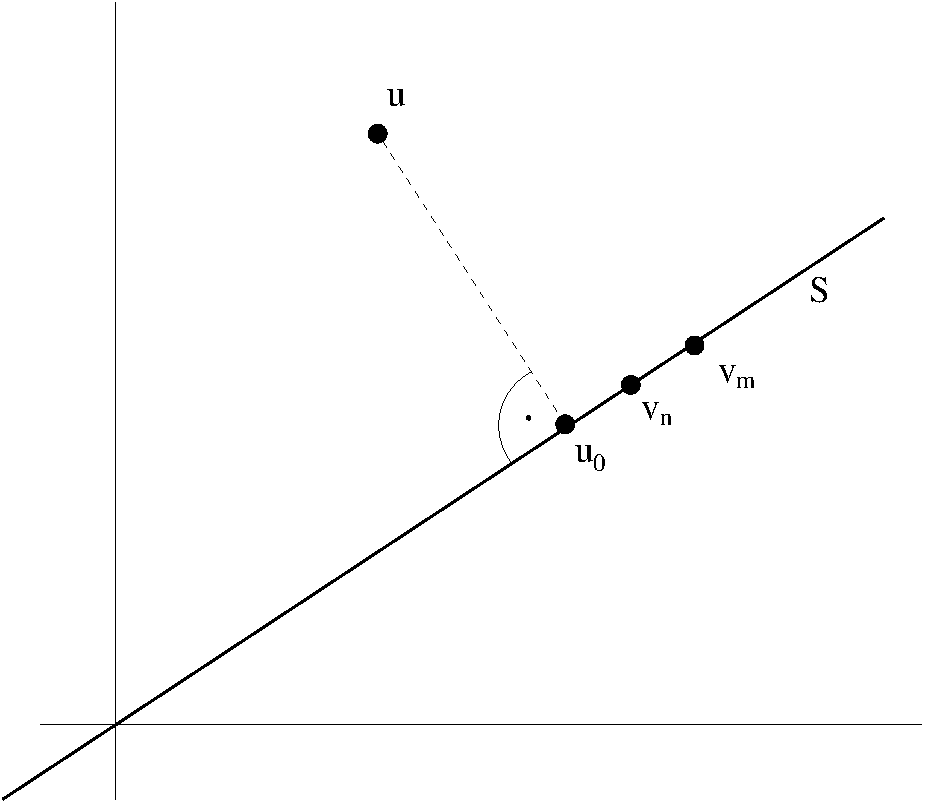
\includegraphics[height=4cm]{pictures/project}
\end{center}


We first check that there holds
$$
\| v_n - v_m \|^2 = 2 \, \| v_n - u \|^2 + 2 \, \| v_m - u \|^2 - 4 \,  \| \tfrac{1}{2}(v_n+v_m) - u \|^2.
$$
Since $\tfrac{1}{2} (v_n+v_m) \in S$, there holds $\| \tfrac{1}{2} (v_n+v_m) - u \| \geq d$.
We proof that $(v_n)$ is a Cauchy sequence:
Fix $\eps > 0$, choose $N \in \setN$ such that for $n > N$ there holds
$\| u - v_n \|^2 \leq d^2 + \eps^2$. Thus for all $n,m > N$ there holds
$$
\| v_n - v_m \|^2 \leq 2 (d^2+\eps^2) + 2 (d^2 + \eps^2) - 4 d^2 = 4 \eps^2.
$$ 
Thus, $v_n$ converge to some $u_0 \in V$. Since $S$ is closed, $u_0 \in S$.
By continuity of the norm, $\| u - u_0 \| = d$.

\medskip
Fix some $0 \neq w \in S$, and define $\varphi(t) := \| u - \underbrace{u_0 - t w}_{\in S} \|^2$.
$\varphi(\cdot)$ is a convex function, it takes its unique minimum $d$ at $t=0$. Thus
$$
0 = \frac{d \varphi(t)}{dt}|_{t=0} = \{ 2 (u-u_0, w) - 2 t (w,w) \} |_{t=0} = 
   2 (u-u_0,w)
$$ 
We obtained $u-u_0 \bot S$. If there were two minimizers $u_0 \neq u_1$, 
then $u_0-u_1 = (u_0-u) - (u_1-u) \bot S$ and $u_0-u_1 \in S$, which implies
$u_0-u_1 = 0$, a contradiction.
\hfill $\Box$

\bigskip
Theorem~\ref{theo_proj} says that given an $u \in V$, we can uniquely
decompose it as
$$
u = u_0 + u_1, \qquad u_0 \in S \quad u_1 \in S^\bot
$$
This allows to define the operators $P_S : V \rightarrow S$ and $P_S^\bot : V \rightarrow S^\bot$ as 
$$
P_S u := u_0 \qquad P_S^\bot u := (I - P_S) u = u_1
$$

\begin{theorem} $P_S$ and $P_S^\bot$ are linear operators. 
\end{theorem}

\begin{definition} A linear operator $P$ is called a {\bf projection} if $P^2 = P$.
A projector is called {\bf orthogonal}, if $(Pu,v) = (u,Pv)$.
\end{definition}
\begin{lemma} The operators $P_S$ and $P_S^\bot$ are both orthogonal 
projectors.
\end{lemma}
\noindent
{\em Proof:} For $u \in S$ there holds $P_S u = u$. Since $P_S u \in S$, there holds $P_S^2 u = P_S u$. It is orthogonal since
$$
(P_Su,v) = (P_Su,v-P_Sv+P_Sv) = (\underbrace{P_S u}_{\in S}, \underbrace{v-P_Sv}_{\in S^\bot}) + (P_Su,P_Sv) = (P_Su,P_Sv).
$$
With the same argument there holds $(u,P_Sv) = (P_Su,P_Sv)$.
The co-projector $P_S^\bot = I - P_S$ is a projector since
$$
(I-P_S)^2 = I - 2 P_S + P_S^2 = I - P_S.
$$
It is orthogonal since $((I-P_S) u,v) = (u,v)-(P_Su,v) =
        (u,v)-(u,P_Sv) = (u,(I-P_S)v)$
\hfill $\Box$

\section{Riesz Representation Theorem}
Let $u \in V$. Then, we can define the related continuous linear
functional~$l_u(\cdot) \in V^\ast$ by
$$
l_u (v) := (u,v)_V \qquad \forall \, v \in V.
$$
The opposite is also true:
\begin{theorem} {\bf Riesz Representation Theorem.} Any continuous linear
functional $l$ on a Hilbert space $V$ can be represented uniquely as
\begin{equation}
\label{equ_rieszrep}
l(v) = (u_l,v)
\end{equation}
for some $u_l \in V$. Furthermore, we have
$$
\| l \|_{V^\ast} = \| u_l \|_V.
$$
\end{theorem}
\noindent
{\em Proof:} First, we show uniqueness. Assume that $u_1 \neq u_2$ both
fulfill (\ref{equ_rieszrep}). This leads to the contradiction
\begin{eqnarray*}
0 & = & l(u_1-u_2) - l(u_1-u_2) \\
  & = & (u_1,u_1-u2) - (u_2,u_1-u_2) = \| u_1 - u_2 \|^2.
\end{eqnarray*}
Next, we construct the $u_l$. For this, define 
$S := \operatorname{ker} l$. This is a closed subspace. 

\noindent
Case 1: $S^\bot = \{ 0 \}$. Then, $S = V$, i.e., $l = 0$. So take $u_l = 0$.

\noindent
Case 2: $S^\bot \neq \{ 0 \}$. Pick some $0 \neq z \in S^\bot$. There
holds $l(z) \neq 0$ (otherwise, $z \in S \cap S^\bot = \{ 0 \}$).
Now define 
$$
u_l := \frac{l(z)}{\|z\|^2} z \qquad \in S^\bot
$$
Then
\begin{eqnarray*}
(u_l,v) & = & (\underbrace{u_l}_{S^\bot}, \underbrace{v - l(v)/l(z) z}_S) + (u_l,l(v)/l(z)z) \\
& = & l(z) / \| z\|^2 (z,l(v)/l(z) z) \\
& = & l(v)
\end{eqnarray*}
Finally, we prove $\|l\|_{V^\ast} = \| u_l \|_V$:
$$
\|l\|_{V^\ast} = \sup_{0 \neq v \in V} \frac{l(v)}{\|v\|}
        = \sup_v \frac{(u_l,v)_V}{\|v\|_V} \leq \| u_l \|_V
$$
and
$$
\| u_l \| = \frac{l(z)}{\|z\|^2}  \|z\| = \frac{l(z)}{\|z\|} \leq \| l \|_{V^\ast}.
$$
% \hfill $\Box$

\section{Symmetric variational problems}
Take the function space $C^1(\Omega)$, and define the bilinear form
$$
A(u,v) := \int_\Omega \nabla u \nabla v + \int_\Gamma u v \, ds
$$
and the linear form
$$
f(v) := \int_\Omega f v \, dx
$$
The bilinear form is non-negative, and $A(u,u) = 0$ implies $u = 0$.
Thus, $A(\cdot,\cdot)$ is an inner product, and provides the
norm $\|v\|_A := A(v,v)^{1/2}$. The normed vector space $(C^1, \|.\|_A)$
is not complete. Define
$$
V := \overline{C^1(\Omega)}^{\|.\|_A},
$$
which is a Hilbert space per definition. If we can show that there exists
a constant $c$ such that
$$
f(v) = \int_\Omega f v \, dx \leq c \| v \|_A \qquad \forall \, v \in V
$$
then $f(.)$ is a continuous linear functional on $V$.
We will prove this later. In this case, the Riesz representation theorem 
tells that there exists an unique $u \in V$ such that
$$
A(u,v) = f(v).
$$
This shows that the weak form has a unique solution in $V$.

Next, take the finite dimensional ($\Rightarrow$ closed) finite element subspace $V_h \subset V$.
The finite element solution $u_h \in V_h$ was defined by
$$
A(u_h,v_h) = f(v_h) \qquad \forall \, v_h \in V_h,
$$
This means
$$
A(u-u_h, v_h) = A(u,v_h) - A(u_h,v_h) = f(v_h) - f(v_h) = 0
$$
$u_h$ is the projection of $u$ onto $V_h$, i.e.,
$$
\| u - u_h \|_A \leq \| u - v_h \|_A \qquad \forall \, v_h \in V_h
$$
The error $u - u_h$ is orthogonal to $V_h$.

\section{Coercive variational problems}
%
In this chapter we discuss variational problems posed in Hilbert spaces.
Let $V$ be a Hilbert space, and let $A(\cdot,\cdot) : V \times V \rightarrow \setR$ be
a bilinear form which is
\begin{itemize}
\item coercive (also known as elliptic)
\begin{equation}
A(u,u) \geq \alpha_1 \| u \|_V^2 \qquad \forall \, u \in V,
\end{equation}
\item and continuous
\begin{equation}
A(u,v) \leq \alpha_2 \| u \|_V  \, \| v \|_V \qquad \forall \, u , v \in V,
\end{equation}
\end{itemize}
with bounds $\alpha_1$ and $\alpha_2$ in $\setR^+$. It is not necessarily symmetric.
Let $f(.) : V \rightarrow \setR$ be a continuous linear form on $V$, i.e., 
$$
f(v) \leq \| f \|_{V^\ast} \| v \|_V.
$$
We are posing the variational problem: find $u \in V$ such that
$$
A(u,v) = f(v) \qquad \forall \, v \in V.
$$

\begin{example} 
Diffusion-reaction equation: 
\end{example}
\noindent
Consider the PDE
$$
-\opdiv (a(x) \nabla u) + c(x) u = f \qquad \mbox{in } \Omega,
$$
with Neumann boundary conditions. Let $V$ be the Hilbert space generated 
by the inner product $(u,v)_V := (u,v)_{L_2}+ (\nabla u , \nabla v)_{L_2}$. 
The variational formulation of the PDE involves the bilinear form
$$
A(u,v) = \int_{\Omega} (a(x) \nabla u) \cdot \nabla v \, dx + \int_\Omega c(x) u v \, dx.
$$
Assume that the coefficients $a(x)$ and $c(x)$ fulfill 
$a(x) \in \setR^{d \times d}$, $a(x)$ symmetric and $\lambda_1 \leq \lambda_{\min} (a(x)) \leq \lambda_{\max} (a(x)) \leq \lambda_2$, and 
$c(x)$ such that $\gamma_1 \leq c(x) \leq \gamma_2$ almost everywhere. 
Then $A(\cdot,\cdot)$ is coercive with constant
$\alpha_1 = \min \{ \lambda_1, \gamma_1 \}$ and $\alpha_2 = \max \{ \lambda_2, \gamma_2 \}$.
\begin{example}  \label{example_diffconv}
Diffusion-convection-reaction equation:
\end{example}
\noindent
The partial differential equation
$$
-\Delta u + b \cdot \nabla u + u  = f \qquad \mbox{in} \; \Omega
$$
with Dirichlet boundary conditions $u = 0$ on $\partial \Omega$ leads to the
bilinear form
$$
A(u,v) = \int \nabla u \, \nabla v \, dx + \int b \cdot \nabla u \, v \, dx + \int u v \, dx.
$$
If $\opdiv b \leq 0$, what is an important case arising from incompressible flow
fields ($\opdiv \, b = 0$), then $A(\cdot,\cdot)$ is coercive and continuous w.r.t. the same norm as above.

\bigskip

Instead of the linear form $f(\cdot)$, we will often write $f \in V^\ast$. The evaluation is written as the duality product 
$$
\left< f , v \right>_{V^\ast \times V} = f(v).
$$

\begin{lemma}A continuous bilinear form $A(\cdot,\cdot) : V \times V \rightarrow \setR$
induces a continuous linear operator $A : V \rightarrow V^\ast$ via
$$
\left< A u, v \right> = A(u,v) \qquad \forall \, u,v \in V.
$$
The operator norm $\| A \|_{V \rightarrow V^\ast}$ is bounded by the continuity bound $\alpha_2$ of $A(\cdot,\cdot)$. 
\end{lemma}
\noindent
{\em Proof:} For every $u \in V$, $A(u,\cdot)$ is a bounded linear form on $V$
with norm
$$
\| A(u,\cdot) \|_{V^\ast} = 
\sup_{v \in V} \frac{A(u,v)}{ \| v \|_V} 
\leq \sup_{v \in V} \frac{\alpha_2 \| u \|_V \, \| v \|_V }{ \| v \|_V} 
= \alpha_2 \| u \|_V
$$
Thus, we can define the operator $A : u \in V \rightarrow A(u,\cdot) \in V^\ast$. 
It is linear, and its operator norm is bounded by
\begin{eqnarray*}
\| A \|_{V \rightarrow V^\ast} & = &
\sup_{u\in V} \frac{ \| A u \|_{V^\ast}}{\| u \|_V} =
\sup_{u\in V} \sup_{v \in V} \frac{ \left< A u, v\right>_{V^\ast \times V} } {\| u \|_V \, \| v \|_V} \\
& = & \sup_{u\in V} \sup_{v \in V} \frac{ A (u,v) } {\| u \|_V \, \| v \|_V} \leq
\sup_{u\in V} \sup_{v\in V} \frac{ \alpha_2 \| u \|_V \| v \|_V } {\| u \|_V \, \| v \|_V} = \alpha_2.
\end{eqnarray*}
\hfill $\Box$

Using this notation, we can write the variational problem as operator equation: find $u \in V$ such that
$$
A u = f \qquad (\mbox{in } V^\ast).
$$

\begin{theorem}[Banach's contraction mapping theorem] Given a Banach space
$V$ and a mapping $T : V \rightarrow V$, satisfying the Lipschitz condition
$$
\| T(v_1) - T(v_2) \| \leq L \, \| v_1 - v_2 \| \qquad \forall  \, v_1, v_2 \in V
$$
for a fixed $L \in [0,1)$. Then there exists a unique $u \in V$ such that
$$
u = T(u),
$$
i.e. the mapping $T$ has a unique fixed point $u$. The iteration $u^1 \in V$ given, compute
$$
u^{k+1} := T(u^k)
$$
converges to $u$ with convergence rate $L$:
$$
\| u - u^{k+1} \| \leq L \| u - u^k \|
$$
\end{theorem}


\begin{theorem}[Lax Milgram] Given a Hilbert space $V$, a coercive and continuous bilinear form $A(\cdot,\cdot)$, and a continuous linear form $f(.)$. Then there exists a unique $u \in V$ solving
$$
A(u,v) = f(v) \qquad \forall \, v \in V.
$$
There holds 
\begin{equation} \label{equ_lax_milgram_bound}
\| u \|_V \leq \alpha_1^{-1} \| f \|_{V^\ast}
\end{equation}
\end{theorem}
{\em Proof:} Start from the operator equation $A u = f$. Let $J_V : V^\ast \rightarrow V$ be the Riesz isomorphism defined by
$$
(J_V g, v)_V = g(v) \qquad \forall \, v \in V, \;  \forall \, g \in V^\ast.
$$
Then the operator equation is equivalent to
$$
J_V A u = J_V f \qquad (\mbox{in } V),
$$
and to the fixed point equation (with some $0 \neq \tau \in \setR$ chosen below)
\begin{equation} \label{equ_fixedpointequ}
u = u - \tau J_V (A u - f).
\end{equation}
We will verify that
$$
T (v) := v - \tau J_V (A v - f)
$$
is a contraction mapping, i.e., $\| T (v_1) - T (v_2) \|_V \leq L \| v_1 - v_2 \|_V$ 
with some Lipschitz constant $L \in [0,1)$.
Let $v_1, v_2 \in V$, and set $v = v_1 - v_2$. Then
\begin{eqnarray*}
\| T (v_1) - T (v_2) \|_V^2 
& = & \| \{ v_1 - \tau J_V (A v_1 - f) \} - \{ v_2 - \tau J_V (A v_2 -f) \} \|_V^2 \\
& = & \| v - \tau J_V A v \|_V^2 \\
& = & \| v \|_V^2 - 2 \tau (J_V A v, v)_V + \tau^2 \| J_V A v \|_V^2 \\
& = & \| v \|_V^2 - 2 \tau \left< A v , v \right> + \tau^2 \| A v \|_{V^\ast}^2 \\
& = & \| v \|_V^2 - 2 \tau A(v,v) + \tau^2 \| A v \|_{V^\ast}^2 \\
& \leq & \| v \|_V^2 - 2 \tau \alpha_1 \| v \|_V^2 + \tau^2 \alpha_2^2 \| v \|_V^2 \\
& = & (1 - 2 \tau \alpha_1 + \tau^2 \alpha_2^2) \| v_1 - v_2 \|_V^2
\end{eqnarray*}
Now, we choose $\tau = \alpha_1 / \alpha_2^2$, and obtain a Lipschitz constant
$$
L^2 = 1 - \alpha_1^2 / \alpha_2^2 \in [0,1).
$$
Banach's contraction mapping theorem state that (\ref{equ_fixedpointequ}) 
has a unique fixed point. Finally, we obtain the bound (\ref{equ_lax_milgram_bound}) from
$$
\| u \|_V^2 \leq \alpha_1^{-1} A(u,u) = \alpha_1^{-1} \, f(u) \leq \alpha_1^{-1} \| f\|_{V^\ast} \| u \|_V,
$$
and dividing by one factor $\|u\|$.
\hfill $\Box$

\subsection{Approximation of coercive variational problems}
Now, let $V_h$ be a closed subspace of $V$. We compute the
approximation $u_h \in V_h$ by the Galerkin method
\begin{equation}
A(u_h, v_h) = f(v_h) \qquad \forall \, v_h \in V_h.
\end{equation}
This variational problem is uniquely solvable by Lax-Milgram, 
since, $(V_h,\|.\|_V)$ is 
a Hilbert space, and continuity and coercivity on $V_h$ are inherited
from the original problem on $V$.


The next theorem says, that the solution defined by the Galerkin method is,
up to a constant factor, as good as the best possible approximation in the
finite dimensional space.

\begin{theorem}[Cea] The approximation error of the Galerkin method
is quasi optimal
$$
\| u - u_h \|_V \leq \alpha_2 / \alpha_1 \inf_{v \in V_h} \| u - v_h \|_V
$$
\end{theorem}
{\em Proof:} A fundamental property is the Galerkin orthogonality
$$
A(u-u_h, w_h) = A(u,w_h) - A(u_h, w_h) = f(w_h) - f(w_h) = 0
\qquad \forall \, w_h \in V_h.
$$
Now, pick an arbitrary $v_h \in V_h$, and bound
\begin{eqnarray*}
\| u - u_h \|_V^2 & \leq & \alpha_1^{-1} A(u-u_h, u-u_h) \\
& = & \alpha_1^{-1} A(u-u_h, u-v_h) + \alpha_1^{-1} A(u-u_h, \underbrace{v_h-u_h}_{\in V_h}) \\
& \leq &  \alpha_2 / \alpha_1 \, \| u - u_h \|_V \| u - v_h \|_V.
\end{eqnarray*}
Divide one factor $\|u - u_h\|$. Since $v_h \in V_h$ was arbitrary, the estimation
holds true also for the infimum in $V_h$.
\hfill $\Box$

\bigskip
If $A(\cdot,\cdot)$ is additionally symmetric, then it is an inner product. In this
case, the coercivity and continuity properties are equivalent to
$$
\alpha_1 \| u \|_V^2 \leq A(u,u) \leq \alpha_2 \, \| u \|_V^2
\qquad \forall \, u \in V.
$$
The generated norm $\|.\|_A$ is an equivalent norm to $\|.\|_V$. In the 
symmetric case, we can use the orthogonal projection with respect to 
$(.,.)_A$ to improve the bounds to
$$
\| u - u_h \|_V^2 \leq \alpha_1^{-1} \| u - u_h \|_A^2 \leq
        \alpha_1^{-1} \inf_{v_h \in V_h} \| u - v_h \|_A^2 \leq
        \alpha_2 / \alpha_1 \| u - v_h \|_V^2.
$$
The factor in the quasi-optimality estimate is now the square root of the
general, non-symmetric case.

\section{Inf-sup stable variational problems}

The coercivity condition is by no means a necessary condition for a
stable solvable system. A simple, stable problem with non-coercive
bilinear form is to choose $V = \setR^2$, and the bilinear form 
$B(u,v) = u_1 v_1 - u_2 v_2$. The solution of $B(u,v) = f^T v$ is 
$u_1 = f_1$ and $u_2 = -f_2$. We will follow the convention to call
coercive bilinear forms $A(\cdot,\cdot)$, and the more general ones $B(\cdot,\cdot)$.

Let $V$ and $W$ be Hilbert spaces, and $B(\cdot,\cdot) : V \times W \rightarrow \setR$ be a continuous bilinear form with bound
\begin{equation}
B(u,v) \leq \beta_2 \| u \|_V \| v \|_W \qquad \forall \, u \in V, \; \forall \, v \in W.
\end{equation}
The general condition is the {\bf inf-sup condition}
\begin{equation} \label{equ_infsup}
\inf_{u \in V \atop u \neq 0} \sup_{v \in W \atop v \neq 0}
\frac{ B(u,v) } { \| u \|_V \, \| v \|_W } \geq \beta_1.
\end{equation}

Define the linear operator $B : V \rightarrow W^\ast$ by $\left< B u, v \right>_{W^\ast \times W} = B(u,v)$. The inf-sup condition can be reformulated as
$$
\sup_{v \in W} \frac{ \left< B u, v \right> } { \| v \|_W } \geq \beta_1 \| u \|_V, \qquad \forall \, u \in V
$$
and, using the definition of the dual norm,
\begin{equation} \label{equ_stabb}
\| B u \|_{W^\ast} \geq \beta_1 \| u \|_V.
\end{equation}
We immediately obtain that $B$ is one to one, since
$$
B u = 0 \Rightarrow u = 0
$$
\begin{lemma} Assume that the continuous bilinear form $B(\cdot,\cdot)$ fulfills the
inf-sup condition (\ref{equ_infsup}). Then the according operator $B$ has
closed range.
\end{lemma}
{\em Proof:} Let $B u^n$ be a Cauchy sequence in $W^\ast$. From (\ref{equ_stabb}) we conclude that also $u^n$ is Cauchy in $V$. Since $V$ is complete, $u_n$
converges to some $u \in V$. By continuity of $B$, the sequence $B u^n$ converges to $B u \in W^\ast$.
\hfill $\Box$

The inf-sup condition (\ref{equ_infsup}) does not imply that $B$ is onto $W^\ast$. To insure that, we can pose an inf-sup condition the other way around:
\begin{equation} \label{equ_infsupb}
\inf_{v \in W \atop v \neq 0} \sup_{u \in V \atop u \neq 0}
\frac{ B(u,v) } { \| u \|_V \, \| v \|_W } \geq \beta_1.
\end{equation}
It will be sufficient to state the weaker condition
\begin{equation} \label{equ_infsup2}
\sup_{u \in V \atop u \neq 0}
\frac{ B(u,v) } { \| u \|_V \, \| v \|_W } > 0 \qquad \forall \, v \in W.
\end{equation}

\begin{theorem} \label{theo_infsup} 
Assume that the continuous bilinear form $B(\cdot,\cdot)$ fulfills
the inf-sup condition (\ref{equ_infsup}) and condition (\ref{equ_infsup2}). 
Then, the variational problem: find $u \in V$ such that
\begin{equation} \label{equ_bigsystem}
B(u,v) = f(v) \qquad \forall \, v \in W
\end{equation}
has a unique solution. The solution depends continuously on the right hand
side:
$$
\| u \|_V \leq \beta_1^{-1} \| f \|_{W^\ast}
$$
\end{theorem}
{\em Proof:} We have to show that the range $R(B) = W^\ast$. The Hilbert
space $W^\ast$ can be split into the orthogonal, closed subspaces
$$
W^\ast = R(B) \oplus R(B)^\bot.
$$
Assume that there exists some $0 \neq g \in R(B)^\bot$. This means that
$$
(B u, g)_{W^\ast} = 0 \qquad \forall \, u \in V.
$$
Let $v_g \in W$ be the Riesz representation of $g$, i.e., $(v_g, w)_W = g(w)$ for all $w \in W$. This $v_g$ is in contradiction to the assumption 
(\ref{equ_infsup2})
$$
\sup_{u \in V} \frac{B(u,v_g)}{ \| u \|_V} = 
\sup_{u \in V} \frac{(Bu,g)_{W^\ast}}{ \| u \|_V} = 
0.
$$
Thus, $R(B)^\bot = \{ 0 \}$ and $R(B) = W^\ast$.
\hfill $\Box$

\begin{example}A coercive bilinear form is inf-sup stable.
\end{example}
\begin{example}A complex symmetric variational problem:
\end{example}
\noindent
Consider the complex valued PDE 
$$
-\Delta u + i u = f,
$$
with Dirichlet boundary conditions, $f \in L_2$, and $i = \sqrt{-1}$. The
weak form for the real system $u = (u_{r}, u_i) \in V^2$ is
\begin{equation}
\begin{array}{rcll}
(\nabla u_{r}, \nabla v_{r})_{L_2} + (u_i, v_{r})_{L_2} & = &
        (f,v_{r}) \qquad & \forall \, v_r \in V \\
(u_{r}, v_i)_{L_2} -(\nabla u_i, \nabla v_i)_{L_2} & = &
        -(f,v_i) & \forall \, v_i \in V
\end{array}
\end{equation}
We can add up both lines, and define the large bilinear form $B(\cdot,\cdot) : V^2 \times V^2 \rightarrow \setR$ by
$$
B ((u_r,u_i), (v_r, v_i)) = 
(\nabla u_{r}, \nabla v_{r}) + (u_i, v_{r}) + (u_{r}, v_i) -(\nabla u_i, \nabla v_i)
$$
With respect to the norm $\|v\|_V = ( \| v \|_{L_2}^2 + \| \nabla v \|_{L_2}^2)^{1/2}$, the bilinear form is continuous, and fulfills the inf-sup conditions
(exercises !)
Thus, the variational formulation: find $u \in V^2$ such that
$$
B(u,v) = (f,v_r) - (f,v_i) \qquad \forall \, v \in V^2
$$
is stable solvable.

\bigskip

\subsection{Approximation of inf-sup stable variational problems}
Again, to approximate (\ref{equ_bigsystem}), we pick finite dimensional
subspaces $V_h \subset V$ and $W_h \subset W$, and pose the finite dimensional
variational problem: find $u_h \in V_h$ such that
$$
B(u_h, v_h) = f(v_h) \qquad \forall \, v_h \in W_h.
$$
But now, in contrast to the coercive case, the solvability of the 
finite dimensional equation does not follow from the solvability conditions
of the original problem on $V \times W$. E.g., take the example in $\setR^2$
above, and choose the subspaces $V_h = W_h = \mbox{span} \{ (1,1) \}$. 

We have to pose an extra inf-sup condition for the discrete problem:
\begin{equation} \label{equ_infsuph}
\inf_{u_h \in V_h \atop u_h \neq 0} \sup_{v_h \in W_h \atop v_h \neq 0}
\frac{ B(u_h,v_h) } { \| u_h \|_V \, \| v_h \|_W } \geq \beta_{1h}.
\end{equation}
On a finite dimensional space, one to one is equivalent to onto, and we
can skip the second condition.

\begin{theorem} \label{theo_approxinfsup}
Assume that $B(\cdot,\cdot)$ is continuous with bound $\beta_2$, and 
$B(\cdot,\cdot)$ fulfills the discrete inf-sup condition with bound $\beta_{1h}$. 
Then there holds the quasi-optimal error estimate
\begin{equation}
\| u - u_h \| \leq (1 + \beta_2 / \beta_{1h}) \inf_{v_h \in V_h} \| u - v_h \|
\end{equation}
\end{theorem}
\noindent
{\em Proof:} Again, there holds the Galerkin orthogonality $B(u,w_h) = B(u_h,w_h)$ for all $w_h \in V_h$. Again, choose an arbitrary $v_h \in V_h$:
\begin{eqnarray*}
\| u - u_h \|_V & \leq & \| u - v_h \|_V + \| v_h - u_h \|_V \\
        & \leq & \| u - v_h \|_V + \beta_{1h}^{-1} 
                \sup_{w_h \in W_h} \frac{ B(v_h-u_h, w_h) } { \| w_h \|_V } \\
        & = &  \| u - v_h \|_V + \beta_{1h}^{-1} 
                \sup_{w_h \in W_h} \frac{ B(v_h-u, w_h) } { \| w_h \|_V } \\
        & \leq & \| u - v_h \|_V + \beta_{1h}^{-1}
                \sup_{w_h \in W_h} \frac{ \beta_2 \| v_h-u \|_V \, \| w_h \|_W } { \| w_h \|_W } \\
        & = & (1 + \beta_2 / \beta_{1h}) \| u - v_h\|_V.
\end{eqnarray*}

\chapter{Sobolev Spaces}
\label{sec_sobolev}
%
In this section, we introduce the concept of generalized derivatives, we
define families of normed function spaces, and prove inequalities between
them.
Let $\Omega$ be an open subset of $\setR^d$, either bounded or unbounded.

\section{Generalized derivatives}

Let $\alpha = (\alpha_1, \ldots , \alpha_d) \in \setN_0^d$ be a multi-index,
$| \alpha | = \sum \alpha_i$, 
and define the classical differential operator for functions in $C^\infty (\Omega)$
$$
D^\alpha = 
        \left( \frac{\partial}{\partial x_1} \right)^{\alpha_1} \cdots
        \left( \frac{\partial}{\partial x_n} \right)^{\alpha_d}.
$$
%
For a function $u \in C^(\Omega)$, the support is defined as 
$$
\operatorname{supp} \{ u \} := \overline{ \{ x \in \Omega : u(x) \neq 0 \} }.
$$
This is a compact set if and only if it is bounded. We say $u$ has
compact support in $\Omega$, if $\operatorname{supp} u \subset \Omega$.
If $\Omega$ is a bounded domain, then $u$ has compact support in $\Omega$
if and only if $u$ vanishes in a neighbourhood of $\partial \Omega$.

\medskip
\noindent
The space of smooth functions with compact support is denoted as
\begin{equation}
{\cal D} (\Omega) := C_0^\infty (\Omega) := 
\{ u \in C^\infty(\Omega) : \mbox{ $u$ has compact support in $\Omega$} \}.
\end{equation}
%
For a smooth function $u \in C^{|\alpha|}(\Omega)$, there holds the
formula of integration by parts
\begin{equation} \label{equ_intbyparts}
\int_\Omega D^\alpha u \varphi \, dx = (-1)^{|\alpha|} \int_\Omega u D^\alpha \varphi \, dx 
\qquad \forall \, \varphi \in {\cal D}(\Omega).
\end{equation}
The $L_2$ inner product with a function $u$ in $C(\Omega)$ defines the linear
functional on ${\cal D}$
$$
u(\varphi) := \left< u, \varphi \right>_{{\cal D}^\prime \times {\cal D}} := \int_\Omega u \varphi \, dx.
$$
We call these functionals in ${\cal D}^\prime$ distributions.
When $u$ is a function, we identify it with the generated distribution.
The formula (\ref{equ_intbyparts}) is valid for functions $u \in C^\alpha$.
The strong regularity is needed only on the left hand side. Thus, we use
the less demanding right hand side to extend the definition of differentiation
for distributions:

\begin{definition} For $u \in {\cal D}^\prime$, we define 
$g \in {\cal D}^\prime$ to be the generalized 
derivative $D_g^\alpha u$ of $u$ by
$$
\left<g, \varphi \right>_{{\cal D}^\prime \times {\cal D}} = 
(-1)^{|\alpha|} \left<u, D^\alpha \varphi \right>_{{\cal D}^\prime \times {\cal D}}  \qquad \forall \, \varphi \in {\cal D}
$$
\end{definition}
%
\noindent
If $u \in C^\alpha$, then $D_g^\alpha$ coincides with $D^\alpha$. 

\noindent
The function space of {\bf locally integrable} functions on $\Omega$ 
is called
$$
L_1^{loc} (\Omega) = \{ u : u_K \in L_1(K) \; \forall \mbox{ compact } K 
\subset \Omega \}.
$$
It contains functions which can behave very badly near $\partial \Omega$.
E.g., $e^{e^{1/x}}$ is in $L_{loc}^1 (0,1)$. If $\Omega$ is unbounded, then
the constant function $1$ is in $L_1^{loc}$, but not in $L_1$.


\begin{definition} For $u \in L_1^{loc}$, we call $g$ the weak derivative
$D_w^\alpha u$, if $g \in L_1^{loc}$ satisfies
$$
\int_\Omega g(x) \varphi(x) \, dx =
(-1)^{|\alpha|} \int_\Omega u(x) D^\alpha \varphi (x) \, dx  \qquad \forall \, \varphi \in {\cal D}.
$$
\end{definition}
The weak derivative is more general than the classical derivative, but more
restrictive than the generalized derivative.


\begin{example} 
Let $\Omega = (-1,1)$ and 
$$
u(x) = \left\{ 
        \begin{array}{cl}
        1+x & \quad x \leq 0 \\
        1-x & \quad x > 0
        \end{array}
        \right\}
$$
Then, 
$$
g(x) = \left\{ 
        \begin{array}{cl}
        1 & \quad x \leq 0 \\
        -1 & \quad x > 0
        \end{array}
        \right\}
$$
is the first generalized derivative $D^1_g$ of $u$, which is also
a weak derivative. The second generalized derivative $h$ is 
$$
\left< h, \varphi \right> = -2 \varphi(0)  \qquad \forall \, \varphi \in {\cal D}
$$
It is not a weak derivative.
\end{example}

In the following, we will focus on weak derivatives. Unless it is essential
we will skip the sub-scripts $w$ and $g$.


\section{Sobolev spaces}

For $k \in \setN_0$ and $1 \leq p < \infty$, we define the Sobolev norms 
$$
\| u \|_{W_p^k(\Omega)} := \left( \sum_{|\alpha| \leq k} \| D^\alpha u \|_{L_p}^p \right)^{1/p},
$$
for $k \in \setN_0$ we set
$$
\| u \|_{W_\infty^k(\Omega)} := \max_{|\alpha| \leq k}  \| D^\alpha u \|_{L_\infty}.
$$
In both cases, we define the {\bf Sobolev spaces} via
$$
W_p^k(\Omega) = \{ u \in L_1^{loc} : \| u \|_{W_p^k} < \infty \}
$$

In the previous chapter we have seen the importance of complete spaces.
This is the case for Sobolev spaces:
\begin{theorem} The Sobolev space $W_p^k(\Omega)$ is a Banach space.
\end{theorem}
\noindent
{\em Proof:} Let $v_j$ be a Cauchy sequence with respect to $\| \cdot \|_{W_p^k}$. This implies that $D^\alpha v_j$ is a Cauchy sequence in $L_p$, and 
thus converges to some $v^\alpha$ in $\|. \|_{L_p}$. 

We verify that $D^\alpha v_j \rightarrow v^\alpha$ implies 
$\int_\Omega D^\alpha v_j \varphi \, dx \rightarrow \int_\Omega v^\alpha \varphi \, dx$ for all $\varphi \in {\cal D}$. Let $K$ be the compact support 
of $\varphi$. There holds 
\begin{eqnarray*}
\int_\Omega (D^\alpha v_j - v^\alpha) \varphi \, dx & = & 
\int_{K} (D^\alpha v_j - v^\alpha) \varphi \, dx  \\
& \leq & \| D^\alpha v_j - v^\alpha \|_{L_1(K)} \| \varphi \|_{L_\infty} \\
& \leq & \| D^\alpha v_j - v^\alpha \|_{L_p(K)} \| \varphi \|_{L_\infty}
\rightarrow 0
\end{eqnarray*}
Finally, we have to check that $v^\alpha$ is the weak derivative of $v$:
\begin{eqnarray*}
\int v^\alpha \varphi \, dx & = & 
        \lim_{j\rightarrow \infty} \int_\Omega D^\alpha v_j \varphi \, dx \\
        & = & \lim_{j\rightarrow \infty} (-1)^{|\alpha|} \int_\Omega v_j D^\alpha \varphi \, dx = \\
        & = & (-1)^\alpha \int_\Omega v  D^\alpha \varphi \, dx.
\end{eqnarray*}
\hfill $\Box$

\bigskip

An alternative definition of Sobolev spaces were to take the closure
of smooth functions in the domain, i.e.,
$$
\widetilde W_p^k := \overline{ \{ C^\infty (\Omega) : \|.\|_{W_p^k} \leq \infty \} }^{\|.\|_{W_p^k}}.
$$
A third one is to take continuously differentiable functions up to the boundary
$$
\widehat W_p^k := \overline{ C^\infty (\overline{\Omega}) }^{\|.\|_{W_p^k}}.
$$

Under moderate restrictions, these definitions lead to the same spaces:
\begin{theorem} Let $1 \leq p < \infty$. Then $\widetilde W_p^k  = W_p^k$.
\end{theorem}

\begin{definition} The domain $\Omega$ has a {\bf Lipschitz boundary}, $\partial \Omega$, if there exists a collection of open sets $O_i$, a positive parameter $\eps$, an integer $N$ and a finite number $L$, such that for all $x \in \partial \Omega$ the ball of radius $\eps$ centered at $x$ is contained in some $O_i$, no more than $N$ of the sets $O_i$ intersect non-trivially, and each 
part of the boundary $O_i \cap \Omega$ is a graph of a Lipschitz function $\varphi_i : \setR^{d-1} \rightarrow \setR$ with Lipschitz norm bounded by $L$.
\end{definition}

\begin{theorem} Assume that $\Omega$ has a Lipschitz boundary, and let $1 \leq p < \infty$. Then  $\widehat W_p^k  = W_p^k$.
\end{theorem}


The case $W_2^k$ is special, it is a Hilbert space. We denote it by
$$
H^k(\Omega) := W_2^k(\Omega).
$$
The inner product is 
$$
(u,v)_{H^k} := \sum_{|\alpha| \leq k} (D^\alpha u, D^\alpha v)_{L_2}
$$
In the following, we will prove most theorems for the Hilbert spaces $H^k$,
and state the general results for $W_p^k$.

\section{Trace theorems and their applications}
We consider boundary values of functions in Sobolev spaces. Clearly,
this is not well defined for $H^0 = L_2$. But, as we will see, in
$H^1$ and higher order Sobolev spaces, it makes sense to talk about $u
|_{\partial \Omega}$. The definition of traces is essential to
formulate boundary conditions of PDEs in weak form.


We start in one dimension. Let $u \in C^1 ([0,h])$ with some $h > 0$. Then,
we can bound 
\begin{eqnarray*}
u(0) & = & \left(1 - \frac{x}{h} \right) u(x) |_{x=0} = 
        - \int_0^h \left\{ \left(1-\frac{x}{h} \right) u(x) \right\}^\prime \, dx \\
        & = & \int_0^h  \frac{-1}{h} u(x) + \left(1-\frac{x}{h} \right) u^\prime(x)  \, dx \\
        & \leq & \left\| \frac{1}{h} \right\|_{L_2} \| u \|_{L_2} + 
                \left\| 1-\frac{x}{h} \right\|_{L_2} \| u^\prime \|_{L_2} \\
        & \eqc & h^{-1/2} \| u \|_{L_2(0,h)} + h^{1/2} \| u^\prime \|_{L_2(0,h)}.
\end{eqnarray*}
This estimate includes the scaling with the interval length $h$. 
If we are not interested in the scaling, we apply Cauchy-Schwarz in $\setR^2$,
and combine the $L_2$ norm and the $H^1$ semi-norm $\|u^\prime\|_{L_2}$ to the full $H^1$ norm and obtain
$$
|u(0)| \leq \sqrt{h^{-1/2} + h^{1/2} } \sqrt{ \| u \|_{L_2}^2 + \| u^\prime \|_{L_2}^2 } = c \, \| u \|_{H^1}.
$$
Next, we extend the trace operator to the whole Sobolev space $H^1$:
\begin{theorem} There is a well defined and continuous trace operator
$$
\optr : H^1((0,h)) \rightarrow \setR
$$
whose restriction to $C^1([0,h])$ coincides with
$$
u \rightarrow u(0).
$$
\end{theorem}
{\em Proof:} Use that $C^1([0,h])$ is dense in $H^1(0,h)$. Take a sequence
$u_j$ in $C^1([0,h])$ converging to $u$ in $H^1$-norm. The values 
$u_j(0)$ are Cauchy, and thus converge to an $u_0$. The limit is independent 
of the choice of the sequence $u_j$. This allows to define $\optr u := u_0$.
\hfill $\Box$

\medskip

Now, we extend this 1D result to domains in more dimensions. Let
$\Omega$ be bounded, $\partial \Omega$ be Lipschitz, and consists of
$M$ pieces $\Gamma_i$ of smoothness $C^1$. 

We can construct the following covering of a neighbourhood of 
$\partial \Omega$ in $\Omega$: Let $Q = (0,1)^2$. For $1 \leq i \leq M$, 
let $s_i \in C^1 (Q, \Omega)$ be invertible and such that $\left\| s_i^\prime \right\|_{L_\infty} \leq c$,
 $\| (s_i^\prime)^{-1} \|_{L_\infty} \leq c$, and $\operatorname{det} s_i^\prime > 0$. The domains $S_i := s_i(Q)$ are
such that $s_i( (0,1) \times \{ 0 \} ) = \Gamma_i$, and the parameterizations
match on $s_i( \{ 0,1 \} \times (0,1) )$.

\begin{theorem}
There exists a well defined and continuous operator
$$
\optr : H^1 (\Omega) \rightarrow L_2(\partial \Omega)
$$
which coincides with $u|_{\partial \Omega}$ for $u \in C^1(\overline{\Omega})$.
\end{theorem}
\noindent
{\em Proof:} Again, we prove that 
$$
\optr : C^1(\overline{\Omega}) \rightarrow L_2(\partial \Omega)
        : u \rightarrow u |_{\partial \Omega}
$$
is a bounded operator w.r.t. the norms $\|.\|_{H^1}$ and $L_2$, and conclude by
density.
We use the partitioning of $\partial \Omega$ into the pieces $\Gamma_i$, and
transform to the simple square domain $Q = (0,1)^2$. 
Define the functions $u_i$ on $Q = (0,1)^2$ as
$$
\tilde u_i (\tilde x) = u(s_i(\tilde x))
$$
We transfer the $L_2$ norm to the simple domain:
\begin{eqnarray*}
\| \optr u \|_{L_2(\partial \Omega)}^2 & = & 
%       \sum_{i=1}^M \| u \|_{L_2(\Gamma_i)}^2 =
        \sum_{i=1}^M \int_{\Gamma_i} u(x)^2 \, dx \\
        & = & 
        \sum_{i=1}^M \int_0^1 u(s_i(\xi,0))^2 \left| \frac{\partial s_i}{\partial \xi} (\xi, 0) \right| \, d \xi \\
        & \leq & c \sum_{i=1}^M \int_0^1 \tilde u_i(\xi,0)^2  \, d \xi  
\end{eqnarray*}
To transform the $H^1$-norm, 
we differentiate with respect to $\tilde x$ by applying the chain rule
$$
\frac{d \tilde u_i}{d \tilde x} (\tilde x) = \frac{d u}{d x} (s_i(\tilde x))
 \frac{d s_i}{d \tilde x} (\tilde x).
$$
Solving for $\frac{d u }{d x}$ is
$$
\frac{d u }{dx} (s_i(\tilde x)) = \frac{ d \tilde u_i}{d \tilde x}(\tilde x)
\left( \frac{ds }{d \tilde x} \right)^{-1} (\tilde x)
% \nabla_x u(s_i(\xi,\eta)) = \nabla_{(\xi,\eta)} \tilde u_i (\xi,\eta)\, (\nabla s)^{-1}.
$$
The bounds onto $s^\prime$ and $(s^\prime)^{-1}$ imply that
$$
c^{-1} \, |\nabla_x u | \leq | \nabla_{\tilde x} \tilde u | \leq c \, | \nabla_x u |
$$
We start from the right hand side of the stated estimate:
\begin{eqnarray*}
\| u \|_{H^1(\Omega)}^2 & \geq &
 \sum_{i=1}^M \int_{S_i} | \nabla_x u |^2 \, dx \\
 & = & \sum_{i=1}^M \int_Q \left| \nabla_x u (s_i (\tilde x)) \right|^2    \det ( s^\prime ) \, d \tilde x \\
 & \geq & c \,  \sum_{i=1}^M \int_Q \left| \nabla_{\tilde x} \tilde u (\tilde x) \right| ^2  \, d \tilde x
\end{eqnarray*}
We got a lower bound for $\det (s^\prime) = (\det (s^\prime)^{-1})^{-1}$ from the upper bound for $(s^\prime)^{-1}$.

It remains to prove the trace estimate on $Q$. Here, we apply the previous
one dimensional result 
$$
| u(\xi, 0)|^2 \leq c \int_0^1 \left\{ u(\xi,\eta)^2 + \left(\frac{\partial u(\xi,\eta)}{\partial \eta}\right)^2 \right\} \, d \eta
\qquad \forall \, \xi \in (0,1)
$$
The result follows from integrating over $\xi$
\begin{eqnarray*}
\int_0^1 |  u(\xi, 0)|^2 \, d\xi & \leq & 
 c \, \int_0^1  \int_0^1  \left\{ u(\xi,\eta)^2 + \left(\frac{\partial u(\xi,\eta)}{\partial \eta}\right)^2 \right\} \, d \eta \, d \xi \\
        & \leq & c \, \| u \|_{H^1(Q)}^2.
\end{eqnarray*}
\hfill $\Box$


\bigskip

Considering the trace operator from $H^1(\Omega)$ to $L_2(\partial \Omega)$ is
not sharp with respect to the norms. We will improve the embedding later.

\bigskip

By means of the trace operator we can define the sub-space
$$
H_0^1(\Omega) = \{ u \in H^1(\Omega) : \optr \, u = 0 \}
$$
It is a true sub-space, since $u = 1$ does belong to $H^1$, but not to $H_0^1$.
It is a closed sub-space, since it is the kernel of a continuous operator.


\bigskip

By means of the trace inequality, one verifies that the linear functional
$$
g(v) := \int_{\Gamma_N} g \, \optr \, v \, dx
$$
is bounded on $H^1$. 


\subsubsection{Integration by parts}
The definition of the trace allows us to perform integration by
parts in $H^1$:
$$
\int_{\Omega} \nabla u \varphi \, dx = -\int_\Omega u \opdiv \, \varphi \, dx 
        + \int_{\partial \Omega} \optr u \, \varphi \cdot n \, dx 
\qquad \forall \, \varphi \in [C^1(\overline{\Omega})]^2
$$
The definition of the weak derivative (e.g. the weak gradient) looks similar.
It allows only test functions $\varphi$ with compact support in $\Omega$, i.e.,
having zero boundary values. Only by choosing a normed space, for which the 
trace operator is well defined, we can state and prove integration by parts.
Again, the short proof is based on the density of $C^1(\overline \Omega)$ 
in $H^1$.

\subsubsection{Sobolev spaces over sub-domains}
Let $\Omega$ consist of $M$ Lipschitz-continuous sub-domains $\Omega_i$ 
such that
\begin{itemize}
\item $\overline \Omega = \cup_{i=1}^M \overline \Omega_i$
\item $\Omega_i \cap \Omega_j = \emptyset \quad \mbox{ if } i \neq j$
\end{itemize}
The interfaces are $\gamma_{ij} = \overline \Omega_i \cap \overline \Omega_j$.
The outer normal vector of $\Omega_i$ is $n_i$.

\begin{theorem} \label{theo_subdomainh1}
Let $u \in L_2(\Omega)$ such that
\begin{itemize}
\item
$u_i := u|_{\Omega_i}$ is in $H^1(\Omega_i)$, and $g_i = \nabla u_i$ is its
weak gradient
\item
the traces on common interfaces coincide:
$$
\optr_{\gamma_{ij}} u_i = 
\optr_{\gamma_{ij}} u_j 
$$
\end{itemize}
Then $u$ belongs to $H^1(\Omega)$. Its weak gradient $g = \nabla u$ fulfills
$g|_{\Omega_i} = g_i$.
\end{theorem}
{\em Proof:} We have to verify that $g \in L_2(\Omega)^d$, defined by $g |_{\Omega_i} = g_i$,
is the weak gradient of $u$, i.e.,
$$
\int_\Omega g \cdot \varphi \, dx = - \int_\Omega u \, \opdiv \varphi \, dx
\qquad \forall \, \varphi \in [C_0^\infty(\Omega)]^d
$$
We are using Green's formula on the sub-domains
\begin{eqnarray*}
\int_\Omega g \cdot \varphi \, dx & = & 
        \sum_{i=1}^M \int_{\Omega_i} g_i \cdot \varphi \, dx =
        \sum_{i=1}^M \int_{\Omega_i} \nabla u_i \cdot \varphi \, dx \\
        & = & 
        \sum_{i=1}^M -\int_{\Omega_i} u_i  \opdiv \varphi \, dx 
           + \int_{\partial \Omega_i} \optr u_i \, \varphi \cdot n_i \, ds \\
        & = & -\int_\Omega u \opdiv \varphi \, dx 
        + \sum_{\gamma_{ij}} \int_{\gamma_{ij}} 
        \left\{ \optr_{\gamma_{ij}} u_i \, \varphi \cdot n_i +
                \optr_{\gamma_{ij}} u_j \, \varphi \cdot n_j
        \right\} \, ds \\
        & = & -\int_\Omega u \, \opdiv \varphi \, dx
\end{eqnarray*}
We have used that $\varphi = 0$ on $\partial \Omega$, and $n_i = -n_j$ on $\gamma_{ij}$.
\hfill $\Box$

\bigskip

Applications of this theorem are (conforming nodal) finite element
spaces. The partitioning $\Omega_i$ is the mesh. On each sub-domain,
i.e., on each element $T$, the functions are polynomials and thus in
$H^1(T)$. The finite element functions are constructed to be
continuous, i.e., the traces match on the interfaces. Thus, the finite
element space is a sub-space of $H^1$.

\subsubsection{Extension operators}
Some estimates are elementary to verify on simple domains such as squares $Q$. 
One technique to transfer these results to general domains is to extend 
a function $u \in H^1(\Omega)$ onto a larger square $Q$, apply the result 
for the  square, and restrict the result onto the general domain $\Omega$.
This is now the motivation to study extension operators.

We construct a non-overlapping covering $\{ S_i \}$ of a neighbourhood 
of $\partial \Omega$ on both sides. 
Let $\partial \Omega = \cup \Gamma_i$ consist of smooth parts.
Let $s : (0,1) \times (-1,1) \rightarrow S_i : (\xi, \eta) \rightarrow x$ be
an invertible function such that 
\begin{eqnarray*}
s_i ( (0,1) \times (0,1) ) & = & S_i \cap \Omega \\
s_i ( (0,1) \times \{ 0 \} ) & = & \Gamma_i \\
s_i ( (0,1) \times (-1,0) ) & = & S_i \setminus \overline \Omega 
\end{eqnarray*}
Assume that $\| \frac{ds_i}{dx} \|_{L_\infty}$ and $\| \left( \frac{ds_i}{dx} \right)^{-1} \|_{L_\infty}$ are bounded. 

This defines an invertible mapping $x \rightarrow \hat x (x)$ from the inside 
to the outside by
$$
\hat x(x) = s_i (\xi(x), -\eta(x)).
$$
The mapping preserve the boundary $\Gamma_i$.
The transformations $s_i$ should be such that $x \rightarrow \hat x$ is
consistent at the interfaces between $S_i$ and $S_j$.

With the flipping operator $f : (\xi, \eta) \rightarrow (\xi, -\eta)$, the
mapping is the composite $\hat x(x) = s_i (f(s_i^{-1}))$. From that, we
obtain the bound
$$
\left\| \frac{d \hat x}{d x } \right\| \leq
         \left\| \frac{ds}{dx} \right\|
         \left\| \left( \frac{ds}{dx} \right)^{-1} \right\|.
$$
Define the domain $\widetilde \Omega = \Omega \cup S_1 \cup \ldots \cup S_M$.

We define the extension operator by
\begin{equation} \label{extension}
\begin{array}{rcll}
(E u) (\hat x) & = & u(x) & \qquad \forall \, x \in \cup S_i \\
(Eu) (x) & = & u(x) & \qquad \forall \, x \in \Omega
\end{array}
\end{equation}

\begin{theorem} The extension operator $E : H^1(\Omega) \rightarrow H^1(\widetilde \Omega)$ is well defined and bounded with respect to the norms
$$
\| E u \|_{L_2(\widetilde \Omega)} \leq c \, \| u \|_{L_2(\Omega)}
$$
and
$$
\| \nabla E u \|_{L_2(\widetilde \Omega)} \leq c \, \| \nabla u \|_{L_2(\Omega)}
$$
\end{theorem}
{\em Proof:} Let $u \in C^1(\overline \Omega)$. First, we prove the estimates
for the individual pieces $S_i$:
$$
\int_{S_i \setminus \Omega} E u (\hat x)^2 \, d \hat x =
\int_{S_i \cap \Omega} u (x)^2 \, \det \left( \frac{d \hat x}{d x} \right) d x \leq
c \| u \|_{L_2(S_i \cap \Omega)}^2 
$$
For the derivatives we use
$$
\frac{d E u(\hat x)}{d\hat x} = \frac{d u(x(\hat x))}{d \hat x} =
        \frac{d u}{dx} \frac{dx}{d \hat x}.
$$
Since $\frac{d x}{d \hat x}$ and $(\frac{d x}{d \hat x})^{-1} = \frac{d \hat x}{dx}$ are bounded, one obtains
$$
| \nabla_{\hat x} E u (\hat x) | \eqc | \nabla_x u(x) |,
$$
and 
$$
\int_{S_i \setminus \Omega} | \nabla_{\hat x} E u |^2 \, dx \leq 
        c \int_{S_i \cup \Omega} | \nabla u |^2 \, dx
$$
These estimates prove that $E$ is a bounded operator into $H^1$ on the
sub-domains $S_i \setminus \Omega$. The construction 
was such that for $u \in C^1(\overline \Omega)$, the extension $E u$ is 
continuous across $\partial \Omega$, and also across the individual $S_i$.
By Theorem~\ref{theo_subdomainh1}, $E u $ belongs
to $H^1 (\widetilde \Omega)$, and
$$
\| \nabla E u \|_{L_2(\Omega)}^2 = 
\| \nabla u \|_{\Omega}^2 + \sum_{i=1}^M \| \nabla u \|_{S_i \setminus \Omega}^2 \leq c \| \nabla u \|_{L_2(\Omega)}^2,
$$
By density, we get the result for $H^1(\Omega)$. Let $u_j  \in C^1(\overline \Omega) \rightarrow  u$, than $u_j$ is Cauchy, $E u_j$ is Cauchy in $H^1(\widetilde \Omega)$, and thus converges to $u \in H^1(\widetilde \Omega)$.

\bigskip

The extension of functions from $H_0^1(\Omega)$ onto larger domains is
trivial: Extension by $0$ is a bounded operator.
One can extend functions from $H^1(\Omega)$ into $H_0^1(\widetilde \Omega)$,
and further, to an arbitrary domain by extension by $0$.

For $\hat x = s_i(\xi, -\eta)$, $\xi, \eta \in (0,1)^2$, define the extension
$$
E_0 u (\hat x) = (1-\eta) \, u(x) 
$$
This extension vanishes at $\partial \widetilde \Omega$

\begin{theorem}
The extension $E_0$ is an extension from $H^1(\Omega)$ to $H_0^1(\widetilde \Omega)$. It is bounded w.r.t. 
$$
\| E_0 u \|_{H^1(\widetilde \Omega)} \leq c \| u \|_{H^1(\Omega)}
$$
\end{theorem}
\noindent
{\em Proof:} Exercises

In this case, it is not possible to bound the gradient term only by gradients.
To see this, take the constant function on $\Omega$. The gradient vanishes,
but the extension is not constant.


\subsection{The trace space $H^{1/2}$ }
\label{sec_traceh1}
%
The trace operator is continuous from $H^1(\Omega)$ into $L_2(\partial \Omega)$. But, not every $g \in L_2(\partial \Omega)$ is a trace of some $u \in H^1(\Omega)$. We will motivate why the trace space is the fractional order Sobolev 
space $H^{1/2}(\partial \Omega)$.

We introduce a stronger space, such that the trace operator is still
continuous, and onto. 
Let $V = H^1(\Omega)$, and define the trace space as the range of the 
trace operator
$$
W = \{ \optr \, u : u \in H^1(\Omega) \}
$$
with the norm
\begin{equation}
\label{equ_tracenorm}
\| \optr u \|_W = \inf_{v \in V \atop \optr \, u = \optr \, v } \| v \|_V.
\end{equation}
This is indeed a norm on $W$. The trace operator is continuous from $V \rightarrow W$ with norm $1$. 

\begin{lemma} The space $(W, \|.\|_W)$ is a Banach space. For all $g \in W$
there exists an $u \in V$ such that $\optr \, u = g$ and $\| u \|_V = \| g \|_W$
\end{lemma}
\noindent {\em Proof:}
The kernel space $V_0 := \{ v : \optr \, v = 0 \}$ is a closed sub-space of 
$V$. If $\optr \, u = \optr \, v$, then $z := u - v \in V_0$. We can rewrite
$$
\| \optr \, u \|_W = \inf_{z \in V_0} \| u - z \|_V = \| u - P_{V_0} u \|_V
\qquad  \forall \, u \in V
$$
Now, let $g_n = \optr \, u_n \in W$ be a Cauchy sequence. This does not
imply that $u_n$ is Cauchy, but $P_{V_0^\bot} u_n$ is 
Cauchy in $V$:
$$
\| P_{V_0^\bot} (u_n - u_m) \|_V = \| \optr \, (u_n - u_m) \|_W.
$$
The $P_{V_0^\bot} u_n$ converge to some $u \in V_0^\bot$, and $g_n$ converge
to $g := \optr \, u$. 
\hfill $\Box$


The minimizer in (\ref{equ_tracenorm}) fulfills
$$
\optr \, u = g \qquad \mbox{and} \qquad (u,v)_V = 0 \qquad \forall \, v \in V_0.
$$
This means that $u$ is the solution of the weak form of the
Dirichlet problem 
$$
\begin{array}{rcll}
-\Delta u + u & = & 0 \qquad & \mbox{ in }  \Omega \\
u & = & g \qquad & \mbox{ on } \partial \Omega.
\end{array}
$$


\bigskip

To give an explicit characterization of the norm $\|.\|_W$, we introduce
{\bf Hilbert space interpolation}:

Let $V_1 \subset V_0$ be two Hilbert spaces, such that $V_1$ is dense 
in $V_0$, and the embedding operator $id : V_1 \rightarrow V_0$
is compact. We can pose the eigen-value problem: Find $z \in V_1$, $\lambda \in \setR$ such that
$$
(z, v)_{V_1} = \lambda (z, v)_{V_0} \qquad \forall \, v \in V.
$$
There exists a sequence of eigen-pairs $(z_k, \lambda_k)$ such that $\lambda_k
\rightarrow \infty$. The $z_k$ form an orthonormal basis in $V_0$, and
an orthogonal basis in $V_1$. 

\bigskip

The converse is also true. If $z_k$ is a basis for $V_0$, and the eigenvalues
$\lambda_k \rightarrow \infty$, then the embedding $V_1 \subset V_0$ is compact.

\bigskip

Given $u \in V_0$, it can be expanded in the orthonormal eigen-vector basis:
$$
u = \sum_{k=0}^\infty u_k z_k \qquad \mbox{with} \qquad u_k = (u, z_k)_{V_0}
$$
The $\|.\|_{V_0}$ - norm of $u$ is 
$$
\| u \|_{V_0}^2 = (\sum_k u_k z_k, \sum_l u_l z_l)_{V_0} = 
        \sum_{k,l} u_k u_l (z_k,z_l)_{V_0} = \sum_k u_k^2.
$$
If $u \in V_1$, then 
$$
\| u \|_{V_1}^2 = (\sum_k u_k z_k, \sum_l u_l z_l)_{V_0} = 
        \sum_{k,l} u_k u_l (z_k,z_l)_{V_1} = 
        \sum_{k,l} u_k u_l \lambda_k (z_k,z_l)_{V_0} = 
        \sum_k u_k^2 \lambda_k
$$
The sub-space space $V_1$ consists of all $u = \sum u_k z_k$ such 
that $\sum_k \lambda_k u_k^2$ is finite. This suggests the definition
of the interpolation norm
$$
\| u \|_{V_s}^2 = \sum_k (u, z_k)_{V_0}^2 \lambda_k^s,
$$
and the interpolation space $V_s = [V_0, V_1]_s$ as
$$
V_s = \{ u \in V_0 : \| u \|_{V_s} < \infty \}.
$$
We have been fast with using infinite sums. To make everything precise,
one first works with finite dimensional sub-spaces $\{ u : \exists n \in \setN \mbox{ and } u = \sum_{k=1}^n u_k z_k \}$, and takes the closure.


\bigskip

In our case, we apply Hilbert space interpolation to $H^1(0,1) \subset L_2(0,1)$. The eigen-value problem is to find $z_k \in H^1$ and $\lambda_k \in \setR$
such that
$$
(z_k, v)_{L_2} + (z_k^\prime, v^\prime)_{L_2} = \lambda_k \, 
        (z_k, v)_{L_2} \qquad \forall \, v \in H^1
$$
By definition of the weak derivative, there holds $(z_k^\prime)^\prime = (1-\lambda_k) z_k$, i.e., $z^k \in H^2$. Since $H^2 \subset C^0$, there holds also
$z \in C^2$, and a weak solution is also a solution of the strong form
\begin{equation}
\begin{array}{rcll}
z_k - z_k^{\prime \prime} & = & \lambda_k z_k \qquad & \mbox{ on } (0,1) \\
z_k^\prime(0) = z_k^\prime(1) & = & 0
\end{array}
\end{equation}
All solutions, normalized to $\| z_k \|_{L_2} = 1$, are
$$
z_0 = 1 \qquad \lambda_0 = 1
$$
and, for $k \in \setN$,
$$
z_k(x) = \sqrt{2} \cos (k \pi x) \qquad \lambda_k = 1 + k^2 \pi^2.
$$
Indeed, expanding $u \in L_2$ in the $\cos$-basis $u = u_0 + \sum_{k=1}^\infty
u_k \sqrt2 \cos (k \pi x)$, one has
$$
\| u \|_{L_2}^2 = \sum_{k=0}^\infty (u, z_k)_{L_2}^2
$$
and
$$
\| u \|_{H^1}^2 = \sum_{k=0}^\infty (1+k^2 \pi^2) (u, z_k)_{L_2}^2
$$
Differentiation adds a factor $k \pi$.
Hilbert space interpolation allows to define the fractional order Sobolev
norm ($s \in (0,1)$)
$$
\| u \|_{H^s(0,1)}^2 = \sum_{k=0}^\infty (1+k^2 \pi^2)^s (u,z_k)_{L_2}^2
$$




\bigskip
We consider the trace $\optr|_E$ of $H^1((0,1)^2)$ onto one edge $E = (0,1) \times \{ 0 \}$. For $g \in W_E := \optr H^1((0,1)^2)$, the norm $\| g \|_W$ is 
defined by 
$$
\| g \|_W = \| u_g \|_{H^1}.
$$
Here, $u_g$ solves the Dirichlet problem $u_g|_E = g$, and $(u_g,v)_{H^1} = 0 \; \forall \, v \in H^1$ such that $\optr_E v = 0$.

Since $W \subset L_2(E)$, we can expand $g$ in the $L_2$-orthonormal cosine basis $z_k$
$$
g(x) = \sum g_n z_k(x)
$$
The Dirichlet problems for the $z_k$,
$$
\begin{array}{rcll}
-\Delta u_k + u_k & = & 0  \qquad & \mbox{in } \Omega \\
 u_k & = & z_k \qquad & \mbox{on } E \\
\frac{\partial u_k}{\partial n} & = & 0 \qquad & \mbox{on } \partial \Omega \setminus E,
\end{array}
$$
have the explicit solution
$$
u_0(x,y) = 1
$$
and
$$
u_k(x,y) = \sqrt 2 \cos (k \pi x) \frac{e^{k \pi (1-y)} + e^{-k \pi (1-y)}}{e^{k \pi} + e^{-k \pi}}.
$$
The asymptotic is
$$
\| u_k \|_{L_2}^2 \eqc (k+1)^{-1}
$$
and
$$
\| \nabla u_k \|_{L_2}^2 \eqc k 
$$
Furthermore, the $u_k$ are orthogonal in $(.,.)_{H^1}$. Thus $u_g = \sum_n g_n u_k$ has the norm
$$
\| u_g \|_{H^1}^2 = \sum g_n^2 \| u_k \|_{H^1}^2 \eqc \sum g_n^2 (1+k).
$$
This norm is equivalent to $H^{1/2}(E)$. 


We have proven that the trace space onto one edge is the interpolation 
space $H^{1/2}(E)$. This is also true for general domains (Lipschitz, with piecewise smooth boundary). 


\section{Equivalent norms on $H^1$ and on sub-spaces}

The intention is to formulate $2^{nd}$ order variational problems in the 
Hilbert space $H^1$. We want to apply the Lax-Milgram theory for continuous
and coercive bilinear forms $A(.,.)$. We present techniques to prove
coercivity.

The idea is the following. In the norm
$$
\| v \|_{H^1}^2 = \| v \|_{L_2}^2 + \| \nabla v \|_{L_2}^2,
$$
%
the $\| \nabla \cdot \|_{L_2}$-semi-norm is the dominating part up to
the constant functions. The $L_2$ norm is necessary to obtain a
norm. We want to replace the $L_2$ norm by some different term (e.g.,
the $L_2$-norm on a part of $\Omega$, or the $L_2$-norm on $\partial
\Omega$), and want to obtain an equivalent norm.


We formulate an abstract theorem relating a norm $\|.\|_V$ to a semi-norm
$\|.\|_A$. An equivalent theorem was proven by Tartar.
\begin{theorem} [Tartar] \label{theo_tartar}
Let $(V, (.,.)_V)$ and $(W, (.,.)_W)$ be Hilbert spaces, such that
the embedding $id : V \rightarrow W$ is compact.
Let $A(.,.)$ be a non-negative, symmetric and $V$-continuous bilinear form 
with kernel $V_0 = \{ v : A(v,v) = 0 \}$. Assume that
\begin{equation}
\label{equ_tartar_cond}
\| v \|_V^2 \eqc \| v \|_W^2 + \| v \|_A^2 \qquad \forall \, v \in V
\end{equation}
Then there holds
\begin{enumerate}
\item
The kernel $V_0$ is finite dimensional. On the factor space $V/V_0$, 
$A(.,.)$ is an equivalent norm to the quotient norm
\begin{equation} \label{equ_factor}
\| u \|_A \eqc \inf_{v \in V_0} \| u - v \|_V \qquad \forall \, u \in V
\end{equation}
\item
Let $B(.,.)$ be a continuous, non-negative, symmetric bilinear form 
on $V$ such that $A(.,.) + B(.,.)$ is an inner product. Then there
holds
$$
\| v \|_V^2 \eqc \| v \|_A^2 + \| v \|_B^2 \qquad \forall \, v \in V
$$
\item
Let $V_1 \subset V$ be a closed sub-space such that $V_0 \cap V_1 = \{ 0 \}$.
Then there holds
$$
\| v \|_V \eqc \| v \|_A \qquad \forall \, v \in V_1
$$
\end{enumerate}
\end{theorem}
\noindent
{\em Proof:} 1. Assume that $V_0$ is not finite dimensional. Then 
there exists an $(.,.)_V$-orthonormal sequence $u_k \in V_0$. Since
the embedding $id : V \rightarrow W$ is compact, it has a sub-sequence
converging in $\|. \|_W$. But, since
$$
2 = \| u_k - u_l \|_V^2 \eqc \| u_k - u_l \|_W^2 + \| u_k - u_l \|_A
        = \| u_k - u_l \|_W^2
$$ 
for $k \neq l$, $u_k$ is not Cauchy in $W$. This is a contradiction to
an infinite dimensional kernel space $V_0$.
We prove the equivalence (\ref{equ_factor}). To bound the left hand side
by the right hand side, we use that $V_0 = \operatorname {ker} A$, and
norm equivalence (\ref{equ_tartar_cond}):
$$
\| u \|_A = \inf_{v \in V_0} \| u - v \|_A \leq \inf_{v \in V_0} \| u - v \|_V 
$$
The quotient norm is equal to $\| P_{V_0^\bot} u \|$. We have to prove that 
$\| P_{V_0^\bot} u \|_V \leq \| P_{V_0^\bot} u \|_A$ for all $u \in V$.
This follows after proving $\| u \|_V \leq \| u \|_A$ for all $u \in V_0^\bot$.
Assume that this is not true. I.e., there exists a $V$-orthogonal sequence 
$(u_k)$ such that $\| u_k \|_A \leq k^{-1} \| u_k \|_V$. Extract a sub-sequence
converging in $\| . \|_W$, and call it $u_k$ again. From the norm
equivalence (\ref{equ_tartar_cond}) there follows
$$
2 = \| u_k - u_l \|_V^2 \leqc \| u_k - u_l \|_W + \| u_k - u_l \|_A \rightarrow 0
$$
2. On $V_0$, $\| . \|_B$ is a norm. Since $V_0$ is finite dimensional, it
is equivalent to $\|.\|_V$, say with bounds
$$
c_1 \, \| v \|_{V}^2 \leq \| v \|_B^2 \leq c_2 \, \| v \|_V^2 \qquad \forall \, v \in V_0
$$
From 1. we know that
$$
c_3 \, \| v \|_V^2 \leq \| v \|_A^2 \leq c_4 \, \| v \|_V^2 \qquad \forall \, v \in V_0^\bot.
$$
Now, we bound
\begin{eqnarray*}
\| u \|_V^2 & = & \| P_{V_0} u \|_V^2 + \| P_{V_0^\bot} u \|_V^2 \\
        & \leq & \frac{1}{c_1} \| \underbrace{P_{V_0} u }_{u - P_{V_0^\bot} u } \|_B^2 + \| P_{V_0^\bot} \|_V^2 \\
        & \leq & \frac{2}{c_1} \left( \| u \|_B^2 + c_2 \| P_{V_0^\bot} u \|_V^2 \right) + \| P_{V_0^\bot} u \|_V^2 \\
        & = & \frac{2}{c_1} \| u \|_B^2 + \frac{1}{c_2} \left(1 + \frac{2 c_2}{c_1} \right) \| P_{V_0^\bot} u \|_A^2 \\
        & \leqc & \| u \|_B^2 + \| u \|_A^2
\end{eqnarray*}

3. Define $B(u,v) = (P_{V_1}^\bot u, P_{V_1^\bot u})_V$. Then $A(.,.)+B(.,.)$
is an inner product: $A(u,u)+B(u,u) = 0$ implies that $u \in V_0$ and $u \in V_1$, thus $u = \{ 0 \}$. From 2. there follows that $A(.,.)+B(.,.)$ is
equivalent to $(.,.)_V$. The result follows from reducing the equivalence 
to $V_1$.

\hfill $\Box$

We want to apply Tartar's theorem to the case $V = H^1$, $W = L_2$,
and $\|v \|_A = \| \nabla v \|_{L_2}$.
The theorem requires that the embedding $id : H^1 \rightarrow L_2$ is
compact. This is indeed true for bounded domains $\Omega$:

\begin{theorem} The embedding of $H^k \rightarrow H^l$ for $k > l$ is 
compact.
\end{theorem}
We sketch a proof for the embedding $H^1 \subset L_2$.
First, prove the compact embedding $H_0^1(Q) \rightarrow L_2(Q)$ for
a square $Q$, w.l.o.g. set $Q = (0,1)^2$. 
The eigen-value problem: Find $z \in H_0^1(Q)$ and $\lambda$ such that
$$
(z,v)_{L_2} + (\nabla z, \nabla v)_{L_2} = \lambda (u,v)_{L_2} \qquad 
\forall \, v \in H_0^1(Q)
$$
has eigen-vectors $z_{k,l} = sin (k \pi x) sin (l \pi y)$, and eigen-values
$1+k^2 \pi^2 + l^2 \pi^2 \rightarrow \infty$. The eigen-vectors are dense 
in $L_2$. Thus, the embedding is compact.

On a general domain $\Omega \subset Q$, we can extend $H^1(\Omega)$ 
into $H_0^1(Q)$, embed $H_0^1(Q)$ into $L_2(Q)$, and restrict $L_2(Q)$
onto $L_2(\Omega)$. This is the composite of two continuous and a compact
mapping, and thus is compact.
\hfill $\Box$

\bigskip
\noindent

The kernel $V_0$ of the semi-norm $\| \nabla v \|$ is the constant function.

\begin{theorem} [Friedrichs inequality]
Let $\Gamma_D \subset \partial \Omega$ be of positive measure $|\Gamma_D|$.
Let $V_D = \{ v \in H^1(\Omega) : \optr_{\Gamma_D} v = 0 \}$. Then
$$
\| v \|_{L_2} \leqc \| \nabla v \|_{L_2} \qquad \forall \, v \in V_D
$$
\end{theorem}
{\em Proof:} The intersection $V_0 \cap V_D$ is trivial $\{ 0 \}$. 
Thus, Theorem~\ref{theo_tartar}, 3. implies the equivalence  
$$
\| v \|_V^2 = \| v \|_{L_2}^2 + \| \nabla v \|_{L_2}^2 \eqc
\| \nabla v \|_{L_2}.
$$
\hfill $\Box$


\begin{theorem} [Poincar\'e inequality]
There holds
$$
\| v \|_{H^1(\Omega)}^2 \leq \| \nabla v \|_{L_2}^2 + (\int_\Omega v \, dx)^2
$$
\end{theorem}
{\em Proof:} $B(u,v) := (\int_\Omega u \, dx) (\int_\Omega v \, dx)$ is
a continuous bilinear form on $H^1$, and $(\nabla u, \nabla v) + B(u,v)$ is
an inner product. Thus, Theorem~\ref{theo_tartar}, 2. implies the 
stated equivalence.
\hfill $\Box$

\begin{itemize}
\item
Let $\omega \subset \Omega$ have positive measure $| \omega|$ in $\setR^d$.
Then
$$
\| u \|_{H^1(\Omega)}^2 \eqc
 \| \nabla v \|_{L_2(\Omega)}^2 + \| v \|_{L_2(\omega)},
$$
\item
Let $\gamma \subset \partial \Omega$ have positive measure $| \gamma|$ in $\setR^{d-1}$. Then
$$
\| u \|_{H^1(\Omega)}^2 \eqc
\| \nabla v \|_{L_2(\Omega)}^2 + \| v \|_{L_2(\gamma)},
$$
\end{itemize}


\begin{theorem}[Bramble Hilbert lemma] \label{lemma_bh} 
Let $U$ be some Hilbert space, and
$L : H^k \rightarrow U$ be a continuous linear operator such that 
$L q = 0$ for polynomials $q \in P^{k-1}$. Then there holds
$$
\| L v \|_U \leq | v |_{H^k}.
$$
\end{theorem}
{\em Proof:} The embedding $H^k \rightarrow H^{k-1}$ is compact. 
The $V$-continuous, symmetric and non-negative bilinear form
$A(u,v) = \sum_{\alpha : | \alpha | = k} (\partial^\alpha u, \partial^\alpha v)$ has the kernel $P^{p-1}$. Decompose $\| u \|_{H^k}^2 = \| u \|_{H^{k-1}}^2 + A(u,u)$. By Theorem~\ref{theo_tartar}, 1, there holds
$$
\| u \|_A \eqc \inf_{v \in V_0} \| u - v \|_{H^k}
$$
The same holds for the bilinear-form
$$
A_2(u,v) := (L u, Lv)_U + A(u,v)
$$
Thus
$$
\| u \|_{A_2} \eqc  \inf_{v \in V_0} \| u - v \|_{H^k} \qquad \forall \, u \in V
$$
Equalizing both  implies that
$$
(L u, Lu)_U \leq \| u \|_{A_2}^2 \eqc \| u \|_A^2  \qquad \forall \, u \in V,
$$
i.e., the claim.

\bigskip


We will need point evaluation of functions in Sobolev spaces $H^s$. This is
possible, we $u \in H^s$ implies that $u$ is continuous. 
\begin{theorem}[Sobolev's embedding theorem] Let $\Omega \subset \setR^d$ with Lipschitz boundary. If $u \in H^s$ with $s > d/2$, then $u \in L_\infty$
with
$$
\| u \|_{L_\infty} \leqc \| u \|_{H^s}
$$
There is a function in $C^0$ within the $L_\infty$ equivalence class.
\end{theorem}


% \documentclass[12pt]{article}
% \usepackage{amsmath,amsthm,amssymb,a4wide}
% \usepackage[german,english]{babel}
% \usepackage{epsfig}
% \usepackage{latexsym}
% \usepackage{amssymb}
% % \usepackage{theorem}
% \usepackage{amsthm}
% % \usepackage{showkeys}

% \newcommand{\setR}{ {\mathbb R} }
% \newcommand{\setN}{ {\mathbb N} }
% \newcommand{\setZ}{ {\mathbb Z} }
% \newcommand{\eps}{\varepsilon}

% \newcommand{\beq}{\begin{equation}}
% \newcommand{\eeq}{\end{equation}}

% \newcommand{\opdiv}{\operatorname{div}}
% \newcommand{\opcurl}{\operatorname{curl}}
% \newcommand{\opdet}{\operatorname{det}}
% \newcommand{\optr}{\operatorname{tr}}
% \newcommand{\optrn}{\operatorname{tr}_n}

% \newcommand{\Zh}{\mathrm{Z}_h}
% \newcommand{\Ih}{\mathrm{I}_l}

% \newcommand{\leqc}{\preceq} 
% \newcommand{\geqc}{\succeq} 
% \newcommand{\eqc}{\simeq} 
% \newcommand{\ul}{\underline}

% \newtheorem{theorem}{Theorem}
% \newtheorem{definition}[theorem]{Definition}
% \newtheorem{lemma}[theorem]{Lemma}
% \newtheorem{remark}[theorem]{Remark}
% \newtheorem{example}[theorem]{Example}

% %
% %
% \setlength{\unitlength}{1cm}
% \sloppy 
% %

% \title{A Short Introduction to Interpolation Spaces}
% \author{Joachim Sch\"oberl}

% \begin{document}
% \selectlanguage{german}
\section{Interpolation Spaces}
% \maketitle 

\subsection{Hilbert space interpolation}
Let $V_1 \subset V_0$ be two Hilbert spaces with dense embedding. For simplicity we assume that the embedding is compact. Then there exists a system of eigenvalues~$\lambda_k$ and eigenvectors~$z_k$ such that
$$
(z_k, v)_1 = \lambda_k^2 \, (z_k, v)_0 \qquad \forall \, v \in V_1.
$$
The eigenvectors are orthogonal and are normalized such that
$$
(z_k,z_l)_0 = \delta_{k,l} \qquad \text{and} \qquad (z_k,z_l)_1 = \lambda_k^2 \delta_{k,l}.
$$
Eigenvalues are ascening, by compactness there holds $\lambda_k \rightarrow \infty$.


The set of eigenvectors is a complete system. Thus $u \in V_0$ can be 
expanded as
$$
u = \sum_{k=1}^\infty u_k z_k \qquad \text{with} \; u_k = (u, z_k)_0.
$$
There holds
\begin{eqnarray*}
\| u \|_0^2 & = & \sum u_k^2 \\
\| u \|_1^2 & = & \sum \lambda_k^2 u_k^2  \quad < \infty \; \; \text{for } u \in V_1.
\end{eqnarray*}
For $s \in (0,1)$ we define the interpolation norm
\begin{equation}
\| u \|_{\tilde s} := \Big( \sum_{k=1}^\infty \lambda_k^{2s} u_k^2 \Big)^{1/2}
\end{equation}
and the interpolation space
$$
V_s := [V_0,V_1]_s := \{ u \in V_0 : \| u \|_{\tilde s} < \infty \}.
$$
There holds
$$
V_1 \subset V_s \subset V_0.
$$

{Example:} Let $V_0 = L_2(0,1)$ and $V_1 = H_0^1(0,1)$. Then
$$
z_k = \sqrt{2}\sin (k\pi x) \qquad \text{ and } \qquad \lambda_k = k
$$

\subsection{Banach space interpolation}
We give an alternative definition of interpolation spaces, which is also applicable for Banach spaces. It is known as Banach space interpolation, K-functional method, real method of interpolation, or Peetre's method. 

Let $V_1 \subset V_0$ be Banach spaces with dense and continuous embedding. We 
define the $K$-functional $K : \setR^+ \times V_0 \rightarrow \setR$ as
$$
K(t,u) := \inf_{v_1 \in V_1}  \sqrt{ \| u - v_1 \|_0^2 + t^2 \| v_1 \|_1^2}.
$$
Note that
\begin{eqnarray*} 
K(t,u) & \leq & \| u \|_0, \\
K(t,u) & \leq & t \, \| u \|_1 \qquad \text{ for } u \in V_1.
\end{eqnarray*}
The decay in $t$ measures the {\it smoothness} of $u$. For $s \in (0,1)$ we define
the interpolation norm as
\begin{equation}
\| u \|_s := \Big(  \int_0^\infty t^{-2s} K(t,u)^2 dt/t \Big)^{1/2}
\end{equation}
and the interpolation spaces $V_s := \{ u \in V_0 : \| u \|_s < \infty \}$.


The $K$-functional method is more general. If the spaces are Hilbert, then both
interpolation methods coincide:

\begin{theorem} Let $V_1 \subset V_0$ be Hilbert spaces with compact embedding.
Then
$$
\| u \|_s = C_s \, \| u \|_{\tilde s},
$$
where $C_s^2 = \int_0^\infty \frac{\tau^{1-2s}}{1+\tau^2} \, d\tau$.
\end{theorem}
\begin{proof} For $u = \sum u_k z_k$ we calculate the $K$-functional as
\begin{eqnarray*}
K(t,u)^2 & = & \inf_{v \in V_1} \; \| u - v \|_0^2 + t^2 \| v \|_1^2 \\
 & = & \inf_{(v_k) \in \ell_2 \atop (\lambda_k v_k) \in \ell_2}
  \sum_k (u_k - v_k)^2 + t^2 \lambda_k^2 v_k^2 \\
 & = & \sum_k \inf_{v_k \in \setR} (u_k - v_k)^2 + t^2 \lambda_k^2 v_k^2.
\end{eqnarray*} 
The minimum of each summand is taken for 
$$
v_k = \frac{1}{1+t^2\lambda_k^2} u_k
$$
and its value is
$$
\frac{t^2 \lambda_k^2}{1+t^2 \lambda_k^2} u_k^2.
$$
Thus
$$
K(t,u)^2 = \sum_{k=1}^\infty \frac{ t^2 \lambda_k^2}{1+t^2 \lambda_k^2} u_k^2
$$
and
\begin{eqnarray*}
\| u \|_s^2 & = &\int_0^\infty t^{-2s} K(t,u)^2 \, dt / t 
 = \int_0^\infty \sum_k \frac{ t^2 \lambda_k^2}{1+t^2 \lambda_k^2} u_k^2 \, dt/t \\
& = & \sum_k \int_0^\infty t^{-2s} \frac{t^2\lambda_k^2}{1+t^2 \lambda_k^2} u_k^2 \, dt/t
\end{eqnarray*}
Substitution $\tau = \lambda_k t$ gives
\begin{eqnarray*}
\| u \|_s^2 & = & \sum_k \int_0^\infty \Big(\frac{\tau}{\lambda_k}\Big) ^{-2s} \frac{\tau^2}{1+\tau^2} u_k^2 \, d \tau/\tau \\
& = & \sum_k \lambda_k^{2s} u_k^2 \; \; \int_0^\infty \frac{\tau^{1-2s}}{1+\tau^2} \, d \tau \\
& = & C_s^2 \, \| u \|_{\tilde s}^2
\end{eqnarray*}
\end{proof}


\begin{theorem} For $u \in V_1$ there holds 
$$
\| u \|_s \leqc \| u \|_0^{1-s} \, \| u \|_1^s
$$
\end{theorem}
Proof: Excercise

\subsection{Operator interpolation}
Let $V_1 \subset V_0$ and $W_1 \subset W_0$ with dense embedding. 

\begin{theorem}
Let $T : V_0 \rightarrow W_0$ be a linear operator such that $T V_1 \subset W_1$ 
with norms
$$
\| T \|_{V_0 \rightarrow W_0} \leq c_0 \qquad \text{and} \quad 
\| T \|_{V_1 \rightarrow W_1} \leq c_1.
$$
Then
$$
T : [V_0,V_1]_s \rightarrow [W_0,W_1]_s
$$
with norm
$$
\| T \|_{[V_0,V_1]_s \rightarrow [W_0,W_1]_s} \leq c_0^{1-s} c_1^s
$$
\end{theorem} 
\begin{proof}
We use the definition of the interpolation norm, $T V_1 \subset W_1$, operator norms and substitution $\tau = c_1 t/c_0$
\begin{eqnarray*}
\| T u \|_{[W_0,W_1]_s} & = & \int_0^\infty t^{-2s} K_W(t,Tu)^2 \, dt/t \\
 & = & \int_0^\infty t^{-2s} \inf_{w_1 \in W_1} \{ \| T u - w_1 \|_{W_0} + t^2 \| w_1 \|_{W_1}^2 \} \, dt/t \\
 & \leq & \int_0^\infty t^{-2s} \inf_{v_1 \in V_1} \{ \| T u - T v_1 \|_{W_0} + t^2 \| T v_1 \|_{W_1}^2 \} \, dt/t \\
 & \leq & \int_0^\infty t^{-2s} \inf_{v_1 \in V_1} \{ c_0^2 \, \| u - v_1 \|_{V_0} + t^2 c_1^2 \, \| v_1 \|_{V_1}^2 \} \, dt/t \\
 & \leq & \int_0^\infty \Big( \frac{c_0 \tau}{c_1} \Big)^{-2s} \inf_{v_1 \in V_1}
\{ c_0^2 \, \| u - v_1 \|_{V_0}^2 + c_0^2 \tau^2 \, \| v_1 \|_{V_1}^2 \} \, d \tau / \tau \\
& = & c_0^{2-2s} c_1^{2s}  \int_0^\infty \tau^{-2s} K_V (t, u)^2 \, d \tau / \tau \\
& = &  c_0^{2-2s} c_1^{2s} \, \| u \|_{[V_0,V_1]_s}^2
\end{eqnarray*}
\end{proof}


\subsection{Interpolation of Sobolev Spaces}

As an example of interpolation spaces we show the following:

\begin{theorem} Let $\Omega$ be a Lipschitz domain. Then
$$ 
[L_2(\Omega), H^2(\Omega)]_{1/2} = H^1(\Omega).
$$
\end{theorem}
\begin{proof} Let $Q$ be a square containing $\Omega$, w.l.o.g. $Q = (0,2\pi)^2$, and $z_{k,l} = e^{ikx} e^{ily}$ be the trigonometric basis for (complex-valued) periodic Sobolev Spaces $H^m_{per}(Q)$. Then
$$
\| u \|_{H^m}^2 \eqc \sum_{k,l} (k^2+l^2)^m | u_{k,l} |^2,
$$
and thus $H^1_{per}(Q) = [H^0_{per}(Q), H^2_{per}(Q)]_{1/2}$ by Hilbert space interpolation.

Now let $E: L_2(\Omega) \rightarrow L_2(Q)$ be an extension operator such that
$$
E : H^m(\Omega) \rightarrow H^m_{per}(Q) 
$$ 
is continuous for all $m \in \{0,1,2\}$. Furthermore, let 
$$
R : L_2(Q) \rightarrow L_2(\Omega)  : u \mapsto u|_\Omega
$$
be the restriction operator. Trivially, $R : H_{per}^m (Q) \rightarrow H^m(\Omega)$ is continuous for $m \in \setN_0$.
 
We show that
$$
\| u \|_{H^1(\Omega)} \eqc \| u \|_{[L_2(\Omega), H^2(\Omega)]_{1/2}}.
$$
Using operator interpolation we get
\begin{eqnarray*}
\| u \|_{H^1(\Omega)} & = &\| R E u \|_{H^1(\Omega)} \leq \| R \| \| E u \|_{H^1(Q)} \\
& \eqc & \| E u \|_{[L_2(Q),H^2_{per}(Q)]_{1/2}} \\
& \leq & \| E \|_{L_2(\Omega)\rightarrow L_2(Q)}^{1/2} \| E \|_{H^2(\Omega)\rightarrow H^2_{per}(Q)}^{1/2}  \| u \|_{[L_2(\Omega), H^2(\Omega)]_{1/2}} \\
& \eqc &  \| u \|_{[L_2(\Omega), H^2(\Omega)]_{1/2}},
\end{eqnarray*}
and similarly the other way around.
\end{proof}
 

\begin{theorem} Let $\Omega$ be a Lipschitz domain. Then
$$ 
[L_2(\Omega), H_0^2(\Omega)]_{1/2} = H_0^1(\Omega).
$$
\end{theorem}
\begin{proof} Exercise
\end{proof}


% \begin{thebibliography}{10}
% \bibitem{}
% J.~Bergh and J.~Lofstrom. 
% \newblock {\em Interpolation spaces.}
% \newblock Springer, 1976

% \bibitem{}
% J.~H.~Bramble. 
% \newblock {\em Multigrid Methods.} 
% \newblock Chapman and Hall, 1993

% \end{thebibliography}

\bigskip \noindent 
{\bf Literature:}
\begin{enumerate}
\item 
 J.~Bergh and J.~Lofstrom.  {\em Interpolation spaces.}  Springer,
1976 
\item
J.~H.~Bramble. 
 {\em Multigrid Methods.} 
 Chapman and Hall, 1993
 \end{enumerate}



% \end{document}


\section{The weak formulation of the Poisson equation}

We are now able to give a precise definition of the weak formulation
of the Poisson problem as introduced in Section \ref{sec_intro}, and analyze the 
existence and uniqueness of a weak solution. 

Let $\Omega$ be a  bounded domain. Its boundary $\partial \Omega$ is 
decomposed as $\partial \Omega = \Gamma_D \cup \Gamma_N \cup \Gamma_R$ according to Dirichlet, Neumann and Robin boundary conditions. 

Let
\begin{itemize}
\item 
 $u_D \in H^{1/2}(\Gamma_D)$, 
\item
$f \in L_2(\Omega)$,
\item
$g \in L_2(\Gamma_N \cup \Gamma_R)$,
\item
$\alpha \in L_\infty(\Gamma_D), \alpha \geq 0$. 
\end{itemize}



Assume that there holds 
\begin{enumerate}
\item[(a)] The Dirichlet part has positive measure $| \Gamma_D | > 0$,
\item[(b)] or the Robin term has positive contribution $\int_{\Gamma_R} \alpha \, dx > 0$.
\end{enumerate}

Define the Hilbert space
$$
V := H^1(\Omega),
$$
the closed sub-space 
$$
V_0 = \{ v : \optr_{\Gamma_D} \, v = 0 \},
$$
and the linear manifold 
$$
V_D = \{ u \in V : \optr_{\Gamma_D} \, u = u_D \}.
$$

Define the bilinear form $A(.,.) : V \times V \rightarrow \setR$
$$
A(u,v) = \int_\Omega \nabla u \, \nabla v \, dx + \int_{\Gamma_R} \alpha u v \, ds 
$$
and the linear form
$$
f(v) = \int_\Omega f v \, dx + \int_{\Gamma_N \cup \Gamma_R} g v \, dx.
$$

\begin{theorem}
The weak formulation of the Poisson problem
\begin{quote}
Find $u \in V_D$ such that
\begin{equation} \label{equ_weakform}
A(u,v) = f(v) \qquad \forall \, v \in V_0
\end{equation}
\end{quote}
has a unique solution $u$.
\end{theorem}
{\em Proof:} 
The bilinear-form $A(.,.)$ and the linear-form $f(.)$ are continuous
on $V$. Tartar's theorem of equivalent norms proves that $A(.,.)$ is coercive
on $V_0$.

Since $u_D$ is in the closed range of
$\optr_{\Gamma_D}$, there exists an $\tilde u_D \in V_D$ such that
$$
\optr \, \tilde u_D = u_D \qquad \mbox{and} \qquad \| \tilde u_D \|_V \leqc \| u_D \|_{H^{1/2}(\Gamma_D)}
$$
Now, pose the problem: Find $z \in V_0$ such that
$$
A(z,v) = f(v) - A(\widetilde u_D, v) \qquad \forall \, v \in V_0.
$$

The right hand side is the evaluation of the continuous linear form
$f(.) - A(\widetilde u_D, .)$ on $V_0$. Due to Lax-Milgram, there
exists a unique solution $z$. Then, $u := \widetilde u_D + z$ solves 
(\ref{equ_weakform}). The choice of $\widetilde u_D$ is not unique, but,
the constructed $u$ is unique.
\hfill $\Box$


\subsection{Shift theorems}
%
Let us restrict to Dirichlet boundary conditions $u_D = 0$ on the whole
boundary. The variational problem: Find $u \in V_0$ such that
$$
A(u,v) = f(v) \qquad \forall \, v \in V_0
$$
is well defined for all $f \in V_0^\ast$, and, due to Lax-Milgram there holds
$$
\| u \|_{V_0} \leq c \| f \|_{V_0^\ast}.
$$
Vice versa, the bilinear-form defines the linear functional $A(u,.)$ with
norm 
$$
\| A(u,.) \|_{V_0^\ast}  \leq c \| u \|_{V_0}
$$


This dual space is called $H^{-1}$:
$$
H^{-1} := [H_0^1(\Omega)]^\ast
$$
Since $H_0^1 \subset L_2$, there is $L_2 \subset H^{-1}(\Omega)$. All 
negative spaces are defined as $H^{-s}(\Omega) := [H_0^s]^\ast(\Omega)$, 
for $s \in \setR^+$. There holds
$$
\ldots H_0^{2} \subset H_0^{1} \subset L_2 \subset H^{-1} \subset H^{-2} \ldots
$$

The solution operator of the weak formulation is smoothing twice. The
statements of shift theorem are that for $s > 0$, the solution operator 
maps also
$$
f \in H^{-1+s} \rightarrow u \in H^{1+s}
$$
with norm bounds
$$
\| u \|_{H^{1+s}} \leqc \| f \|_{H^{-1+s}}.
$$
In this case, we call the problem $H^{1+s}$ - regular.

\begin{theorem} [Shift theorem] ~
\begin{enumerate}
\item[(a)] Assume that $\Omega$ is convex. Then, the Dirichlet problem is $H^2$ regular.
\item[(b)] Let $s \geq 2$. Assume that $\partial \Omega \in C^s$. Then,
the Dirichlet problem is $H^s$-regular.
\end{enumerate}
\end{theorem}
We give a proof of (a) for the square $(0,\pi)^2$ by Fourier series. Let 
$$
V_N = \mbox{span} \{ \sin (k x) \sin (ly) : 1 \leq k,l \leq N \}
$$
For an $u = \sum_{k,l = 1}^N u_{kl} \sin (kx) \sin (ly) \in V_N$, there
holds
\begin{eqnarray*}
\| u \|_{H^2}^2 & = & \| u \|_{L_2}^2 + \| \partial_x u \|_{L_2}^2 + \| \partial_y u \|_{L_2}^2 + \| \partial _x^2 u \|_{L_2}^2 + \| \partial_x \partial_y u \|_{L_2}^2 + \| \partial_y^2 u \|^2 \\
        & \eqc & \sum_{k,l = 1}^N (1 + k^2 +l^2 + k^4 + k^2 l^2 + l^4) u_{kl}^2 \\
        & \eqc & \sum_{k,l = 1}^N (k^4 + l^4) u_{kl}^2,
\end{eqnarray*}
and, for $f = -\Delta u$,
$$
\| - \Delta u \|_{L_2}^2 = \sum_{k,l=1}^N  (k^2+l^2)^2 u_{kl}^2 
        \eqc  \sum_{k,l=1}^N  (k^4+l^4) u_{kl}^2.
$$
Thus we have $\| u \|_{H^2} \eqc \| \Delta u \|_{L_2} = \| f \|_{L_2}$ for
$u \in V_N$. The rest requires a closure argument: There is 
$\{ -\Delta v : v \in V_N \} = V_N$, and $V_N$ is dense in $L_2$. 
\hfill $\Box$

Indeed, on non-smooth non-convex domains, the $H^2$-regularity is not true.
Take the sector of the unit-disc
$$
\Omega = \{ (r \cos \phi, r \sin \phi) : 0 < r < 1, \; 0 < \phi < \omega \}
$$
with $\omega \in (\pi, 2 \pi)$. Set $\beta = \pi/\omega < 1$. The function
$$
u = (1-r^2) r^\beta sin (\phi \beta)
$$
is in $H_0^1$, and fulfills 
$\Delta u = -(4 \beta + 4) r^{\beta} sin (\phi \beta) \in L_2$.
Thus $u$ is the solution of a Dirichlet problem. But $u \not\in H^2$.


On non-convex domains one can specify the regularity in terms of weighted
Sobolev spaces. Let $\Omega$ be a polygonal domain containing $M$ vertices 
$V_i$. 
Let $\omega_i$ be the interior angle at $V_i$. If the vertex belongs to
a non-convex corner ($\omega_i > \pi$), then choose some 
$$
\beta_i \in (1 - \frac{\pi}{\omega}, 1)
$$
Define
$$
w(x) = \prod_{\mbox{\tiny non-convex} \atop \mbox{\tiny Vertices V}_i}  | x - V_i |^{\beta_i}
$$
\begin{theorem} If $f$ is such that $w f \in L_2$. Then $f \in H^{-1}$, and
the solution $u$ of the Dirichlet problem fulfills
$$
\| w D^2 u \|_{L_2} \leqc \| w f \|_{L_2}.
$$
\end{theorem}


\chapter{Finite Element Method}

Ciarlet's definition of a finite element is:

\begin{definition}[Finite element] A finite element is a triple $(T, V_{T}, \Psi_{T})$, where
\begin{enumerate}
\item $T$ is a bounded set
\item $V_{T}$ is function space on $T$ of finite dimension $N_T$ 
\item $\Psi_{T} = \{ \psi^1_T, \ldots , \psi^{N_T}_T \}$ is a set of linearly independent functionals on $V_{T}$.
\end{enumerate}
\end{definition}

\noindent
The nodal basis $\{\varphi^1_T\, \ldots \varphi^{N_T}_T\}$ for $V_T$ is the basis 
dual to $\Psi_T$, i.e., 
$$
\psi^i_T (\varphi^j_T) = \delta_{ij}
$$
Barycentric coordinates are useful to express the nodal basis functions.


Finite elements with point evaluation functionals are called Lagrange  
finite elements, elements using also derivatives are called Hermite finite elements.

Usual function spaces on $T \subset \setR^2$ are
\begin{eqnarray*}
P^p & := & \mbox{span} \{ x^i y^j : 0 \leq i, \, 0 \leq j, \, i+j \leq p \} \\
Q^p & := & \mbox{span} \{ x^i y^j : 0 \leq i \leq p, \, 0 \leq j \leq p  \}
\end{eqnarray*}

Examples for finite elements are
\begin{itemize}
\item A linear line segment 
\item A quadratic line segment
\item A Hermite line segment
\item A constant triangle
\item A linear triangle
\item A non-conforming triangle
\item A Morley triangle
\item A Raviart-Thomas triangle
\end{itemize}
The local nodal interpolation operator defined for functions $v \in C^m(\overline T)$ is
$$
I_T v := \sum_{\alpha = 1}^{N_T} \psi^\alpha_T(v) \varphi^\alpha_T
$$
It is a projection.


Two finite elements $(T,V_T, \Psi_T)$ and 
$(\widehat T, V_{\widehat T}, \Psi_{\widehat T})$ are called 
{\em equivalent} if there exists an invertible function $F$ such that
\begin{itemize}
\item $T = F (\widehat T)$
\item $V_T = \{ \hat v \circ F^{-1} : \hat v \in V_{\widehat T} \}$
% \item $\Psi_T = \{ \psi_{\widehat T} (. \circ F) \}$
\item $\Psi_T = \{ \psi^T_i : V_T \rightarrow \setR : v \rightarrow \psi^{\hat T}_i (v \circ F) \}$
\end{itemize}
Two elements are called affine equivalent, if $F$ is an affine-linear function.

Lagrangian finite elements defined above are equivalent. The Hermite elements are not equivalent.

Two finite elements are called interpolation equivalent if there holds
$$
I_T (v) \circ F = I_{\widehat T} (v \circ F)
$$

\begin{lemma} Equivalent elements are interpolation equivalent
\end{lemma}

The Hermite elements define above are also interpolation equivalent.

A regular triangulation ${\cal T} = \{ T_1, \ldots, T_M \}$ of a domain 
$\Omega$ is the subdivision of a domain $\Omega$ into closed triangles $T_i$
such that $\overline \Omega = \cup T_i$ and $T_i \cap T_j$ is 
\begin{itemize}
\item either empty
\item or an common edge of $T_i$ and $T_j$
\item or $T_i = T_j$ in the case $i = j$.
\end{itemize}
%
In a wider sense, a triangulation may consist of different element shapes such
as segments, triangles,  quadrilaterals, tetrahedra, hexhedra, prisms, pyramids.


A finite element complex $\{ (T, V_T, \Psi_T) \}$ is a set of finite elements
defined on the geometric elements of the triangulation ${\cal T}$.

It is convenient to construct finite element complexes such that all
its finite elements are affine equivalent to one {\em reference finite element} $(\widehat T, \hat V_T, \hat \Psi_T)$. The transformation $F_T$ is such that
$T = F_T (\widehat T)$.


Examples: linear reference line segment on $(0,1)$.


The finite element complex allows the definition of the global 
interpolation operator for $C^m$-smooth functions by
$$
I_{\cal T} v_{|T} = I_T v_T \qquad \forall \, T \in {\cal T}
$$
%
The finite element space is 
$$
V_{\cal T} := \{ v = I_{\cal T} w : w \in C^m(\overline \Omega) \}
$$

We say that $V_{\cal T}$ has regularity $r$ if $V_{\cal T} \subset C^r$.
If $V_{\cal T} \neq C^0$, the regularity is defined as~$-1$.

Examples:
\begin{itemize}
\item
The $P^1$ - triangle with vertex nodes leads to regularity $0$.
\item
The $P^1$ - triangle with edge midpoint nodes leads to regularity $-1$.
\item
The $P^0$ - triangle leads to regularity $-1$.
\end{itemize}

\medskip

For smooth functions, functionals $\psi_{T,\alpha}$ and $\psi_{\widetilde T, \tilde \alpha}$ sitting in the same location are equivalent. The set of global 
functionals $\Psi  = \{ \psi_1, \ldots, \psi_N\}$ is the linearly independent
set of functionals containing all (equivalence classes of) local functionals.

The connectivity matrix $C_T \in \setR^{N \times N_T}$ is defined such
that the local functionals are derived from the global ones by
$$
\Psi_T (u) = C_T^t \Psi (u)
$$
Examples in 1D and 2D


The nodal basis for the global finite element space is the
basis in $V_{\cal T}$ dual to the global functionals $\psi_j$, i.e., 
$$
\psi_j(\varphi_i) = \delta_{ij}
$$
There holds
\begin{eqnarray*}
\varphi_i|_T & = & 
I_T \varphi_i = \sum_{\alpha = 1}^{N_T} \psi_T^\alpha (\varphi_i) \varphi^\alpha_T \\
& = & \sum_{\alpha = 1}^{N_T} (C_T^t \psi(\varphi_i))_\alpha \varphi_T^\alpha \\
& = & \sum_{\alpha = 1}^{N_T} (C_T^t e_i)_\alpha \varphi_T^\alpha = \sum_{\alpha = 1}^{N_T} C_{T,i\alpha} \varphi_T^\alpha 
\end{eqnarray*}


\section{Finite element system assembling}

As a first step, we assume there are no Dirichlet boundary conditions.
The finite element problem is
\begin{equation}
\label{equ_femproblem}
\mbox{Find } u_h \in V_{\cal T} \mbox{ such that } : A (u_h, v_h) = f(v_h) \qquad \forall \, v_h \in V_{\cal T}
\end{equation}
The nodal basis and the dual functionals provides the one to one relation 
between $\setR^N$ and $V_{\cal T}$:
$$
\setR^N \ni \underline u \leftrightarrow u_h \in V_{\cal T} \qquad \mbox{with} \qquad 
u_h = \sum_{i=1}^N \varphi_i \underline u_i \qquad \mbox{and} \qquad
\underline u_i = \psi_i (u_h).
$$
Using the nodal basis expansion of $u_h$ in (\ref{equ_femproblem}), and
testing only with the set of basis functions, one has

$$
A( \sum_{i=1}^N u_i \varphi_i, \varphi_j) = f(\varphi_j) \qquad \forall \, j = 1 \ldots N
$$
With
$$
A_{ji} = A(\varphi_i, \varphi_j) \qquad \mbox{and} \qquad \underline f_j = f(\varphi_j),
$$
one obtains the linear system of equations
$$
A \underline u = \underline f
$$
The preferred way to compute the matrix $A$ and vector $f$ is a sum over element 
contributions. The restrictions of the bilinear and linear form to the elements are
$$
A_T(u,v) = \int_T \nabla u \cdot \nabla v \, dx + 
        \int_{\partial \Omega \cap T} \alpha u v \, ds
$$
and
$$
f_T(v) = \int_T f v \, dx + 
        \int_{\partial \Omega \cap T} g v \, ds
$$
Then 
$$
A(u,v) = \sum_{T \in \cal T} A_T(u,v)  \qquad
f(v) = \sum_{T \in \cal T} f_T(v)
$$
On each element, one defines the $N_T \times N_T$ {\bf element matrix}  and 
{\bf element vector} in terms of the local basis on $T$:
$$
A_{T,\alpha \beta} = A_T (\varphi^T_\beta, \varphi^T_\alpha)
\qquad \qquad
\underline{f}_{T,\alpha} = \underline{f}_T (\varphi^T_\alpha)
$$

Then, the global matrix and the global vector are
$$
A = \sum_{T \in \cal T} C_T A_T C_T^t
$$
and
$$
\underline f = \sum_{T \in \cal T} C_T \underline f_T
$$


Namely,
\begin{eqnarray*}
\underline f_i & = & f(\varphi_i) = \sum_{T \in \cal T} f_T (\varphi_i|_T) = 
\sum_{T \in \cal T} f_T (\sum_\alpha C_{T,i\alpha} \varphi_T^\alpha) \\
& = &
\sum_{T \in \cal T} \sum_{\alpha} C_{T,i\alpha} f_T (\varphi_T^\alpha) =
\sum_{T \in \cal T}  \sum_{\alpha} C_{T,i\alpha} \underline f_\alpha
\end{eqnarray*}
and
\begin{eqnarray*}
A_{ji} & = & \sum_{T \in \cal T} A(\varphi_i|_T, \varphi_j|_T) = 
         \sum_{T \in \cal T} A (\sum_\alpha C_{T,i\alpha} \varphi_T^\alpha,
                                      \sum_\beta C_{T,j\beta} \varphi_T^\beta) \\
        & = & \sum_{T \in \cal T} \sum_\alpha \sum_\beta C_{T,i\alpha} A_{T,\alpha \beta} C_{T,j\beta}
\end{eqnarray*}

\bigskip

On the elements $T$, the integrands are smooth functions. Thus, numerical
integration rules can be applied.

\bigskip

In the case of Dirichlet boundary conditions,
let $\gamma_D \subset \{ 1, \ldots , N \}$ correspond to the vertices $x_i$
at the Dirichlet boundary, and $\gamma_f = \{ 1, \ldots N \} \setminus \gamma_D$.

We have the equations
$$
\sum_{i \in \gamma_D} A_{ji} u_i + \sum_{i \in \gamma_f} A_{ji} u_i = f_j
\qquad \forall \, j \in \gamma_f
$$
Inserting $u_i = u_D(x_D)$ for $i \in \gamma_i$ results in the reduced system
$$
\sum_{i \in \gamma_f} A_{ji} u_i = f_j - \sum_{i \in \gamma_D} A_{ji} u_D(x_i)
$$

An alternative approach is to approximate Dirichlet boundary conditions by
Robin b.c., $\frac{\partial u}{\partial n} + \alpha u = \alpha u_D$, with large 
parameter $\alpha$.

\section{Finite element error analysis}
%
Let $u$ be the solution of the variational problem, and $u_h$ its
Galerkin approximation in the finite element sub-space $V_h$. Cea's Lemma 
bounds the finite element error $u - u_h$ by the 
best approximation error 
$$
\| u - u_h \|_V \leq C \inf_{v_h \in V_h} \| u - v_h \|_V.
$$
The constant factor $C$ is the ratio of the continuity bound and the
coercivity bound of the bilinear form $A(.,.)$.

Provided that the solution $u$ is sufficiently smooth,
we can take the finite element interpolant to bound the best approximation 
error:
$$
\inf_{v \in V_h} \| u - v_h \|_V \leq \| u - I_{\cal T} u \|_V
$$
In the following, we will bound the interpolation error.


\begin{lemma} Let $\widehat T$ and $T$ be $d$-dimensional domains related
by the invertible affine linear transformation $F_T : \widehat T \rightarrow T $ 
$$
F_T (x) = a + B x,
$$
where $a \in \setR^d$ and $B$ is a regular matrix in $\setR^{d\times d}$.
Then there holds:
\begin{equation}
\| u \circ F_T \|_{L_2(\widehat T)} = (\det B)^{-1/2} \, \| u  \|_{L_2(T)}
\end{equation}
%
\begin{equation}
\frac{\partial}{\partial x_{i_m}} \ldots 
\frac{\partial}{\partial x_{i_1}} \left( u \circ F_T \right) = 
\sum_{j_m = 1}^d \ldots \sum_{j_1=1}^d 
\left(
\frac{\partial}{\partial x_{j_m}} \ldots 
\frac{\partial}{\partial x_{j_1}} u \right) \circ F_T \; \;
B_{j_m,i_m} \ldots B_{j_1, i_1}
\end{equation}
%
\begin{equation}
| u \circ F |_{H^m(\widehat T)} \leqc (\det B)^{-1/2} \| B \|^m  \, | u |_{H^m(T)}
\end{equation}
\end{lemma}

{\em Proof:} Transformation of integrals, chain rule. \hfill $\Box$


\bigskip
We define the diameter of the element $T$
$$
h_T = \operatorname{diam} T 
$$
A triangulation is called {\bf shape regular}, if all its elements fulfill
$$
| T | \geqc h_T^2
$$
with a ``good'' constant $\sim 1$. If one studies convergence, one considers families
of triangulations with decreasing element sizes $h_T$. In that case, the family
of triangulations is called shape regular, if there is a common constant $C$ such that 
all elements of all triangulations fulfill $| T | \geq C h_T^2$.


\begin{lemma} Let $F_T = a + B x$ be the mapping from the reference triangle
to the triangle $T$. Let $|T| \geqc h_T^2$. Then there holds
\begin{eqnarray*}
\| B_T \| & \eqc & h_T \\
\| B_T^{-1} \| & \eqc & h_T^{-1}
\end{eqnarray*}
\end{lemma}


The following lemma is the basis for the error estimate. This lemma is the main
application for the Bramble Hilbert lemma. Sometimes, it is called 
the Bramble Hilbert lemma itself:
\begin{lemma}
Let $(T, V_T, \Psi_T)$ be a finite element such that
the element space $V_T$ contains polynomials up to order $P^k$. 
Then there holds
$$
\| v - I_T v \|_{H^1} \leq C | v |_{H^m} \qquad \forall \, v \in H^m(T)
$$
for all $m > d/2$, $m \geq 1$, and $m \leq k+1$.
\end{lemma}
{\em Proof:} First, we prove that $id - I_T$ is a bounded operator
from $H^m$ to $H^1$:
\begin{eqnarray*}
\| v - I_T v \|_{H^1} & \leq & \| v \|_{H^1} + \| I_T v \|_{H^1}
        =  \| v \|_{H^1} + \| \sum_{\alpha} \psi_\alpha(v) \varphi_\alpha \|_{H^1}
 \\
& \leq & \| v \|_{H^1} + \sum_\alpha \| \varphi_\alpha \|_{H^1} | \psi_\alpha(v) | \\
& \leqc & \| v \|_{H^m}
\end{eqnarray*}
The last step used that for $H^m$, with $m > d/2$, point evaluation is continuous.
Now, let $v \in P^k(T)$. Since $P^k \subset V_T$, and $I_T$ is a projection on $V_T$, 
there holds $v - I_T v = 0$. The Bramble Hilbert Lemma applied for $U = H^1$ and
$L = id - I_T$ proves the result.
\hfill $\Box$



To bound the finite element interpolation error, we will transform
functions from the elements $T$ to the reference element $\widehat T$.

\begin{theorem} Let ${\cal T}$ be a shape regular triangulation of $\Omega$.
Let $V_{\cal T}$ be a $C^0$-regular finite element space such that all local spaces contain $P^1$. Then there holds
$$
\| v - I_{\cal T} v \|_{L_2(\Omega)} \leqc  \left\{ \sum_{T \in {\cal T}} h_T^4 | v |_{H^2(T)}^2 \right\}^{1/2} \qquad \forall \, v \in H^2(\Omega)
$$
$$
| v - I_{\cal T} v |_{H^1(\Omega)} \leq 
\left\{ \sum_{T \in {\cal T}} h_T^2  \, | v |_{H^2(T)}^2 \right\}^{1/2} \qquad \forall \, v \in H^2(\Omega)
$$
\end{theorem}

{\em Proof:} We prove the $H^1$ estimate, the $L_2$ one follows the same lines. The interpolation error on each element is transformed to the interpolation error on one reference element:
\begin{eqnarray*}
| v - I_{\cal T} v |_{H^1(\Omega)}^2 & = & 
        \sum_{T \in {\cal T}} | (id - I_T) v_T |_{H^1(T)}^2 \\
        & \leqc & \sum_{T \in {\cal T}} (\det B_T) \, \| B_T^{-1} \|^2 \, | (id - I_T) v_T \circ F_T |_{H^1(\widehat T)}^2  \\
        & = & \sum_{T \in {\cal T}} (\det B_T) \| B_T^{-1}  \|^2 \| (id - I_{\widehat T}) (v_T \circ F_T) \| _{H^1 (\widehat T)}^2
\end{eqnarray*}
On the reference element $\widehat T$ we apply the Bramble-Hilbert lemma.
Then, we transform back to the individual elements:
\begin{eqnarray*}
| v - I_{\cal T} v |_{H^1(\Omega)}^2 & \leqc & 
        \sum_{T \in {\cal T}} (\det B_T) \| B_T^{-1}  \|^2 | v_T \circ F_T | _{H^2 (\widehat T)}^2 \\
  & \leqc &  \sum_{T \in {\cal T}} (\det B_T) \, \| B_T^{-1} \|^2 \, (\det B_T^{-1}) \, \| B_T \|^4  \; | v_T |_{H^2 (T)}^2 \\
        & \eqc & \sum_{T \in {\cal T}} h_T^2 \| v \|_{H^2 (T)}^2.
\end{eqnarray*}
\hfill $\Box$


\bigskip

A triangulation is called ${\bf quasi-uniform}$, if all elements are essentially of the
same size, i.e., there exists one global $h$ such that
$$
h \eqc h_T \qquad \forall \, T \in {\cal T}.
$$


On a quasi-uniform mesh, there hold the interpolation error estimates
\begin{eqnarray*}
\| u - I_{\cal T} u \|_{L_2(\Omega)} & \leqc & h^2 \, | u |_{H^2} \\
| u - I_{\cal T} u |_{H^1(\Omega)} & \leqc & h \, | u |_{H^2} 
\end{eqnarray*}


We are interested in the rate of the error in terms of the mesh-size $h$.

\begin{theorem}[Finite element error estimate] Assume that
\begin{itemize}
\item the solution $u$ of the weak bvp is in $H^2$,
\item the triangulation ${\cal T}$ is quasi-uniform of mesh-size $h$,
\item the element spaces contain $P^1$.
\end{itemize}
Then, the finite element error is bounded by
$$
\| u - u_h \|_{H^1} \leqc h \, | u |_{H^2}
$$
\end{theorem}


\subsubsection{Error estimates in $L_2$-norm}

The above theorem bounds the error in the $L_2$-norm of the function, and the
$L_2$-norm of the derivatives with the same rate in terms of $h$. This is 
obtained by the natural norm of the variational formulation.

The interpolation error suggests a faster convergence in the weaker norm $L_2$. Under
certain circumstances, the finite element error measured in $L_2$ also decays faster.
The considered variational problem is
$$
\mbox{Find } u \in V : A(u,v) = f(v) \qquad \forall \, v \in V.
$$
We define the {\em dual problem} as
$$
\mbox{Find } w \in V : A(v,w) = f(v) \qquad \forall \, v \in V.
$$
In the case of a symmetric bilinear form, the primal and the dual problem coincide.

\begin{theorem}[Aubin-Nitsche] Assume that 
\begin{itemize}
\item the dual weak bvp is $H^2$ regular
\item the triangulation ${\cal T}$ is quasi-uniform of mesh-size $h$,
\item the element spaces contain $P^1$.
\end{itemize}
Then, there holds the $L_2$-error estimate
$$
\| u - u_h \|_{L_2} \leqc h^2 \, | u |_{H^2}
$$
\end{theorem}
{\em Proof:} 
Solve the dual problem with the error $u - u_h$ as right hand side:
$$
\mbox{Find } w \in V : A(v,w) = (u-u_h, v)_{L_2} \qquad \forall \, v \in V.
$$
Since the dual problem is $H^2$ regular, there holds $w\in H^2$, and $\| w \|_{H^2} \leqc \| u-u_h \|_{L_2}$. Choose the test function $v := u - u_h$ to obtain the squared norm
$$
A(u-u_h, w) = (u-u_h, u-u_h)_{L_2}.
$$
Using the Galerkin orthogonality $A(u-u_h, v_h) = 0$ for all $v_h \in V_h$, we can insert $I_{\cal T} w$:
$$
\| u - u_h \|_{L_2}^2 = A(u-u_h, w-I_{\cal T} w).
$$
Next we use continuity of $A(.,.)$ and the interpolation error estimates:
$$
\| u - u_h \|_{L_2}^2 \leqc \| u - u_h \|_{H^1} \, \| w - I_{\cal T} w \|_{H^1}
        \leqc \| u - u_h \|_{H^1} \, h \, | w  |_{H^2}.
$$
From $H^2$ regularity:
$$
\| u - u_h \|_{L_2}^2 \leqc h \| u - u_h \|_{H^1} \, \| u - u_h \|_{L_2},
$$
and, after dividing one factor
$$
\| u - u_h \|_{L_2} \leqc h \| u - u_h \|_{H^1} \leqc h^2 | u |_{H^2}.
$$
\hfill $\Box$
\bigskip


\subsubsection{Approximation of Dirichlet boundary conditions}
Till now, we have neglected Dirichlet boundary conditions. In this case, the continuous problem is
$$
\mbox{Find } u \in V_D : \qquad A(u,v) = f(v) \qquad \forall \, v \in V_0,
$$
where
$$
V_D = \{ v \in H^1 : \optr_{\Gamma_D} v = u_D \} \qquad \mbox{and} \qquad
V_0 = \{ v \in H^1 : \optr_{\Gamma_D} v = 0 \}.
$$
The finite element problem is
$$
\mbox{Find } u_h \in V_{hD} : \qquad A(u_h,v_h) = f(v_h) \qquad \forall \, v_h \in V_{h0},
$$
where
$$
V_{hD} = \{ I_{\cal T} v : v \in V_D \} \qquad \mbox{and} \qquad
V_{h0} = \{ I_{\cal T} v : v \in V_0 \}.
$$
The definition of $V_{hD}$ coincides with
$
\{ v_h \in V_h : v_h(x_i) = u_D(x_i) \; \; \forall \mbox{ vertices } x_i \mbox{ on } \Gamma_D \}.
$

There holds $V_{h0} \subset V_0$, but, in general, there does not hold $V_{hD} \subset V_D$.

\begin{theorem}[Error estimate for Dirichlet boundary conditions] Assume that 
\begin{itemize}
\item  $A(.,.)$ is coercive on $V_{h0}$:
$$
A(v_h, v_h) \geq \alpha_1 \, \| v_h \|_V^2 \qquad \forall \, v_h \in V_{h0}
$$
\item  $A(.,.)$ is continuous on $V$:
$$
A(u, v) \leq \alpha_2 \, \| u \|_V \| v \|_V \qquad \forall \, u, v \in V
$$
\end{itemize}
Then there holds the finite element error estimate
$$
\| u - u_h \|_{H^1} \leqc h | u |_{H^2}
$$
\end{theorem}
{\em Proof: } To make use of the coercivity of $A(.,.)$, we need an element in $V_{h0}$. There holds Galerkin orthogonality $A(u-u_h, v_h) = 0 \; \forall \, v_h \in V_{h0}$:
\begin{eqnarray*}
\| u - u_h \|_V^2 
        & = & \| u - I_h u + I_h u - u_h \|_V^2
          \leq 2 \, \| u - I_h u \|_V^2 + 2 \, \| I_h u - u_h \|_V^2 \\
        & \leq & 2 \, \| u - I_h u \|_V^2 + \frac{2}{\alpha_1} A(I_h u - u_h, I_h u - u_h) \\
        & \leq & 2 \| u - I_h u \|_V^2 + \frac{2}{\alpha_1} A(I_h u - u, I_h u - u_h) +  \frac{2}{\alpha_1}  A(u - u_h, I_h u - u_h) \\
        & \leq & 2 \, \| u - I_h u \|_V^2 + \frac{2 \alpha_2}{\alpha_1} \, \| I_h u - u \| \| I_h u - u_h \| + 0 \\
        & \leq & 2 \, \| u - I_h u \|_V^2 +  \frac{2 \alpha_2}{\alpha_1} \, \| I_h u - u \| ( \| I_h u - u \| + \| u - u_h \| ) \\
        & = & ( 2 + \frac{2 \alpha_2}{\alpha_1}) \, \| u - I_h u \|_V^2 +
         \frac{2 \alpha_2}{\alpha_1} \, \| u - I_h u \|_V \| u - u_h \|_V
\end{eqnarray*}

Next, we apply $a b \leq \frac{1}{2} a^2 +  \frac{1}{2} b^2$  for $a = \frac{2 \alpha_2}{\alpha_1} \| u - I_h u \|_V$ and $b = \| u - u_h \|_V$:
$$
\| u - u_h \|_V^2 \leq 
    ( 2 + \frac{2 \alpha_2}{\alpha_1}) \| u - I_h u \|_V^2 +
         2  \frac{\alpha_2^2}{\alpha_1^2}  \| u - I_h u \|_V^2 + \frac{1}{2} \, \| u - u_h \|_V^2
$$
Moving the term $\frac{1}{2} \| u - u_h \|$ to the left, we obtain
$$
\| u - u_h \|_V^2 \leqc \| u - I_h u \|_V^2 \leqc h \, | u |_{H^2}
$$
\hfill $\Box$

\subsubsection{High order elements}

One can obtain faster convergence, if the solution is smooth, and elements of higher
order are used:
\begin{theorem} Assume that
\begin{itemize}
\item the solution is smooth: $u \in H^m$ for $m \geq 2$ 
\item all element spaces $V_T$ contain polynomials $P^p$ for $p \geq 1$
\item the mesh is quasi-uniform
\end{itemize}
Then there holds
$$
h^{-1} \| u - I_h u \|_{L_2} + \| u  - I_h u \|_{H^1} \leqc h^{\min\{ m-1,p\} } \| u \|_{H^m}
$$
\end{theorem}

The proof is analogous to the case $m=2$ and $p=1$. The constants in
the estimates depend on the Sobolev index $m$ and on the polynomial
order $p$. Nodal interpolation is instable (i.e., the constant grow
with $p$) for increasing order $p$. There exist better choices to
bound the best approximation error.



\subsubsection{Graded meshes around vertex singularities}

On non-convex meshes domains, the solution is in general not in $H^2$, but
in some weighted Sobolev space. The information of the weight can be used to
construct proper locally refined meshes.

On a sector domain with a non-convex corner of angle $\omega > \pi$, the
solution is bounded in the weighted Sobolev norm
$$
\| r^\beta D^2 u \|_{L_2} \leq C,
$$
with $\beta = \frac{\pi}{\omega}$. One may choose a mesh such that
$$
h_T \eqc \underline h r_T^\beta, \qquad \forall \, T \in {\cal T}
$$
where $r_T$ is the distance of the center of the element to the singular
corner, and $\underline h \in \setR^+$ is a global mesh size parameter.


We bound the interpolation error:
\begin{eqnarray*}
\| u - I_{\cal T} u \|_{H^1}^2 & \leqc &
\sum_{T \in \cal T} h_T^2 | u |_{H^2(T)} \eqc
\sum_{T \in \cal T} \underline h^2 \, | r^\beta D^2 u |_{L_2(T)} \\
& \eqc & \underline h^2 \, \| r^\beta D^2 u \|_{L_2(\Omega)}^2
\leqc C \, \underline h^2
\end{eqnarray*}


The number of elements in the domain can be roughly estimated by the
integral over the density of elements. The density is number of elements per
unit volume, i.e., the inverse of the area of the element:
$$
N_{el} \eqc \int_\Omega |T|^{-1} \, dx =  \int_\Omega \underline h^{-2} r^{-2 \beta} \, dx = \underline h^{-2} \int r^{-2\beta} \, dx \eqc C \underline h^{-2}
$$
In two dimensions, and $\beta \in (0,1)$, the integral is finite.

Combining the two estimates, one obtains a relation between the error and the
number of elements:
$$
\| u - I_{\cal T} u \|_V^2 \leqc N_{el}^{-1}
$$
This is the same order of convergence as in the $H^2$ regular case !


\section{A posteriori error estimates}

We will derive methods to estimate the error of the computed finite
element approximation. Such {\em a posteriori} error estimates may use the finite element solution $u_h$, and input data such as the source term $f$. 
$$
\eta(u_h, f)
$$

An error estimator is called {\em reliable}, if it is an upper bound for the error,
i.e., there exists a constant $C_1$ such that
\begin{equation}
\label{equ_reliable}
\| u - u_h \|_V \leq C_1 \, \eta(u_h, f)
\end{equation}

An error estimator is {\em efficient}, if it is a lower bound for the error,
i.e., there exists a constant $C_2$ such that
\begin{equation}
\label{equ_efficient}
\| u - u_h \|_V \geq C_2 \, \eta(u_h, f).
\end{equation}

The constants may depend on the domain, and the shape of the triangles,
but may not depend on the source term $f$, or the (unknown)
solution $u$.

\bigskip

One use of the a posteriori error estimator is to know the accuracy of
the finite element approximation. A second one is to guide the
construction of a new mesh to improve the accuracy of a new finite
element approximation.
 
The usual error estimators are defined as sum over element contributions:
$$
\eta^2 (u_h, f) = \sum_{T \in {\cal T}} \eta_T^2 (u_h, f)
$$

The local contributions should correspond to the local error. For
the common error estimators there hold the local efficiency estimates
$$
\| u - u_h \|_{H^1(\omega_T)} \geq C_2 \, \eta_T(u_h, f).
$$
The patch $\omega_T$ contains $T$ and all its neighbor elements.

\bigskip

In the following, we consider the Poisson equation $-\Delta u = f$ with
homogenous Dirichlet boundary conditions $u = 0$ on $\partial \Omega$. We choose
piecewise linear finite elements on triangles.

\subsubsection{The Zienkiewicz Zhu error estimator}
The simplest a posteriori error estimator is the one by
Zienkiewicz and Zhu, the so called ZZ error estimator.

The error is measured in the $H^1$-semi norm:
$$
\| \nabla u - \nabla u_h \|_{L_2}
$$

Define the gradient $p = \nabla u$ and the discrete gradient $p_h = \nabla u_h$. 
The discrete gradient $p_h$ is a constant on each element. 
Let $\tilde p_h$ be the p.w. linear and continuous
finite element function obtained by averaging the element values of $p_h$ in the vertices:
$$
\tilde p_h(x_i) = \frac{1}{ | \{ T : x_i \in T \} |} \sum_{T : x_i \in T} 
        p_{h|T}
\qquad \mbox{for all vertices } x_i
$$
The hope is that the averaged gradient is a much better approximation to the true gradient,
i.e.,
\begin{equation}
\label{equ_superconvergence}
\| p - \tilde p_h \|_{L_2} \leq \alpha \, \| p - p_h \|_{L_2}
\end{equation}
holds with a small constant $\alpha \ll 1$. This property is known as {\em super-convergence}.It is indeed true on (locally) uniform meshes, and smoothness assumptions onto the source term $f$. 

The ZZ error estimator replaces the true gradient in the error $p-p_h$ by the good approximation $\tilde p_h$:
$$
\eta (u_h) = \| \tilde p_h - p_h \|_{L_2(\Omega)}
$$

If the super-convergence property (\ref{equ_superconvergence}) is fulfilled, 
than the ZZ error estimator is reliable:
\begin{eqnarray*}
\| \nabla u - \nabla u_h \|_{L_2} & = & \| p - p_h \|_{L_2} \leq 
        \| p_h - \widetilde p_h \|_{L_2} + \| p - \widetilde p_h \|_{L_2} \\
        & \leq & \| p_h - \widetilde p_h \|_{L_2} + \alpha \| p - p_h \|_{L_2},
\end{eqnarray*}
and
$$
\| \nabla u - \nabla u_h \|_{L_2} \leq \frac{1}{1-\alpha} \| p_h - \widetilde p_h \|_{L_2}.
$$
It is also efficient, a similar short application of the triangle inequality.

There is a rigorous analysis of the ZZ error estimator, e.g., by showing equivalence
to the following residual error estimator.

\subsubsection{The residual error estimator}
The idea is to compute the residual of the Poisson equation
$$
f + \Delta \, u_h,
$$
in the natural norm $H^{-1}$. The classical $\Delta$-operator cannot be 
applied  to $u_h$, since the first derivatives, $\nabla u_h$, are non-continuous across element 
boundaries. One can compute the residuals on the elements
$$
f_{|T} + \Delta \, u_{h|T} \qquad \forall \, T \in {\cal T},
$$
and one can also compute the violation of the continuity of the gradients on the
edge $E = T_1 \cap T_2$.  We define the normal-jump term
$$
\left[\frac{\partial u_h}{\partial n} \right] := 
\frac{\partial u_h}{\partial n_1}|_{T_1} + 
\frac{\partial u_h}{\partial n_2}|_{T_2}.
$$

The residual error estimator is
$$
\eta^{res}(u_h,f)^2 := \sum_T \eta_T^{res}(u_h,f)^2
$$
with the element contributions
$$
\eta_T^{res}(u_h, f)^2 := h_T^2 \| f + \Delta u_h \|_{L_2(T)}^2 +
 \sum_{E : E \subset T \atop E \subset \Omega} h_E \left\| \left[ \frac{\partial u_h}{\partial n} \right] \right\|_{L_2(E)} ^2.
$$

The scaling with $h_T$ corresponds to the natural $H^{-1}$ norm of the residual.

\bigskip

To show the reliability of the residual error estimator, we need a new
{\em quasi}-interpolation operator, the Cl\'{e}ment- operator $\Pi_h$. In
contrast to the interpolation operator, this operator is well defined
for functions in $L_2$.

We define the vertex patch of all elements connected with the vertex $x$
$$
\omega_x = \bigcup_{T : x \in T} T,
$$
the edge patch consisting of all elements connected with the edge $E$
$$
\omega_E = \bigcup_{T : E \cap T \neq \emptyset} T,
$$
and the element patch consisting of the element $T$ and all its neighbors
$$
\omega_T = \bigcup_{T^\prime : T \cap T^\prime \neq \emptyset} T^\prime.
$$

The nodal interpolation operator $I_h$ was defined as
$$
I_h v = \sum_{x_i \in {\cal V}} v(x_i) \varphi_i,
$$
where $\varphi_i$ are the nodal basis functions.
Now, we replace the nodal value $v(x_i)$ by a local mean value.

\begin{definition}[Cl\'ement quasi-interpolation operator] For each vertex $x$,let $\overline{v}^{\omega_x}$ be the mean value of $v$ on the patch $\omega_x$, i.e.,
$$
\overline{v}^{\omega_x} = \frac{1}{|\omega_x|} \int_{\omega_x} v \, dx.
$$
The Cl\'ement operator is 
$$
\Pi_h v := \sum_{x_i \in {\cal V}} \overline{v}^{\omega_{x_i}} \varphi_i.
$$
In the case of homogeneous Dirichlet boundary values, the sum contains only
inner vertices.
\end{definition}


\bigskip


\begin{theorem} The Cl\'ement operator satisfies the following continuity and
approximation estimates:
\begin{eqnarray*}
\| \nabla \Pi_h v \|_{L_2(T)} & \leqc & \| \nabla v \|_{L_2(\omega_T)} \\
\| v - \Pi_h v \|_{L_2(T)} & \leqc & h_T \| \nabla v \|_{L_2(\omega_T)} \\
\| v - \Pi_h v \|_{L_2(E)} & \leqc & h_E^{1/2} \| \nabla v \|_{L_2(\omega_E)} \\
\end{eqnarray*}
\end{theorem}

{\em Proof:} First, choose a reference patch $\widehat \omega_T$ of 
dimension 
$\eqc 1$. The quasi-interpolation operator is bounded on $H^1(\omega_T)$:
\begin{equation}
\label{equ_clement_bh}
\| v - \Pi_h v \|_{L_2(\widehat T)} + \| \nabla (v - \Pi_h v) \|_{L_2(\widehat T)} \leqc \| v \|_{H^1(\widehat \omega_T)}
\end{equation}
If $v$ is constant on $\omega_T$, then the mean values in the vertices
take the same values, and also $(\Pi_h v)_{|T}$ is the same constant.
The constant function (on $\omega_T$) is in the kernel of 
$\| v - \Pi_h v \|_{H^1(T)}$. Due to
the Bramble-Hilbert lemma, we can replace the norm on the right hand side
of (\ref{equ_clement_bh}) by the semi-norm:
\begin{equation}
\label{equ_clement_bh2}
\| v - \Pi_h v \|_{L_2(\widehat T)} + \| \nabla (v - \Pi_h v) \|_{L_2(\widehat T)} \leqc \| \nabla v \|_{L_2(\widehat \omega_T)}
\end{equation}

The rest follows from scaling. Let $F : x \rightarrow h x$ scale the reference patch $\widehat \omega_T$ to the actual patch $\omega_T$. Then
$$
\| v - \Pi_h v \|_{L_2(T)} + h \, \| \nabla (v-\Pi_h v) \|_{L_2(T)} \leqc h \, \| \nabla v \|_{L_2(\omega_T)}
$$

The estimate for the edge term is similar. One needs the scaling of integrals
from the reference edge $\widehat E$ to $E$:
$$
\| v \|_{L_2(E)} = h_E^{1/2} \| v \circ F \|_{L_2(\hat E)}
$$
\bigskip

\begin{theorem}The residual error estimator is reliable:
$$
\| u - u_h \| \leqc \eta^{res} (u_h, f)
$$
\end{theorem}
{\em Proof:} From the coercivity of $A(.,.)$ we get
$$
\| u - u_h \|_{H^1} \leqc \frac{A(u-u_h, u-u_h)}{ \| u-u_h \|_{H^1} } \leq 
        \sup_{0 \neq v \in H^1} \frac{A(u-u_h, v)}{ \| v \|_{H^1} }.
$$
The Galerkin orthogonality $A(u-u_h,v_h) = 0$ for all $v_h \in V_h$ allows
to insert the Cl\'ement interpolant in the numerator. It is well defined for
$v \in H^1$:
$$
\| u - u_h \|_{H^1} \leq
        \sup_{0 \neq v \in H^1} \frac{A(u-u_h, v - \Pi_h v)}{ \| v \|_{H^1} }.
$$
We use that the true solution $u$ fulfills $A(u,v) = f(v)$, and insert
the definitions of $A(.,.)$ and $f(.)$:

\begin{eqnarray*}
A(u-u_h, v-\Pi_h v) & = & f(v-\Pi_h v) - A(u_h, v - \Pi_h v) \\
        & = & \int_{\Omega} f (v-\Pi_h v) \, dx - \int_\Omega \nabla u_h \nabla (v - \Pi_h v) \, dx \\
        & = & \sum_{T \in \cal T} \int_{T} f (v-\Pi_h v) \, dx - \sum_{T \in \cal T} \int_T \nabla u_h \nabla (v - \Pi_h v) \, dx
\end{eqnarray*}
On each $T$, the finite element function $u_h$ is a polynomial. This allows 
integration by  parts on each element:
\begin{eqnarray*}
A(u-u_h, v-\Pi_h v) 
        & = & \sum_{T \in \cal T} \int_{T} f (v-\Pi_h v) \, dx - \sum_{T \in \cal T} 
 \left\{ -\int_T \Delta u_h (v - \Pi_h v) \, dx + \int_{\partial T} \frac{\partial u_h}{\partial n} (v - \Pi_h v) \, ds \right\}
\end{eqnarray*}
All inner edges $E$ have contributions from normal derivatives from their two adjacent triangles $T_{E,1}$ and $T_{E,2}$. On boundary edges, $v-\Pi_h v$ vanishes.
\begin{eqnarray*}
\lefteqn{A(u-u_h, v-\Pi_h v)} \\
         & = & \sum_T \int_T (f + \Delta u_h) (v - \Pi_h v) \, dx
        + \sum_E \int_E \left\{
         \frac{\partial u_h}{\partial n}|_{T_{E,1}} +
         \frac{\partial u_h}{\partial n}|_{T_{E,2}}  \right\} (v - \Pi_h v) \, ds \\
& = & \sum_T \int_T (f + \Delta u_h) (v - \Pi_h v) \, dx
        + \sum_E \int_E \left[ \frac{\partial u_h}{\partial n} \right] (v - \Pi_h v) \, ds
\end{eqnarray*}
Applying Cauchy-Schwarz first on $L_2(T)$ and $L_2(E)$, and then in $\setR^n$:
\begin{eqnarray*}
\lefteqn{A(u-u_h, v-\Pi_h v)} \\
        & \leq & \sum_T \| f + \Delta u_h \|_{L_2(T)} \| v - \Pi_h v \|_{L_2(T)}
        + \sum_E \left\| \left[ \frac{\partial u_h}{\partial n} \right] \right\|_{L_2(E)} \| v - \Pi_h v \|_{L_2(E)} \\
        & = & \sum_T h_T \| f + \Delta u_h \|_{L_2(T)} h_T^{-1} \| v - \Pi_h v \|_{L_2(T)}
        + \sum_E h_E^{1/2} \left\| \left[ \frac{\partial u_h}{\partial n} \right] \right\|_{L_2(E)} h_E^{-1/2} \| v - \Pi_h v \|_{L_2(E)} \\
        & \leq & 
        \left\{ \sum_T h_T^2 \| f + \Delta u_h \|_{L_2(T)}^2 \right\}^{1/2}  
        \left\{ \sum_T h_T^{-2} \| v - \Pi_h v \|_{L_2(T)}^2 \right\}^{1/2} + \\
        & & + 
        \left\{ \sum_E h_E \left\| \left[ \frac{\partial u_h}{\partial n} \right] \right\|_{L_2(E)}^2 \right\}^{1/2}  
        \left\{ \sum_E h_E^{-1} \| v - \Pi_h v \|_{L_2(E)}^2 \right\}^{1/2}
\end{eqnarray*}
We apply the approximation estimates of the Cl\'ement operator, and use that
only a bounded number of patches are overlapping:
$$
\sum_T h_T^{-2} \| v - \Pi_h v \|_{L_2(T)}^2 
 \leqc
\sum_T \| \nabla v \|_{L_2(\omega_T)}^2  \leqc \| \nabla v \|_{L_2(\Omega)}^2,
$$
and similar for the edges
$$
\sum_E h_E^{-1} \| v - \Pi_h v \|_{L_2(E)}^2 \leq \| \nabla v \|_{L_2(\Omega)}^2.
$$
Combining the steps above we observe
\begin{eqnarray*}
\| u - u_h \|_V & \leqc & \sup_{v \in H^1} \frac{A(u-u_h, v -\Pi_h v)}{\| v \|_H^1} \\
 & \leqc &  \sup_{V \in H^1}
         \frac{
        \left\{ 
        \sum_T h_T^2 \| f + \Delta u_h \|_{L_2(T)}^2  +
        \sum_E h_E \left\| \left[ \frac{\partial u_h}{\partial n} \right] \right\|_{L_2(E)}^2 \right\}^{1/2}  
        \; \| \nabla v \|_{L_2(\Omega)} }
        { \| v \|_{H^1} } \\
        & \leq &
        \left\{ 
        \sum_T h_T^2 \| f + \Delta u_h \|_{L_2(T)}^2  +
        \sum_E h_E \left\| \left[ \frac{\partial u_h}{\partial n} \right] \right\|_{L_2(E)}^2 \right\}^{1/2},
\end{eqnarray*}
what is the reliability of the  error estimator $\eta^{res}(u_h,f)$

\bigskip


\begin{theorem} If the source term $f$ is piecewise polynomial on the mesh, then the error estimator $\eta^{res}$ is efficient:
$$
\| u - u_h \|_V \geqc \eta^{res} (u_h, f)
$$
\end{theorem}

\subsubsection{Goal driven error estimates}
% 
The above error estimators estimate the error in the energy norm $V$.
Some applications require to compute certain values (such as point values, average values, line integrals, fluxes through surfaces, ...). These 
values are descibed by linear functionals $b : V \rightarrow \setR$.
We want to design a method such that the error in this goal, i.e.,
$$
b(u) - b(u_h) 
$$
is small. The technique is to solve additionally the dual problem, where 
the right hand side is the goal functional:
$$
\mbox{Find } w \in V : \qquad A(v, w) = b(v) \qquad \forall \, v \in V.
$$
Usually, one cannot solve the dual problem either, and one applies a Galerkin method also for the dual problem:
$$
\mbox{Find } w_h \in V_h : \qquad A(v_h, w_h) = b(v_h) \qquad \forall \, v_h \in V_h.
$$
In the case of point values, the solution of the dual problem is the Green
function (which is not in $H^1$). The error in the goal is
$$
b(u-u_h) = A(u-u_h, w) = A(u-u_h, w-w_h).
$$
A rigorous upper bound for the error in the goal is obtained by using
continuity of the bilinear-form, and energy error estimates 
$\eta^1$ and $\eta^2$ for the primal and
dual problem, respectively:
$$
| b(u-u_h) | \leqc \| u - u_h \|_V \| w - w_h \|_V \leqc
         \eta^1(u_h, f) \, \eta^2(w_h, b).
$$

A good heuristic is the following (unfortunately, not correct)
estimate
\begin{equation}
\label{equ_incorrect}
b(u-u_h)  = A(u-u_h, w-w_h) \leqc \sum_{T \in {\cal T} } 
        \| u - u_h \|_{H^1(T)} \, \| w - w_h \|_{H^1(T)} 
        \leqc \sum_{T} \eta_T^1 (u_h, f) \, \eta_T^2 (w_h, b)
\end{equation}
The last step would require a local reliability estimate. But, this is
not true.

We can interpret (\ref{equ_incorrect}) that way: The local estimators
$\eta^2_T(w_h)$ provide a way for weighting the primal local estimators
according to the desired goal.


\subsubsection{Mesh refinement algorithms}

A posteriori error estimates are used to control recursive mesh refinement:

\begin{quote}
Start with initial mesh ${\cal T}$ \newline
Loop \newline
\hspace*{1cm} compute fe solution $u_h$ on ${\cal T}$ \newline
\hspace*{1cm} compute error estimator $\eta_T (u_h, f)$ \newline
\hspace*{1cm} if $\eta \leq$ tolerance then stop \newline
\hspace*{1cm} refine elements with large $\eta_T$ to obtain a new mesh
\end{quote}

The mesh refinement algorithm has to take care of
\begin{itemize}
\item generating a sequence of regular meshes
\item generating a sequence of shape regular meshes
\end{itemize}

{\bf Red-Green Refinement: \newline }
A marked element is split into four equivalent elements (called red refinement):
\begin{center}
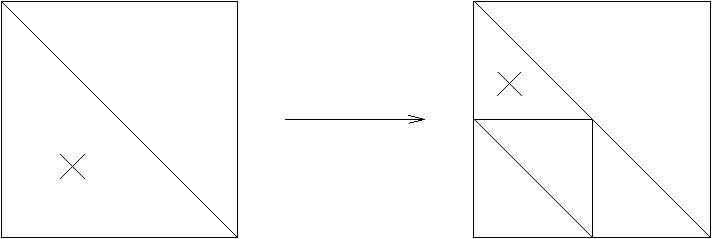
\includegraphics[height=2cm]{pictures/refine_irreg}
\end{center}
But, the obtained mesh is not regular. To avoid such irregular nodes,
also neighboring elements must be split (called green closure):
\begin{center}
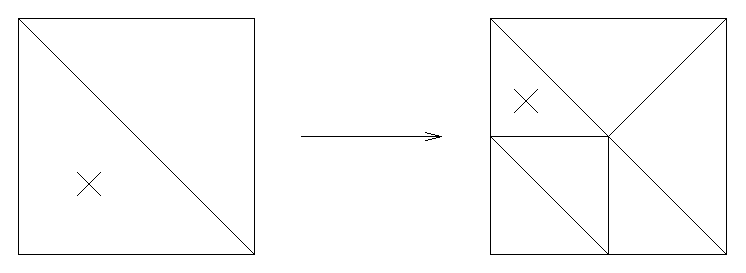
\includegraphics[height=2cm]{pictures/refine_reg}
\end{center}
If one continues to refine that way, the shape of the elements may get worse and worse:
\begin{center}
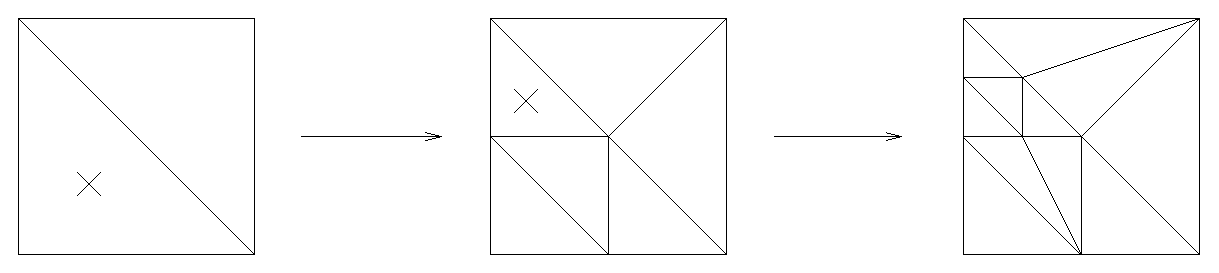
\includegraphics[height=2cm]{pictures/refinebad}
\end{center}
A solution is that elements of the green closure will not be further refined. 
Instead, remove the green closure, and replace it by red refinement. 
\begin{center}
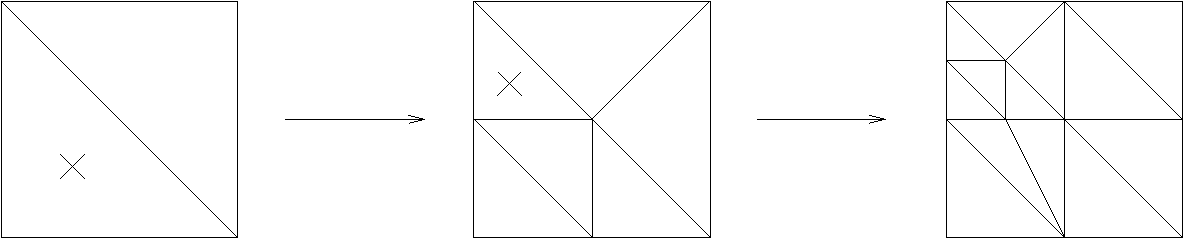
\includegraphics[height=2cm]{pictures/refinegood}
\end{center}


\bigskip
{\bf Marked edge bisection:} \newline
Each triangle has one marked edge. 
The triangle is only refined by cutting from the middle of the
marked edge to the opposite vertex. The marked edges of the new triangles
are the edges of the old triangle.

If there occurs an irregular node, then also the neighbor triangle must be refined.
\begin{center}
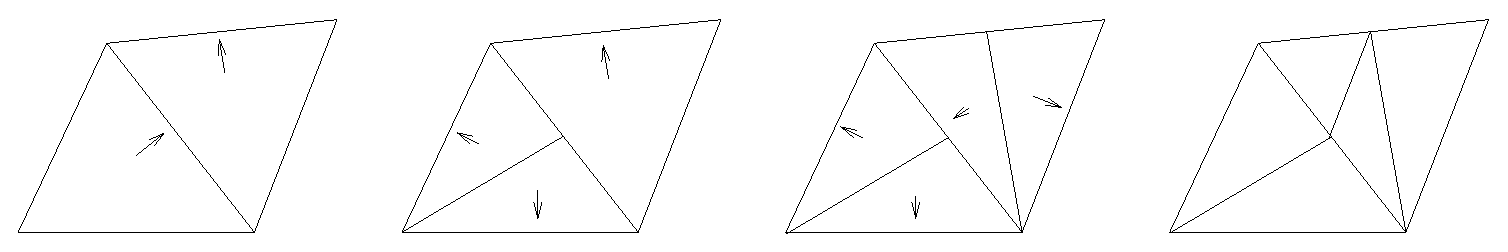
\includegraphics[height=2cm]{pictures/bisect}
\end{center}
To ensure finite termination, one has to avoid cycles in the initial mesh. 
This can be obtained by first sorting the edges (e.g., by length), end then, 
always choose the largest edges as marked edge.

\bigskip

Both of these refinement algorithms are also possible in 3D.

% \documentclass[12pt]{article}
% \usepackage{amsmath,amsthm,amssymb,a4wide}
% \usepackage[german,english]{babel}
% \usepackage{epsfig}
% \usepackage{latexsym}
% \usepackage{amssymb}
% % \usepackage{theorem}
% \usepackage{amsthm}
% % \usepackage{showkeys}

% \newcommand{\setR}{ {\mathbb R} }
% \newcommand{\setN}{ {\mathbb N} }
% \newcommand{\setZ}{ {\mathbb Z} }
% \newcommand{\eps}{\varepsilon}

% \newcommand{\beq}{\begin{equation}}
% \newcommand{\eeq}{\end{equation}}

% \newcommand{\opdiv}{\operatorname{div}}
% \newcommand{\opcurl}{\operatorname{curl}}
% \newcommand{\opdet}{\operatorname{det}}
% \newcommand{\optr}{\operatorname{tr}}
% \newcommand{\optrn}{\operatorname{tr}_n}
% \newcommand{\sfrac}[2]{ { \textstyle \frac{#1}{#2} } }

% \newcommand{\Zh}{\mathrm{Z}_h}
% \newcommand{\Ih}{\mathrm{I}_l}

% \newcommand{\leqc}{\preceq} 
% \newcommand{\geqc}{\succeq} 
% \newcommand{\eqc}{\simeq} 
% \newcommand{\ul}{\underline}

% \newtheorem{theorem}{Theorem}
% \newtheorem{definition}[theorem]{Definition}
% \newtheorem{lemma}[theorem]{Lemma}
% \newtheorem{remark}[theorem]{Remark}
% \newtheorem{example}[theorem]{Example}

% %
% %
% \setlength{\unitlength}{1cm}
% \sloppy 
% %

% \title{Equilibrated Residual Error Estimates}
% \author{Joachim Sch\"oberl}

% \begin{document}
% \maketitle

\section{Equilibrated Residual Error Estimates}

\subsection{General framework}
Equilibrated residual error estimators provide upper bounds for the discretization error in energy norm without any generic constant.
We consider the standard problem: find $u \in V := H_0^1(\Omega)$ such that
$$
\int_\Omega \lambda \nabla u \cdot \nabla v = \int_\Omega f v \qquad \forall \, v \in V
$$
The left hand side defines the bilinear-form $A(\cdot, \cdot)$, the right hand side the linear-form $f(\cdot)$. We define a finite element sub-space $V_h \subset V$ of order $k$, and the finite element solution
$$
\text{find } u_h \in V_h: \quad A(u_h, v_h) = f(v_h) \qquad \forall \, v_h \in V_h.
$$
We assume that $f$ is element-wise polynomial of order $k-1$, and $\lambda$ is element-wise constant and positive.

\qquad

The residual $r(\cdot) \in V^*$ is 
$$
r(v) = f(v) - A(u_h, v) \qquad v \in V
$$
Since 
$$
\| u - u_h \|_A = \sup_{v \in V} \frac{A(u-u_h, v)}{\| v \|_A} = 
 \sup_{v \in V} \frac { r(v) }{\| v \|_A},
$$
we aim in estimating $\|r \|$ in the norm dual to $\| \cdot \|_A$, which is essentially the $H^{-1}$-norm. In general, the direct evaluation of this norm is not feasible.
Using the structure of the problem, we can represent the residual as
$$
r(v) = \sum_{T \in \mathcal{T}} \int_T r_T v + \sum_{E \in \mathcal{E}} \int_E r_E v,
$$
where $r_T$ and $r_E$ are given given as
$$
r_T = f_T + \opdiv \lambda_T \nabla u_{h|T}  \qquad \text{and} \qquad
r_E = \left[  \lambda \frac{\partial u_h} {\partial n}  \right]_E
$$
The element-residual $r_T$ is a polynomial of order $k-1$ on the element $T$, and the edge residual (the normal jump) is a polynomial of order $k-1$ on the edge $E$. 

The {\em residual error estimator} estimates the residual in terms of weighted $L_2$-norms:
$$
\| r \|^2 \eqc \eta^{res}(u_h, f)^2 := \sum_T \frac{ h_T^2}{\lambda_T}  \| r_T \|_{L_2(T)}^2 + \sum_E \frac{ h_E }{\lambda_E} \| r_E \|_{L_2(E)}^2
$$
Here, $\lambda_E$ is some averaging of the coefficients on the two elements containing the edge~$E$. The equivalence holds with constants depending on the shape of elements, the relative jump of the coefficient, and the polynomial order $k$.


The {\em equilibrated residual error estimator} $\eta^{er}$ is defined in terms of the same data $r_T$ and $r_E$. It satisfies
\begin{eqnarray*}
\| u - u_h \|_A & \leq & \eta^{er} \qquad \text{reliable with constant 1} \\
\| u - u_h \|_A & \geq & c \, \eta^{er} \qquad \text{efficient with a generic constant $c$} \\
\end{eqnarray*}
The lower bound depends on the shape of elements and the coefficient $\lambda$, but is robust with respect to the polynomial order $k$.

The main idea is the following: Instead of calculating the $H^{-1}$-norm of $r$, we compute a lifting $\sigma^\Delta$ such that $\opdiv \sigma^\Delta = r$, and calculate the $L_2$-norm of $\sigma^\Delta$. Since $r$ is not a regular function, the equation must be posed in distributional form:
$$
\int_\Omega \sigma^\Delta \cdot \nabla \varphi = - r(\varphi) \qquad \forall \, \varphi \in V
$$
Then, the residual can be estimated without envolving any generic constant:
\begin{eqnarray*}
\| r \|_{A^\ast} & = & \sup_{v \in V} \frac{r(v)}{\| v \|_A} = \sup_v \frac{\int \sigma^\Delta \cdot \nabla v }{\|v \|_A} \\
&= & \sup_v \frac{\int \lambda^{-1/2} \sigma^\Delta \cdot \lambda^{1/2} \nabla v }{\|v \|_A}
\leq \sup_v \frac{\sqrt{\int \lambda^{-1} |\sigma^\Delta|^2}  \sqrt{ \int \lambda |\nabla v|^2 } }{\|v \|_A}
= \| \sigma^\Delta \|_{L_2, 1/\lambda}
\end{eqnarray*}
The norm $\| \sigma^\Delta \| := \int \lambda^{-1} | \sigma^\Delta|^2$ can be evaluated easily. 

Remark: The flux-postprocessing $\sigma := \lambda \nabla u_h + \sigma^\Delta$ provides a flux $\sigma \in H(\opdiv)$ such that $\opdiv \sigma = f$, i.e. the flux is in exact equilibrium with the source $f$. Thus the name.

\subsection{Computation of the lifting $\| \sigma^\Delta \|$}

The residual is a functional of the form
$$
r(v) = \sum_T (r_T, v)_{L_2(T)} + \sum_E (r_E, v)_{L_2(E)},
$$
where $r_T$ and $r_E$ are polynomials of order $k-1$. We search for $\sigma^\Delta$ which is element-wise a vector-valued polynomial of order $k$, and not continuous across edges. Element-wise integration by parts gives
$$
\int_\Omega \sigma \cdot \nabla \varphi = -\sum_T \int_T \opdiv \sigma_{|T} \varphi + \sum_E \int_E [\sigma \cdot n]_E \varphi.
$$
Thus $\opdiv \sigma = r$ in distributional sense reads as
$$
\opdiv \sigma{|T} = r_T \qquad \text{and} \qquad [\sigma \cdot n]_E = -r_E
$$
for all elements $T$ and edges $E$. We could now pose the problem 
$$
\min_{ \sigma \in P^k({\mathcal T})^2 \atop \opdiv \sigma = r} \| \sigma \|_{L_2, 1/\lambda}
$$
We minimize the weighted-$L_2$ norm since we want to find the smallest possible upper bound for the error. This is already a computable approach. 
But, the problem is global, and its solution is of comparable cost as the solution of the original finite element system.  The existence of a $\sigma$ such that $\opdiv \, \sigma = r$ also needs a proof.

We want to localize the construction of the flux. Local problems are associated with vertex-patches $\omega_V = \cup_{T : V \in T} T$. We proceed in two steps:
\begin{enumerate}
\item localization of the residual: $r = \sum_V r^V$
\item local liftings: find $\sigma^V$ such that $\opdiv \sigma^V = r^V$ on the vertex patch
\end{enumerate}
Then, for $\sigma := \sum \sigma^V$ there holds $\opdiv \sigma = r$

The localization is given by multiplication of the $P^1$ vertex basis functions (hat-functions) $\phi_V$:
$$
r^V(v) := r( \phi_V v)
$$
Since $\sum_V \phi_V = 1$, there holds $\sum r^V(\cdot) = r(\cdot)$. The localized residual has the same structure of element and edge terms:
$$
r^V(v) = \sum_{T \subset \omega_V} (r_T^V, v)_{L_2(T)} + \sum_{E \subset \omega_V} (r_E^V, v)_{L_2(E)},
$$
with 
$$
r_T^V = \phi_V r_T \qquad \text{and} \qquad r_E^V = \phi_V r_E
$$
The local residual vanishes on constants on the patch:
$$
r^V(1) = r(\phi_V \, 1) = A(u-u_h, \phi_V) = 0
$$
The last equality follows from the Galerkin-orthogonality. 

We give an explicit construction of the lifting $\sigma^V$ in terms of the Brezzi-Douglas-Marini (BDM) element. The $k^{th}$ order BDM element on a triangle is given by $V_T = [P^k]^2$ and the degrees of freedom:
\begin{enumerate}
\item[(i)] $\int_E \sigma\cdot n \, q_i$  with $q_i$ a basis for $ P^k(E)$
\item[(ii)] $\int_T \opdiv \sigma \, q_i$  with $q_i$ a basis for $ P^{k-1}(T) \cap L_2^0(T)$
\item[(iii)] $\int_T \sigma \cdot \opcurl q_i$  with $q_i$ a basis for $ P_0^{k+1}(T)$
\end{enumerate}
Exercise: Show that these dofs are unisolvent. Count dimensions, and prove that $[ \forall i: \psi_i(\sigma) =0 ] \Rightarrow \sigma = 0$.


Now, we give an explicit construction of equilibrated fluxes on a vertex patch. Label elements $T_1, T_2, \ldots T_n$ in a counter-clock-wise order. Edge $E_i$ is the  common edge between triangle $T_{i-1}$ and $T_i$ (with identifying $T_0 = T_n$). We define $\sigma$ by specifying the dofs of the BDM element:
\begin{enumerate}
\item
Start on $T_1$. We set $\sigma_n = -r^V_{E_1}$ on edge $E_1$. On the edge on the patch-boundary we set $\sigma_n = 0$, and on $E_2$ we set $\sigma_n = const$ such that $\int_{\partial T_1} \sigma_n = \int_{T_1} r^V_T$. We use the dofs of type (ii) to specify 
$\int_T \opdiv \sigma \, q = \int_T r_T^V q \; \forall q \in P^{k-1} \cap L_2^0(T)$. Together with get $\opdiv \sigma = r_T$. Dofs of type (iii) are not needed, and set 0. There holds
$$
\int_{E_2} \sigma_n = \int_{T_1} r^V_T - \int_{E_1} \sigma_n = \int_{T_1} r^V_{T_1} + \int_{E_1} r^V_{E_1}
$$
\item Continue with element $T_2$. On edge $E_2$ common with $T_1$ set $\sigma_n$ such that $[\sigma \cdot n]_{E_2} = r_{E_2}$. Otherwise, proceed as on $T_1$. Thus
$$
\int_{E_3} \sigma_n = \int_{T_1} r^V_{T_1} + \int_{E_1} r^V_{E_1} +\int_{T_2} r^V_{T_2} + \int_{E_2} r^V_{E_2} 
$$
\item Continue to element $T_n$. Observe that on $T_n$:
$$
\int_{E_1} \sigma_n = \sum_{i=1}^n \int_{T_i} r^V_{T_i} + \sum_{i=1}^n \int_{E_i} r^V_{E_i} = 0,
$$
which follows from $r^V(1) = 0$. Thus, also $[\sigma \cdot n]_{E_1} = r_{E_1}^V$ is satisfied.
\end{enumerate}

This explicit construction proves the existence of an equilibrated flux. Instead of this explicit construction, one may solve a local constrained optimization problem
$$
\min_{\sigma^V : \opdiv \sigma^V = r^V} \| \sigma \|_{L_2, \lambda^{-1}}
$$
This applies also for 3D. Furthoer notes
\begin{itemize}
\item mixed boundary conditions are possible
\item the efficiency for the h-FEM is shown by scaling arguments, and equivalence to the residual error estimator
\item efficiency is also proven to be robust with respect to polynomial order $k$, examples show overestimation less than 1.5
\end{itemize}


\bigskip \noindent 
{\bf Literature:}
\begin{enumerate}
\item 
D. Braess and J. Sch\"oberl.
\newblock  Equilibrated Residual Error Estimator for Maxwell's
Equations.
\newblock {\em Mathematics of Computation}, Vol 77(262), 651-672, 2008
\item 
D. Braess, V. Pillwein and J. Sch\"oberl: 
\newblock Equilibrated Residual Error Estimates are p-Robust. Computer
\newblock {\em Methods in Applied Mechanics and Engineering.} Vol 198,
1189-1197, 2009
\end{enumerate}



% \end{document}

\section{Non-conforming Finite Element Methods}
\label{sec_nonconforming}
In a conforming finite element method, one chooses a sub-space $V_h \subset V$, and defines the finite element approximation as
$$
\mbox{Find } u_h \in V_h: \qquad A(u_h, v_h) = f(v_h) \qquad \forall \, v_h \in V_{h}
$$
For reasons of simpler implementation, or even of higher accuracy, the 
conforming framework is often violated. Examples are:
\begin{itemize}
\item
The finite element space $V_h$ is not a sub-space of $V = H^m$. 
Examples are the non-conforming $P^1$ triangle, and the Morley element for
approximation of $H^2$.
\item
The Dirichlet boundary conditions are interpolated in the boundary vertices.
\item
The curved domain is approximated by straight sided elements
\item
The bilinear-form and the linear-form are approximated  by 
inexact numerical integration
\end{itemize}

\noindent
The lemmas by Strang are the extension of Cea's lemma to the 
non-conforming setting.


\subsubsection{The First Lemma of Strang}
In the first step, let $V_h \subset V$, but the bilinear-form and the linear-form are replaced by mesh-dependent forms 
$$
A_h(.,.): V_h \times V_h \rightarrow \setR
$$ 
and 
$$
f_h(.) : V_h \rightarrow \setR.
$$
We do not assume that $A_h$ and $f_h$ are defined on $V$. 
We assume that the bilinear-forms $A_h$ are uniformly coercive, i.e.,
there exists an $\alpha_1$ independent of the mesh-size such that
$$
A_h (v_h, v_h) \geq \alpha_1 \, \| v_h \|_V^2 \qquad \forall \, v_h \in V_h
$$
The finite element problem is defined as 
$$
\mbox{Find } u_h \in V_h: \qquad A_h (u_h, v_h) = f_h (v_h) \qquad \forall \, v_h \in V_h
$$

\begin{lemma}[First Lemma of Strang] Assume that
\begin{itemize}
\item $A(.,.)$ is continuous on $V$
\item $A_h(.,.)$ is uniformly coercive 
\end{itemize}
Then there holds
\begin{eqnarray*}
\| u - u_h \| & \leqc & \inf_{v_h \in V_h} \left\{
        \| u - v_h \| + \sup_{w_h \in V_h} \frac{|A(v_h, w_h) - A_h (v_h, w_h)|}{\| w_h \|} \right\} \\
        & & 
        + \sup_{w_h \in V_h} \frac{f(w_h) - f_h (w_h)}{\| w_h \|}
\end{eqnarray*}
\end{lemma}     
{\em Proof:} 
Choose an arbitrary $v_h \in V_h$, and set $w_h := u_h - v_h$.
We use the uniform coercivity, and the definitions of $u$ and $u_h$:
\begin{eqnarray*}
\alpha_1 \| u_h - v_h \|_V^2 & \leq & A_h (u_h - v_h, u_h - v_h) = A_h (u_h - v_h, w_h) \\
        & = & A(u-v_h, w_h) + [ A(v_h, w_h) - A_h(v_h, w_h) ] + [ A_h (u_h, w_h) - A(u, w_h)] \\
        & = & A(u-v_h, w_h) + [ A(v_h, w_h) - A_h(v_h, w_h) ] + [ f_h(w_h) - f(w_h)]
\end{eqnarray*}
Divide by $\| u_h - v_h \| = \| w_h \|$, and use the continuity of $A(.,.)$:
\begin{equation}
\label{equ_strang1a}
\| u_h - v_h \| \leqc \| u - v_h \| + \frac{|A(v_h, w_h) - A_h(v_h, w_h)|}{\| w_h  \|} + \frac{ | f(w_h) - f_h(w_h) | } { \| w_h \| }
\end{equation}

Using the triangle inequality, the error $\| u - u_h \|$ is bounded by
$$
\| u - u_h \| \leq \inf_{v_h \in V_h} \| u - v_h \| + \| v_h - u_h \|
$$
The combination with (\ref{equ_strang1a}) proves the result. 
\hfill $\Box$

\bigskip

{\bf Example:} Lumping of the $L_2$ bilinear-form: \newline
Define the $H^1$ - bilinear-form
$$
A(u,v) = \int_\Omega \nabla u \cdot \nabla v + \int_\Omega u v \, dx,
$$
and perform Galerkin discretization with $P^1$ triangles.
The second term leads to a non-diagonal matrix. 
The vertex integration rule
$$
\int_T v \, dx \approx \frac{|T|}{3} \sum_{\alpha = 1}^3 v(x_{T,\alpha})
$$
is exact for $v \in P^1$. We apply this integration rule for the term
$\int u v \, dx$:
$$
A_h(u,v) = \int \nabla u \cdot \nabla v + 
\sum_{T \in {\cal T}} \frac{|T|}{3} \sum_{\alpha = 1}^3 u(x_{T,\alpha}) v(x_{T,\alpha})
$$
The bilinear form is now defined only for $u, v \in V_h$.
The integration is not exact, since $u v \in P^2$ on each triangle.

Inserting the nodal basis $\varphi_i$, we obtain a diagonal matrix for
the second term:
$$
\varphi_i (x_{T,\alpha}) \varphi_j (x_{T,\alpha}) = 
        \left\{ \begin{array}{cl}
                1 & \mbox{for } x_i = x_j = x_{T,\alpha} \\
                0 & \mbox{else}
        \end{array}
        \right.
$$

To apply the first lemma of Strang, we have to verify the uniform coercivity
\begin{equation}
\label{equ_uniformell}
\sum_T \frac{|T|}{3} \sum_{\alpha = 1}^3 |v_h(x_{T,\alpha})|^2 \geq 
\alpha_1 \sum_T \int_T | v_h |^2 \, dx \qquad \forall \, v_h \in V_h,
\end{equation}
which is done by transformation to the reference element.
The consistency error can be estimated by
\begin{equation}
\label{equ_consist}
| \int_T u_h v_h \, dx - \frac{|T|}{3} \sum_{\alpha=1}^3 u_h(x_\alpha) v_h(x_\alpha) |
 \leqc h_T^2 \, \| \nabla u_h \|_{L_2(T)} \, \| \nabla v_h \|_{L_2(T)}
\end{equation}
Summation over the elements give
$$
A(u_h, v_h) - A_h (u_h, v_h) \leqc h^2 \| u_h \|_{H^1(\Omega)} \, \| v_h \|_{H^1(\Omega)}
$$
The first lemma of Strang proves that this modification of the bilinear-form
preserves the order of the discretization error:
\begin{eqnarray*}
\| u - u_h \|_{H^1} & \leqc & 
 \inf_{v_h \in V_h} \left\{
        \| u - v_h \|_{H^1} + \sup_{w_h \in V_h} \frac{|A(v_h, w_h) - A_h (v_h, w_h)|}{\| w_h \|_{H^1}} \right\} \\
 & \leqc & 
        \| u - I_h u \|_{H^1} + \sup_{w_h \in V_h} \frac{|A(I_h u, w_h) - A_h (I_h u, w_h)|}{\| w_h \|_{H^1}} \\
 & \leqc &  h \, \| u \|_{H^2} + \sup_{w_h \in V_h} \frac{h^2 \, \| I_h u \|_{H^1} \| w_h \|_{H^1}}{\| w_h \|_{H^1}} \\
 &  \leqc & h \, \| u \|_{H^2}
\end{eqnarray*}

A diagonal $L_2$ matrix has some advantages:
\begin{itemize}
\item It avoids oscillations in boundary layers (exercises!)
\item In explicit time integration methods for parabolic or hyperbolic
problems, one has to solve linear equations with the $L_2$-matrix. This
becomes cheap for diagonal matrices.
\end{itemize}

\subsubsection{The Second Lemma of Strang}

In the following, we will also skip the requirement $V_h \subset V$. 
Thus, the norm $\|.\|_V$ cannot be used on $V_h$, and it will be replaced by
mesh-dependent norms $\|.\|_h$. These norms must be defined for $V + V_h$.
As well, the mesh-dependent forms $A_h(.,.)$ and $f_h(.)$ are defined 
on $V + V_h$. We assume 
\begin{itemize}
\item uniform coercivity:
$$
A_h (v_h, v_h) \geq \alpha_1 \| v_h \|_h^2 \qquad \forall \, v_h \in V_h
$$
\item continuity:
$$
A_h (u, v_h) \leq \alpha_2 \| u \|_h \| v_h \|_h \qquad \forall \, u \in V + V_h, \; \forall \, v_h \in V_h
$$
\end{itemize}

The error can now be measured only in the discrete norm $\| u - u_h \|_{V_h}$.
\begin{lemma}
Under the above assumptions there holds
\begin{equation}
\label{equ_strang2}
\| u - u_h \|_h \leqc \inf_{v_h \in V_h} \| u - v_h \|_h +
         \sup_{w_h \in V_h} \frac{| A_h(u,w_h) - f_h(w_h) |}{\| w_h \|_h}
\end{equation}
\end{lemma}
{\em Remark}: The first term in (\ref{equ_strang2}) is the approximation
error, the second one is called consistency error. \\
{\em Proof:} Let $v_h \in V_h$. Again, set $w_h = u_h - v_h$, and
use the $V_h$-coercivity:
\begin{eqnarray*}
\alpha_1 \, \| u_h - v_h \|_h^2 & \leq & A_h (u_h - v_h, u_h - v_h) = A_h (u_h - v_h, w_h) \\
        & = & A_h (u-v_h, w_h) + [f_h(w_h) - A_h(u,w_h)]
\end{eqnarray*}
Again, divide by $\| u_h - v_h\|$, and use continuity of $A_h(.,.)$:
$$
\| u_h - v_h \|_h \leqc \| u - v_h \|_h + \frac{A_h(u,w_h) - f_h(w_h)}{\| w_h \|_h}
$$
The rest follows from the triangle inequality. \hfill $\Box$


\subsubsection{The non-conforming $P^1$ triangle}

The non-conforming $P^1$ triangle is also called the Crouzeix-Raviart element.

The finite element space generated by the non-conforming $P^1$ element
is
$$
V_h^{nc} := \{ v \in L_2 : v_{|T} \in P^1(T), \mbox{and }v \mbox{ is continuous in edge mid-points} \}
$$

The functions in $V_h^{nc}$ are not continuous across edges, and thus, 
$V_h^{nc}$ is not a sub-space of $H^1$. We have to extend the bilinear-form and
the norm in the following way:
$$
A_h (u,v) = \sum_{T \in {\cal T}} \int_T \nabla u \nabla v \, dx
        \qquad \forall \, u, v \in V + V_h^{nc}
$$
and
$$
\| v \|_h^2 := \sum_{T \in {\cal T}}  \| \nabla v \|_{L_2(T)}^2 \qquad \forall \, v \in V + V_h^{nc}
$$


We consider the Dirichlet-problem with $u = 0$ on $\Gamma_D$. 


We will apply the second lemma of Strang.

The continuous $P^1$ finite element space $V_h^c$ is a sub-space of 
$V_h^{nc}$. Let $I_h : H^2 \rightarrow V_h^c$ be the nodal interpolation
operator.

To bound the approximation term in (\ref{equ_strang2}), we use the
inclusion $V_h^c \subset V_h^{nc}$:
$$
\inf_{v_h \in V_h^{nc}} \| u - v_h \|_h \leq \| u - I_h u \|_{H^1} \leqc h \, \| u \|_{H^2}
$$


We have to bound the consistency term
\begin{eqnarray*}
r(w_h) & = & A_h(u,w_h) - f(w_h) \\
        & = & \sum_T \int_T \nabla u \nabla w_h - \sum_T \int_T f w_h \, dx \\
        & = & \sum_T \int_{\partial T} \frac{\partial u}{\partial n} w_h \, ds 
                - \sum_T \int_T (\Delta u + f) \, w_h \, ds \\
        & = & \sum_T \int_{\partial T} \frac{\partial u}{\partial n} w_h \, ds 
\end{eqnarray*}


Let $E$ be an edge of the triangle $T$. Define the mean value $\overline{w_h}^E$. 
If $E$ is an inner edge, then the mean value on the corresponding edge of
the neighbor element is the same. The normal derivative $\frac{\partial u}{\partial n}$ on the neighbor element is (up to the sign) the same.
If $E$ is an edge on the Dirichlet boundary, then the mean value is 0.
This allows to subtract edge mean values:

$$
r(w_h) = \sum_T \sum_{E \subset T} \int_E \frac{\partial u}{\partial n} (w_h - \overline{w_h}^E) \, ds
$$
Since $\int_E w_h - \overline{w_h}^E \, ds = 0$, we may insert the 
constant function $\frac{\partial I_h u}{\partial n}$ on each edge:
$$
r(w_h) = \sum_T \sum_{E \subset T} \int_E 
        \left(\frac{\partial u}{\partial n} - \frac{\partial I_h u}{\partial n} \right) (w_h - \overline{w_h}^E) \, ds
$$
Apply Cauchy-Schwarz on $L_2(E)$:
$$
r(w_h) = \sum_T \sum_{E \subset T} \| \nabla (u - I_h u) \|_{L_2(E)} \| w_h - \overline{w_h}^E \|_{L_2(E)}
$$

To estimate these terms, we transform to the reference element $\widehat T$, 
where we apply the Bramble Hilbert lemma. Let $T = F_T(\widehat T)$, and set
$$
\widehat u = u \circ F_T \qquad \widehat w_h = w_h \circ F_T
$$
There hold the scaling estimates
\begin{eqnarray*}
| w_h |_{H^1(T)} & \eqc & | \widehat w_h |_{H^1(\widehat T)} \\
\| w_h - \overline {w_h}^E \|_{L_2(E)} & \eqc & h_E^{1/2} \| \widehat w_h - \overline{\widehat w_h}^{\widehat E} \|_{L_2(\widehat E)} \\
| u |_{H^2(T)} & \eqc & h_T^{-1} |  \widehat u |_{H^2(\widehat T)} \\
\| \nabla (u - I_h u) \|_{L_2(E)} & \eqc & h_E^{-1/2} \| \nabla (\widehat u - \widehat I_h \widehat u) \|_{L_2(E)}
\end{eqnarray*}
On the reference element, we apply the Bramble Hilbert lemma, once for $w_h$, 
and once for $u$. The linear operator 
$$
L : H^1(\widehat T) \rightarrow L_2(\widehat E) :
 \widehat w_h \rightarrow  \widehat w_h - \overline {\widehat w_h}^{\widehat E}
$$
is bounded on $H^1(\widehat T)$ (trace theorem), and $L w = 0$ for $w \in P_0$,
thus
$$
\| \widehat w_h - \overline{\widehat w_h}^{\widehat E} \|_{L_2(\widehat E)}
\leqc | \widehat w_h |_{H^1(\widehat T)}
$$
Similar for the term in $u$: There is $\| \nabla (u - I_h u) \|_{L_2(E)} \leqc \| u \|_{H^2(T)}$, and $u - I_h u$ vanishes for $u \in P^1$. 

Rescaling to the element $T$ leads to
\begin{eqnarray*}
\| w_h - \overline{w_h}^E \|_{L_2(E)} & \leqc & h^{1/2} \, | w_h |_{H^1(T)} \\
\| \nabla (u - I_h u) \|_{L_2(E)} & \leqc & h^{1/2} \, | u |_{H^2(T)}
\end{eqnarray*}
This bounds the consistency term
$$
r(w_h) \leqc \sum_T h \, | u |_{H^2(T)} | w_h |_{H^1(T)} \leqc h \, \| u \|_{H^2(\Omega)} \, \| w_h \|_h.
$$
The second lemma of Strang gives the error estimate
$$
\| u - u_h \| \leqc h \, \| u \|_{H^2}
$$ 

There are several applications where the non-conforming $P^1$ triangle
is of advantage:
\begin{itemize}
\item
The $L_2$ matrix is diagonal (exercises)
\item
It can be used for the approximation of problems in fluid dynamics
described by the Navier Stokes equations (see later).
\item
The finite element matrix has exactly 5 non-zero entries in each row
associated with inner edges. That allows simplifications in the matrix
generation code.
\end{itemize}

% \documentclass[12pt]{article}
% \usepackage{amsmath,amsthm,amssymb,a4wide}
% \usepackage[german,english]{babel}
% \usepackage{epsfig}
% \usepackage{latexsym}
% \usepackage{amssymb}
% % \usepackage{theorem}
% \usepackage{amsthm}
% % \usepackage{showkeys}

% \newcommand{\setR}{ {\mathbb R} }
% \newcommand{\setN}{ {\mathbb N} }
% \newcommand{\setZ}{ {\mathbb Z} }
% \newcommand{\eps}{\varepsilon}

% \newcommand{\beq}{\begin{equation}}
% \newcommand{\eeq}{\end{equation}}

% \newcommand{\opdiv}{\operatorname{div}}
% \newcommand{\opcurl}{\operatorname{curl}}
% \newcommand{\opdet}{\operatorname{det}}
% \newcommand{\optr}{\operatorname{tr}}
% \newcommand{\optrn}{\operatorname{tr}_n}
% \newcommand{\sfrac}[2]{ { \textstyle \frac{#1}{#2} } }

% \newcommand{\Zh}{\mathrm{Z}_h}
% \newcommand{\Ih}{\mathrm{I}_l}

% \newcommand{\leqc}{\preceq} 
% \newcommand{\geqc}{\succeq} 
% \newcommand{\eqc}{\simeq} 
% \newcommand{\ul}{\underline}

% \newtheorem{theorem}{Theorem}
% \newtheorem{definition}[theorem]{Definition}
% \newtheorem{lemma}[theorem]{Lemma}
% \newtheorem{remark}[theorem]{Remark}
% \newtheorem{example}[theorem]{Example}

% %
% %
% \setlength{\unitlength}{1cm}
% \sloppy 
% %

% \title{hp - Finite Elements}
% \author{Joachim Sch\"oberl}

% \begin{document}
% % \selectlanguage{german}

% \maketitle

\section{hp - Finite Elements}

Let $V_{hp}$ be a $p$-th order finite element sub-space of $H^1$.
By scaling and Bramble-Hilbert technique one obtains the best-approxiamtion error estimate
$$
\inf_{v_{hp} \in V_{hp}} \| u - v_{hp} \|_{H^1}  \leq c h^{m-1} \| u \|_{H^m}
$$
for $m \leq p+1$. The constant $c$ depends on the order $p$. If $m$ is fixed, we do obtain reduction of the approximation error as we increase $p$. Next we develop methods to obtain so called $p$-version error estimates 
$$
\inf_{v_{hp} \in V_{hp}} \| u - v_{hp} \|_{H^1}  \leq c \left( \sfrac{h}{p} \right) ^{m-1} \| u \|_{H^m},
$$
where $c$ is independent of $h$ and $p$. This estimate proves also convergence of the $p$-version finite element method: One may fix the mesh, and increase the order $p$. 

A detailed analyis of local $H^m$ norms allows an optimal balance of
mesh-size $h$ and polynomial order $p$. This $hp$-version leads to
exponential convergence
$$
\inf_{v_{hp} \in V_{hp}} \| u - v_{hp} \|_{H^1}  \leq c e^{ -N^\alpha },
$$
where $N$ is the number of unknowns. 
 
We will prove the $p$-version estimate, but not the $hp$-result.

\subsection{Legendre Polynomials}
Orthogonal polynomials are important to construct stable basis 
functions for the $p$-FEM, as well as for error estimates.

Let $\Pi_n$ denote the space of polynomials up to order $n$. We write $\pi_n$ for 
a generic polynomial in $\Pi_n$, with a different value any time it appears.

Definition of Legendre polynomials via Rodrigues' formula:
$$
P_n(x) := \frac{1}{2^n n!} \frac{d^n}{dx^n} (x^2-1)^n.
$$
It is a polynomial of degree $n$. The first few Legendre polynomials are
\begin{eqnarray*}
P_0(x) & = & 1 \\
P_1(x) & = & x \\
P_2(x) & = & \sfrac{3}{2} x^2 - \sfrac{1}{2}
\end{eqnarray*}
$P_n$ is even if $n$ is even, and $P_n$ is odd if $n$ is odd.
Since $(x^2-1)^n = x^{2n} - n x^{2n-2} + \pi_{2n-4}$ (with proper
modification for small $n$) we have
\begin{equation}
\label{equ_leadingcoef}
P_n(x) = \frac{1}{2^n n!} \frac{ (2n)! }{ n! } x^n - \frac{n}{2^n n!} \frac{ (2n-2)!} {(n-2)!} x^{n-2} + \pi_{n-4}
\end{equation}
\begin{lemma} \label{lemma_ortho} There holds
\begin{equation} \label{equ_ortho}
\int_{-1}^1 P_n(x) P_m(x) \, dx = \frac{2}{2n+1} \delta_{n,m}.
\end{equation}
\end{lemma}
\begin{proof} W.l.o.g. let $n \leq m$. Multiple integration by parts gives
\begin{eqnarray*}
\lefteqn{ 2^{n+m} n! m! \int_{-1}^1 P_n(x) P_m(x) \, dx = 
\int_{-1}^1 \frac{d^n}{dx^n} (x^2-1)^n \frac{d^m}{dx^m} (x^2-1)^n  \, dx}
\\
& = & \int_{-1}^1 \frac{d^{n+1}}{dx^{n+1}} (x^2-1)^n \frac{d^{m-1}}{dx^{m-1}} (x^2-1)^m 
+ 
\left[ \frac{d^n}{dx^{n}} (x^2-1)^n \underbrace{ \frac{d^{m-1}}{dx^{m-1}} (x^2-1)^m}_{= 0 \text{ for } x \in \{ -1, 1\}} \right]_{-1}^1 \\
& = & \cdots \\
& = & \int_{-1}^1 \frac{d^{n+m}}{dx^{n+m}} (x^2-1)^n (x^2-1)^m \, dx
\end{eqnarray*} 
For $n < m$, the first factor of the integrand vanishes, and we have orthogonality. For $n = m$ this equals
\begin{eqnarray*}
2^{2n} (n!)^2 \| P_n \|_{L_2}^2 &= &\int_{-1}^1 (2n)! (x^2-1)^n \, dx = (2n)! \int_{-1}^1 (x-1)^n (x+1)^n \\
& = & -(2n)! \int_{-1}^1 \frac{n}{n+1} (x-1)^{n+1} (x+1)^{n-1} \\
& = & (2n)! \int_{-1}^1 \frac{ n (n-1) }{ (n+1) (n+2) } (x-1)^{n+2}(x+1)^{n-2} = ...  \\
& = & (2n)! \frac{n!} {2n (2n-1) \cdots (n+1)} \int_{-1}^1 (x-1)^{2 n} \, dx = (n!)^2 \frac{1}{2n+1} \, 2^{2n+1},
\end{eqnarray*}
which proves the scaling.
\end{proof}

Next we prove the 3-term recurrency, which can be used for efficient evaluation.
\begin{lemma} \label{lemma_threeterm} There holds
\begin{equation} \label{equ_threeterm}
(n+1) P_{n+1} (x) = (2n+1) x P_n(x) - n P_{n-1}(x).
\end{equation}
\end{lemma}
\begin{proof} Set $r(x) = (n+1) P_{n+1} (x) - (2n+1) x P_n(x) + n P_{n-1}(x)$.
Using (\ref{equ_leadingcoef}), we see that the leading coefficients cancel, 
and thus $r \in \Pi_{n-2}$. From Lemma~\ref{lemma_ortho} we get for 
any $q \in \Pi_{n-2}$
$$
\int_{-1}^1 r(x) q(x) \, dx = (n+1) \int_{-1}^1 P_{n+1} \, q - (2n+1) \int_{-1}^1 P_n \underbrace{x q}_{\in \Pi_{n-1}} + n \int_{-1}^1 P_{n-1} \, q = 0,
$$
and thus $r = 0$. 
\end{proof} 

\begin{lemma} \label{lemma_sturmliouville} Legendre polynomials satisfy the Sturm-Liouville differential equation
$$
\frac{d}{dx} \big[ (x^2-1) \frac{d}{dx} P_n(x) \big] = n (n+1) P_n(x)
$$
\end{lemma} 
\begin{proof} Both sides are in $\Pi_n$. We compare leading coefficients, for this set $P_n = a_n x^n + \pi_{n-2}$ (with $a_n =  \frac{1}{2^n n!} \frac{ (2n)! }{ n! }$).
\begin{eqnarray*}
lhs & = & \frac{d}{dx} \left[ (x^2-1) \frac{d}{dx} \left( a_n x^n + \pi_{n-2} \right) \right] \\
& = & \frac{d}{dx} \left[ (x^2-1) (a_n n x^{n-1} + \pi_{n-3}) \right] \\
& = & \frac{d}{dx} \left[ a_n n x^{n+1} + \pi_{n-1} \right] \\
& = & n (n+1) a_n x^n + \pi_{n-2}, 
\end{eqnarray*}
and we get the same leading coefficient for rhs. Furthermore, for $q \in \Pi_{n-1}$ there holds
\begin{eqnarray*}
\int_{-1}^1 lhs \, q & = &-\int_{-1}^1 (x^2-1) P_n^\prime q^\prime \, dx + \underbrace{ \left[ (x^2-1) P_n^\prime q \right]_{-1}^1 }_{= 0} \\
& = & \int_{-1}^1 P_n \underbrace{ \left( (x^2-1) q^\prime\right)^\prime}_{\in \Pi_{n-1}} \, dx - \left[ P_n (x^2-1) q^\prime \right]_{-1}^1 = 0,
\end{eqnarray*}
and the same for the rhs. Thus the identity is proven.
\end{proof}

Lemma~\ref{lemma_sturmliouville} implies that the Legendre polynomials are also orthogonal w.r.t. $(u^\prime, v^\prime)_{L_2, 1-x^2}$, i.e.
$$
\int_{-1}^1 (1-x^2) P_n^\prime P_m^\prime = n(n+1) \| P_n \|_{L_2}^2 \delta_{n,m}
$$


\subsection{Error estimate of the $L_2$ projection}
Since polynomials are dense in $L_2(-1,1)$, we get
$$
u = \sum_{n=0}^\infty a_n P_n
$$
with the generalized Fourier coefficients
$$
a_n = \frac{ (u, P_n)_{L_2} } { \| P_n \|^2_{L_2} },
$$
and
$$
\| u \|_{L_2}^2 = \sum_{n=0}^\infty a_n^2 \| P_n \|^2.
$$
Let $P_{L_2}^{\Pi_p}$ denote the $L_2$-projection onto $\Pi_p$. There holds
$$
P_{L_2}^{\Pi_p} u = \sum_{n=0}^p a_n P_n
$$
The projection error is
$$
\| u - P_{L_2}^{\Pi_p} u \|_{L_2}^2 = \sum_{n=p+1}^\infty a_n^2 \| P_n \|^2
$$
\begin{lemma} \label{lemma_l2est}  The $L_2$-projection error satisfies
\begin{equation}
\| u - P_{L_2}^{\Pi_p} u \|_{L_2(-1,1)} \leq \frac{1}{\sqrt{(p+1)(p+2)}} \, | u |_{H^1(-1,1)}
\end{equation}
\end{lemma}
\begin{proof} Since $P_n$ are orthogonal also w.r.t. $(u^\prime, v^\prime)_{L_2, 1-x^2}$,
there holds
$$
\| u^\prime \|_{L_2, 1-x^2}^2 = \sum_{n \in \setN} a_n^2 \, \| P_n^\prime \|_{1-x^2}^2,
$$
provided that $u$ is in $H^1$.
The projection error satisfies
\begin{eqnarray*}
\| u - P_{L_2}^{\Pi_p} u \|^2_{L_2} & = & \sum_{n > p} a_n^2 \| P_n \|^2_{L_2} 
 = \sum_{n > p} a_n^2 \frac{1}{n (n+1)} \| P_n^\prime \|^2_{1-x^2} \\
& \leq & \frac{1}{(p+1)(p+2)} \sum_{n > p} a_n^2 \|P_n^\prime \|^2_{1-x^2} 
\leq  \frac{1}{(p+1)(p+2)} \sum_{n \in \setN} a_n^2 \|P_n^\prime \|^2_{1-x^2} \\
& = & \frac{1}{(p+1)(p+2)} \| u^\prime \|_{1-x^2}^2 \\
\end{eqnarray*}
Finally, the result follows from 
$$
\int_{-1}^1 (1-x^2) (u^\prime)^2 \, dx \leq \int_{-1}^1 (u^\prime)^2 \, dx.
$$
\end{proof}
\newpage
Similar as in Lemma~\ref{lemma_sturmliouville} on shows also
$$
\frac{d^m}{dx^m} \big[ (x^2-1)^m \frac{d^m}{dx^m} P_n(x) \big] = (n+m)(n+m-1) \ldots (n-m+1) P_n(x)
$$
for $m \leq n$, and, as in Lemma~\ref{lemma_l2est}
$$
\| u - P_{L_2}^{\Pi_p} u \|_{L_2} \leq \sqrt{ \frac{ (p-m+1)! }{ (p+m+1)! } } | u |_{H^m}.
$$


\subsection{Orthogonal polynomials on triangles}
%
Orthogonal polynomials on tensor product elements are simply
constructed by tensorization. Orthogonal polynomials on simplicial
elements are more advanced. They are based on Jacobi polynomials:

For $\alpha, \beta > -1$, Jacobi polynomials are defined by 
$$
P_n^{(\alpha, \beta)}(x) := \frac{(-1)^n}{2^n n!} \frac{1}{w(x)} \frac{d^n}{dx^n} \big( w(x) (1-x^2)^n \big)
$$
with the weight function 
$$
w(x) = (1-x)^\alpha (1+x)^\beta.
$$
Jacobi polynomials are orthogonal w.r.t. the weighted inner product
$$
\int_{-1}^1 w(x) P_n^{(\alpha,\beta)}(x) P_m^{(\alpha, \beta)}(x) dx = \delta_{n,m} \frac{2^{\alpha+\beta+1}}{2n+\alpha+\beta+1} \frac{ \Gamma(n+\alpha+1) \, \Gamma (n+\beta+1) } { n! \Gamma (n+\alpha+\beta+1)}.
$$
Note that $P^{(0,0)}_n = P_n$.

Define the unit-triangle $T$ with vertices $(-1,0)$,  $(1,0)$ and $(0,1)$. 
\begin{lemma} [Dubiner basis] The functions
$$
\varphi_{i,j} (x,y) := P_i \big( \sfrac{x}{1-y} \big) (1-y)^i P_j^{(2i+1,0)} (2y-1)
\qquad i+j \leq p
$$ 
form an $L_2(T)$-orthogonal basis for $\Pi_p(T)$.
\end{lemma}
\begin{proof}
Note that $\varphi_{i,j} \in \Pi_{i+j}$. Substitution $\xi = \frac{x}{1-y}$ leads to
\begin{eqnarray*}
\lefteqn{ \int_T \varphi_{ij}(x,y) \varphi_{kl} (x,y) \, d(x,y) = } \\
& = & \int_0^1 \int_{-1+y}^{1-y} 
 P_i \big( \sfrac{x}{1-y} \big) (1-y)^i P_j^{(2i+1,0)} (2y-1)
 P_k \big( \sfrac{x}{1-y} \big) (1-y)^k P_l^{(2k+1,0)} (2y-1) \, dx dy \\
& = & \int_0^1 \int_{-1}^1 P_i(\xi) P_k(\xi) (1-y)^{i+k+1} P_j^{(2i+1,0)} (2y-1) P_l^{(2k+1,0)}(2y-1) \, d\xi dy \\
& = & \delta_{i,k} \| P_i \|_{L_2}^2 \int_0^1 (1-y)^{2i+1} P_j^{(2i+1,0)}(2y-1) P_l^{(2i+1,0)}(2y-1) \, dy \\
& = & C_{ij} \delta_{i,k} \delta_{j,l} 
\end{eqnarray*}
\end{proof}



\subsection{Projection based interpolation}

By means of the orthogonal polynomials one shows approximation error estimates
of the form
$$
\inf_{q \in \Pi_p(T)} \| u - q \|_{H^k(T)} \leq c p^{k-m} | u |_{H^m(T)} \qquad m \geq k,
$$
with $c \neq c(p)$, easily in 1D and tensor product elements, and also on $n$-dimensional simplices [Braess+Schwab: Approximation on simplices with respect to weighted Sobolev norms, J. Approximation Theory 103, 329-337 (2000)].
 
But, an interpolation operator to an $H^1$-conforming finite element space has to satisfy continuity constraints across element boundaries. We show that we get the same rate of convergence under these constraints.

\subsubsection{The 1D case}
Let $I=(-1,1)$. We define the operator $I_p : H^1(I) \rightarrow \Pi_p$ such that
\begin{eqnarray}
I_p u(x) & = & u(x) \qquad x \in \{ -1, 1 \}   \label{equ_projbased1} \\
\int_I (I_p u)^\prime q^\prime & = &  \int_I u^\prime q^\prime \qquad \forall \, q \in \Pi_{p,0}(I),   \label{equ_projbased2} 
\end{eqnarray}
where $\Pi_{p,0}(D) := \{ q \in \Pi_p(D) : q = 0 \text{ on } \partial D\}$.
This procedure is exactly a $p$-version Galerkin-method for the
Dirichlet problem.  Since boundary values are preserved, the
interpolation operator produces a globally continuous function.  The
operator $I_p$ is a kind of mixture of interpolation and projection,
thus the term {\em projection based interpolation} introduced by
Demkowicz has been established.

\begin{lemma}[Commuting diagram] There holds
$$
\Pi_{L_2}^{\Pi_{p-1}} u^\prime = (I_p u)^\prime 
$$
\end{lemma}
\begin{proof} The range of both sides is $\Pi_{p-1}$. We have to show that 
$(I_p u)^\prime$ is indeed the $L_2$-projection of $u^\prime$, i.e.
$$ 
\int_I (I_p u)^\prime q = \int_I u^\prime q \qquad \forall \, q \in \Pi_{p-1}.
$$
This holds since $\{ q^\prime : q \in \Pi_{p,0} \} = \{ q \in \Pi_{p-1} : \int q = 0 \}$ and (\ref{equ_projbased2}), and 
$$
\int_{-1}^1 (I_p u)^\prime \, 1 = (I_p u)(1)  - (I_p u)(-1) = u(1) - u(-1) = \int_{-1}^1 u^\prime \, 1.
$$
\end{proof}

The $H^1$-error estimate follows directly from the commuting diagram property:
$$
| u - I_p u |_{H^1(I)} = \| u^\prime - (I_p u)^\prime \|_{L_2} = 
\| u^\prime - P_{L_2}^{\Pi_{p-1}} u^\prime \|_{L_2} \leq \frac{c}{p^{m-1}} | u^\prime |_{H^{m-1}}.
$$
By the Aubin-Nitsche technique one obtains an extra $p$ for the $L_2$-error:
$$
\| u - I_p u \|_{L_2(I)} \leqc \frac{1}{p} | u - I_p u |_{H^1(I)} \leq \frac{1}{p^m} | u |_{H^m(I)}
$$
One also gets for $q \in \Pi_p$
$$
| u - I_p u |_{H^1} = | u-q - I_p (u-q) |_1 \leq || Id - I_p ||_{H^1\rightarrow H^1} \, | u - q |_{H^1}
$$

\subsubsection{Projection based interpolation on triangles}

We define the operator $I_p : H^2(T) \rightarrow \Pi_p(T)$ as follows:
\begin{eqnarray}
I_p u(x) & = & u(x) \qquad \forall \text{ vertices } x \\
\int_E \partial_\tau (I_p u) \partial_\tau q & = &  
\int_E \partial_\tau u  \partial_\tau q \qquad \forall \text{ edges } E, \; \forall \, q \in \Pi_{p,0}(E) \\
\int_T \nabla (I_p u) \nabla q & = & \int_T \nabla u \nabla q \qquad \forall \, q \in \Pi_{p,0}(T)
\end{eqnarray}
Note that $I_p u$ on the edge $E$ depends  only on $u|_E$, and thus the interpolant is
continuous across neighbouring elements. 



\begin{lemma}  \label{lemma_polext}  Let $v \in C(\partial T)$ such that $v|_E \in \Pi_p(E)$. Then there exists
an extension $\tilde v \in \Pi_p(T)$ such that $\tilde v|_{\partial T} = v$ and
$$
| \tilde v |_{H^1} \leq c \, | v |_{H^{1/2}(\partial T)},
$$
where $c$ is independent of $p$.
\end{lemma}
Major steps have been shown in exercises 5.2 and 6.6.
Note that the minimal-norm extension $\tilde v$ is the solution of the Dirichlet problem, i.e.
$$
\int_T \nabla \tilde v \nabla w = 0 \qquad \forall \, w \in \Pi_{p,0}
$$

\begin{theorem} [error estimate] There holds 
$$
| u - I_p u |_{H^1} \leqc
\inf_{q \in \Pi_p} | u - q |_{H^1(T)} + 
\sum_{E \subset \partial T} \frac{1}{\sqrt{p}} \inf_{q \in \Pi_p(E)} | u - q |_{H^1(E)}
\leqc 
\frac{1}{p^{m-1}} | u |_{H^m} 
$$
for $u \in H^m, m \geq 2$.  
\end{theorem}
\begin{proof} Let $u_p$ be the $|\cdot |_{H^1}$ best approximation to $u$, i.e.
$$
\int_T \nabla u_p \nabla v = \int_T \nabla u \nabla v \qquad \forall \, v \in \Pi_p,
$$
and, for uniqueness, mean values are preserved: $\int_T u_p = \int_T u$. There holds
$$
| u - u_p |_{H^1} \leq  \frac{c}{p^{m-1}} | u |_{H^m}.
$$

We apply the triangle inequality:
$$
| u - I_p u |_{H^1} \leq | u - u_p |_{H^1} + | u_p - I_p u |_{H^1}
$$
Since 
$$
\int_T \nabla u_p \nabla v = \int_T \nabla u \nabla v = \int_T \nabla I_p u  \nabla v
\qquad \forall \, v \in \Pi_{p,0}(T),
$$
we have that
$$
u_p - I_p u \; \bot_{H^1} \; \Pi_{p,0},
$$
i.e. $u_p - I_p u$ is solution of the Dirichlet problem with boundary values
$ (u_p - I_p u)|_{\partial T}$. Lemma~\ref{lemma_polext} implies that
$$
| u_p - I_p u |_{H^1(T)} \leqc | u_p - I_p u |_{H^{1/2}(\partial T)}
$$

We insert an $u$ on the boundary to obtain
\begin{eqnarray*}
| u - I_p u |_{H^1} & \leqc & | u - u_p |_{H^1(T)} + | u_p - I_p u |_{H^{1/2}(\partial T)} \\
& \leq & | u - u_p |_{H^1(T)} + | u_p - u |_{H^{1/2}(\partial T)} + | u - I_p u |_{H^{1/2}(\partial T)} \\
& \leq & | u - u_p |_{H^1(T)} + 
\| u - I_p u \|_{L_2(\partial T)}^{1/2} 
| u - I_p u |_{H^1(\partial T)}^{1/2}.
\end{eqnarray*}
In the last step we used that $H^{1/2}(\partial T) = [L_2, H^1]_{1/2}$ (i.e. the interpolation space).
Next, we observe that $I_p$ restricted to one edge $E$ is exactly the 1D operator. Using Aubin-Nitsche we get
\begin{eqnarray*}
| u - I_p u |_{H^1} & \leqc & | u - u_p |_{H^1(T)} + p^{-1/2} \| u - I_p u\|_{H^1(\partial T)} \\
& \leqc & | u  - u_p |_{H^1(T)} + \sum_E p^{1-m} \, | u |_{H^{m-1/2}(E)} \\
& \leqc & p^{1-m} | u |_{H^m(T)}
\end{eqnarray*}
In the last step we used the trace theorem.
\end{proof}


% \end{document}      

% \newpage


\chapter{Linear Equation Solvers}

The finite element method, or other discretization schemes, lead to
linear systems of equations
$$
A u = f. 
$$

The matrices are typically
\begin{itemize}
\item of large dimension $N$ ($10^4 - 10^8$ unknowns)
\item and sparse, i.e., there are only a few non-zero elements per row.
\end{itemize}

A matrix entry $A_{ij}$ is non-zero, if there exists a finite element connected
with both degrees of freedom $i$ and $j$.

A 1D model problem: Dirichlet problem on the interval. A uniform grid with
$n$ elements. The matrix is
$$
A = \left( \begin{array} {ccccc}
        2 & -1  \\
        -1 & 2 & -1 \\
         & \ddots & \ddots & \ddots \\
        & & -1 & 2 & -1 \\
        & & & -1 & 2 
        \end{array}
        \right)_{(n-1) \times (n-1)},
$$


A 2D model problem: Dirichlet problem on a unit-square. A uniform grid with $2 n^2$ triangles. The unknowns are enumerated lexicographically:
\begin{center}
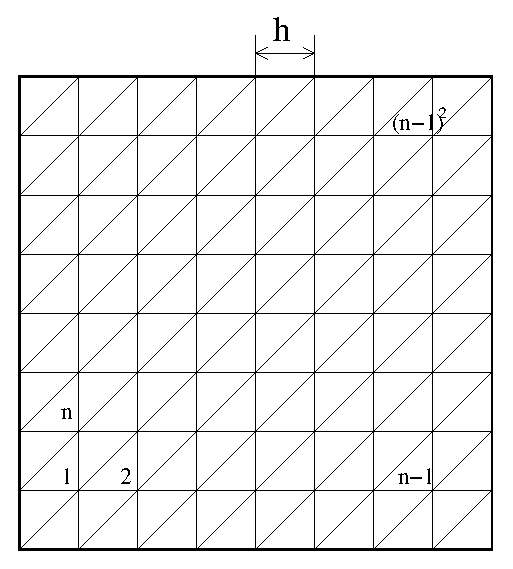
\includegraphics[width=4cm]{pictures/uniform_grid}
\end{center}

The FEM - matrix of dimension $N = (n-1)^2$ is
$$
A = \left( \begin{array} {ccccc}
        D & -I  \\
        -I & D & -I \\
         & \ddots & \ddots & \ddots \\
        & & -I & D & -I \\
        & & & -I & D 
        \end{array}
        \right)
\qquad \mbox{with} \qquad
D = \left( \begin{array} {ccccc}
        4 & -1  \\
        -1 & 4 & -1 \\
         & \ddots & \ddots & \ddots \\
        & & -1 & 4 & -1 \\
        & & & -1 & 4 
        \end{array}
        \right)_{(n-1) \times (n-1)},
$$
and the $(n-1) \times (n-1)$ identity matrix $I$.


\section{Direct linear equation solvers}
%
Direct solvers are factorization methods such as $LU$-decomposition,
or Cholesky factorization. They require in general $O(N^3) = O(n^6)$
operations, and $O(N^2) = O(n^4)$ memory. A fast machine can perform
about $10^9$ operations per second\footnote{time of writing was 2003}.  This corresponds to
%
\begin{center}
\begin{tabular}{cccc}
        n &$~\sim$N & time & memory \\
        \hline
        10 & $10^2$ & 1 ms & 80 kB \\
        100 & $10^4$ & 16 min & 800 MB \\
        1000 & $10^6$ & 30 years & 8 TB 
\end{tabular}
\end{center}

\bigskip

A band-matrix of (one-sided) band-width $b$ is a matrix with
$$
A_{ij} = 0 \qquad \mbox{for } |i-j| > b
$$
The $LU$-factorization maintains the band-width. $L$ and $U$ are triangular
factors of band-width $b$. A banded factorization method costs $O(N b^2)$
operations, and $O(Nb)$ memory. 
For the 1D example, the band-with is $1$. Time and memory are $O(n)$. For the
2D example, the band width is $O(n)$. The time complexity is $O(n^4)$, 
the memory complexity is $O(n^3)$.

This corresponds to
\begin{center}
\begin{tabular}{ccc}
        n & time & memory \\
        \hline
        10 & 10 $\mu$s & 8 kB \\
        100 & 0.1 s & 8 MB \\
        1000 & 16 min & 8 GB 
\end{tabular}
\end{center}
\bigskip

\subsubsection{Block-elimination methods}
By splitting the unknowns into two groups, we rewrite the equation $A u = f$ as
a block system
$$
\left( \begin{array}{cc}
        A_{11} & A_{12} \\
        A_{21} & A_{22} 
        \end{array} \right)
\left( \begin{array}{c}
        u_1 \\ u_2 
        \end{array} \right) =
\left( \begin{array}{c}
        f_1 \\ f_2 
        \end{array} \right).
$$
First, expressing $u_1$ from the first row gives
$$
u_1 = A_{11}^{-1} (f_1 - A_{12} u_2),
$$
and the Schur-complement equation to determine $u_2$
$$
(\underbrace{A_{22} - A_{21} A_{11}^{-1} A_{12}}_{=: S}) u_2 = f_2 - A_{21} A_{11}^{-1} f_1.
$$
This block-factorization is used in sub-structuring algorithms:
Decompose the domain into $m \times m$ sub-domains, each one containing
 $2 \frac{n}{m} \times \frac{n}{m}$ triangles. Split the unknowns into interior (I),
and coupling (C) unknowns. 
\begin{center}
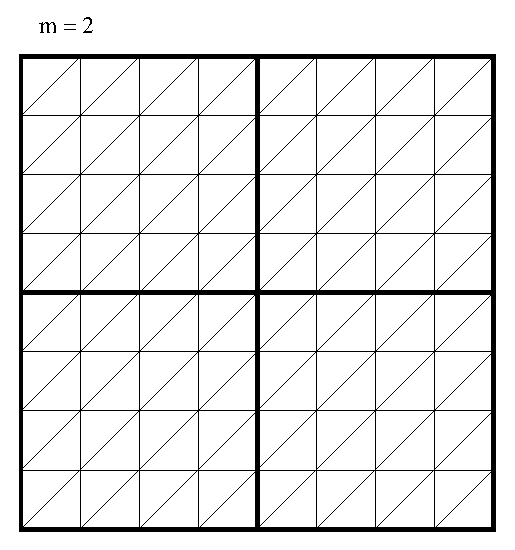
\includegraphics[width=4cm]{pictures/substructure}
\end{center}
The interior ones corresponding to different sub-domains have no connection in the
matrix. The block matrix is
$$
\left( \begin{array}{cc}
        A_I & A_{IC} \\
        A_{CI} & A_C 
        \end{array} \right) =
\left( \begin{array}{ccccc}
        A_{I,1} & & & A_{IC,1} \\
        & \ddots & & \vdots \\
        & & A_{I,m^2} & A_{IC,m^2} \\
        A_{CI,1} & \cdots & A_{CI,m^2} & A_C 
        \end{array} \right)
$$
Factorizing the block-diagonal interior block $A_I$ splits into $m^2$ independent
factorization problems. If one uses a banded factorization, the costs are
$$
m^2 \left( \frac{n}{m} \right)^4 = \frac{n^4}{m^2}
$$
Computing the Schur complement
$$
S = A_C - A_{CI} A_I^{-1} A_{IC} = A_C - \sum_{i=1}^{m^2} A_{CI,i} A_{I,i}^{-1} A_{IC,i}
$$
is of the same cost. The Schur complement is of size $m n$, and has band-width $n$. 
Thus, the factorization costs $O(m n^3)$. The total costs are of order
$$
\frac{n^4}{m^2} + m n^3
$$
Equilibrating both terms lead to the optimal number of sub-domains 
$m = n^{1/3}$, and to the asymptotic costs
$$
n^{3.33}
$$
If a parallel computer is used, the factorization of $A_I$ and the computation of
Schur complements can be performed in parallel.

\bigskip

The hierarchical sub-structuring algorithm, known as nested dissection, 
eliminates interior unknowns hierarchically:
\begin{center}
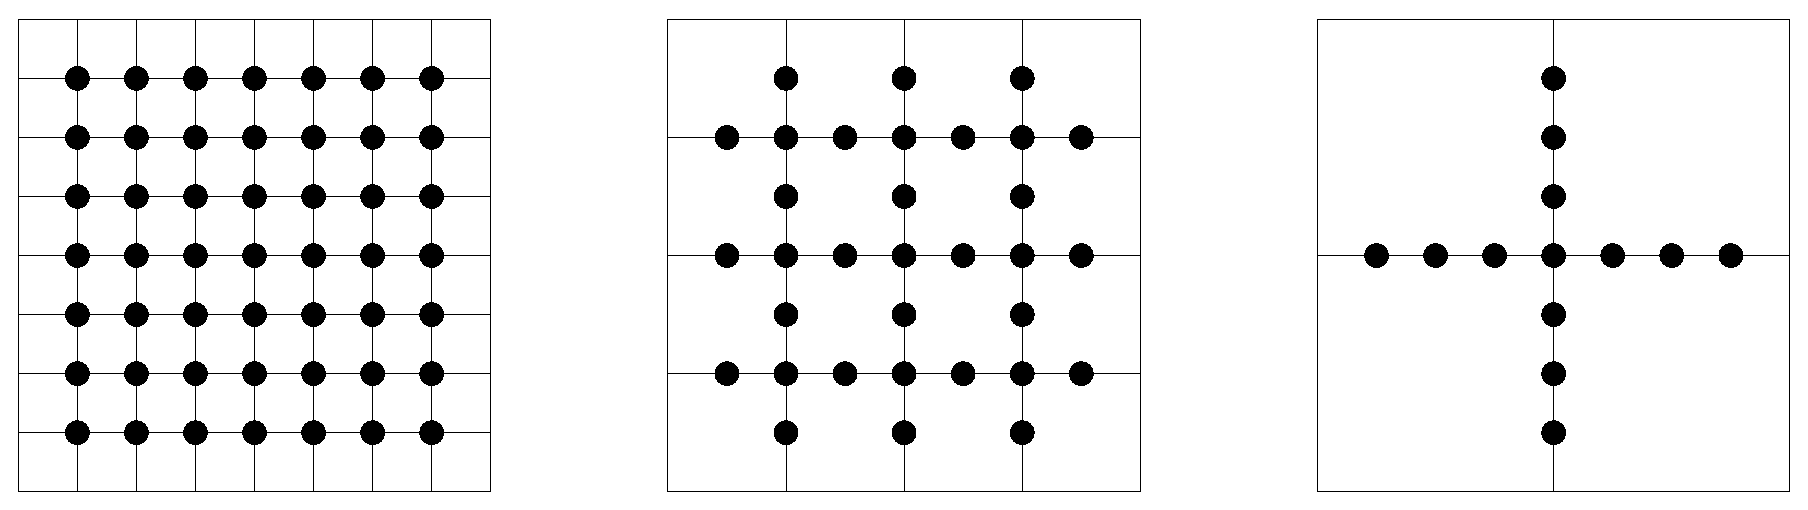
\includegraphics[width=12cm]{pictures/hierarchical}
\end{center}
Let $n = 2^L$. On level $l$, with $1 \leq l \leq L$, one has
$4^{l}$ sub-domains. Each sub-domain has $O(2^{L-l})$ unknowns.
The factorization of the inner blocks on level $l$ costs
$$
4^l \; (2^{L-l})^3 = 2^{3L - l}
$$
Forming the Schur-complement is of the same cost. The sum over all levels is
$$
\sum_{l=1}^L 2^{3L-l} = 2^{3L} \left( \frac{1}{2} + \frac{1}{4} + \ldots \right) \approx 2^{3L}
$$
The factorization costs are $O(n^3)$. Storing the matrices on each level costs
$$
4^l \; (2^{L-l})^2 = 2^{2L}.
$$
The total memory is $O(L \times 2^{2L}) = O(n^2 \, \log n)$. 


This corresponds to
\begin{center}
\begin{tabular}{ccc}
        n & time & memory \\
        \hline
        10 & 1 $\mu$s & 3 kB \\
        100 & 1 ms & 500 kB \\
        1000 & 1 s & 150 MB 
\end{tabular}
\end{center}
\bigskip

A corresponding sparse factorization algorithm for matrices arising
from unstructured meshes is based on  minimum degree
ordering. Successively, the unknowns with the least connections in the
matrix graph are eliminated.

In 2D, a direct method with optimal ordering is very efficient. In 3D, 
the situation is  worse for the direct solver. There holds $N = n^3$,
time complexity = $O(N^2)$, and memory = $O(N^{1.33})$.

\section{Iterative equation solvers}

Iterative equation solvers improve the accuracy of approximative solution by an
successive process. This requires in general much less memory, and, 
depending on the problem and on the method, may be (much) faster.

\subsubsection{The Richardson iteration}
A simple iterative method is the preconditioned Richardson iteration 
(also known as simple iteration, or Picard iteration):

\begin{quote}
start with arbitrary $u^0$ \newline
for $k = 0, 1, \ldots$ convergence \newline
\hspace*{1cm} $d^k = f - A u^k$ \newline
\hspace*{1cm} $w^k = C^{-1} d^k$ \newline
\hspace*{1cm} $u^{k+1} = u^k + \tau w^k$ 
\end{quote}

Here, $\tau$ is a damping parameter which may be necessary to ensure
convergence. 
The matrix $C$ is called a preconditioner. It should fulfill
\begin{enumerate}
\item $C$ is a good approximation to $A$
\item the matrix-vector multiplication $w = C^{-1} d$ should be cheap
\end{enumerate}
A simple choice is $C = \operatorname{diag} \, A$, the Jacobi preconditioner. The 
application 
of $C^{-1}$ is cheap. The quality of the approximation $C \approx A$
will be estimated below. The optimal choice for the first criterion would be
$C = A$. But, of course, $w = C^{-1} d$ is in general not cheap.


Combining the steps, the iteration can be written as
$$
u^{k+1} = u^k + \tau C^{-1} (f - A u^k)
$$
Let $u$ be the solution of the equation $A u = f$. 
We are interested in the behavior of the error $u^k - u$:
\begin{eqnarray*}
u^{k+1} - u & = & u^k - u + \tau C^{-1} (f - A u^k) \\
        & = & u^k - u + \tau C^{-1} (A u - A u^k) \\
        & = & (I - \tau C^{-1} A ) (u^k - u)
\end{eqnarray*}
We call the matrix 
$$
M = I - \tau C^{-1} A
$$
the {\it iteration matrix}. The error transition can be 
estimated by
$$
\| u^{k+1} - u \| \leq \| M \| \; \| u^k - u \|.
$$
The matrix norm is the associated matrix norm to some vector norm.
If $\rho := \| M \| < 1$, then the error is reduced. The error
after $k$ steps is
$$
\| u^k - u \| \leq \rho^k \| u^0 - u \|
$$
To reduce the error by a factor $\eps$ (e.g., $\eps = 10^{-8}$), one
needs
$$
N_{its} = \frac{\log \eps}{\log \rho}
$$
iterations.

We will focus on the symmetric ($A = A^T$) and positive definite ($u^T
A u > 0$ for $u \neq 0$) case (short: SPD). Then it makes sense to choose
symmetric and positive definite preconditioners $C = C^T$. Eigenvalue
decomposition allows a sharp analysis. Pose the generalized eigenvalue
problem
%
$$
A z = \lambda C z. 
$$
Let $(\lambda_i, z_i)$ be the set of eigen-pairs. The spectrum is $\sigma\{C^{-1} A\} = \{ \lambda_i \}$. The eigen-vectors $z_i$ are normalized to 
$$
\| z_i \|_C = 1
$$
The eigenvalues can are bounded from below and from above by the
Rayleigh quotient:
$$
\min_{v} \frac{v^T A v}{v^T C v} \leq \lambda_i \leq 
\max_{v} \frac{v^T A v}{v^T C v} 
$$ 

The ratio of largest to smallest eigen-value is the relative spectral 
condition number
$$
\kappa = \frac{\lambda_N}{\lambda_1}
$$

We will establish the spectral bounds
$$
\gamma_1 \, v^T C v \leq v^T A v \leq \gamma_2 \, v^T C v \qquad \forall \, v \in \setR^N,
$$
which allow to bound the eigenvalues
$$
\lambda_i \in [ \gamma_1, \gamma_2],
$$
and the condition number $\kappa \leq \frac{\gamma_2}{\gamma_1}$.


A vector $v$ can be expressed in terms of the eigen-vector basis $z_i$
as $v = \sum v_i e_i$. There holds
\begin{eqnarray*}
\| v \|_C^2 & = & \sum v_i^2 \\
\| v \|_A^2 & = & \sum \lambda_i v_i^2 
\end{eqnarray*}

\begin{lemma}
The iteration matrix $M$ can be bounded in $A$-norm and in $C$-norm:
$$
\| M \|_A \leq \sup_{\lambda \in [\gamma1, \gamma_2]} | 1 - \tau \lambda |
$$
$$
\| M \|_C \leq \sup_{\lambda \in [\gamma1, \gamma_2]} | 1 - \tau \lambda |
$$
\end{lemma}
{\em Proof:} Express $v = \sum v_i z_i$. Then
$$
M v = (I - \tau C^{-1} A) v = \sum v_i (I - \tau C^{-1} A) z_i
        = \sum v_i (1 - \tau \lambda_i) z_i
$$
The norm is
\begin{eqnarray*}
\| M v \|_A^2 & = & \sum \lambda_i v_i^2 (1-\tau \lambda_i)^2 \\
        & \leq & \sup_{i} (1-\tau \lambda_i)^2 \; \sum \lambda_i v_i^2 \\
        & \leq & \sup_{\lambda \in [\gamma_1, \gamma_2]} (1-\tau \lambda)^2 \; \| v \|_A^2
\end{eqnarray*}
and thus
$$
\| M \|_A = \sup_{v \in \setR^n} \frac{ \| M v \|_A } { \| v \|_A } 
        \leq \sup_{\lambda \in [\gamma_1, \gamma_2]} | 1 - \tau \lambda|.
$$ 
The proof is equivalent for $\|M\|_C$.
\hfill $\Box$


\bigskip


\begin{center}
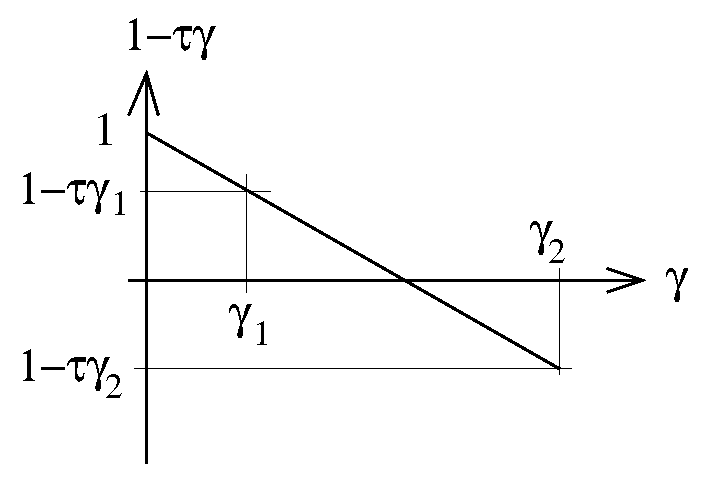
\includegraphics[height=3cm]{pictures/opttau}
\end{center}
The optimal choice of the relaxation parameter $\tau$ is such that
$$
1 - \tau \gamma_1  =  - (1-\tau \gamma_2), 
$$
i.e., 
$$
\tau = \frac{2}{\gamma_1 + \gamma_2}
$$
The convergence factor is
$$
1 - \tau \gamma_1 = \frac{\gamma_2 - \gamma_1}{\gamma_2 + \gamma_1}.
$$
Assume we knew sharp spectral bounds $\gamma_1 = \lambda_1$ and
$\gamma_2 = \lambda_N$. Then the convergence factor is
$$
\| M \| = \frac{\kappa-1}{\kappa+1} \approx 1 - \frac{2}{\kappa}
$$

The number of iterations to reduce the error by a factor $\eps$ is
$$
N_{its} = \frac{\log \eps}{\log \rho} \approx \frac {\log \eps}{-2/\kappa}
        = \log \eps^{-1} \, \frac{\kappa}{2}
$$



Take the 1D stiffness matrix of dimension $N \times N$:
$$
A = \left( \begin{array}{ccccc}
        2 & -1  \\
        -1 & 2 & -1 \\
        & \ddots & \ddots & \ddots \\
        & & -1 & 2 & -1 \\
        & & & -1 & 2 
        \end{array}
        \right),
$$
and the trivial preconditioner $C = I$. The eigen-vectors $z_i$ and 
eigen-values $\lambda_i$ are
\begin{eqnarray*}
z_{i} & = & \left(\sin \frac{i j \pi}{N+1} \right)_{j=1, \ldots N} \\
\lambda_i & = & 2 - 2 \cos (\frac{i \pi}{N+1})
\end{eqnarray*}
The extremal eigenvalues are
\begin{eqnarray*}
\lambda_1 & = & 2 - 2 \cos ( \frac{\pi}{N+1}) \approx \frac{\pi^2}{N^2} \\
\lambda_N & = & 2 - 2 \cos ( \frac{N \pi}{N+1} \approx 4 - \frac{\pi^2}{N^2}.
\end{eqnarray*}
The optimal damping is
$$
\tau = \frac{2}{\lambda_1+\lambda_N} = \frac{1}{2},
$$
and the convergence factor is
$$
\| M \| \approx 1 - \frac{2 \lambda_1}{\lambda_N} \approx 1 - \frac{2 \pi^2}{N^2}
$$

The number of iterations is
$$
N_{its} \eqc \log \eps^{-1} N^2
$$

\bigskip

For the 2D model problem with $N = (n-1)^2$, the condition number behaves like
$$
\kappa \eqc n^2.
$$

The costs to achieve a relative accuracy $\eps$ are
$$
N_{its} \times \mbox{Costs-per-iteration} 
\eqc \log \eps^{-1} n^2 N \eqc \log \eps^{-1} n^4
$$
The costs per digit are comparable to the band-factorization. The memory 
requirement is optimal $O(N)$.

\subsubsection{The gradient method}

It is not always feasible to find the optimal relaxation parameter $\tau$
a priori. The gradient method is a modification to the Richardson method
to find automatically the optimal relaxation parameter $\tau$:

The first steps are identic:
$$
d^k = f - A u^k \qquad w^k = C^{-1} d^k
$$
Now, perform the update
$$
u^{k+1} = u^k + \tau w^k
$$
such that the error is minimal in energy norm:
$$
\mbox{Find } \tau \mbox{ such that } \| u - u^{k+1} \|_A = \min !
$$
Although the error cannot be computed, this minimization is possible:

\begin{eqnarray*}
\| u - u^{k+1} \|_A^2 & = & \| u - u^k - \tau w^k \|_A^2 \\
        & = & (u-u^k)^T A (u-u_k) - 2 \tau (u-u^k)^T A w^k + \tau^2 (w^k)^T A w^k
\end{eqnarray*}
This is a convex function in $\tau$. It takes its minimum at
$$
0 = 2 (u-u^k)^T A w^k + 2 \tau_{opt}  (w^k)^T A w^k,
$$
i.e., 
$$
\tau_{opt} = \frac{ w^k A (u-u^k) } { (w^k)^T A w^k } = \frac{w^k d^k}{(w^k)^T A w^k}
$$

Since the gradient method gives optimal error reduction in energy norm, its
convergence rate can be estimated by the Richardson iteration with optimal
choice of the relaxation parameter:
$$
\| u - u^{k+1} \|_A \leq \frac{\kappa-1}{\kappa+1} \| u - u^k \|_A
$$

\subsubsection{The Chebyshev method}
We have found the optimal choice of the relaxation parameter for one
step of the iteration. If we perform $m$ iterations, the overall rate of convergence
can be improved by choosing variable relaxation parameters $\tau_1, \ldots \tau_m$.

The $m$-step iteration matrix is 
$$
M = M_m \ldots M_2 M_1 = (I - \tau_m C^{-1} A) \ldots (I - \tau_1 C^{-1} A).
$$
By diagonalization, the $A$-norm and $C$-norm are bounded by
$$
\| M \| \leq
 \max_{\lambda \in [\gamma_1, \gamma_N]} | (1-\tau_1 \lambda) \ldots (1-\tau_m \lambda) |
$$
The goal is to optimize $\tau_1, \ldots \tau_m$:
$$
\min_{\tau_1, \ldots \tau_m}
 \max_{\lambda \in [\gamma_1, \gamma_N]} | (1-\tau_1 \lambda) \ldots (1-\tau_m \lambda) |
$$
This is a polynomial in $\lambda$, of order $m$, and $p(0) = 1$:
\begin{equation}
\label{equ_polopt}
\min_{p \in P^m \atop p(0) = 1}
 \max_{\lambda \in [\gamma_1, \gamma_N]} | p(\lambda) |.
\end{equation}
This optimization problem can be solved explicitely by means of Chebyshev
polynomials. These are the polynomials defined by
$$
T_m(x) = \left\{ \begin{array}{cl}
         \cos (m \, \arccos (x))  & \; | x | \leq 1 \\
        \cosh (m \, \operatorname{arccosh} (x)) & \; | x | > 1 
        \end{array}
        \right.
$$
The $T_m$ fulfill the recurrence relation
\begin{eqnarray*}
T_0(x) & = & 1 \\
T_1(x) & = & x \\
T_{m+1}(x) & = & 2 x T_m(x) - T_{m-1}(x)
\end{eqnarray*}
The $T_m$ fulfill also
$$
T_m(x) = \frac{1}{2} \Big[ (x + \sqrt{x^2-1})^m + (x+\sqrt{x^2-1})^{-m} \Big]
$$


The optimum of (\ref{equ_polopt}) is 
$$
p(x) = \frac{T_m \left( \frac{2x-\gamma_1-\gamma_2}{\gamma_2-\gamma_1} \right)}
        {T_m \left( \frac{-\gamma_1-\gamma_2}{\gamma_2-\gamma_1} \right)}
        = C_m \; T_m \left( \frac{2x-\gamma_1-\gamma_2}{\gamma_2-\gamma_1} \right)
$$

The numerator is bounded by $1$ for the range $\gamma_1 \leq x \leq \gamma_2$.
The factor $C_m$ can be computed as
$$
C_m
        = \frac{2 c^m}{1+c^{2m}}
\qquad \mbox{with} \qquad
        c = \frac{\sqrt{\gamma_2} - \sqrt{\gamma_1}}{\sqrt{\gamma_2} + \sqrt{\gamma_1}}
$$
Using the condition number we have
$$
c \approx 1 - \frac{2}{\sqrt \kappa},
$$
and
$$
C_m \approx
( 1 - \frac{2}{\sqrt \kappa})^m
$$
Now, an error reduction by a factor of $\eps$ can be achieved in
$$
N_{its} \approx \log \eps^{-1} \sqrt{\kappa}
$$
steps. The original method by choosing $m$ different relaxation parameters 
$\tau_k$ is not a good choice, since
\begin{itemize}
\item it is not numerically stable
\item one has to know a priori the number of iterations 
\end{itemize}
The recurrence relation for the Chebyshev polynomials leads to a practicable
iterative method called Chebyshev iteration. 

\subsubsection{The conjugate gradient method}

The conjugate gradient algorithm automatically finds the optimal 
relaxation parameters for the best $k$-step approximation.



Let $p_0, p_1, \ldots$ be a finite sequence of $A$-orthogonal vectors, and set 
$$
V_k = \mbox{span} \{ p_0, \ldots p_{k-1} \}
$$

We want to approximate the solution $u$ in the linear manifold $u_0+ V_k$:
$$
\min_{v \in u_0 + V_k} \| u - v \|_A 
$$

We represent $u_k$ as
$$
u_k = u_0 + \sum_{l=0}^{k-1} \alpha_l p_l
$$
The optimality criteria are
$$
0 = (u-u_k, p_j)_A = (u - u_0 - \sum_{l=0}^{k-1} \alpha_l p_l, p_j)_A 
 \qquad   0 \leq j < k.
$$
The coefficients $\alpha_l$ follow from the $A$-orthogonality:
$$
\alpha_l = \frac{(u-u_0)^T A p_l}{p_l^T A p_l} = \frac{(f-A u_0)^T p_l}{p_l^T A p_l} 
$$
The $\alpha_l$ are computable, since the $A$-inner product was chosen.
The best approximations can be computed recursively:
$$
u_{k+1} = u_k + \alpha_k p_k
$$
Since $u_k - u_0 \in V_k$, and $p_k \bot_A V_k$, there holds
$$
\alpha_k = \frac{(f-A u_k)^T p_k}{p_k^T A p_k}.
$$


\bigskip

Any $k$-step simple iteration approximates the solution $u_k$ in the
manifold
$$
u_0 + {\cal K}_k(d_0)
$$
with the {\em Krylov space}
$$
{\cal K}_k(d_0) = \{ C^{-1} d_0, C^{-1} A C^{-1} d_0, \ldots , C^{-1} (A C^{-1})^{k-1} d_0 \}.
$$

Here, $d_0 = f - A u_0$ is the initial residual.
The conjugate gradient method computes an $A$-orthogonal basis of the
Krylov-space. The term {\em conjugate} is equivalent to $A$-orthogonal.

\begin{quote}
{\bf Conjugate Gradient Algorithm:} \newline
Choose $u_0$, compute $d_0 = f - A u_0$, set $p_0 = C^{-1} d_0$. \newline
for $k = 0, 1, 2, \ldots$ compute
\begin{eqnarray*}
\alpha_k & = & \frac{d_k^T p_k}{p_k^T A p_k} \\
u_{k+1} & = & u_k + \alpha_k \, p_k \\
d_{k+1} & = & d_k - \alpha_k \, A p_k \\
\beta_k & = & -\frac{d_{k+1}^T C^{-1} A p_k}{p_k^T A p_k} \\
p_{k+1} & = & C^{-1} d_{k+1} + \beta_k p_k
\end{eqnarray*}
\end{quote}

\begin{remark} In exact arithmetic, the conjugate gradient algorithm 
terminates at a finite number of steps $\overline{k} \leq N$.
\end{remark}



\begin{theorem} The conjugate gradient algorithm fulfills for $k \leq \overline{k}$
\begin{enumerate}
\item
The sequence $p_k$ is $A$-orthogonal. It spans the Krylov-space ${\cal K}_k(d_0)$
\item
The $u_k$ minimizes
$$
\min_{v \in u_0 + {\cal K}_k(d_0)} \| u - v \|_A
$$
\item
There holds the orthogonality
$$
d_k^T p_l = 0 \qquad \forall \, l < k
$$
\end{enumerate}
\end{theorem}
\noindent
{\em Proof:} Per induction in $k$. We assume 
\begin{eqnarray*}
p_k^T A p_l & = & 0 \qquad \forall \; l < k \\
d_k^T p_l & = & 0 \qquad \forall \; l < k 
\end{eqnarray*}
This is obvious for $k = 0$. We prove the property for $k+1$:
For $l < k$ there holds
$$
d_{k+1}^T p_l = (d_k - \alpha_k A p_k)^T p_l = 
        d_k^T p_l - \alpha_k p_k^T A p_l = 0
$$
per induction. For $l = k$ there is
$$
d_{k+1}^T p_k = (d_k-\alpha_k A p_k)^T p_k = d_k^T p_k - \frac{d_k^T p_k}{p_k^T A p_k}\; p_k^T A p_k = 0.
$$ 
Next, prove the $A$-orthogonality of the $p_k$. For $l < k$ we have
\begin{eqnarray*}
(p_{k+1}, p_l)_A & = & (C^{-1} d_{k+1} + \beta_k p_k, p_l)_A \\
        & = & d_{k+1}^T C^{-1} A p_l
\end{eqnarray*}
There is
$$
C^{-1} A p_l \in \mbox{span} \{ p_0, \ldots p_k \}, 
$$
and $d_{k+1}^T p_j = 0$ for $j \leq k$. For $l = k$ there is
\begin{eqnarray*}
(p_{k+1}, p_k)_A & = & (C^{-1} d_{k+1} + \beta_k p_k, p_k)_A \\
        & = & (C^{-1} d_{k+1}, p_k)_A   
                -\frac{d_{k+1}^T C^{-1} A p_k}{p_k^T A p_k} \; p_k^T A p_k  = 0
\end{eqnarray*}
\hfill $\Box$

The coefficients $\alpha_k$ and $\beta_k$ should be computed by the equivalent,
and numerically more stable expressions
$$
\alpha_k = \frac{d_k^T C^{-1} d_k}{p_k^T A p_k} \qquad
\beta_k = \frac{d_{k+1}^T C^{-1} d_{k+1}}{d_k^T C^{-1} d_k}.
$$

\begin{theorem} The conjugate gradient iteration converges with the rate
$$
\| u - u_k \|_A \leq  \left( \frac{\sqrt{\kappa} - 1}{\sqrt{\kappa}+1} \right)^k
$$
\end{theorem}
{\em Proof:} The conjugate gradient gives the best approximation in the
Krylov space. Thus, it can be bounded by the Chebyshev method leading to that rate.


\bigskip

The conjugate gradient iteration is stopped as soon as a convergence 
criterion is fulfilled. Ideally, one wants to reduce the error in the energy
norm by a factor $\eps$:
$$
\| u - u_k \|_A \leq \eps \, \| u - u_0 \|_A
$$
But, the energy error cannot be computed. We rewrite
$$
\| u - u_k \|_A^2 = \| A^{-1} (f - A u_k) \|_A^2 = \| A^{-1} d_k \|_A^2
= d_k^T A^{-1} d_k
$$
If $C$ is a good approximation to $A$, then also $C^{-1}$ is one to $A^{-1}$. 
The error can be approximated by 
$$
d_k^T C^{-1} d_k.
$$
This scalar is needed in the conjugate gradient iteration, nevertheless.

\bigskip

For solving the 2D model problem with $C = I$, the time complexity is
$$
\log \eps^{-1} \, N \sqrt{\kappa} = \log \eps^{-1} \, n^3
$$
The costs for one digit are comparable to the recursive sub-structuring algorithm. In 3D, the conjugate gradient method has better time complexity. 


\section{Preconditioning}

In the following, let the symmetric and positive definite matrix
$A$ arise from the finite element discretization of the $H^1$-elliptic 
and continuous bilinear-form $A(.,.)$.
We construct preconditioners $C$ such that the preconditioning action
$$
w = C^{-1} \times d
$$
is efficiently computable, and estimate the spectral bounds
$$
\gamma_1 \, u^T C u \leq u^T A u \leq \gamma_2 \, u^T C u \qquad
\forall \, u \in \setR^N
$$


The analysis of the preconditioner is performed in the finite element
framework. For this, define the Galerkin isomorphism
$$
G : \setR^N \rightarrow V_h : \underline u \rightarrow u = \sum u_i \varphi_i,
$$
where $\varphi_i$ are the fe basis functions. Its dual is 
$$
G^\ast : V_h^\ast \rightarrow \setR^N : d(\cdot) \rightarrow (d(\varphi_i))_{i=1,\ldots, N}.
$$
To distinguish vectors and the  corresponding finite element functions,
we write vectors $\underline u \in \setR^N$ with underlines (when necessary).

The evaluation of the quadratic form is
$$
\ul u^T A \ul u = A(G \ul u, G \ul u) \eqc \| G \ul u \|_{H^1}^2
$$

\subsubsection{The Jacobi Preconditioner}

The Jacobi preconditioner $C$ is
$$
C = \mbox{diag} \, A.
$$
The preconditioning action is written as
$$
C^{-1} \times \underline d = 
\sum_{i=1}^N e_i (e_i^T A e_i)^{-1} e_i^T \; \underline d
$$
Here, $e_i$ is the $i^{th}$ unit-vector. Thus, $e_i^T A e_i$ gives the
$i^{th}$ diagonal element $A_{ii}$ of the matrix, which is
$$
A_{ii} = A(\varphi_i, \varphi_i) \eqc \| \varphi_i \|_{H^1}^2.
$$
%
The quadratic form generated by the preconditioner is
$$
\ul {u} ^T C \ul u = \sum_{i=1}^N u_i^2 \| \varphi_i \|_A^2
 \eqc \sum_{i=1}^N u_i^2 \| \varphi_i \|_{H^1}^2
$$

\begin{theorem} \label{theo_jacobi} 
Let $h$ be the minimal mesh-size of a shape-regular
triangulation. Then there holds
\begin{equation}\label{equ_jacobi}
h^2 \; \ul u^T C \ul u \leqc u^T A u \leqc \, u^T C u
\end{equation}
\end{theorem}
{\em Proof:} We start to prove the right inequality
$$
\ul u^T A \ul u = \| \sum_{i} u_i \varphi_i \|_A^2 \leqc 
\ul u^T C \ul u = \sum_i u_i^2 \| \varphi_i \|_A^2.
$$
We define the interaction matrix $O$ with entries
$$
O_{ij} = \left\{ \begin{array} {cl}
        1 & A(\varphi_i, \varphi_j) \neq 0 \\
        0 & \mbox{else} 
        \end{array} \right.
$$
On a shape regular mesh, only a (small) finite number of basis functions have
overlapping support. Thus, $O$ has a small number of entries $1$ per row.
There holds
\begin{eqnarray*}
\| \sum_i u_i \varphi_i \|_A^2 & = &
        \sum_i \sum_j u_i u_j A(\varphi_i, \varphi_j) \\
        & = & \sum_i \sum_j u_i u_j O_{ij} A(\varphi_i, \varphi_j)  \\
        & \leq & \sum_i \sum_j (u_i \| \varphi_i \|_A)  O_{ij} (u_j  \| \varphi_j \|_A) \\
        & \leq & \rho (O) \sum_i   ( u_i \|\varphi_i \|_A)^2 \\
        & = & \rho(O) \ul u^T C \ul u.
\end{eqnarray*}
The spectral radius $\rho(O) = \max_{x \in \setR^N} \frac{x^T O x}{\|x\|^2}$ 
is bounded by the (small) finite row-sum norm of $O$.

The other estimate is proven element by element. Note that
$$
\ul u^T A \ul u \eqc \| u \|_{H^1(\Omega)}^2 = \sum_T \| \sum_i u_i \varphi_i \|_{H^1(T)}^2
$$
and
$$
\ul u^T C \ul u \eqc \sum_i \| u_i \varphi_i \|_{H^1(\Omega)}^2
= \sum_T  \sum_i \| u_i \varphi_i \|_{H^1(T)}^2.
$$
We prove the inequality for each individual element.
The triangle $T$ has diameter $h_T$. On $T$, we expand $u$ in terms of
the element shape functions $\varphi_\alpha$, namely
$u|_T = \sum_{\alpha=1}^3 u_\alpha \varphi_\alpha$. We transform to the
reference element $\widehat T$:
\begin{eqnarray*}
\| \sum_\alpha u_\alpha \varphi_\alpha \|_{H^1(T)}^2 & = &
\| \sum_\alpha u_\alpha \varphi_\alpha \|_{L_2(T)}^2 +
\| \nabla \sum_\alpha u_\alpha \varphi_\alpha \|_{L_2(T)}^2 \\
        & \eqc & 
h_T^2 \, \| \sum_\alpha u_\alpha \widehat \varphi_\alpha \|_{L_2(\widehat T)}^2 +
\| \nabla \sum_\alpha u_\alpha \widehat \varphi_\alpha \|_{L_2(\widehat T)}^2 \\
& \geq & 
h_T^2 \, \| \sum_\alpha u_\alpha \widehat \varphi_\alpha \|_{L_2(\widehat T)}^2
\end{eqnarray*}
and
\begin{eqnarray*}
 \sum_\alpha\| u_\alpha \varphi_\alpha \|_{H^1(T)}^2 & = &
\sum_\alpha \|  u_\alpha \varphi_\alpha \|_{L_2(T)}^2 +
\sum_\alpha \| \nabla  u_\alpha \varphi_\alpha \|_{L_2(T)}^2 \\
        & \eqc & 
h_T^2 \, \sum_\alpha \|  u_\alpha \widehat \varphi_\alpha \|_{L_2(\widehat T)}^2 +
\sum_\alpha \| \nabla  u_\alpha \widehat \varphi_\alpha \|_{L_2(\widehat T)}^2 \\
& \leqc & \sum_\alpha \|  u_\alpha \widehat \varphi_\alpha \|_{L_2(\widehat T)}^2 
\end{eqnarray*}
Both, $(u)_\alpha \rightarrow \| \sum_\alpha u_\alpha \widehat \varphi_\alpha \|_{L_2(\widehat T)}$ and
$u \rightarrow \left\{ \sum_\alpha \|  u_\alpha \widehat \varphi_\alpha \|_{L_2(\widehat T)}^2 \right\}^{1/2}$ are norms on $\setR^3$. Since all norms in $\setR^3$ are equivalent, we have
\begin{equation}  \label{equ_estjact}
 \sum_\alpha\| u_\alpha \varphi_\alpha \|_{H^1(T)}^2 \leqc h_T^{-2}
\| \sum_\alpha u_\alpha \varphi_\alpha \|_{H^1(T)}^2.
\end{equation}
By summing over all elements and choosing $h = \min h_T$, we have proven
the left inequality of (\ref{equ_jacobi}).
\hfill $\Box$

\bigskip

{\em Remark:} Inequality (\ref{equ_estjact}) is sharp. To prove this,
choose $u_\alpha = 1$. 

\subsubsection{Block-Jacobi preconditioners}

Instead of choosing the diagonal, one can choose a block-diagonal of $A$, e.g.,
\begin{itemize}
\item In the  case of systems of PDEs, choose blocks consisting of all 
degrees of freedom sitting in one vertex. E.g., mechanical deformations
$(u_x, u_y, u_z)$.
\item For high order elements, choose blocks consisting of all degrees of 
freedom associated to the edges (faces, inner) of the elements.
\item On anisotropic tensor product meshes, choose blocks consisting of 
unknowns in the short direction
\item Domain decomposition methods: Choose blocks consisting of the
unknowns in a sub-domain
\end{itemize}

Decompose the unknowns into $M$ blocks, the block $i$ has dimension $N_i$. 
Define the rectangular embedding matrices
$$
E_i \in \setR^{N \times N_i} \qquad i = 1, \ldots, M.
$$
$E_i$ consists of $N_i$ unit vectors corresponding to the unknowns in the
block $i$. Each $\ul u \in \setR^N$ can be uniquely written as
$$
\ul u = \sum_{i=1}^M E_i \ul u_i \qquad \mbox{with} \quad \ul u_i \in \setR^{N_i}
$$
The diagonal blocks are
$$
A_i = E_i^T A E_i \qquad i = 1, \ldots, M.
$$
The block Jacobi preconditioner is
$$
C^{-1} \times \ul d = \sum_{i=1}^M E_i A_i^{-1} E_i^T \, \ul d
$$
%
The quadratic form induced by $C$ can be written as
$$
\ul u^T C \ul u = \sum_i \ul u_i^T A_i \ul u_i = \sum_i \| G E_i \ul u_i \|_A^2
$$
where $u = \sum E_i u_i$.

{\em Example:} Discretize the unit interval $I = (0,1)$ into $n$ elements
of approximate size $h \eqc \ 1/n$. Split the unknowns into two blocks, the left half 
and the right half, and define the corresponding block-Jacobi preconditioner.

Set
$$
I = I_1 \cup T_{n/2} \cup I_2,
$$
with $I_1 = (0, x_{n/2})$, $T_{n/2} = [x_{n/2},x_{n/2+1}]$, and
$I_2 = (x_{n/2+1}, 1)$. 
Decompose
$$
\ul u = E_1 \ul u_1 + E_2 \ul u_2.
$$
The corresponding finite element functions are $u_i = G E_i \ul u_i$. There
holds
$$
u_1 (x) = \left\{ \begin{array}{cl}
        G \ul u (x) &  x \in I_1 \\
        \mbox{linear} & x \in T \\
        0 & x \in I_2
        \end{array} \right.,
$$
and $u_2$ vice versa.  The quadratic form is
$$
\ul u^T C \ul u = \sum_i u_i A_i u_i = \sum_i \| G E_i u_i \|_A^2
$$
Evaluation gives 
\begin{eqnarray*}
\| u_1 \|_A^2 & = & \| u_1 \|_{H^1(I_1)}^2 + \| u_1 \|_{H^1(T)}^2 \\
        & \eqc & \| u_1 \|_{H^1(I_1)}^2 + h^{-1} | u(x_{n/2}) |^2 \\
        & \leqc & \| u \|_{H^1(I)}^2 + h^{-1} \| u \|_{H^1(I)}^2 \qquad
        \mbox{(trace theorem)} \\
        & \eqc & h^{-1}  \, \| u \|_A^2,
\end{eqnarray*}
and thus
$$
\ul u^T C \ul u = \sum_i \| u_i \|_A^2 \leqc h^{-1} \| u \|_A^2 \eqc h^{-1} \ul u^T A \ul u.
$$
The situation is the same in $\setR^d$.

Exercise: Sub-divide the interval $I$ into $M$ sub-domains of approximative
size $H \approx 1/M$. What are the sprectral bounds of the block-Jacobi
preconditioner ?

\subsubsection{Additive Schwarz preconditioners}

The next generalization is an {\em overlapping}
block Jacobi preconditioner. For $i = 1, \ldots, M$ let $E_i \in \setR^{N \times N_i}$ be rectangular matrices such that each $u \in \setR^N$ can be 
(not necessarily uniquely) written as
$$
\ul u = \sum_{i=1}^M E_i \ul u_i \qquad \mbox{with} \quad \ul u_i \in \setR^{N_i}
$$
Again, the overlapping block-Jacobi preconditioning action is
$$
C^{-1} \times \ul d = \sum_{i=1}^M E_i A_i^{-1} E_i^T \, \ul d
$$
{\em Example:} Choose the unit-interval problem from above. The block 1
contains all nodes in $(0, 3/4)$, and the block 2 contains nodes in $(1/4,1)$.
The blocks overlap, the decomposition is not unique.

The columns of the matrices $E_i$ are not necessarily unit-vectors, but  
are linearly independent.
In this general setting, the preconditioner is called 
{\em Additive Schwarz preconditioner}. The following lemma gives
a useful representation of the quadratic form. It was proven in similar
forms by many authors (Nepomnyaschikh, Lions, Dryja+Widlund, Zhang, Xu, Oswald, Griebel, ...) and is called also Lemma of many fathers, or Lions' Lemma:

\begin{lemma}[Additive Schwarz lemma] \label{lemma_aslinalg}
There holds
$$
\ul u^T C \ul u = \inf_{\ul u_i \in \setR^{N_i} \atop \ul u = \sum E_i \ul u_i} \sum_{i=1}^M  \ul u_i^T A_i \ul u_i
$$
\end{lemma}
{\em Proof:} The right hand side is a constrained minimization problem of 
a convex function. The feasible set is non-empty, the CMP has a unique solution.
It is solved by means of Lagrange multipliers. Define the Lagrange-function
(with Lagrange multipliers $\lambda \in \setR^N$):
$$
L ( (u_i), \lambda) = \sum u_i^T A u_i + \lambda^T (u - \sum E_i u_i).
$$
Its stationary point (a saddle point) is the solution of the CMP:
\begin{eqnarray*}
0 = \nabla_{u_i} L( (u_i), \lambda) = 2 A_i u_i + E_i^T \lambda \\
0 = \nabla_\lambda L ( (u_i), \lambda) = u - \sum E_i u_i
\end{eqnarray*}
The first line gives
$$
u_i = \frac{1}{2} A_i^{-1} E_i^T \lambda.
$$
Use it in the second line to obtain
$$
0 = u - \frac{1}{2} \sum E_i A_i^{-1} E_i \lambda = u - \frac{1}{2} C^{-1} \lambda,
$$
i.e., $\lambda = 2 C u$, and
$$
u_i = A_i^{-1} E_i^T C u.
$$
The minimal value is
\begin{eqnarray*}
\sum u_i^T A_i u_i & = & \sum u^T C E_i A_i^{-1} A_i A_i^{-1} E_i^T C u  \\
        & = & \sum u^T C E_i A_i^{-1} E_i^T C u \\
        & = & u^T C C^{-1} C u = u^T C u
\end{eqnarray*}
\hfill $\Box$

\bigskip

Next, we rewrite the additive Schwarz iteration matrix 
$$
I - \tau C^{-1} A = I - \tau \sum_{i=1}^M E_i A_i^{-1} E_i^T A
$$
in the fe framework. Let 
$$
V_i = G E_i \setR^{N_i} \subset V_h
$$
be the sub-space corresponding to the range of $E_i$, and define the $A$-orthogonal projection
$$
P_i : V_h \rightarrow V_i : \quad A(P_i u, v_i) = A(u, v_i) \qquad \forall \, v_i \in V_i
$$
\begin{lemma} Set $u = G \ul u$, the application of the iteration matrix is
$ \hat {\ul u} = (I-\tau C^{-1} A) \ul u$, and set $\hat u = G \hat {\ul u}$.
Then there holds
$$
\hat u = \left( I - \tau \sum_{i=1}^M P_i \right) u.
$$
\end{lemma}
{\em Proof:} Let $\ul w_i = A_i^{-1} E_i^T A \ul u$. Then
$$
\hat u = u - \tau G E_i \ul w_i.
$$
There holds $w_i := G E_i \ul w_i \in V_i$, and
\begin{eqnarray*}
A(G E_i \ul w_i, G E_i \ul v_i) 
        & = & \ul v_i^T E_i^T A E_i \ul w_i  \\
        & = & \ul v_i^T A_i \ul w_i = \ul v_i^T E_i^T A \ul u \\
        & = & A(G \ul u, G E_i \ul v_i) \qquad \qquad \qquad \forall \, v_i \in \setR^{N_i},
\end{eqnarray*}
i.e., $w_i = P_i u$.
\hfill $\Box$

\bigskip

The additive Schwarz preconditioner is defined by the space splitting
$$
V = \sum_{i=1}^M V_i
$$

\bigskip

If the spaces $V_i$ are $A$-orthogonal, then $\sum_i P_i = I$, and (with 
$\tau = 1$), and the iteration matrix is $M = 0$.

\bigskip

The reformulation of the additive Schwarz lemma \ref{lemma_aslinalg} in the
finite element framework is
\begin{lemma}[Additive Schwarz lemma] Let $u = G \ul u$. There holds
$$
\ul u^T C \ul u = \inf_{u_i \in V_i \atop u = \sum u_i} \sum_{i=1}^M  \| u_i \|_A^2
$$
\end{lemma}

\bigskip

{\em Example:} Let 
$$
A(u,v) = \int_0^1 u^\prime v^\prime + \eps \int u v \, dx
$$ 
with $0 \leq \eps \ll 1$. 
The bilinear-form is $H^1$-elliptic and continuous, but the bounds depend
on the parameter $\eps$. Let $C_J$ be the Jacobi preconditioner. The proof
of Theorem~\ref{theo_jacobi} shows that
$$
\eps h^2 \ul u^T C_J \ul u \leqc \ul u^T A \ul u \leqc \ul u^T C_J \ul u.
$$
The non-robust lower bound is sharp: Take $\ul u = (1,\ldots,1)^T$. 

The solution is to add the additional sub-space 
$$
V_0 = \mbox{span} \{ 1 \} = G E_0 \setR^1
$$
to the AS preconditioner (with $E_0 \in \setR^{N\times1}$ consisting of 1-entries). The preconditioning action is
$$
C^{-1} \times d = \mbox{diag} \{ A \}^{-1} d + E_0 (E_0^T A E_0)^{-1} E_0^T d.
$$
The spectral bounds are robust in $\eps$:
$$
h^2 \ul u^T C \ul u \leqc \ul u^T A \ul u \leqc \ul u^T C \ul u,
$$
namely
\begin{eqnarray*}
\ul u^T C \ul u & = & 
\inf_{u_i \in V_i \atop u = \sum_0^M u_i} \sum_{i=0}^M  \| u_i \|_A^2 \\
& = & 
\inf_{u_0 \in V_0} 
\left\{ 
\| u_0 \|_A^2 + \inf_{u_i \in V_i \atop u-u_0 = \sum_1^M u_i} \sum_{i=1}^M \| u_i \|_A^2 \right\} \\ 
& \leqc & \inf_{u_0 \in V_0} 
\| u_0 \|_A^2 + h^{-2} \| u - u_0 \|_{H^1}^2
\end{eqnarray*}
The last step was the result of the Jacobi preconditioner applied to $(u,v)_{H^1}$. Finally, we choose $u_0 = \int_0^1 u \, dx$ to obtain
\begin{eqnarray*}
\ul u^T C \ul u & \leqc & \| u_0 \|_A^2 + h^{-2} \| u - u_0 \|_{H^1}^2 \\
        & \leqc & \eps \, \| u_0 \|_{L_2}^2 + h^{-2} \| \nabla (u-u_0) \|_{L_2}^2 \\
        & \leqc & \eps \, \| u \|_{L_2}^2 + h^{-2} \| \nabla u \|_{L_2}^2 \\
        & = & h^{-2} \, \| u \|_A^2
\end{eqnarray*}


\subsubsection{Overlapping domain decomposition preconditioning}

Let $\Omega = \cup_{i=1}^M \Omega_i$ be a decomposition of $\Omega$ into 
$M$ sub-domains of diameter $H$. Let $\widetilde \Omega_i$ be such that
$$
\Omega_i \subset \widetilde \Omega_i \qquad
\mbox{dist}\{ \partial \widetilde \Omega_i \setminus \partial \Omega, \partial \Omega_i\} \geqc H,
$$
and only a small number of $\widetilde \Omega_i$ are overlapping.
Choose a finite element mesh of mesh size $h \leq H$, and the finite element
space is $V_h$. The overlapping domain decomposition preconditioner is the
additive Schwarz preconditioner defined by the sub-space splitting
$$
V_h = \sum V_i \qquad \mbox{with} \qquad V_i = V_h \cap H_0^1(\widetilde \Omega_i).
$$
The bilinear-form $A(.,.)$ is $H^1$-elliptic and continuous.
The implementation takes the sub-matrices of $A$ with nodes inside the 
enlarged sub-domains $\widetilde \Omega_i$. 


\begin{lemma} The overlapping domain decomposition preconditioner fulfills
the spectral estimates
$$
H^2 \ul u^T C \ul u \leqc \ul u A \ul u \leqc \ul u^T C \ul u.
$$
\end{lemma}
{\em Proof:} The upper bound is generic. For the lower bound, we construct
an explicit decomposition $u = \sum u_i$.

There exists a {\em partition of unity} $\{ \psi_i \}$ such that
$$
0 \leq \psi_i \leq 1, \qquad \mbox{supp} \{ \psi_i \} \subset \widetilde \Omega_i, \qquad \sum_{i=1}^M \psi_i = 1
$$
and
$$
\| \nabla \psi_i \|_{L_\infty} \leqc H^{-1}.
$$

Let $\Pi_h : L_2 \rightarrow V_h$ be a Cl\'ement-type quasi-interpolation 
operator such that $\Pi_h$ is a projection on $V_h$, and 
$$
\| \Pi_h v \|_{L_2} \leqc \| v \|_{L_2}, \qquad \mbox{and} \qquad
\| \nabla \Pi_h v \|_{L_2} \leqc \| \nabla v \|_{L_2}.
$$

For given $u \in V_h$, we choose the decomposition
$$
u_i = \Pi_h (\psi_i u).
$$
Indeed $u_i \in V_i$ is a decomposition of $u \in V_h$:
$$
\sum u_i = \sum \Pi_h (\psi_i u) = 
\Pi_h \left( (\sum \psi_i) u \right) = \Pi_h u = u
$$
The lower bound follows from
\begin{eqnarray*}
\ul u^T C \ul u & = & \inf_{u = \sum v_i} \sum_i \| v_i \|_A^2 \\
        & \leq & \sum_i \| u_i \|_A^2 \leqc \sum_i \| u_i \|_{H^1}^2 \\
        & = & \sum_i \| \Pi_h (\psi_i u) \|_{H^1}^2 \\
        & \leqc & \sum_i \| \psi_i u \|_{H^1}^2 \\
        & = & \sum_i
         \left\{ 
        \| \psi_i u \|_{L_2(\widetilde \Omega_i)}^2 +
         \| \nabla (\psi_i u) \|_{L_2(\widetilde \Omega_i)}^2 \right\} \\
        & \leqc & \sum_i
         \left\{ \| \psi_i u \|_{L_2(\widetilde \Omega_i)}^2 +
         \| (\nabla \psi_i) u \|_{L_2(\widetilde \Omega_i)}^2 +
         \| \psi_i \nabla u \|_{L_2(\widetilde \Omega_i)}^2 \right\} \\
        & \leqc & \sum_i
         \left\{ \| u \|_{L_2(\widetilde \Omega_i)}^2 +
         H^{-2} \| u \|_{L_2(\widetilde \Omega_i)}^2 +
         \| \nabla u \|_{L_2(\widetilde \Omega_i)}^2 \right\} \\
        & \leqc & \| u \|_{L_2(\Omega)}^2 + H^{-2} \, \| u \|_{L_2(\Omega)}^2
        + \| \nabla u \|_{L_2(\Omega)}^2 \\
        & \leqc & H^{-2} \, \| u \|_A^2.
\end{eqnarray*}
\hfill $\Box$

\bigskip

\subsubsection{Overlapping DD preconditioning with coarse grid correction}

The local DD preconditioner above gets worse, if the number of sub-domains
increases. In the limit, if $H \eqc h$, the DD preconditioner is comparable 
to the Jacobi preconditioner. 

To overcome this degeneration, we add one more subspace. Let ${\cal T}_H$
be a coarse mesh of mesh-size $H$, and ${\cal T}_h$ is the fine mesh 
generated by sub-division of ${\cal T}_H$. Let $V_H$ be the finite element
space on ${\cal T}_H$. 
The sub-domains of the
domain decomposition are of the same size as the coarse grid.

The sub-space decomposition is
$$
V_h = V_H + \sum_{i=1}^M V_i.
$$
Let $G_H : \setR^{N_H} \rightarrow V_H$ be the Galerkin isomorphism on the
coarse grid, i.e.,
$$
G_H \ul u_H = \sum_{i=1}^{N_H} u_{H,i} \varphi^H_i
$$
The coarse space fulfills $V_H \subset V_h$. Thus, every coarse grid
basis $\varphi^H_i$ can be written as linear combination of fine grid
basis functions $\varphi_j^h$:
$$
\varphi_i^H = \sum_{j=1}^N E_{H,ji} \varphi_j^h.
$$
Example:
\begin{center}
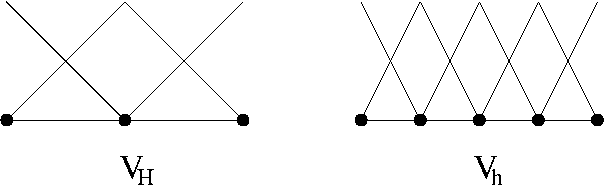
\includegraphics[height=2cm]{pictures/prol}
\end{center}
The first basis function $\varphi_1^H$ is
$$
\varphi_1^H = \varphi_1^h + \frac{1}{2} \varphi_2^h
$$
The whole matrix is
$$
E_H = 
\left( \begin{array}{ccc}
        1 \\
        1/2 & 1/2 \\
         & 1 & \\
        & 1/2 & 1/2 \\
        & & 1 
        \end{array} \right).
$$

There holds
$$
G_H \ul u_H = G_h E_H \ul u_H.
$$
Proof:
\begin{eqnarray*}
G_H \ul u_H & = & \sum_{i=1}^{N_H} u_{H,i} \varphi_i^H = \sum_{i=1}^{N_H} \sum_{j=1}^{N_h} u_{H,i} E_{H,ji} \varphi_j^h \\
        & = & \sum_{j=1}^{N_h} \varphi_j^h (E_H \ul u_H)_j = G E \ul u_H
\end{eqnarray*}
The matrix $E_H$ transforms the coefficients $\ul u_H$ w.r.t. the
coarse grid basis to the coefficients $\ul u_h = E_H \ul u_H$ w.r.t. the
fine grid basis. It is called {\em prolongation matrix}.

\medskip

The DD preconditioner with coarse grid correction is
$$
C^{-1} \times d = \sum_i E_i A_i^{-1} E_i^T d + E_H (E_H^T A E_H)^{-1} E_H^T d 
$$

The first part is the local DD preconditioner from above. The second part is
the coarse grid correction step. The matrix $E_H^T$ (called {\em restriction matrix}) transfers the defect $d$ from the fine grid to a defect vector on 
the coarse grid. Then, the coarse grid problem with matrix $E_H^T A E_H$
is solved. Finally, the result is prolongated to the fine grid. 

The matrix $A_H := E_H^T A E_H$ is the Galerkin matrix w.r.t. the coarse grid
basis:
\begin{eqnarray*}
A_{H,ij} & = & \ul e_j^T E_H^T A E_H \ul e_i = A(G_h E_H \ul e_i, G_h E_H \ul e_j) \\
        & = & A(G_H \ul e_i, G_H \ul e_j) = A(\varphi_i^H, \varphi_j^H).
\end{eqnarray*}

\begin{theorem} The overlapping domain decomposition preconditioner with
coarse grid system fulfills the optimal spectral estimates
$$
\ul u^T C \ul u \leqc \ul u^T A \ul u \leqc \ul u^T C \ul u.
$$
\end{theorem}
{\em Proof:} The quadratic form generated by the preconditioner is
$$
\ul u^T C \ul u = \inf_{u_H \in V_H, u_i \in V_i  \atop u = u_H + \sum u_i}
\| u_H \|_A^2 + \sum_{i=1}^M \| u_i \|_A^2.
$$
Again, the upper bound $\ul u^T A \ul u \leqc \ul u^T C \ul u$ follows from
the finite overlap of the spaces $V_H, V_1, \ldots V_M$. To prove the lower
bound, we come up with an explicit decomposition. We split the minimization 
into two parts:
\begin{equation}
\label{equ_ddc1}
\ul u^T C \ul u = \inf_{u_H \in V_H} \inf_{u_i \in V_i  \atop u-u_H = \sum u_i}
\| u_H \|_A^2 + \sum_{i=1}^M \| u_i \|_A^2
\end{equation}
In the analysis of the DD precondition without coarse grid system we have
observed that
$$
\inf_{u_i \in V_i  \atop u-u_H = \sum u_i} \sum_{i=1}^M \| u_i \|_A^2 \leqc
H^{-2} \| u - u_H \|_{L_2}^2 + \| \nabla (u-u_H) \|_{L_2}^2
$$
Using this in (\ref{equ_ddc1}) gives
\begin{eqnarray*}
\ul u^T C \ul u & \leqc & \inf_{u_H \in V_H}  \left\{ \| u_H \|_A^2 + H^{-2} \, \| u - u_H \|_{L_2}^2 + \| \nabla (u - u_H) \|_{L_2}^2 \right\} \\
        & \leqc & \inf_{u_H \in V_H} \left\{ \| \nabla u_H \|_{L_2}^2 + H^{-2} \, \| u - u_H \|_{L_2}^2 + \| \nabla u \|_{L_2}^2 \right\}
\end{eqnarray*}

To continue, we introduce a Cl\'ement operator $\Pi_H : H^1 \rightarrow V_H$
being continuous in the $H^1$-semi-norm, and approximating in $L_2$-norm:
$$
\| \nabla \Pi_H u \|_{L_2}^2 + H^{-2} \| u - \Pi_H u \|_{L_2}^2 \leqc \| \nabla u \|_{L_2}^2
$$
Choosing now $u_H := \Pi_H u$ in the minimization problem we obtain the result:
\begin{eqnarray*}
\ul u^T C \ul u & \leqc & \| \nabla \Pi_H u \|_A^2 + H^{-2} \, \| u - \Pi_H u \|_{L_2}^2 + \| \nabla u \|_{L_2}^2 \\
        & \leqc & \| \nabla u \|^2 \eqc \| u \|_A^2
\end{eqnarray*}
\hfill $\Box$

The inverse factor $H^{-2}$ we have to pay for the local decomposition could 
be compensated by the approximation on the coarse grid. 

\bigskip
The costs for the setup depend on the underlying direct solver for the coarse
grid problem and the local problems. Let the factorization step have time
complexity $N^\alpha$. Let $N$ be the number of unknowns at the fine grid,
and $M$ the number of sub-domains. Then the costs to factor the coarse grid
problem and the $M$ local problems are  of order
$$
M^\alpha + M \left( \frac{N}{M} \right)^\alpha
$$
Equilibrating both terms gives the optimal choice of number of sub-domains
$$
M = N^\frac{\alpha}{2 \alpha-1},
$$
and the asymptotic costs
$$
N^\frac{\alpha^2}{2 \alpha-1}.
$$
Example: A Cholesky factorization using bandwidth optimization for 2D problems
has time complexity $N^2$. The optimal choice is $M = N^{2/3}$, leading to
the costs of 
$$
N^{4/3}.
$$

\bigskip

\subsubsection{Multi-level preconditioners}
The preconditioner above uses two grids, the fine one where the equations
are solved, and an artificial coarse grid. Instead of two grids, one
can use a whole hierarchy of grids ${\cal T}_0, {\cal T}_1, \ldots , {\cal T_L} = {\cal T}$. The according finite element spaces are
$$
V_0 \subset V_1 \subset \ldots \subset V_L = V_h.
$$
Let $E_l$ be the prolongation matrix from level $l$ to the finest level $L$.
Define
$$
A_l = E_l^T A E_l \qquad \mbox{and} \qquad D_l = \mbox{diag} \{ A_l \}.
$$
Then, the multi-level preconditioner is
$$
C^{-1} = E_0 A_0^{-1} E_0^T + \sum_{l=1}^L E_l D_l^{-1} E_l^T
$$

The setup, and the application of the preconditioner takes
$O(N)$ operations. One can show that the multi-level preconditioner
fulfills optimal spectral bounds
$$
\ul u^T  C \ul u \leqc \ul u^T A \ul u \leqc \ul u^T C \ul u.
$$

An iterative method with multi-level preconditioning solves the
matrix equation $A u = f$ of size $N$ with $O(N)$ operations !


% \documentclass[12pt]{article}
% \usepackage{amsmath,amsthm,amssymb,a4wide}
% \usepackage[german,english]{babel}
% \usepackage{epsfig}
% \usepackage{latexsym}
% \usepackage{amssymb}
% % \usepackage{theorem}
% \usepackage{amsthm}
% % \usepackage{showkeys}

% \newcommand{\setR}{ {\mathbb R} }
% \newcommand{\setN}{ {\mathbb N} }
% \newcommand{\setZ}{ {\mathbb Z} }
% \newcommand{\eps}{\varepsilon}

% \newcommand{\beq}{\begin{equation}}
% \newcommand{\eeq}{\end{equation}}

% \newcommand{\opdiv}{\operatorname{div}}
% \newcommand{\opcurl}{\operatorname{curl}}
% \newcommand{\opdet}{\operatorname{det}}
% \newcommand{\optr}{\operatorname{tr}}
% \newcommand{\optrn}{\operatorname{tr}_n}
% \newcommand{\sfrac}[2]{ { \textstyle \frac{#1}{#2} } }

% \newcommand{\Zh}{\mathrm{Z}_h}
% \newcommand{\Ih}{\mathrm{I}_l}

% \newcommand{\leqc}{\preceq} 
% \newcommand{\geqc}{\succeq} 
% \newcommand{\eqc}{\simeq} 
% \newcommand{\ul}{\underline}

% \newtheorem{theorem}{Theorem}
% \newtheorem{definition}[theorem]{Definition}
% \newtheorem{lemma}[theorem]{Lemma}
% \newtheorem{remark}[theorem]{Remark}
% \newtheorem{example}[theorem]{Example}

% %
% %
% \setlength{\unitlength}{1cm}
% \sloppy 
% %

% \title{Analysis of the multi-level preconditioner}
% \author{Joachim Sch\"oberl}

% \begin{document}
% \maketitle

\section{Analysis of the multi-level preconditioner}

We want to solve a finite element system on $V_L := V_h \subset H^1$.
To define the multi-level preconditioner $C = C_L$, we use also finite
element spaces on coarser meshes ${\mathcal T}_0, {\mathcal T}_1, \ldots
{\mathcal T}_L$:
$$
V_0 \subset V_1 \subset \ldots \subset V_L
$$
Assume $h_l \eqc 2^{-l}$. Let $\{ \varphi_{l,i} : 1 \leq i \leq N_l \}$ be the hat-basis for $V_l$, with $N_l = \operatorname{dim} V_l$. 
Let $A_l$ be the finite element matrix on $V_l$.

$E_l \in \setR^{N_l \times N_{l-1}}$ is the prolongation matrix from level~$l-1$ to level~$l$.

The multi-level preconditioner is defined recursively:
\begin{eqnarray*}
C_0^{-1} & := & A_0^{-1} \\
C_l^{-1} & := & (\operatorname{diag}A_l)^{-1} + E_l C_{l-1}^{-1} E_l^T \quad 1 \leq l \leq L.
\end{eqnarray*}
The computational complexity of one application of $C_L^{-1}$ is $O(N)$ operations.

(An extended version of) the Additive Schwarz Lemma allows to 
rewrite 
\begin{eqnarray*}
\| u_l \|_{C_l}^2 & = &
\inf_{u_l = u_{l-1} + \sum_{i=1}^{N_l} u_{l,i} \atop
  u_{l-1} \in V_{l-1}, u_{l,i} \in \operatorname{span} \{\varphi_{l,i}} \}
  \| u_{l-1} \|_{C_{l-1}}^2 + \sum_{i=1}^{N_l} \| u_{l,i} \|_A^2 \\ 
 & = & \inf_{u = u_0 + \sum_{l=1}^L \sum_{i=1}^{N_l} u_{l,i}}
 \sum_l \sum_i \| u_{l,i} \|_A^2 + \| u_0 \|_A^2
\end{eqnarray*}

Reordering the minimization we obtain
\begin{eqnarray*}
\| u \|_{C_L}^2 & = & \inf_{u = \sum_{l=0}^L u_l \atop u_l \in V_l}
\| u_0 \|_A^2 + \sum_{l=1}^L \inf_{u_l = \sum u_{l,i}} \sum_{i=1}^{N_l} \| u_{l,i} \|_A^2 \\
& \eqc & \inf_{u = \sum_{l=0}^L u_l \atop u_l \in V_l}
\| u_0 \|_A^2 + \sum_{l=1}^L h_l^{-2} \| u_l \|_{L_2}^2
\end{eqnarray*}

\begin{lemma} [simple analysis] 
$$
\frac{1}{L} C \leqc  A \leqc L C
$$
\end{lemma}
\begin{proof} $A \leqc L C$ follows from maximal overlap of spaces and
the inverse estimate $\| \nabla u_l \|_{L_2} \leqc h_l^{-1} \| u_l \|_{L_2}$. Let $u = \sum_{l=0}^L u_l$ be an arbitrary decomposition:
$$
\| \sum_{l=0}^L u_l \|_A^2 \leq (L+1) \sum_{l=0}^L \| u_l \|_A^2 
\leqc L  \big( \| u_0 \|_A^2 + \sum_{l=1}^L h_l^{-2} \| u_l \|_{L_2}^2 \big).
$$
Since the estimate holds for any decompositon, it also holds for the infimum.
\medskip

To show $C \leqc L A$ we come up with an explicit decomposition of $u \in V_L$. Let $\Pi_l : L_2 \rightarrow V_l$ be a Cl\'ement-type operator which is a projection and satisfies
$$
\| \Pi_l u \|_{H^1} + h_l^{-1} \, \| u - \Pi_l u \|_{L_2} \leqc \| u \|_{H^1} \qquad \forall \, u \in H^1.
$$
Define 
\begin{eqnarray*}
u_0 & := & \Pi_0 u \\
u_l & := & \Pi_l u - \Pi_{l-1} u \qquad 1 \leq l \leq L.
\end{eqnarray*}
Then $u = \sum_{l=0}^L u_l$ and
$$
\| u \|_C^2 \leqc \| \Pi_0 u \|_A^2 + \sum_{l=1}^L h_l^{-2} \| \Pi_l u  - \Pi_{l-1} u \|_{L_2}^2 \leqc L  \, \| u \|_{H^1}^2 \approx \| u \|_A^2
$$
We have bound each of the $L+1$ terms by the $H^1$-norm of $u$, thus the factor $L$.
\end{proof}

Next we show an improved estimate leading to the optimal condition number $\kappa (C^{-1} A) \leqc 1$, independent of the number of refinement levels:
\begin{lemma} There holds
$$
C \leqc A \leqc C
$$
\end{lemma}
\begin{proof} We show $A \leqc C$. Let $u = \sum_{l=0}^L u_l$ an 
arbitrary decomposition. First, we split up the coarsest level:
$$
\| u \|_A^2 \leq \| u_0 \|_A^2 + \| \sum_{l=1}^L u_l \|_A^2
$$
Next we show the estimate
$$
A(u_l, v_k) \leq 2^{-\frac{|l-k|}{2}} h_l^{-1} \| u_l \| h_k^{-1} \| v_k \|
\qquad \forall \, u_l \in V_l, \; v_k \in V_k
$$
We assume $l \leq k$. We perform integration by parts on the level-l triangles, and apply Cauchy-Schwarz and scaling techniques:
\begin{eqnarray*}
A(u_l, v_k) & = & \sum_{T \in {\mathcal T}_l} \int_T \nabla u_l \nabla v_k \\
& \leq & \sum_T  \int_T \underbrace{-\Delta u_l}_{= 0} v_k + \int_{\partial T} \frac{\partial u_l}{\partial n} v_k \\
& \leq & \sum_T \left\| \frac{\partial u_l}{\partial n} \right\|_{\partial T_l} \, \| v_k \|_{\partial T_l} \\
& \leq & h_l^{-3/2} \| u_l \|_{L_2} \, h_k^{-1/2} \| v_k \|_{L_2} \\
& = & \underbrace{\sqrt{h_k/h_l}}_{\eqc 2^{-|k-l|/2}} \, h_l^{-1} \| u_l \|_{L_2} \, h_k^{-1} \| v_k \|_{L_2}
\end{eqnarray*}
We define the overlap - matrix ${\mathcal O} \in \setR^{L \times L}$ as
$$
{\mathcal O}_{kl} = 2^{-|k-l|/2}.
$$
Then
\begin{eqnarray*}
\| \sum_{l=1}^L u_l \|_A^2 & = & 
\sum_{l,k=1}^N A(u_l, u_k) \leqc \sum_{l,k} {\mathcal O}_{kl} h_k^{-1} \| u_k \|_{L_2} \, h_l^{-1} \| u_l \|_{L_2} \\
& \leq & \rho (\mathcal O) \, \sum_{l=1}^L h_l^{-2} \| u_l \|^2_{L_2}
\end{eqnarray*}
The spectral radius $\rho ({\mathcal O})$ can be estimated by the row-sum-norm, which is bounded by a convergent geometric sequence
$$
\sum_{k=1}^L 2^{-|k-l|/2} \leq 2 \sum_{k=0}^\infty \sqrt{2}^{-k} 
\leq \frac{2}{1-\sqrt{2}}.
$$
Since the decomposition was arbitrary, the estimate holds for the minimal decomposition.


\bigskip

Now we show $C \leqc A$. We procede similar as above. 
Let $\Pi_l : L_2 \rightarrow V_l$ be an Cl\'ement-type operator 
such that
\begin{eqnarray*}
\| \Pi_l u \|_{L_2} & \leq & \| u \|_{L_2}  \qquad \forall \, u \in L_2 \\
\| u - \Pi_l u \|_{L_2} & \leqc & h_l^2 \| u \|_{H^2} \quad \forall \, u \in H^2.
\end{eqnarray*}
We define $u_0 = \Pi_0 u$ and $u_l = \Pi_l u - \Pi_{l-1} u$. We obtain
the 2 estimates
\begin{eqnarray*}
h_l^{-2} \| u_l \|_{L_2}^2 & \leqc & h_l^{-2} \| u \|_{L_2}^2, \\
h_l^{-2} \| u_l \|_{L_2}^2 & \leqc & h_l^2 \| u \|_{H^2}.
\end{eqnarray*}
The idea of the proof is that $H^1$ is the interpolation space $[L_2, H^2]_{1/2}$. We define the K-functional
$$
K(t,u)^2 = \inf_{u = u_0 + u_2 \atop u_0 \in L_2, u_2 \in H^2}
\big\{ \| u_0 \|_{L_2}^2 + t^2 \| u_2 \|_{H^2}^2 \big\}.
$$
Combining the 2 estimates above we get
$$
h_l^{-2} \| u_l \|_{L_2}^2 \leqc h_l^{-2} K^2 (h_l^2, u)
$$
Thus, the sum over $L$ levels is
$$
\sum_{l=1}^L h_l^{-2} \| u_l \|_{L_2}^2 \leq \sum_{l=1}^L h_l^{-2} K^2 (h_l^2, u) \eqc \sum_{l=1}^L 2^l K^2(2^{-l}, u)
$$
Next we use that $K(s,.) \eqc K(t,.)$ for $t \leq s \leq 2t$ and replace
the sum by an integral, and substitute $t := 2^{-l}, dt \eqc -2^{-l} dl = t dl$:
\begin{eqnarray*}
\sum_{l=1}^L h_l^{-2} \| u_l \|_{L_2}^2 & \leq & 
\int_{l=1}^{L+1} 2^l K^2(2^{-l}, u) dl \\
& \eqc & \int_{2^{-L-1}}^1 t^{-1} K^2(t,u) \frac{dt}{t}  \\
& \leqc & \int_0^\infty t^{-1} K^2(t,u) \frac{dt}{t} \\
& = & \| u \|_{[L_2,H^2]_{1/2}} \eqc \| u \|_{H^1}
\end{eqnarray*}
\end{proof}
An intuitive explanation of the proof is that different terms of 
the sum
$\sum_{l=1}^L h_l^{-2} \| \Pi_l u - \Pi_{l-1} u \|_{L_2}$ 
are dominated by different frequency 
components of $u$. The squared $H^1$-norm is the sum over $H^1$-norms of
the individual frequency components.

% \end{document}

\chapter{Mixed Methods}

A mixed method is a variational formulation involving two function spaces, 
and a bilinear-form of a special saddle point structure. Usually, it is
obtained from variational problems {\em with constraints}.

\section{Weak formulation of Dirichlet boundary conditions}

We start with the Poisson problem
\begin{equation} \label{equ_mixeddirpde}
-\Delta u = f \qquad \mbox{in} \; \Omega,
\end{equation}
and boundary conditions
$$
\begin{array}{rcll}
u & = & u_D \qquad & \mbox{on} \; \Gamma_D, \\
\frac{\partial u}{\partial n} & = & 0 & \mbox{on} \; \Gamma_N.
\end{array}
$$
In contrast to the earlier method, we multiply equation (\ref{equ_mixeddirpde})
with test functions $v \in H^1$ (without imposing Dirichlet constraints), 
and integrate by parts. Using the Neumann boundary conditions, we obtain
$$
\int_\Omega \nabla u \nabla v \, dx - \int_{\Gamma_D} \frac{\partial u}{\partial n} \, v \, ds = \int_\Omega f v \, dx
$$
The normal derivative $\frac{\partial u}{\partial n}$ is not known on $\Gamma_D$. We simply call it $-\lambda$:
$$
\lambda := - \frac{\partial u }{\partial n}
$$
To pose the Dirichlet boundary condition, we multiply $u = u_D$ by sufficiently many test functions, and integrate over $\Gamma_D$:
$$
\int_{\Gamma_D} u \mu \, ds = \int_{\Gamma_D} u_D \mu \, ds \qquad \forall \, 
\mu \in \; ?
$$

Combining both equations, we get the system of equations:
Find $u \in V = H^1(\Omega)$ and $\lambda \in Q = ?$ such
that
\begin{equation} \label{equ_mixeddirichlet}
\begin{array}{ccccll}
\int_\Omega \nabla u \cdot \nabla v \, dx & + & \int_{\Gamma_D} v \lambda \, ds & = & \int f v \, dx \quad & \forall \, v \in V, \\[0.5em]
\int_{\Gamma_D} u \mu \, ds & & & = & \int_{\Gamma_D} u_D \mu \, ds \quad & \forall \, \mu \in Q.
\end{array}
\end{equation}
A similar formulation can be obtained for interface conditions.

\section{A Mixed method for the flux}

We start from the second order pde
$$
\opdiv (a \nabla u) = f \qquad \mbox{in} \; \Omega,
$$
and boundary conditions
\begin{eqnarray*}
u & = & u_D \qquad \mbox{on} \, \Gamma_D \\
a \frac{\partial u}{\partial n} & = & g \qquad \mbox{on} \, \Gamma_N
\end{eqnarray*}
Next, we introduce the flux variable $\sigma := a \nabla u$
to rewrite the equations as: Find $u$ and $\sigma$ such that
\begin{eqnarray}
a^{-1} \sigma - \nabla u & = & 0,   \label{equ_mixedsigma}  \\
\opdiv \, \sigma & = & -f,       \label{equ_mixedu}
\end{eqnarray}
and boundary conditions
\begin{eqnarray*}
u & = & u_D \qquad \mbox{on} \, \Gamma_D \\
\sigma \cdot n & = & g \qquad \mbox{on} \, \Gamma_N.
\end{eqnarray*}

We want to derive a variational formulation for the system of equations.
For that, we multiply the first equations by vector-valued test functions~$\tau$, the second equation by test functions $v$, and integrate:
$$
\begin{array}{ccccll}
\int_\Omega (a^{-1} \sigma) \cdot \tau \, dx & - & \int_\Omega \tau \cdot \nabla u \, dx & = & 0 \qquad & \forall \, \tau \\[0.5em]
\int_\Omega \opdiv \, \sigma \, v \, dx & & & = & - \int f v \, dx \qquad & \forall \, v
\end{array}
$$
We would like to have the second term of the first equation of the same
structure as the first term in the second equation. This can be obtained
by integration by parts applied to either one of them. The interesting
case is to integrate by parts in the first line to obtain:
$$
\int_\Omega (a^{-1} \sigma) \cdot \tau \, dx + \int_\Omega \opdiv \, \tau \, u \, dx
-\int_{\Gamma_D} \tau_n \, u \, ds - \int_{\Gamma_N} \tau_n \, u \, ds = 0.
$$
Here, we make use of the boundary conditions. On the Dirichlet boundary,
we know $u = u_D$, and use that in the equation. The Neumann boundary
condition $\sigma \cdot n = g$ must be put into the approximation space,
it becomes an essential boundary condition. Thus, it is enough to choose
test functions of the sub-space fulfilling $\tau \cdot n = 0$.
The problem is now the following. The space $V$ will be fixed later.
Find $\sigma \in V, \sigma_n = g$ on $\Gamma_N$, and $u \in Q$
such that
$$
\begin{array}{ccccll}
\int_\Omega (a^{-1} \sigma) \cdot \tau \, dx & + & 
\int_\Omega \opdiv \, \tau  \, u \, dx & = & \int_{\Gamma_D} u_D \tau _n \, ds \qquad & \forall \, \tau, \; \tau_n = 0 \; \mbox{on} \; \Gamma_N \\
\int_\Omega \opdiv \, \sigma \, v \, dx & & & = & - \int f v \, dx \qquad & \forall \, v
\end{array}
$$
The derivatives are put onto the flux unknown $\sigma$ (and its test function $\tau$).
We don't have to derive the primal unknown $u$. This will give us better
approximation for the fluxes than for the scalar. That is one of the reasons
to use this mixed method.


\section{Abstract theory}

A mixed variational formulation involves two Hilbert spaces $V$ and $Q$,
bilinear-forms
\begin{eqnarray*}
a(u,v) & : & V \times V  \rightarrow \setR, \\
b(u,q) & : & V \times Q  \rightarrow \setR,
\end{eqnarray*}
and continuous linear-forms
\begin{eqnarray*}
f(v) & : & V \rightarrow \setR, \\
g(q) & : & Q \rightarrow \setR.
\end{eqnarray*}
%
The problem is to find $u \in V$ and $p \in Q$ such that
\begin{equation}
\begin{array}{ccccll}
a(u,v) & + & b(v,p) & = & f(v) \quad & \forall \, v \in V, \\[0.2em]
b(u,q) & & & = & g(q) \quad & \forall \, q \in Q.
\end{array}
\end{equation}
%
The two examples from above are of this form.


\bigskip

Instead of considering this as a system of equations, one can look at
the mixed method as one variational problem on the product spaces $V \times Q$.
For this, simply add both lines, and search for $(u,p) \in V \times Q$ such that
$$
a(u,v) + b(u,q) + b(v,p) = f(v) + g(q) \qquad \forall \, (v,q) \in V \times Q.
$$
Define the big bilinear-form $B(.,.) : (V \times Q) \times (V \times Q) \rightarrow \setR$ as
$$
B( (u,p), (v,q) ) = a(u,v) + b(u,q) + b(v,p),
$$
to write the whole system as single variational problem
$$
\mbox{Find } (u,p) \in V \times Q : \qquad
B((u,p),(v,q)) = f(v) + g(q) \qquad \forall \, (v,q) \in V \times Q
$$

\bigskip

By the Riesz-representation theorem, we can define operators:
$$
\begin{array}{lllrcl}
A : & V \rightarrow V : & u \rightarrow A u : & (Au,v)_V & = & a(u,v) \quad \forall \, v \in V \\
B : & V \rightarrow Q : & u \rightarrow B u : & (Bu,q)_Q & = & b(u,q) \quad \forall \, q \in Q \\
B^* : & Q \rightarrow V : & p \rightarrow B^* p : & (B^*p,v)_V & = & b(v,p) \quad \forall \, v \in V.
\end{array}
$$
By means of these operators, we can write the mixed variational problem as
operator equation
\begin{equation}
\begin{array}{ccccl}
A u & + & B^* p & = J_V f, \\
B u & & & = J_Q g.
\end{array}
\end{equation}
Here, we used the Riesz-isomorphisms $J_V : V^\ast \rightarrow V$ and $J_Q : Q^\ast \rightarrow Q$. 

\bigskip

In the interesting examples, the operator $B$ has a large kernel:
$$
V_0 := \{ v : B v = 0 \}
$$
\begin{lemma} Assume that $B^\ast Q$ is closed in $V$. Then there holds 
the $V$-orthogonal decomposition
$$
V = V_0 + B^\ast Q
$$
\end{lemma}
{\em Proof:} There holds
\begin{eqnarray*}
V_0 & = & \{ v : B v = 0 \} \\
   & = & \{ v : (B v, q)_Q = 0  \quad \forall \, q \in Q\} \\
   & = & \{ v : (v, B^\ast q)_V = 0 \quad \forall \, q \in Q \}.
\end{eqnarray*}
This means, $V_0$ is the $V$-orthogonal complement to $B^\ast Q$.
\hfill $\Box$


Now, we will give conditions to ensure a unique solution of a mixed
problem:
\begin{theorem}[Brezzi's theorem] \label{theo_brezzi}
Assume that $a(.,.)$ and $b(.,.)$ are continuous bilinear-forms
\begin{eqnarray}
a(u,v) & \leq & \alpha_2 \, \| u \|_V \,  \| v \|_V \qquad \forall \, u,v \in V, \\
b(u,q) & \leq & \beta_2 \, \| u \|_V \, \| q \|_Q \qquad \forall \, u \in V, \; 
\forall \, q \in Q.
\end{eqnarray}
Assume there holds coercivity of $a(.,.)$ on the kernel,i.e.,
\begin{equation} \label{equ_kernelell}
a(u,u) \geq \alpha_1 \, \| u \|_V^2 \qquad \forall \, u \in V_0,
\end{equation}
and there holds the LBB (Ladyshenskaja-Babu\v{s}ka-Brezzi) condition
\begin{equation} \label{equ_lbb}
\sup_{u \in V} \frac{b(u,q)}{\|u\|_V} \geq \beta_1 \, \| q \|_Q \quad \forall \, q \in Q.
\end{equation}
Then, the mixed problem is uniquely solvable. The solution fulfills
the stability estimate
$$
\| u \|_V + \| p \|_Q \leq c \{ \| f \|_{V^\ast} + \| g \|_{Q^\ast} \},
$$
with the constant $c$ depending on $\alpha_1, \alpha_2, \beta_1, \beta_2$.
\end{theorem}
{\em Proof:} The big bilinear-form $B(.,.)$ is continuous
$$
B((u,p),(v,q)) \leqc ( \| u \| + \| p \| ) \, ( \| v \| + \| q \| ).
$$
We prove that it fulfills the $\inf-\sup$ condition
$$
\inf_{v,q} \sup_{u,p} \frac{B((u,p),(v,q))}{ ( \|v\|_V+\|q\|_Q) (\|u\|_V+\|p\|_Q)} \geq \beta.
$$
Then, we use Theorem~\ref{theo_infsup} (by Babu\v{s}ka-Aziz) to conclude
continuous solvability.

To prove the $\inf-\sup$-condition, we choose 
arbitrary $v \in V$ and $q \in Q$. We will construct $u \in V$ and 
$p \in Q$ such that
$$
\| u \|_V + \| p \|_Q \leqc \| v \|_V + \| q \|_Q
$$
and
$$
B((u,p),(v,q)) = \| v \|_V^2 + \| q \|_Q^2.
$$
First, we use (\ref{equ_lbb}) to choose $u_1 \in V$ such that
$$
b(u_1,q) = \| q \|_Q^2 \qquad \mbox{and} \qquad \| u_1 \|_V \leq 2 \beta_1^{-1} \, \| q \|_Q.
$$
Next, we solve a problem on the kernel:
$$
\mbox{Find } u_0 \in V_0 : \quad
a(u_0, w_0) = (v,w_0)_V - a(u_1, w_0) \qquad \forall \, w_0 \in V_0
$$
Due to assumption (\ref{equ_kernelell}), the left hand side is a coercive 
bilinear-form on $V_0$. The right hand side is a continuous linear-form.
By Lax-Milgram, the problem has a unique solution fulfilling
$$
\| u_0 \|_V \leqc \| v \|_V + \| u_1 \|_V
$$
We set 
$$
u = u_0 + u_1.
$$
By the Riesz-isomorphism, we define a $z \in V$ such that
$$
(z,w)_V = (v,w)_V - a(u, w) \qquad \forall \, w \in V
$$
By construction, it fulfills $z \bot_V V_0$. The LBB condition implies
$$
\| p \|_Q \leq 
\beta_1^{-1} \sup_v \frac{b(v,p)}{\| v\|_V} 
= \beta_1^{-1} \sup_v \frac{(v, B^\ast p)_V}{\| v\|_V} 
= \beta_1^{-1} \| B^\ast p \|_V,
$$
and thus $B^\ast Q$ is closed, and $z \in B^\ast Q$. Take the $p \in Q$ such that
$$
z = B^\ast p.
$$
It fulfills
$$
\| p \|_Q \leq \beta_1^{-1} \| z \|_V \leqc \| v \|_V + \| q \|_Q
$$
Concluding, we have constructed $u$ and $p$ such that
$$
\| u \|_V + \| p \|_Q \leqc \| v \|_V + \| q \|_Q,
$$
and
\begin{eqnarray*}
B((u,p),(v,q)) & = & a(u,v) + b(v,p) + b(u,q) \\
        & = & a(u,v) + (z,v)_V + b(u,q) \\
        & = & a(u,v) + (v,v)_V - a(u,v) + b(u,q) \\
        & = & \| v \|_V^2 + b(u_1, q) \\
        & = & \| v \|_V^2 + \| q \|_Q^2.
\end{eqnarray*}
\hfill $\Box$

\section{Analysis of the model problems}
Now, we apply the abstract framework to the two model problems.

\subsubsection{Weak formulation of Dirichlet boundary conditions}

The problem is well posed for the spaces
$$
V = H^1(\Omega) \qquad \mbox{and} \qquad Q = H^{-1/2}(\Gamma_D)
$$
Remember, $H^{-1/2}(\Gamma_D)$ is the dual to $H^{1/2}(\Gamma_D)$.
The later one is the trace space of $H^1(\Omega)$, the norm fulfills
$$
\| u_D \|_{H^{1/2}(\Gamma_D)} \eqc \inf_{ w \in H^1 \atop \optr \, w = u_D} \| w \|_{H^1(\Omega)}.
$$
The bilinear-forms are
\begin{eqnarray*}
a(u,v) & = & \int_\Omega \nabla u \, \nabla v \, dx  \\
b(u,\lambda) & = & \left< \lambda, \optr \, u \right>_{H^{-1/2} \times H^{1/2}}
\end{eqnarray*}
To be precise, the integral $\int_{\Gamma_D} \lambda u \, dx$ is extended
to the duality product $\left< \lambda, u \right>$. For regular 
functions ($\lambda \in L_2(\Gamma_D)$), we can write the $L_2$-inner
product.

\begin{theorem} The mixed problem (\ref{equ_mixeddirichlet}) has
a unique solution $u \in H^1(\Omega)$ and $\lambda \in H^{-1/2}(\Gamma_D)$.
\end{theorem}
{\em Proof:} 
The spaces $V$ and $Q$, and the bilinear-forms $a(.,.)$ and
$b(.,.)$ fulfill the assumptions of Theorem~\ref{theo_brezzi}.
The kernel space $V_0$ is
$$
V_0 = \{ u : \int_{\Gamma_D} u \mu \, dx = 0 \; \quad \forall \, \mu \in L_2(\Gamma_D) \} = \{ u : \optr_{\Gamma_D} u = 0 \}
$$
The continuity of $a(.,.)$ on $V$ is clear. It is not coercive
on $V$, but, due to Friedrichs inequality, it is coercive on $V_0$.

The bilinear-form $b(.,.)$ is continuous on $V \times Q$:
$$
b(u,\mu) = \left< \mu, \optr \, u  \right>_{H^{-1/2} \times H^{1/2} }
 \leq \| \mu \|_{H^{-1/2}} \| \optr \, u \|_{H^{1/2}(\Gamma_D)} 
 \leqc \| \mu \|_Q \| u \|_{H^1} = \| \mu \|_Q \| u \|_V
$$
The LBB - condition of $b(.,.)$ follows more or less from the definition
of norms:
\begin{eqnarray*}
\| q \|_Q & = & \sup_{u \in H^{1/2}} \frac{ \left< q, u \right> }{ \| u \|_{H^{1/2}}} \\
        & \eqc & \sup_{u \in H^{1/2}} \frac{ \left< q, u \right> }{ \inf_{w \in H^1(\Omega) \atop \optr \, w = u} \| w \|_{H^1(\Omega)}} \\
        & = & \sup_{u \in H^{1/2}} \sup_{w \in H^1(\Omega) \atop \optr \, w = u} \frac{ \left< q, u \right> }{ \| w \|_{H^1}} \\
        & = & \sup_{w \in H^1} \frac{ \left< q, \optr \, w \right> }{ \| w \|_{H^1}} 
        = \sup_{w \in V} \frac{b(w,q)}{\| w \|_V}
\end{eqnarray*}


\subsubsection{Mixed method for the fluxes}

This mixed method requires the function space $H(\opdiv, \Omega)$:

\begin{definition} A measurable function $g$ is called the weak divergence
of $\sigma$ on $\Omega \subset \setR^d$ if there holds
$$
\int_\Omega g \, \varphi \, dx = -\int_\Omega \sigma \cdot \nabla \varphi \, dx 
\qquad \forall \, \varphi \in C_0^\infty (\Omega)
$$
The function space $H(\opdiv)$ is defined as
$$
H(\opdiv,\Omega) := \{ \sigma \in [L_2(\Omega)]^d : \opdiv \, \sigma \in L_2 \},
$$
its norms is
$$
\| \sigma \|_{H(\opdiv)} = \left\{ \| \sigma \|_{L_2}^2 + \| \opdiv \, \sigma \|_{L_2}^2 \right \}^{1/2}
$$
\end{definition}

The mixed method is formulated on the spaces
$$
V = H(\opdiv) \qquad Q = L_2
$$
The bilinear-forms are
\begin{eqnarray*}
a(\sigma, \tau) & = & \int a^{-1} \sigma \tau \, dx \qquad \forall \, \sigma, \tau \in V \\
b(\sigma, v) & = & \int \opdiv \, \sigma \, v \, dx \qquad \forall \, \sigma \in V, \; \forall \, v \in Q
\end{eqnarray*}
We assume that the symmetric matrix $a \in \setR^{d\times d}$
and its inverse $a^{-1}$ are bounded.

\begin{theorem} The mixed problem for the fluxes is well posed.
\end{theorem}
{\em Proof:} We check the conditions of the theorem of Brezzi:
The bilinear-forms are bounded, namely
$$
a(\sigma, \tau) = \int a^{-1} \sigma \tau \, dx \leq \| a^{-1} \|_{L_\infty} \| \sigma \|_{L_2} \, \| \tau \|_{L_2} \leqc \| \sigma \|_V \, \| \tau \|_V
$$
and 
$$
b(\sigma, v) = \int \opdiv \, \sigma v \, dx \leq \| \opdiv \sigma \|_{L_2} \, \| v \|_{L_2} \leq \| \sigma \|_V \, \| v \|_Q.
$$

The kernel space $V_0 = \{ \tau : b(\tau, v) = 0 \; \forall \, v \in Q \}$
is
$$
V_0 = \{ \tau \in H(\opdiv) : \opdiv \, \tau = 0 \}
$$
There holds the kernel-ellipticity of $a(.,.)$. Let $\tau \in V_0$. Then
$$
a(\tau, \tau) = \int \tau^T a^{-1} \tau \, dx \geq \inf_{x\in \Omega} \lambda_{\min} (a^{-1}) \int |\tau|^2 \,dx \geqc \| \tau \|_{L_2}^2 = \| \tau \|_{H(\opdiv)}^2
$$

We are left to verify the LBB condition
\begin{equation} \label{equ_lbbhdiv}
\sup_{\sigma \in H(\opdiv)} \frac{\int \opdiv \, \sigma \,  v \, dx} { \| \sigma \|_{H(\opdiv)}}
\geqc \| v \|_{L_2} \qquad \forall \, v \in L_2.
\end{equation}
For given $v \in L_2$, we will construct a flux $\sigma$ satisfying the 
inequality.
For this, we solve the artificial Poisson problem $-\Delta \varphi = v$ with
Dirichlet boundary conditions $\varphi = 0$ on $\partial \Omega$. The solution
satisfies $\| \nabla \varphi \|_{L_2} \leqc \| v \|_{L_2}$. Set $\sigma = -\nabla \varphi$. There holds $\opdiv \, \sigma = v$. Its norm is
$$
\| \sigma \|_{H(\opdiv)}^2 = \| \sigma \|_{L_2}^2 + \| \opdiv \, \sigma \|_{L_2}^2
        = \| \nabla \varphi \|_{L_2}^2 + \| v \|_{L_2}^2 \leqc \| v \|_{L_2}^2.
$$
Using it in (\ref{equ_lbbhdiv}), we get the result
$$
\frac{ \int \opdiv \, \sigma \, v \, dx} { \| \sigma \|_{H(\opdiv)}}
 = \frac{ \int v^2 \, dx} { \| \sigma \|_{H(\opdiv)}} \geqc \| v \|_{L_2}.
$$

\subsubsection{The function space $H(\opdiv)$}

The mixed formulation has motivated the definition of the function
space $H(\opdiv)$. Now, we will study some properties of this
space. We will also construct finite elements for the approximation of
functions in $H(\opdiv)$.  In Section~\ref{sec_traceh1}, we have
investigated traces of functions in $H^1$. Now, we apply similar
techniques to the space $H(\opdiv)$. Again, the proofs are based on
the density of smooth functions.

For a function in $H^1$, the boundary values are well defined by the 
trace operator. For a vector-valued function in $H(\opdiv)$, only the 
normal-component is well defined on the boundary:

\begin{theorem} There exists a normal-trace operator 
$$
\optrn : H(\opdiv) \rightarrow H^{-1/2} (\partial \Omega)
$$
such that for $\sigma \in H(\opdiv) \cap [C(\overline \Omega)]^d$ it coincides with
its normal component
$$
\optrn \sigma = \sigma \cdot n \qquad \mbox{on} \; \partial \Omega.
$$
\end{theorem}
{\em Proof:} For smooth functions, the trace operator gives the normal
component on the boundary. We have to verify that this operator is bounded
as operator from $H(\opdiv)$ to $H^{-1/2}(\partial \Omega)$. Then, by 
density, we can extend the trace operator to $H(\opdiv)$. Let $\sigma \in H(\opdiv) \cap [C^1(\overline \Omega)]^d$:
\begin{eqnarray*}
\| \optrn \sigma \|_{H^{-1/2}} 
& = & \sup_{\varphi \in H^{1/2}(\partial \Omega)} \frac{ \int_{\partial \Omega} \sigma \cdot n \, \varphi \, ds } { \| \varphi \|_{H^{1/2} }} 
\eqc 
\sup_{\varphi \in H^1(\Omega)} \frac{ \int_{\partial \Omega} \sigma \cdot n \, \optr \, \varphi \, ds } { \| \varphi \|_{H^1 }} \\
& = & 
\sup_{\varphi \in H^1(\Omega)} \frac{ \int_{\partial \Omega} (\sigma \, \optr \, \varphi) \cdot n \, ds } { \| \varphi \|_{H^1 }} 
=
\sup_{\varphi \in H^1(\Omega)} \frac{ \int_{\Omega} \opdiv (\sigma  \varphi) \, dx } { \| \varphi \|_{H^1 }} \\
& = & 
\sup_{\varphi \in H^1(\Omega)} \frac{ \int_{\Omega} (\opdiv \sigma)  \varphi \, dx +   \int_{\Omega} \sigma \cdot \nabla \varphi \, dx } { \| \varphi \|_{H^1 }} \leq
\sup_{\varphi \in H^1(\Omega)} \frac{ \| \opdiv \sigma \|_{L_2} \, \| \varphi \|_{L_2} + \| \sigma \|_{L_2} \, \| \nabla \varphi \|_{L_2} } { \| \varphi \|_{H^1 }} \\
& \leq & \left\{ \| \sigma \|_{L_2}^2 + \| \opdiv \, \sigma \|_{L_2}^2 \right\}^{1/2}
 = \| \sigma \|_{H(\opdiv)}
\end{eqnarray*}
\hfill $\Box$

\medskip

\begin{lemma} There holds integration by parts
$$
\int_\Omega \sigma \cdot \nabla \varphi \, dx + \int_\Omega (\opdiv \, \sigma) \varphi \, dx = \left< \optrn \, \sigma , \optr \varphi \right>_{H^{-1/2} \times H^{1/2}}
$$
for all $\sigma \in H(\opdiv)$ and $\varphi \in H^1(\Omega)$.
\end{lemma}
{\em Proof:} By density of smooth functions, and continuity of the trace operators.

\medskip

Now, let $\Omega_1, \ldots \Omega_M$ be a non-overlapping partitioning of $\Omega$.
In Section~\ref{sec_traceh1}, we have proven that functions which are 
in $H^1(\Omega_i)$, and which are continuous across the boundaries 
$\gamma_{ij} = \overline \Omega_i \cap \overline \Omega_j$, are in $H^1(\Omega)$. 
A similar property holds for functions in $H(\opdiv)$. 

\begin{theorem} Let $\sigma \in [L_2(\Omega)]^d$ such that
\begin{itemize}
\item
$$
\sigma|_{\Omega_i} \in H(\opdiv, \Omega_i)
$$
\item
$$
\optr_{n,i} \sigma|_{\Omega_i} = - \optr_{n,j} \sigma|_{\Omega_j} \qquad \mbox{ on } \gamma_{ij}.
$$
\end{itemize}
Then $\sigma \in H(\opdiv, \Omega)$, and 
$$
(\opdiv \, \sigma)|_{\Omega_i} = \opdiv \, (\sigma|_{\Omega_i}).
$$
\end{theorem}
The proof follows the lines of Theorem~\ref{theo_subdomainh1}.

\bigskip

We want to compute with functions in $H(\opdiv)$. For this, we need
finite elements for this space. The characterization by sub-domains
allows the definition of finite element sub-spaces of $H(\opdiv)$. Let
${\cal T} = \{ T \}$ be a triangulation of $\Omega$.  One family of
elements are the BDM (Brezzi-Douglas-Marini) elements. The space is
%
$$
V_h = \{ \sigma \in [L_2]^2 : \sigma|_T \in [P^k]^d, \; \sigma \cdot n \; \mbox{ continuous across edges} \}.
$$
%
This finite element space is larger than the piece-wise polynomial
$H^1$-finite element space of the same order.  The finite element
functions can have non-continuous tangential components across edges.

\bigskip

The cheapest element for $H(\opdiv)$ is the lowest order Raviart-Thomas 
element RT0. The finite element $(T, V_T, \{ \psi_i \})$ is defined by the 
space of shape functions $V_T$, and linear functionals $\psi_i$. The
element space is
$$
V_T = \left\{ \left( a \atop b \right) + c \left( x \atop y \right) : a,b,c \in \setR \right\},
$$
the linear functionals are the integrals of the normal components on the three
edges of the triangle
$$
\psi_i(\sigma) = \int_{e_i} \sigma \cdot n \, ds \qquad \; i = 1,2,3
$$
The three functionals are linearly independent on $V_T$. This means,
for each choice of $\sigma_1, \sigma_2, \sigma_3$, there exists three 
unique numbers $a,b,c \in \setR$ such that 
$$
\sigma = \left( a \atop b \right) + c \left( x \atop y \right).
$$
satisfies $\psi_i(\sigma) = \sigma_i$.

{\em Exercise: } Compute the shape functions for the RT0 - reference triangle.

\bigskip

The global finite element functions are defined as follows. Given one 
value $\sigma_i$
for each edge $e_i$ of the triangulation. The corresponding RT0 finite element
function $\sigma$ is defined by
$$
\sigma |_T \in V_T \qquad \mbox{and} \qquad \int_{e_i} \sigma|_{T} \cdot n_{e_i} \, ds = \sigma_i
$$
for all edges $e_i \subset T$ and all triangles $T \in {\cal T}$. 


\bigskip

We have to verify that this construction gives a function in $H(\opdiv)$. For
each element, $\sigma|_T$ is a linear polynomial, and thus in $H(\opdiv, T)$. The normal
components must be continuous. By construction, there holds
$$
\int_e \sigma|_{T,i} \cdot n \, ds =
\int_e \sigma|_{T,j} \cdot n \, ds 
$$
for the edge $e = T_i \cap T_j$. The normal component is continuous since 
$\sigma \cdot n_e$ is constant on an edge: Points $(x,y)$ on the edge $e$ fulfill
$x n_x + y n_y$ is constant. There holds
$$
\sigma \cdot n_e = \left[ \left( a \atop b \right) + c \left( x \atop y \right) \right]
\cdot \left( n_x \atop n_y \right) =
a n_x + b n_y + c (x n_x + y n_y) = \mbox{constant}
$$

\bigskip

The global RT0-basis functions $\varphi_i^{RT}$ are associated to the edges,
and satisfy
$$
\int_{e_i} \varphi_j^{RT} \cdot n_e \, ds = \delta_{ij} \qquad 
\forall \, i,j = 1, \ldots N_{edges}
$$

By this basis, we can define the RT - interpolation operator
$$
I_h^{RT} \sigma = \sum_{edges \; e_i} \left( \int_{e_i} \sigma \cdot n_e \, ds \right) 
\varphi_i^{RT}
$$

It is a projection on $V_h$. The interpolation operator preserves the
divergence {\em in mean}:

\begin{lemma} \label{lemma_commute}
The RT0 - interpolation operator satisfies
$$
\int_T \opdiv I_h \sigma \, dx = \int_T \opdiv \, \sigma dx
$$
for all triangles $T \in {\cal T}$.
\end{lemma}


Let $P_h$ be the $L_2$ projection onto piece-wise constant finite
element functions. This is: Let $Q_h = \{ q \in L_2 : q |_T = \mbox{const} \; \forall T \in {\cal T} \}$. Then $P_h p$ is defined by $P_h p \in Q_h$ and
$\int_\Omega P_h p \, q_h \, dx = \int_\Omega P p \, q_h \, dx \; \forall \, q_h \in Q_h$. 
This is equivalent to $P_h p$ satisfies $P_h p \in Q_h$ and
$$
\int_T P_h p \, dx = \int_T p \, dx \qquad \forall \, T \in {\cal T}.
$$ 

The Raviart-Thomas finite elements are piecewise linear. Thus, the
divergence is piece-wise constant. From $\opdiv \, I_h \sigma \in Q_h$
and Lemma~\ref{lemma_commute} there follows
$$
\opdiv \, I_h \sigma = P_h \opdiv \, \sigma.
$$
This relation is known as commuting diagram property:


\begin{equation}
\begin{array}{ccc}
H(\opdiv)       &      \stackrel{\opdiv}{\longrightarrow}    & 
L^2                                                                                    \\[8pt]
\Big\downarrow  \vcenter{ \rlap{$I_h$}}  &                  &
\Big\downarrow  \vcenter{ \rlap{$P_h$}}                             \\[8pt]
V_h^{RT}                   &      
\stackrel{\opdiv}{\longrightarrow}          &
 Q_h    
\end{array}
\label{diagram2}
\end{equation}


\bigskip

The analysis of the approximation error is based on the transformation
to the reference element. For $H^1$ finite elements, interpolation on
the element $T$ is equivalent to interpolation on the reference
element $\widehat T$, i.e., 
$(I_h v) \circ F_T = \hat I_h (v \circ F_T)$. This is not
true for the $H(\opdiv)$ elements: The transformation $F$ changes
the direction of the normal vector. Thus 
$\int_{e} \sigma \cdot n \, ds \neq \int_{\hat e} \hat \sigma \cdot \hat n \, ds$. 

The Piola transformation is the remedy:
\begin{definition}[Piola Transformation]
Let $F : \widehat T \rightarrow T$ be the mapping from the reference element
$\widehat T$ to the element $T$. Let $\hat \sigma \in L_2(\widehat T)$. Then, the 
Piola transformation 
$$
\sigma = {\cal P} \{ \hat \sigma \}
$$
is defined by
$$
\sigma (F (\hat x)) = (\opdet F^\prime)^{-1} F^\prime \hat \sigma
(\hat x).
$$
\end{definition}

The Piola transformation satisfies:
\begin{lemma} Let $\hat \sigma \in H(\opdiv, \widehat T)$, and 
$\sigma = {\cal P} \{ \hat \sigma \}$. Then there holds
$$
(\opdiv \, \sigma) (F (\hat x)) = (\det F^\prime)^{-1} \opdiv \, \hat \sigma
$$
Let $\hat e$ be an edge of the reference element, and $e = F (\hat e)$.
Then
$$
\int_e \sigma \cdot n \, ds = \int_{\hat e} \hat \sigma \cdot \hat n \, ds
$$
\end{lemma}
{\em Proof:} Let $\widehat \varphi \in C_0^\infty (\widehat T)$, 
and $\varphi(F(\hat x)) = \widehat \varphi (x)$. Then there holds
\begin{eqnarray*}
\int_T \opdiv \, \sigma \, \varphi \, dx & = & \int_T \sigma \cdot \nabla \varphi \, dx  \\
& = & \int_{\widehat T} \left[ (\opdet F^\prime)^{-1} F^\prime \sigma \right] \cdot \left[ (F^\prime)^{-T} \nabla \hat \varphi \right] (\opdet F^\prime) \, d \hat x \\
& = & \int_{\widehat T} \hat \sigma \nabla \hat \varphi \, d \hat x 
= \int_{\widehat T} \opdiv \hat \sigma \, \hat \varphi \, d \hat x \\
& = & \int_T (\opdet F^\prime)^{-1} \, (\opdiv \hat \sigma) \varphi \, dx.
\end{eqnarray*}
Since $C_0^\infty$ is dense in $L_2(T)$, there follows the first claim.
To prove the second one, we show that
$$
\int_e (\sigma \cdot n) \varphi \, ds = \int_{\hat e} (\hat \sigma \cdot n) \hat \varphi \, dx
$$
holds for all $\varphi \in C^\infty (T), \; \varphi = 0 \; \mbox{on} \; \partial T \setminus e$. Then, let $\varphi \rightarrow 1$ on the edge $e$:
\begin{eqnarray*}
\int_e (\sigma \cdot n) \varphi \, ds = \int_T \opdiv (\sigma \varphi) \, dx
= \int_{\widehat T} \opdiv (\hat \sigma \hat \varphi) \, d \hat x =
\int_{\hat e} (\hat \sigma \cdot \hat n) \hat \varphi \, d \hat s.
\end{eqnarray*}
\hfill $\Box$

\begin{lemma} The Raviart-Thomas triangle $T$ and the Raviart-Thomas
reference triangle are interpolation equivalent:
$$
I_h^{RT} { \cal P } \{ \hat \sigma \} = 
 {\cal P} \{ \widehat I_h^{RT} \hat \sigma \}
$$
\end{lemma}
{\em Proof:} The element spaces are equivalent, i.e., 
$V_T = {\cal P} \{ V_{\widehat T} \}$, and the functionals $\psi_i (\sigma) = \int_e \sigma \cdot n \, ds$ are preserved by the Piola transformation.


\bigskip

\begin{theorem} The Raviart-Thomas interpolation operator satisfies
the approximation properties
\begin{eqnarray*}
\| \sigma - I_h^{RT} \sigma \|_{L_2(\Omega)} & \leqc &
         h \, \| \nabla \sigma \|_{L_2(\Omega)} \\
\| \opdiv \sigma - \opdiv \, I_h^{RT} \sigma \|_{L_2(\Omega)} & \leqc &
         h \, \| \nabla \opdiv \sigma \|_{L_2(\Omega)} \\
\end{eqnarray*}
\end{theorem}
{\em Proof:} Transformation to the reference element, using that the 
interpolation preserves constant polynomials, and the Bramble Hilbert lemma.
The estimate for the divergence uses the commuting diagram property
$$
\| \opdiv (I - I_h^{RT}) \sigma \|_{L_2} = \| (I-P_h) \opdiv \, \sigma \|_{L_2}
\leqc h \, \| \nabla \, \opdiv \sigma \|_{L_2}
$$
\hfill $\Box$
\section{Approximation of mixed systems}
We apply a Galerkin-approximation for the mixed system. For this,
we choose (finite element) sub-spaces $V_h \subset V$ and $Q_h \subset Q$, 
and define the Galerkin approximation $(u_h, p_h) \in V_h \times Q_h$ by
$$
B( (u_h, p_h), (v_h, q_h) ) = f(v_h) + g(q_h) \qquad \forall \, v_h \in V_h 
\; \forall \, q_h \in Q_h.
$$
\begin{theorem}
Assume that the finite element spaces fulfill the discrete stability
condition
\begin{equation}\label{equ_discreteinfsup}
\inf_{v \in V_h, q \in Q_h } \sup_{u \in V_h, p \in Q_h} \frac{B((u,p),(v,q))}{ ( \|v\|_V+\|q\|_Q) (\|u\|_V+\|p\|_Q)} \geq \beta.
\end{equation}
Then the discretization error is bounded by the best-approximation error
$$
\| u - u_h \|_V + \| p - p_h \|_Q \leqc \inf_{v_h \in V_h, q_h \in Q_h}
        \{ \| u - v_h \|_V + \| p - q_h \|_Q \}
$$
\end{theorem}
{\em Proof:} Theorem~\ref{theo_approxinfsup} applied to the big system $B((u,p),(v,q))$. \hfill $\Box$

\bigskip

The stability on the continuous level $V \times Q$ does not imply the
discrete stability ! Usually, one checks the conditions of Brezzi 
on the discrete level to prove stability of $B(.,.)$ on the discrete
levels. The continuity of $a(.,.)$ and $b(.,.)$ are inherited from the
continuous levels. The stability conditions have to be checked separately.
The discrete kernel ellipticity
\begin{equation}
a(v_h,v_h) \geqc \| v_h \|_V^2 \qquad \forall \, v_h \in V_{0h} = \{ v_h \in V_h : b(v_h,q_h) = 0 \; \forall \, q_h \in Q_h \},
\end{equation}
and the discrete LBB condition
\begin{equation}
\sup_{u_h \in V_h} \frac{b(u_h, q_h)}{ \| u_h \|_V } \geqc \| q_h \|_Q \qquad \forall \, q_h \in Q_h.
\end{equation}
The discrete LBB condition is posed for less dual variables $q_h$ in $Q_h \subset Q$, 
but the space in the supremum is also smaller. It does not follow 
from the LBB condition on the continuous levels.

There is a canonical technique to derive the discrete LBB condition from
the continuous one:
\begin{lemma} \label{lemma_cont2discr_lbb} Assume there exists a quasi-interpolation operator
$$
\Pi_h : V \rightarrow V_h 
$$
which is continuous
$$
\| \Pi_h v \|_V \leqc \| v \|_V \qquad \forall \, v \in V,
$$
and which satisfies 
$$
b(\Pi_h v, q_h) = b(v,q_h) \qquad \forall \, q_h \in Q_h.
$$
Then, the continuous LBB condition implies the discrete one.
\end{lemma}
{\em Proof:} For all $p_h \in Q_h$ there holds
$$
\sup_{v_h \in V_h} \frac { b(v_h, p_h) }{\| v_h \|_V}
\geq 
\sup_{v \in V} \frac{b(\Pi_h v,p_h)}{\| \Pi_h v\|_V}
\geqc 
\sup_{v \in V} \frac{b(v, p_h)}{  \| v \|_V }
\geqc
\| p_h \|_Q
$$
\hfill $\Box$


\subsubsection{Approximation of the mixed method for the flux}

Choose the pair of finite element spaces, the Raviart Thomas spaces
$$
V_h = \{ v \in H(\opdiv) : v|_T \in V_T^{\mbox{RT}} \} \; \; \subset \; \;
V = H(\opdiv)
$$
and the space of piece-wise constants
$$
Q_h = \{ q \in L_2 : q|_T \in P^0 \}  \subset Q = L_2.
$$
Pose the discrete mixed problem: Find $(\sigma_h, u_h) \in V_h \times Q_h$
such that
\begin{equation} \label{equ_discrmixedflux}
\begin{array}{ccccll}
\int_\Omega (a^{-1} \sigma_h) \cdot \tau_h \, dx & + & 
\int_\Omega \opdiv \, \tau_h  \, u_h \, dx & = & \int_{\Gamma_D} u_D \tau _n \, ds \qquad & \forall \, \tau_h \in V_h \\
\int_\Omega \opdiv \, \sigma_h \, v_h \, dx & & & = & - \int_\Omega f v_h \, dx \qquad & \forall \, v_h \in Q_h.
\end{array}
\end{equation}
%
\begin{lemma}[Discrete Stability] The discrete mixed variational 
problem (\ref{equ_discrmixedflux}) is well posed.
\end{lemma}
{\em Proof:} By Brezzi's theorem. Continuity of the bilinear-form and
the linear-form follow from the continuous level. We prove the
kernel ellipticity: Since
$$
\opdiv \, V_h \subset Q_h, 
$$
there holds
$$
\int \opdiv \, \sigma_h \, q_h \, dx = 0 \quad \forall \, q_h \in Q_h
\quad \Rightarrow \quad \opdiv \, \sigma_h = 0,
$$
and thus $V_{0h} \subset V_0$. In this special case, the discrete
kernel ellipticity is simple the restriction of the continuous one to
$V_{0h}$.
We are left with the discrete LBB condition. We would like to apply
Lemma~\ref{lemma_cont2discr_lbb}. The quasi-interpolation operator 
is the Raviar-Thomas interpolation operator $I_h^{RT}$. The abstract
condition
$$
b(I_h^{RT} \sigma , v_h) = b(\sigma, v_h) \qquad v_h \in Q_h
$$
reads as
$$
\int_T \opdiv I_h^{RT} \sigma \, dx = \int_T \opdiv \sigma dx,
$$
which was proven in Lemma~\ref{lemma_commute}. But, the interpolation
operator is not continuous on $H(\opdiv)$. The edge-integrals are not
well defined on $H(\opdiv)$. We have to include the
sub-space $[H^1]^d \subset H(\opdiv)$. There holds
$$
\| I_h^{RT} \sigma \|_{H(\opdiv)} \leqc \| \sigma \|_{H^1} \qquad \forall \, \sigma \in [H^1]^d,
$$
and the stronger LBB condition (see Section on Stokes below)
$$
\sup_{\sigma \in [H^1]^d} \frac{ (\opdiv \, \sigma, v)_{L_2} } { \| \sigma \|_{H^1}} \geq \, \beta \| v \|_{L_2} \qquad \forall \, v \in L_2.
$$
We follow the proof of Lemma~\ref{lemma_cont2discr_lbb}:
 For all $v_h \in Q_h$ there holds
$$
\sup_{\sigma_h \in V_h} \frac { b(\sigma_h, v_h) }{\| \sigma_h \|_V}
\geq 
\sup_{\sigma \in [H^1]^d} \frac{ (\opdiv I_h^{RT} \, \sigma, v_h)}{\| I_h^{RT} \sigma \|_V}
\geqc 
\sup_{\sigma \in [H^1]^d} \frac{ (\opdiv \, \sigma, v_h) }{  \| \sigma \|_{H^1} }
\geqc
\| v_h \|_{L_2}.
$$
Brezzi's theorem now proves that the discrete problem is well posed, i.e.,
it fulfills the discrete inf-sup condition.

\hfill $\Box$

\begin{theorem}[A priori estimate] The mixed finite element method for 
the flux satisfies the error estimates
\begin{equation}
\label{equ_apriorifluxes}
\| \sigma - \sigma_h \|_{L_2} + \| \opdiv (\sigma - \sigma_h) \|_{L_2} +
\| u - u_h \|_{L_2} \leqc h \, \left( \| \sigma \|_{H^1} + \| u \|_{H^1} + \| f \|_{H^1} \right)
\end{equation}
\end{theorem}
{\em Proof:} By discrete stability, one can bound the discretization error
by the best approximation error
$$
\| \sigma - \sigma_h \|_{H(\opdiv)} + \| u - u_h \|_{L_2} \leqc
\inf_{\tau_h \in V_h \atop v_h \in Q_h } \left\{ \| \sigma - \tau_h \|_{H(\opdiv)} + \| u - v_h \|_{L_2} \right\}.
$$
The best approximation error is bounded by the interpolation error. The first
term is (using the commuting diagram property and  $\opdiv \sigma = f$)
$$
\inf_{\tau_h \in V_h } \left\{ \| \sigma - \tau_h \|_{L_2} + \| \opdiv( \sigma - \tau_h) \|_{L_2} \right\}
\leq \| \sigma - I_h^{RT} \sigma \|_{L_2} + \| (I-P^0) \opdiv \sigma \|_{L_2}
        \leqc h \; \left( \| \sigma \|_{H^1} + \| f \|_{H^1} \right).
$$
The second term is
$$
\inf_{v_h \in Q_h} \| u - v_h \|_{L_2} \leq \| u - P^0 u \|_{L_2} \leqc h \, \| u \|_{H^1}.
$$
\hfill $\Box$

\bigskip

The smoothness requirements onto the solution of (\ref{equ_apriorifluxes})
are fulfilled for problems on convex domains, and smooth (constant) 
coefficients $a$. 
There holds $\|u \|_{H^2} \leqc \| f \|_{L_2}$. Since $\sigma = a \nabla u$,
there follows $\| \sigma \|_{H^1} \leqc \| f \|_{L_2}$. The mixed method
requires more smoothness onto the right hand side data, $f \in H^1$. 
It can be reduced to $H^1$ on sub-domains, what is a realistic assumption.
On non-convex domains, $u$ is in general not in $H^2$ (and $\sigma$ not in $H^1$). Again, weighted Sobolev spaces can be used to prove similar estimates
on properly refined meshes.

\subsubsection{Approximation of the mixed method for Dirichlet boundary conditions}
A possibility is to choose continuous and piece-wise linear finite element
spaces on the domain and on the boundary
$$
V_h = \{ v \in C(\Omega) : v|_T \in P^1 \qquad \forall \, T\},
$$
$$
Q_h = \{ \mu \in C(\partial \Omega) : \mu|_E \in P^1 \qquad \forall \, E \subset \partial \Omega\}.
$$
\begin{theorem} The discrete mixed method is well posed.
\end{theorem}
{\em Proof: } Exercises.



% \documentclass[12pt]{article}
% \usepackage{amsmath,amsthm,amssymb,a4wide}
% \usepackage[german,english]{babel}
% \usepackage{epsfig}
% \usepackage{latexsym}
% \usepackage{amssymb}
% % \usepackage{theorem}
% \usepackage{amsthm}
% % \usepackage{showkeys}

% \newcommand{\setR}{ {\mathbb R} }
% \newcommand{\setN}{ {\mathbb N} }
% \newcommand{\setZ}{ {\mathbb Z} }
% \newcommand{\eps}{\varepsilon}

% \newcommand{\beq}{\begin{equation}}
% \newcommand{\eeq}{\end{equation}}

% \newcommand{\opdiv}{\operatorname{div}}
% \newcommand{\opcurl}{\operatorname{curl}}
% \newcommand{\opdet}{\operatorname{det}}
% \newcommand{\optr}{\operatorname{tr}}
% \newcommand{\optrn}{\operatorname{tr}_n}
% \newcommand{\sfrac}[2]{ { \textstyle \frac{#1}{#2} } }

% \newcommand{\Zh}{\mathrm{Z}_h}
% \newcommand{\Ih}{\mathrm{I}_l}

% \newcommand{\leqc}{\preceq} 
% \newcommand{\geqc}{\succeq} 
% \newcommand{\eqc}{\simeq} 
% \newcommand{\ul}{\underline}

% \newtheorem{theorem}{Theorem}
% \newtheorem{definition}[theorem]{Definition}
% \newtheorem{lemma}[theorem]{Lemma}
% \newtheorem{remark}[theorem]{Remark}
% \newtheorem{example}[theorem]{Example}

% %
% %
% \setlength{\unitlength}{1cm}
% \sloppy 
% %

% \title{Mixed methods for the flux : discrete norms, super-convergence and implementation techniques
% }
% \author{Joachim Sch\"oberl}

% \begin{document}
% \maketitle
% \centerline{(supplement to lecture notes Chapter 7) }

\section{Supplement on mixed methods for the flux : discrete norms, super-convergence and implementation techniques}
\subsection{Primal and dual mixed formulations}
\medskip
A mixed method for the flux can be posed either in the so called primal form: find $\sigma \in V = [L_2]^2$, $u \in H^1$ with $u = u_D$ on $\Gamma_D$
such that
$$
\begin{array}{ccccll}
\int_\Omega (a^{-1} \sigma) \cdot \tau \, dx & - & 
\int_\Omega \tau  \cdot \nabla u \, dx & = & 0 \qquad & \forall \, \tau, \\[0.5em]
-\int_\Omega \sigma \cdot \nabla v \, dx & & & = &  -\int f v \, dx  - \int_{\Gamma_N}  g v \, ds \qquad & \forall \, v, \; v = 0 \; \mbox{on} \; \Gamma_D, \\
\end{array}
$$
or in the so called dual mixed form: find $\sigma \in V = H(\opdiv)$,
$u \in L_2$ with $\sigma \cdot n = g$ on $\Gamma_N$
$$
\begin{array}{ccccll}
\int_\Omega (a^{-1} \sigma) \cdot \tau \, dx & + & 
\int_\Omega \opdiv \, \tau  \, u \, dx & = & \int_{\Gamma_D} u_D \tau _n \, ds \qquad & \forall \, \tau, \; \tau_n = 0 \; \mbox{on} \; \Gamma_N \\[0.5em]
\int_\Omega \opdiv \, \sigma \, v \, dx & & & = & - \int f v \, dx \qquad & \forall \, v.
\end{array}
$$
Both are formally equivalent: If the solutions are smooth enough for
integration by parts, both solutions are the same.
In both cases, the big-B bilinear-form is $inf-sup$ stable with respect to the corresponding norms.

\medskip

The natural discretization for the primal-mixed formulation uses
standard $H^1$-finite elements of order $k$ for $u$, and discontinuous
$L_2$ elements of order $k-1$ for $\sigma$. Here, the discrete Brezzi
conditions are trivial.  The dual one requires Raviart-Thomas (RT) or
Brezzi-Douglas-Marini (BDM) elements for $\sigma$, and $L_2$ elements
for $u$. 
This pairing delivers locally exact conservation ($\int_{\partial T}
\sigma_n = -\int_T f$). In particular this property makes the method
interesting by itself, but often this scheme is a part of a more
complex problem (e.g. Navier-Stokes equations).

\medskip

Our plan is as follows: We want to use the dual finite element method,
but analyze it in a primal - like setting. 
Since $Q_h$ is no sub-space of $H^1$, we have to use a discrete counterpart of the $H^1$-norm:
\begin{eqnarray*}
\| \tau \|_{V_h}^2 & := & \| \tau \|_{L_2}^2 \\
\| v \|_{Q_h}^2 & := & \| v \|_{H^1,h}^2 := \sum_T \| \nabla v \|_{L_2(T)}^2 + \sum_{E \subset \Omega} \tfrac{1}{h}\| [v] \|_{L_2(E)}^2 
+ \sum_{E \subset \Gamma_D} \tfrac{1}{h} \| v \|_{L_2(E)}^2
\end{eqnarray*}

The factor $\tfrac{1}{h}$ provides correct scaling: If we transform an
element patch to the reference patch, the jump term scales like the $H^1$-semi-norm. 
This norm is called discrete $H^1$-norm, or DG-norm (as it is essential for Discontinuous Galerkin methods discussed later).

There holds a discrete Friedrichs inequality
$$
\| v \|_{L_2} \leqc \| v \|_{H^1,h}.
$$

\medskip

\begin{theorem} \label{theo_mixeddiscretenorms}
The dual-mixed discrete problem satisfies Brezzi's conditons with respect to $L_2$ and discrete $H^1$-norms.
\end{theorem}
\begin{proof} The $a(.,.)$ bilinear-form is continuous and coercive on $(V_h, \| \cdot \|_{L_2})$. 
Now we show continuity of $b(.,.)$ on the finite element spaces. We integrate by parts on the elements, and rearrange boundary terms:
\begin{eqnarray*}
\lefteqn{b(\sigma_h, v_h) = \int_\Omega \opdiv \, \sigma_h \, v_h = \sum_T \int_T \opdiv \, \sigma_h \, v_h} \\
& = & \sum_T -\int_T \sigma_h \cdot \nabla v_h + \int_{\partial T} \sigma_h \cdot n \, v_h \\
& = & \sum_T - \int_T \sigma_h \cdot \nabla v_h + \sum_{E \subset \Omega} \int_E \sigma_h n_E [v] + \sum_{E \subset \Gamma_D} \int_E \sigma_h n_E v  + \sum_{E \subset \Gamma_N} \int_E \underbrace{\sigma_h n_E}_{=0} v 
\end{eqnarray*}
The jump term is defined as $[v](x) = \lim_{t \rightarrow 0^+} v(x+t
n_E) - v(x-t n_E)$. Thus, $\sigma_h n_E [v]$ is independent of
the direction of the normal vector.
Next we apply Cauchy-Schwarz, and use that $h \| \sigma_h \cdot n \|_{L_2(E)}^2 \leqc \| \sigma_h \|_{L_2(T)}$ for some $E \subset T$ (scaling and equivalence of norms on finite dimensional spaces):
\begin{eqnarray*}
b(\sigma_h, v_h) & \leq & \sum_T \| \sigma_h \|_{L_2(T)} \, \| \nabla v_h \|_{L_2(T)}  + \sum_{E \subset \Omega}  h^{1/2} \| \sigma \|_{L_2(E)} \, h^{-1/2} \| [v_h]\|_{L_2(E)}   + \sum_{E \subset \Gamma_D} ...  \\
& \leqc &  \| \sigma_h \|_{L_2(\Omega)}  \|  v_h \|_{H^1,h}
\end{eqnarray*}
The linear-forms are continous with norms $h^{-1/2} \| u_D \|_{L_2(\Gamma_D)}$ and $\| f \|_{L_2(\Omega)}$, respectively.

Finally, we show the LBB - condition: Given an $v_h \in Q_h$, we define $\sigma_h$ as follows:
\begin{eqnarray*}
\sigma_h \cdot n_E & =  & \tfrac{1}{h} [v_h] \qquad \text{on} \; E \subset \Omega \\
\sigma_h \cdot n_E & =  & \tfrac{1}{h} v_h \; \qquad \text{on} \; E \subset \Gamma_D \\
\sigma_h \cdot n_E & =  & 0 \qquad \qquad \text{on} \; E \subset \Gamma_N \\
\int_T \sigma_h \cdot q & = & -\int_T \nabla v_h \cdot q \quad \forall \, q \in [P^{k-1}]^2. 
\end{eqnarray*}
This definition mimics $\sigma = -\nabla v$. This construction is allowed by the definition of Raviart-Thomas finite elements.
Thus we get
\begin{eqnarray*}
b(\sigma_h, v_h) & = & \sum_T -\int \sigma_h \underbrace{\nabla
                       v_h}_{\in [P^{k-1}]^2} + \sum_{E \subset \Omega} \tfrac{1}{h} \| [v_h] \|_{L_2(E)}^2 + \sum_{E \subset \Gamma_D} \tfrac{1}{h} \| v_h \|_{L_2(E)}^2 \\
& = & \sum_T \int \nabla v_h \cdot  \nabla v_h + \sum_{E \subset \Omega} \tfrac{1}{h} \| [v_h] \|_{L_2(E)}^2 + \sum_{E \subset \Gamma_D} \tfrac{1}{h} \| v_h \|_{L_2(E)} \\
& = & \| v_h \|_{H^1,h}^2
\end{eqnarray*}
By scaling arguments we see that $\| \sigma_h \|_{L_2} \leqc \| v_h \|_{H^1,h}$. Thus we got $\sigma_h$ such that
$$
\frac{b(\sigma_h, v_h)} {\| \sigma_h \|_{L_2}} \geqc \| v_h \|_{H^1,h},
$$
and we have constructed the candidate for the LBB condition.
\end{proof}


\subsection{Super-convergence of the scalar}

Typically, the discretization error of mixed methods depend on best-approximation errors in all variables:
$$
\| \sigma - \sigma_h \|_{L_2} + \| u - u_h \|_{H^1,h} \leqc \inf_{\tau_h, v_h} \| \sigma - \tau_h \|_{L_2} + \| u - v_h \|_{H^1,h}
$$
By the usual Bramble-Hilbert and scaling arguments we see that (using the element-wise $L_2$-projection $P_h$):
$$
\| u - P_h u \|_{H^1,h} \leqc h^{k} \| u \|_{H^{1+k}} \qquad k \geq 0.
$$
In the lowest order case ($k = 0$) we don't get any convergence !!

But, we can show error estimates for $\sigma$ in terms of approximability for $\sigma$ only. Furthermore, we can perform a local postprocessing to
improve also the scalar variable.

\begin{theorem} There holds
$$
\| \sigma - \sigma_h \|_{L_2} + \| P_h u - u_h \|  \leqc \| \sigma - I_h \sigma \|_{L_2},
$$
where $I_h$ is the canonical RT interpolation operator satisfying the commuting diagram property $\opdiv I_h = P_h \opdiv$.
\end{theorem}
\begin{proof} As usual for a priori estimates, we apply stability of the discrete problem, and use the Galerkin orthogonality:
\begin{eqnarray}
\| I_h \sigma - \sigma_h \|_{L_2} + \| P_h u - u_h \|_{H^1,h} & \leqc & \sup_{\tau_h, v_h} \frac{B( (I_h \sigma - \sigma_h, P_h u - u_h), (\tau_h, v_h) )}  { \| \tau_h \|_{L_2} + \| v_h \|_{H^1,h}} \\
& = & 
\label{equ_invsubsuperproof}
\sup_{\tau_h, v_h} \frac{B( (I_h \sigma - \sigma, P_h u - u), (\tau_h, v_h) )}  { \| \tau_h \|_{L_2} + \| v_h \|_{H^1,h}} 
\end{eqnarray}
Now we elaborate on the terms of  $B( (I_h \sigma - \sigma, P_h u - u), (\tau_h, v_h) ) = \int a^{-1} (I_h \sigma - \sigma) \cdot \tau_h +
\int \opdiv (I_h \sigma - \sigma) v_h + \int \opdiv \tau_h (P_h u - u)$:
For the first one we use Cauchy-Schwarz, and bounds for the coefficient $a$:
$$
\int a^{-1} (I_h \sigma - \sigma) \cdot \tau_h \leqc \| \sigma - I_h \sigma \|_{L_2} \, \| \tau_h \|_{L_2}
$$
For the second one we use the commuting diagram, and orthogonality:
$$
\int \opdiv (I_h \sigma - \sigma) v_h = \int \underbrace{ (P_h - Id) \opdiv \sigma }_{\in Q_h^\bot} \underbrace{ v_h }_{\in Q_h} = 0
$$
For the third one we use that $\opdiv V_h \subset Q_h$:
$$
\int \underbrace{ \opdiv \tau_h}_{\in V_h}   \underbrace{ (P_h  u - u) }_{V_h^\bot}
$$
Thus, the right hand side of equation (\ref{equ_invsubsuperproof}) can be estimated by $\| \sigma - I_h \sigma \|_{L_2}$. Finally, an application of the
 triangle inequality proves the result.
\end{proof}

\begin{remark} This technique applies for BDM elements as well as for RT. Both satisfy $\opdiv V_h = Q_h$, and the commuting diagram.
For $RT_k$ elements, i.e. $[P^{k}]^2 \subset RT_k \subset [P^{k+1}]^2$ as well as $BDM_k$ elements, i.e. $BDM_k = [P^k]^d$
we get the error estimate
$$
\| \sigma - I_h \sigma \|_{L_2} \leqc h^{k+1} \| \sigma \|_{H^k}
$$ 
with $k \geq 0$ for RT and $k \geq 1$ for BDM.
\end{remark}

\begin{remark} The scalar variable shows super-convergence: A filtered
  error, i.e. $P_h u - u_h$ is of higer order than the error $u - u_h$
  itself: One order for RT and two orders for BDM
\end{remark}
We can apply a local post-processing to compute the scalar part with higher accuracy: We use the equation $\sigma = a \nabla u$, and the good 
error estimates for $\sigma$ and $P_h u$. We set $\widetilde Q_h := P^{k+1}$, and solve a local 
problem on every element:
$$
\min_{\tilde v_h \in \widetilde Q_h \atop \int_T v_h = \int_T \tilde v_h}  \| a \nabla
\tilde v_h - \sigma_h \|_{L_2(T),a^{-1}}^2 
$$

% \newpage
\subsection{Solution methods for the linear system}
%
The finite element discretization leads to the linear system for the
coefficient vectors (called $\sigma$ and $u$ again):
$$
\left( \begin{array}{cc}
  A & B^t \\ B & 0 
\end{array} \right) 
\left( \begin{array}{cc}
         \sigma \\ u 
\end{array} \right) 
=
\left( \begin{array}{cc}
         0 \\ -f
\end{array} \right) 
$$
This matrix is indefinite, it has $\dim V_h$ positive and $\dim Q_h$
negative eigenvalues. This causes difficulties for the linear equation
solver. 

The first possibility is a direct solver, which must (in
contrast to positive definite systems) apply Pivot strategies. 

A second possibility is block-elimination: eliminate $\sigma$ from the
first equation. The regularity of $A$ follows from $L_2$-coercivity of $a(.,.)$:
$$
\sigma = -A^{-1}B^t u 
$$
and insert it into the second equation:
$$
- B A^{-1} B^t u = -f
$$
Thanks to the LBB-condition, $B$ has full rank, and thus the Schur complement 
matrix is regular. Since $B$ is the discretization of the $\opdiv$-operator,
$B^t$ of the negative gradient, and $A$ of $a(x)^{-1} I$, the equation can be
interpreted as a discretization of 
$$
\opdiv a \nabla u = -f
$$
This approach is not feasible, since $A^{-1}$ is not a sparse matrix
anymore.

One can use extensions of the conjugate gradient (CG) method for
symmetric but indefinit matrices (e.g. MINRES). Here, preconditioners
are important. Typically, for block-systems one uses block-diagonal
preconditioners to rewrite the system as
$$
\left( \begin{array}{cc}
  \widetilde G_V^{-1} & 0 \\ 0 & \widetilde G_Q^{-1} 
\end{array} \right) 
\left( \begin{array}{cc}
  A & B^T \\ B & 0 
\end{array} \right) 
\left( \begin{array}{cc}
         \sigma \\ u 
\end{array} \right) 
=
\left( \begin{array}{cc}
  \widetilde G_V^{-1} & 0 \\ 0 & \widetilde G_Q^{-1} 
\end{array} \right) 
\left( \begin{array}{cc}
         0 \\ -f
\end{array} \right) 
$$
where $\widetilde G_V$ and $\widetilde G_Q$ are approximations to the
Gramien matrices in $V_h$ and $Q_h$:
$$
G_{V,ij} = (\varphi_i^\sigma, \varphi_j^\sigma)_V \quad \text{and}
\quad G_{Q,ij} = (\varphi_i^u, \varphi_j^u)_Q
$$
One can either choose the $H (\opdiv)$-$L_2$, or the $[L_2]^2$-$H^1$
setting, which leads to different kind of preconditioners. Here, the
later one is much simpler. This is a good motivation for considering the alternative framework.
\subsection{Hybridization}
Hybridization is a technique to derive a new variational formulation
which obtains the same solution, but its system matrix is positive
definit. For this, we break the normal-continuity of the flux
functions, and re-inforce it via extra equations. We obtain new
variables living on the element-edges (or faces in 3D).

We start from the first equation $a^{-1} \sigma - \nabla u = 0$,
multiply with element-wise discontinuous test-functions $\tau$, and
integrate by parts on the individual elements:
$$
\int_\Omega a^{-1} \sigma \tau + \sum_T \big\{  \int_T u \, \opdiv
\tau - \int_{\partial T} u \, \tau_n \big\} = 0
$$
We now introduce the new unknown variable $\hat u$ which is indeed 
the restriction of $u$ onto the mesh skeleton $u_{|\cup E}$. 

We set $V := \prod_T H(\opdiv, T)$ and $Q := L_2(\Omega) \times \prod_E
H^{1/2}(E)$, and pose the so called hybrid problem: find $\sigma \in V$ and $(u,\hat
u) \in Q$ such that
$$
\begin{array}{ccccccll}
  \int_\Omega (a^{-1} \sigma) \cdot \tau \, dx & + & 
\sum_T\int_T \opdiv \, \tau  \, u \, dx & + &
\sum_T\int_{\partial T} \hat u \, \tau_n   & = & 0 & \forall \, \tau \in V\\[0.5em]
\sum_T  \int_T \opdiv \, \sigma \, v \, dx & & & & & = & - \int f v \,
                                                        dx & \forall \, v \in L_2(\Omega) \\[0.5em]
  \sum_T\int_{\partial T} \hat v \, \sigma_n   &&&&& = & 0 
                                                         \qquad & \forall \, \hat v \in \prod_E H^{1/2}(E) .  
\end{array}
$$
The last equation can be rearranged edge by edge:
$$
\sum_{E \subset \Omega} \int_E [\sigma_n] \, \hat v +
\sum_{E \subset \partial \Omega} \int_E \sigma_n \, \hat v = 0 \qquad \forall \, \hat v \in \prod_E H^{1/2}(E) ,
$$
which implies normal-continuity of $\sigma$. Dirichlet/Neumann boundary conditions are posed now for the skeleton variable $\hat u$.

This system is discretized by discontinuous $RT/BDM$ elements for $\sigma$, piecewise polynomials on elements $T$ for $u$, 
and piecewise polynomials on edges for $\hat u$ such that the order matches with $\sigma \cdot n$. 
\begin{enumerate}
\item This discrete system is well-posed with respect to the norms $\|
  \sigma \|_V := \| \sigma \|_{L_2}$ and $\| u, \hat u \|^2 = \sum_T
  \| \nabla u \|_{L_2(T)}^2 + \tfrac{1}{h} \| u - \hat u \|_{\partial
    T}^2$. Similar proof as for Theorem~\ref{theo_mixeddiscretenorms}.
\item The components $\sigma_h$ and $u_h$ of the solution of the hybrid problem correspond to the solution of the mixed method.
\item Since the $\sigma_h$ is discontinuous across elements, the arising matrix $A$ is block-diagonal. Now it is cheap to form the Schur complement
$$
-B A^{-1} B^T \left( u \atop \hat u \right) = \left( f \atop 0 \right)
$$
This is now a system with a positive definite matrix for unknowns in the elements and on the edges. Since the matrix block for the element-variables is still block-diagonal, they can be locally eliminated, and only the skeleton variables are remaining. In the lowest order case, the matrix is the same as for 
the non-conforming $P^1$ element.
\end{enumerate}
% \end{document}

% \documentclass[12pt]{article}
% \usepackage{amsmath,amsthm,amssymb,a4wide}
% \usepackage[german,english]{babel}
% \usepackage{epsfig}
% \usepackage{latexsym}
% \usepackage{amssymb}
% % \usepackage{theorem}
% \usepackage{amsthm}
% % \usepackage{showkeys}

% \newcommand{\setR}{ {\mathbb R} }
% \newcommand{\setN}{ {\mathbb N} }
% \newcommand{\setZ}{ {\mathbb Z} }
% \newcommand{\eps}{\varepsilon}

% \newcommand{\beq}{\begin{equation}}
% \newcommand{\eeq}{\end{equation}}

% \newcommand{\opdiv}{\operatorname{div}}
% \newcommand{\opcurl}{\operatorname{curl}}
% \newcommand{\opdet}{\operatorname{det}}
% \newcommand{\optr}{\operatorname{tr}}
% \newcommand{\optrn}{\operatorname{tr}_n}
% \newcommand{\sfrac}[2]{ { \textstyle \frac{#1}{#2} } }

% \newcommand{\Zh}{\mathrm{Z}_h}
% \newcommand{\Ih}{\mathrm{I}_l}

% \newcommand{\leqc}{\preceq} 
% \newcommand{\geqc}{\succeq} 
% \newcommand{\eqc}{\simeq} 
% \newcommand{\ul}{\underline}

% \newtheorem{theorem}{Theorem}
% \newtheorem{definition}[theorem]{Definition}
% \newtheorem{lemma}[theorem]{Lemma}
% \newtheorem{remark}[theorem]{Remark}
% \newtheorem{example}[theorem]{Example}

% %
% %
% \setlength{\unitlength}{1cm}
% \sloppy 
% %

% \title{Discontinuous Galerkin Methods}
% \author{Joachim Sch\"oberl}

% \begin{document}
% \maketitle

\chapter{Discontinuous Galerkin Methods}
Discontinuous Galerkin (DG) methods approximate the solution with
piecewise functions (polynomials), which are discontinuous across
element interfaces. Advantages are
\begin{itemize}
\item block-diagonal mass matrices which allow cheap explicit
  time-stepping
\item upwind techniques for dominant convection
\item coupling of non-matching meshes
\item more flexibility for stable mixed methods
\end{itemize}
DG methods require more unknowns, and also have a denser stiffness
matrix. The last disadvantage can be overcome by hybrid DG methods (HDG).


\section{Transport equation}
We consider the first order equation
$$
\opdiv (bu) = f  \qquad \text{on}  \; \Omega,
$$
where $b$ is the given wind, and $f$ is the given source.
Boundary conditions are specified
$$
u = u_D \qquad \text{on} \; \Gamma_{in},
$$
where the inflow boundary is 
$$
\Gamma_{in} = \{ x \in \partial \Omega : b \cdot n < 0 \},
$$
and the outflow boundary $\Gamma_{out} = \partial \Omega \setminus
\Gamma_{in}$.

The instationary transport equation
$$
\frac{\partial u}{\partial t}  + \opdiv (bu) = f  \qquad \text{on}  \;
\Omega \times (0,T)
$$
with initial conditions $u = u_0$ for $t = 0$ can be considered as
stationary transport equation in space-time:
$$
\opdiv_{x,t} (\tilde b u) = f,
$$
where $\tilde b = (b, 1)$. The inflow boundary consists now of the
lateral boundary $\Gamma_{in} \times (0,T)$ and the bottom
 boundary  $\Omega \times \{0 \}$, which is an inflow boundary according
 to $(b, 1) \cdot (0,-1) < 0$.


The equation in conservative form leads to a conservation
principle. Let $V$ be an arbitrary control volume. From the Gau\ss{}
theorem we get
$$
\int_{\partial V} b\cdot n u = \int_V f
$$
The total outflow is in balance with the production inside $V$.


For stability, we assume $\opdiv b = 0$.  This is a realistic
assumption, since the wind is often the solution of the
incompressible Navier Stokes equation.

A variational formulation is
$$
\int \opdiv (bu) v = \int f v \qquad \forall v 
$$
If we set $v = u$, and use
$$
\opdiv (bu) u =  \tfrac{1}{2} \opdiv (b u^2)
$$
We obtain
$$
\int \opdiv (b u) v = \tfrac{1}{2} \int_{\partial \Omega} b_n u^2 =
\int f u
$$
For $f = 0$ we obtain 
$$
\int_{\Gamma_{out}} |b_n| u^2 = \int_{\Gamma_{in}} | b_n | u^2.
$$
This inflow-outflow isometrie is a stability argument. For time dependent problems
(with $b_n = 0$ on $\partial \Omega$), it ensures the conservation of
$L_2$-norm in time.

\subsection{Solvability}

We assume $b \in L_\infty$ with $\opdiv b = 0$. We consider the problem: find $u \in V$,
$u = u_D$ on $\Gamma_{in}$ and 
$$
B(u,v) = f(v) \qquad \forall \, v \in W
$$
with 
$$
B(u,v) = \int \opdiv (bu) v \qquad \text{and} \qquad f(v) = \int f v 
$$
The space $V$ shall be defined by the (semi)-norm
$$
\| u \|_V = \| b \nabla u \|_{L_2}
$$
Depending on $b$, it is a norm for $\{ u = 0 \; \text{on} \; \Gamma_{in}
\}$. Roughly speaking, if every point in $\Omega$ can be reached by a
finite trajectory along $b$, then $\| u \|_{L_2} \leqc \| u \|_V$, by
Friedrichs inequality. It does not hold if $b$ has vortices. Then
$\| \cdot \|_V$ is only a semi-norm. Note, for space-time problems
$\tilde b$ cannot have vortices. For theory, we will assume that
$$
\| u \|_{L_2} \leqc \| u \|_V \qquad \forall \, u = 0 \; \text{on} \; \Gamma_{in}
$$

The test space is
$$
W  = L_2
$$
The forms $B(.,.)$ and $f(.)$ are continuous. The $\inf-\sup$
conditions is trivial:
$$
\sup_v \frac{B(u,v)} { \| v \|_{L_2}} \underbrace{ \geq }_{v := b
 \nabla u} \frac { \int (b \nabla u)^2 } { \| b \nabla u
  \| } = \| b \nabla u\|_{L_2}
$$


\section{Discontinuous Galerkin Discretization}
A DG method is a combination of finite volume methods and
finite element methods.
We start with a triangulation $\{ T \}$. On every element we multiply
the equation by a test-function:
$$
\int_T b \nabla u v = \int_T f v  \qquad \forall \, v
$$
We integrate by parts:
$$
-\int_T b u \nabla v + \int_{\partial T} b_n u v = \int_T f v  
$$ 
On the element-boundary we replace $b_n u$ by its up-wind limit $b_n
u^{up}$. On the element inflow boundary $\partial T_{in} = \{ x \in \partial T
: b n_T < 0 \}$, the upwind value is the value from the neighbour
element, while on the element outflow boundary it is the value from
the current element $T$. For elements on the domain inflow boundary,
the upwind value is taken as the boundary value $u_D$.
For the continuous solution there holds
$$
-\int_T b u \nabla v + \int_{\partial T} b_n u^{up} v = \int_T f v 
$$ 
Now we integrate back:
$$
\int_T b \nabla u v + \int_{\partial T} b_n (u^{up}-u) v = \int_T f v 
$$ 
On the outflow boundary, the boundary integral cancels out, on the
inflow boundary we can write it as a jump term $[u] = u^{up} - u$:
$$
\int_T b \nabla u v + \int_{\partial T_{in}} b_n [u] v = \int_T f v 
$$
We define the DG bilinear-form
$$
B^{DG} (u,v) = \sum_T \left\{ \int_T b \nabla u v + \int_{\partial
  T_{in}} b_n 
[u] v \right\}.
$$
The true solution is consistent with 
$$
B^{DG} (u,v) = f(v)  \qquad \forall \, v \; \text{piece-wise continuous}.
$$

We define DG finite element spaces:
$$
V_h := W_h := \{ v \in L_2 : v |_T \in P^k \} 
$$
The DG formulation is: find $u_h \in V_h$ such that
$$
B^{DG} (u_h, v_h) = f(v_h)  \qquad \forall \, v_h \in W_h
$$
For the discontinuous space, the jump-term is important. If we use 
continous spaces, the jump-term disappears.
The discrete norms are defined as 
\begin{eqnarray*}
\| u_h \|_{V_h}^2 & := & \sum_T \| b \nabla u \|_{L_2(T)}^2 +
  \sum_E \tfrac{1}{h} \| b_n [u] \|_{L_2(E)}^2  \\
\| v_h \|_{W_h} & = & \| v_h \|_{L_2}
\end{eqnarray*}
The part with the jump-term mimics the derivative as kind of finite
difference term across edges.

We prove solvability of the discrete problem by showing a discrete
$\inf-\sup$ condition.  But, in general, one order in $h$ is lost due to a
mesh-dependent $\inf-\sup$ constant. This factor shows up in the
general error estimate by consistency and stability. It can be avoided
in 1D, and on special meshes. 

\begin{theorem} There holds the discrete $\inf-\sup$ condition
$$
\sup_{v_h} \frac{B(u_h, v_h)}{ \| v_h \|_{W_h}}  \geqc h \, \| u_h \|_{V_h}
$$
\end{theorem}
\begin{proof}
We take two different test-functions: $v_1 = u_h$ and $v_2 := b \cdot
\nabla_T u$, and combine them properly. The second test-function would not be possible in the
standard $C^0$ finite element space.

There holds (dropping sub-scripts $h$):
\begin{eqnarray*}
B(u_h, v_1) & = & B(u_h, u_h) = \sum_T \int_T b \nabla u \, u + \int_{\partial T_{in}}
  b_n [u] u \\
& = & \sum_T \frac{1}{2} \int_{\partial T} b_n u^2 + \int_{\partial T_{in}}
  b_n [u] u 
\end{eqnarray*}

We reorder the terms edge-by-edge. On the edge $E$ we get
contributions from two elements: On the inflow-boundary of the
down-wind element we get
\begin{eqnarray*}
\tfrac{1}{2} \int_E b_n (u^d)^2 + \int_E b_n (u^u - u^d) u^d = \int_E
  |b_n| \left( \tfrac{1}{2} (u^d)^2 - u^u u^d \right)
\end{eqnarray*}
We used that $b\cdot n$ is negative on the inflow boundary. From the
up-wind element we get on its outflow-boundary:
$$
\int_E \tfrac{1}{2} |b_n| \, (u^u)^2 
$$
Summing up, we have the square
$$
\int_E \tfrac{1}{2} | b_n |  (u^u  - u^d)^2,
$$
and summing over elements we get the non-negative term
$$
B(u_h, u_h) = \tfrac{1}{2} \sum_E \int_E |b_n| [u]^2.
$$
An extra treatment of edges on the whole domain boundary gives that
the jump must be  replaced by the function values on $\partial u$.

We plug in the second test function $v_2$:
\begin{eqnarray*}
B(u_h, v_2) & = & \sum_T \int_T (b \nabla u)^2 +
                  \int_{\partial {T_{in}}} b_n [u] \, b \nabla u 
\end{eqnarray*}
We use Young's inequality to bound the second term from below:
$$
B(u_h, v_2) \geq \sum_T \int_T (b \nabla u)^2 - \frac{1}{2
  \gamma} \| b_n  [u] \|^2_{\partial L_2(T_{in})} - \frac{\gamma}{2}  \| b
\nabla u\|_{L_2(\partial T_{in})}^2
$$
By the choice $\gamma \eqc h$ and a inverse trace inequality (which
needs smoothness assumptions onto $b$) we can bound the last term by the first
one on the right hand. Thus
$$
B(u_h, v_2) \geqc \sum_T \int_T (b \nabla u)^2 - \sum_E \frac{1}{h}  \| [u] \|^2_{L_2(E),b_n} 
$$
Finally, we set
$$
v_h = \frac{1}{h}  v_1 + v_2
$$
to obtain 
$$
B(u_h, v_h)  \geqc   \sum_T \int_T (b \nabla u)^2 + \sum_E \frac{1}{h}
\| [u] \|^2_{L_2(E),b_n}    \eqc  \| u_h \|^2_{V_h}.
$$
But, for this choice we get
$$
\| v_h \|_{W_h} \leqc h^{-1} \| u_h \|_{V_h},
$$
and thus the $h$-dependent $\inf-\sup$-{\it constant}.
\end{proof}

\newpage


\section{Nitsche's method for Dirichlet boundary conditions}

We build in Dirichlet b.c. in a weak sense. In constrast to a mixed
method, we obtain a positive definit matrix.

We consider the equation 
$$
-\Delta u = f \qquad \text{and} \qquad u = u_D \; \text{on}
\; \partial \Omega.
$$
A diffusion coefficient, or mixed boundary conditions are possible as
well. We multiply with testfunctions, integrate and integrate by
parts:
$$
\int_\Omega \nabla u  \nabla v -\int  \partial_n u v = \int f v \qquad \forall \, v  
$$ 
We do not restrict test functions to $v = 0$. To obtain a symmetric
bilinear-form, we add a consistent term
$$
\int_\Omega \nabla u  \nabla v -\int_{\partial \Omega}   \partial_n u v - \int_{\partial \Omega} \partial_n v
u = \int f v  - \int_{\partial \Omega}  \partial_n v u_D \qquad \forall \, v  
$$
Finally, to obtain stability (as proven below), we add the so called
stabilization term
$$
\int_\Omega \nabla u  \nabla v -\int_{\partial \Omega}   \partial_n u v - \int_{\partial \Omega} \partial_n v 
u + \frac{\alpha}{h} \int u v = \int f v  - \int_{\partial 
  \Omega}  \partial_n v u_D   + \frac{\alpha}{h} \int u_D v    \qquad \forall \, v  
$$
These are the forms of Nitsche's method:
\begin{eqnarray*}
A(u,v) & = & \int_\Omega \nabla u  \nabla v -\int_{\partial \Omega}   \partial_n u v - \int_{\partial \Omega} \partial_n v 
u + \frac{\alpha}{h} \int_{\partial \Omega}  u v \\
f(v) & = & \int_\Omega f v  - \int_{\partial 
  \Omega}  \partial_n v u_D   + \frac{\alpha}{h} \int_{\partial \Omega}  u_D v
\end{eqnarray*}
$A(.,.)$ is not defined for $u,v \in H^1$, but it requires also well
defined normal derivatives. This is satisfied for the  flux $\nabla u \in
H(\opdiv)$ of the solution, and finite element test functions $v$.

We define the Nitsche norm:
$$
\| u \|^2_{1,h} := \| \nabla u \|_{L_2}^2 + \tfrac{1}{h} \| u
\|_{L_2(\partial \Omega)}^2
$$
\begin{lemma} If $\alpha = O(p^2)$ is chosen sufficiently large, then
  $A(.,.)$ is elliptic on the finite element space:
$$
A(u_h, u_h) \geqc \| u_h \|^2_{1,h}  \quad \forall \, u_h \in V_h
$$
\end{lemma}
\begin{proof} On one element there holds the inverse trace inequality
$$
\| u_h \|_{L_2(\partial T)}^2 \leq  c \, \frac{p^2}{h} \| u_h \|_{L_2}^2
\qquad \forall \, u_h \in P^p(T)
$$
The $h$-factor is shown by transformation to the reference element,
the $p$-factor (polynomial order) is proven by expansion in terms of orthogonal
polynomials. Using the element-wise estimate for all edges on the
domain boundary, we obtain
\begin{equation}
\| u_h \|_{L_2(\partial \Omega)}^2 \leq c \, \frac{p^2}{h} \| u \|_{L_2(\Omega)}^2
\end{equation}
Evaluating the bilinear-form, and applying Young's inequality for the
mixed term we get
\begin{eqnarray*}
A(u_h, u_h) & = & \| \nabla u_h \|^2_{L_2} - 2 \int_{\partial
                  \Omega}  \partial_n u u + \frac{\alpha}{h}
                  \| u \|_{L_2(\partial \Omega)}^2 \\
& \geq & \| \nabla u_h \|^2_{L_2} 
         - \tfrac{1}{\gamma} \| n\cdot \nabla u_h \|_{L_2(\partial
         \Omega)} ^2 
      - \gamma \| u \|_{L_2(\partial \Omega)}^2 + \frac{\alpha}{h}
                  \| u \|_{L_2(\partial \Omega)}^2 
\end{eqnarray*}
The inverse trace inequality applied to $\nabla u_h$ gives
$$
\| n \cdot \nabla u_h \|_{\partial \Omega} \leq \| \nabla u_h
\|_{\partial \Omega}
 \leq c \frac{p^2}{h} \| \nabla u_h \|_\Omega
$$
By choosing 
$$
\gamma > c \frac{p^2}{h} \qquad \text{and} \qquad \gamma \leq
\frac{\alpha}{h}
$$
we can absorb the negative terms into the positive ones. Therefore it
is necessary to choose 
$$
\alpha > c p^2
$$
\end{proof}

For the error analysis we apply the discrete stability and
consistency:
\begin{eqnarray*}
\| u_h - I_h u\|_{1,h} & \leqc & \sup_{v_h}  \frac{ A(u_h - I_h u,
                                 v_h)  }{ \| v_h \|_{1,h}} \\
& = & \sup_{v_h}  \frac{ A(u - I_h u,
                                 v_h)  }{ \| v_h \|_{1,h}} 
\end{eqnarray*}
We cannot argue with continuity of $A(.,.)$ on $H^1$ (which is not
true), but we can estimate the interpolation error $u - I_hu$ for all four
terms of $A(u_h - I_h u, v_h)$.

\subsection{Nitsche's method for interface conditions}
We give now a variational formulation for interface conditions $u_1 =
u_2$, $\partial_{n_1} u_1 + \partial_{n_2} u_2 = 0$ on the interface
$\gamma$ separating $\Omega_1$ and $\Omega_2$. Boundary conditions on
 the outer boundary are treated as usual. Integration by parts on the
 sub-domains leads to
$$
\int_{\Omega_1} \nabla u \nabla v - \int_\gamma \partial_{n_1} u_1 v_1  + 
\int_{\Omega_2} \nabla u \nabla v - \int_\gamma \partial_{n_2} u_2 v_2 =
\int f v
$$
We define the mean value
$$
\{ \partial_{n_1} u \} = \tfrac{1}{2} ( \partial_{n_1} u_1
+ \partial_{n_2} u_2 )
$$
and jump 
$$
[v] = v_1 - v_2.
$$
Using continuity of the normal flux (taking the orientation into
account) we get
$$
\sum_i \int_{\Omega_i} \nabla u \nabla v - \int_{\gamma}
\{ \partial_{n_1} u \}  [v] = 
\int f v.  
$$ 
Note that both terms, mean of normal derivative and jump, change sign
if we exchange the enumeration of sub-domains.

We procede as before and add consistent symmetry and stabilization
terms:

$$
\sum_i \int_{\Omega_i} \nabla u \nabla v - 
\int_{\gamma} \{ \partial_{n_1} u \}  [v] -
\int_{\gamma} \{ \partial_{n_1} v \}  [u] +
\frac{\alpha}{h} \int_{\gamma} [u ] [v] =
\int f v. 
$$
The variational formulation  is consistent on the solution, and
elliptic on  $V_h$, which is proven as before. This approach is an alternative to the
mixed method (mortar method), since it leads to positive definite
matrices (called also gluing method). 

\section{DG for second order equations}
Nitsche's method for interface conditions can be applied
element-by-element. This is the (independently developed)
Discontinuous Galerkin (DG) method. Precisely, it's called SIP-DG
(symmetric interior penalty)  DG:
$$
A(u,v) = \sum_T \left\{ \int_T \nabla u \nabla v
  - \tfrac{1}{2} \int_{\partial_T} \partial_n u [v]  
- \tfrac{1}{2} \int_{\partial_T} \partial_n v [u] 
  +  \tfrac{\alpha}{h} \int_{\partial_T} [u] [v] \right\}
$$
(and proper treatment of integrals on the domain boundary). The
factor $\tfrac{1}{2}$ is coming from splitting the consistent terms to
the two elements on the edge.

Convergence analysis similar to Nitsche's method.


Beside the SIP-DG, also different version are in use: The NIP-DG
(non-symmetric interior penalty) DG:
$$
A(u,v) = \sum_T \left\{ \int_T \nabla u \nabla v
  - \tfrac{1}{2} \int_{\partial_T} \partial_n u [v]  
+ \tfrac{1}{2} \int_{\partial_T} \partial_n v [u] 
  +  \tfrac{\alpha}{h} \int_{\partial_T} [u] [v] \right\}
$$
The term formerly responsible for symmetry is added with a different
sign. The variational problem is still consistent on the true
solution. The advantage of the NIP-DG is that
$$
A(u,u) = \sum_T \| \nabla u \|^2_{L_2(T)} + \tfrac{\alpha}{h} \| [u]
\|_{L_2(\partial T)}^2,
$$
i.e. $A(.,.)$ is elliptic in any case $\alpha > 0$. The disadvantage
is that $A(.,.)$ is not consistent for the dual problem, i.e. the
Aubin-Nitsche trick cannot be applied. It is popular for
convection-diffusion problems, where the bi-form is non-symmetric
anyway. The IIP-DG (incomplete) skips the third term
completely. Advantages are not known to the author.

\subsection{Hybrid DG}
One disadvantage of DG - methods is that the number of degrees of
freedom is much higher than a continuous Galerkin method on the same
mesh. Even worse, the number of non-zero entries per row in the system
matrix is higher. The second disadvantage can be overcome by hybrid DG
methods: One adds additional variables $\hat u$, $\hat v$ on the inter-element facets (edges in 2D,
faces in 3D). The derivation is very similar:
$$
\sum_T \int_T \nabla u \nabla v - \int_{\partial T} \partial_n u v = \sum_T f  
v  \qquad \forall \, v \in P^k(T), \forall \, T  
$$ 
Using continuity of the normal flux, we may add $\sum_T \int_{\partial
  T} \partial_n u \hat v$ with a single-valued test-function on the
facets:
$$
\sum_T \int_T \nabla u \nabla v - \int_{\partial T} \partial_n u
(v-\hat v) = \sum_T f 
v  \qquad \forall \, v \in P^k(T), \forall \, T 
$$
Again, we smuggle in consistent terms for symmetry and coercivity:
$$
\sum_T \int_T \nabla u \nabla v
 - \int_{\partial T} \partial_n u (v-\hat v) 
 - \int_{\partial T} \partial_n v (u-\hat u) 
 + \frac{\alpha}{h} \int_{\partial T}  (u-\hat u) (v-\hat v) 
= \sum_T f 
v  \qquad \forall \, v \in P^k(T), \forall \, T 
$$
The jump between neighbouring elements is now replaced by the
difference of element-values and facet values. The natural norm is
$$
\| u, \hat u\|^2 = \sum_T \| \nabla u \|^2 + \tfrac{1}{h}  \| u - \hat
u \|_{\partial T}
$$
The HDG methods allows for static condensation of internal variables
which results in a global system for the edge-unknowns, only.

The lowest order method uses $P^1(T)$ and $P^1(E)$, and we get $O(h)$
convergence. When comparing with the non-conforming $P^1$-method, HDG
has more unknowns on the edges, but the same order of convergence. The
Lehrenfeld-trick is to smuggle in a projector:
$$
\sum_T \int_T \nabla u \nabla v
 - \int_{\partial T} \partial_n u (v-\hat v) 
 - \int_{\partial T} \partial_n v (u-\hat u) 
 + \frac{\alpha}{h} \int_{\partial T}  P^{k-1}(u-\hat u) (v-\hat v) 
= \sum_T f 
v  \qquad \forall \, v \in P^k(T), \forall \, T 
$$
This allows to reduce the order on edges by one, while maintaining the
order of convergence.

\subsection{Bassi-Rebay DG}
%
One disadvantage of IP-DG is the necessary penalty term with $\alpha$
sufficiently large. For well-shaped meshes $\alpha=5 p^2$ is usually
enough. But, for real problems the element deformation may become large,
and then a fixed $\alpha$ is not feasible. Setting $\alpha$ too large
has a negative effect for iterative solvers. 

An alternative is to replace the penalty term by
$$
\| [u] \|_{BR}^2 := \sup_{\sigma_h \in [P^{k-1}]^d } \frac{ ([u],
  n\cdot \sigma_h)_{L_2(\partial T)}^2 }{ \| \sigma_h \|_{L_2(T)}^2}
$$
It can be implemented by solving a local problem with
$L_2$-bilinear-form.

In the coercivity proof, the {\it bad } term is now estimated as
$$
\int_{\partial T}  n \cdot \nabla u_h  \, [u_h]  \leq \sup_{\sigma_h }
\frac{ \int_{\partial T}  n \cdot \sigma_h  \, [u_h]  } { \| \sigma_h \|
  }  \, \| \nabla u_h \| \leq \| \nabla u_h \| \, \| [u] \|_{BR}
$$
The BR-norm scales like the IP - norm (in $h$ and $p$), but the
(typically unknown) constant in the inverse trace inequality can be avoided.

\subsection{Matching integration rules}
Another method to avoid  guessing the sufficiently large $\alpha$ is
to use integration rules, such that the integration points for the
boundary integral are a sub-set of the integration points of the
volume term. Now, Young's inequality can be applied for the numerical
integrals. The $\tfrac{\alpha}{h}$ factor is now replaced by the
largest relative scaling of weights for the boundary integrals and
volume integrals. The pro is the simplicity, the con is the need of
numerical integration rules which need more points.

\subsection{(Hybrid) DG for Stokes and Navier-Stokes}
%
DG or HDG methods allow the construction of numercal methods for
incompressible flows, which
obtain exactly divergence free discrete velocities. We discretize
Stokes's equation as follows:
$$
V_h = BDM^k \qquad Q_h = P^{k-1,dc},
$$
and the bilinear-forms
$$
a(u_h, v_h) = a^{DG} (u_h, v_h)
$$
and
$$
b(u_h, q_h) = \int \opdiv u_h \, q_h.
$$
Since the space $V_h$ is not conforming for $H^1$, the DG - technique
is applied. The $b(.,.)$ bilinear-form is well defined for the
$H(\opdiv)$-conforming finite element space $V_h$. There holds
$$
\opdiv V_h = Q_h,
$$
and thus the discrete divergence free condition
$$
\int \opdiv u_h q_h = 0 \; \quad \forall q_h
$$
implies
$$
\| \opdiv u_h \|_{L_2}^2 = \int \opdiv u_h \underbrace {\opdiv
  u_h}_{\in Q_h} = 0.
$$
Hybridizing the method leads to facet variables for the tangential
components, only. This method can be applied to the Navier Stokes
equations. Here, the exact divergence-free discrete solution leads to
a stable method for the nonlinear transport term (References: Master
thesis Christoph Lehrenfeld: HDG for Navier Stokes, h-version LBB, 
Master thesis Philip Lederer: p-robust LBB for triangular elements).


\chapter{Applications}

We investigate numerical methods for equations describing real life problems.

\section{The Navier Stokes equation}

The Navier Stokes equation describe the flow of a fluid (such as water or air).
The incompressible Navier Stokes equation models incompressible fluids (such as water).
The stationary N.-St. equation models a solution in steady state (no change in time).

The field variables are the fluid velocity $u = (u_x, u_y, u_z)$, and the pressure $p$. 
Conservation of momentum is
$$
-\nu \Delta u + \rho (u \cdot \nabla) u - \nabla p = f
$$
The first term describes friction of the fluid ($\nu$ is called viscosity).
The second one arises from conservation of momentum of moving particles. 
It is called the convective term ($\rho$ is the density).
The source term $f$ models forces, mainly gravity.
The incompressibility of the fluid is described by
$$
\opdiv \, u = 0.
$$
Different types of boundary conditions onto $u$ and $p$ are possible.

\bigskip

The Navier Stokes equation is nonlinear. In general, no unique solution is 
guaranteed. 
The common approach to find a solution is the so called Oseen iteration: Given $u^k$,
find the next iterate $(u^{k+1},p^{k+1})$ by solving
\begin{eqnarray*}
-\nu \Delta u^{k+1} + \rho (u^k \cdot \nabla) u^{k+1} - \nabla p^{k+1} & = & f \\
\opdiv \, u^{k+1} & = & 0.
\end{eqnarray*}

Under reasonable conditions, this Oseen equation is uniquely solvable. Since $u^k$
is the solution of the old step, it satisfies $\opdiv \,  u^k = 0$. Furthermore, we
assume that the velocity $u^k$ is bounded in $L_\infty$-norm.

\bigskip
From now on, we continue to investigate the Oseen equation. Given a vector-field
$w = (w_x, w_y, w_z) \in [L_\infty]^3$ such that $\opdiv \, w = 0$. Find $u$ and $p$ 
such that
\begin{eqnarray*}
-\Delta u + (w \cdot \nabla) u - \nabla p & = & f \\
\opdiv \, u & = & 0.
\end{eqnarray*}
We have removed the viscosity by rescaling the equation. The factor $\rho/\nu$ is
incorporated into the vector-field $w$.


\bigskip

As usual, we go over to the weak formulation: Find $u \in V = [H^1]^3$ and $p \in Q = L_2$
such that
\begin{equation} \label{equ_weakoseen}
\begin{array}{ccccll}
\int \{ \nabla u \, \nabla v + (w\cdot \nabla) u \, v \} \, dx & + & \int \opdiv \, v \, p \, dx & = & \int f v \, dx \quad  & \forall \, v \in V \\
\int \opdiv u \, q \, dx & & & = & 0  & \forall \, q \in Q.
\end{array}
\end{equation}

This variational problem is a mixed formulation. It satisfies the conditions of Brezzi:
The bilinear forms are
\begin{eqnarray*}
a(u,v) & = & \int \{ \nabla u \nabla v + (w\cdot \nabla) u v \} \, dx, \\
b(u,q) & = & \int \opdiv \, u \, q \, dx.
\end{eqnarray*}

Both forms are continuous. The form $a(.,.)$ is non-symmetric.
In $a(.,.)$, the $x$, $y$, and $z$ components of $u$ and $v$ are independent. 
To investigate $a(.,.)$, it is enough to consider scalar bilinear-forms. 
We define the inflow and outflow boundaries
\begin{eqnarray*}
\Gamma_i & = & \{ x \in \partial \Omega : w \cdot n < 0 \}, \\
\Gamma_o & = & \{ x \in \partial \Omega : w \cdot n \geq 0 \}.
\end{eqnarray*}
If we pose Dirichlet boundary conditions on $\Gamma_i$, then $a(.,.)$ is 
coercive (see example~\ref{example_diffconv}, and exercises). 
The ratio of the continuity bound and the coercivity bound depends on the
norm of the convection $w$. With increasing $w$, the problem is getting worse.


The form $b(.,.)$ satisfies the LBB condition:
$$
\sup_{u \in [H_{0,D}^1]^3} \frac{ \int \opdiv u \, q \, dx } { \| u \|_{H^1} } \geqc \| q \|_{L_2} \qquad \forall \, q \in L_2.
$$
In the case of (partial) Dirichlet boundary conditions ($H_{0,D}^1 = \{ u : u = 0 \; \mbox{on} \; \Gamma_D \}$), this condition is very nontrivial to prove. If there are only Dirichlet b.c.,
one has to use $Q = L_2^0 = \{ q : \int_\Omega q \, dx = 0 \}$.

Under these conditions, Brezzi's theorem proves a unique solution of the Oseen equation.

\bigskip

\subsubsection{Finite elements for Navier-Stokes equation}

We want to approximate the Oseen equation by a Galerkin method: Find $u_h \in V_h$ and
$p_h \in Q_h$ such that
\begin{equation} \label{equ_weakoseenfem}
\begin{array}{ccccll}
\int \{ \nabla u_h \, \nabla v_h + (w\cdot \nabla) u_h \, v_h \} \, dx & + & \int \opdiv \, v_h \, p_h \, dx & = & \int f v_h \, dx \quad  & \forall \, v_h \in V_h \\
\int \opdiv u_h \, q_h \, dx & & & = & 0  & \forall \, q_h \in Q.
\end{array}
\end{equation}

To obtain convergence $u_h \rightarrow u$ and $p_h \rightarrow p$, it is important
to choose proper approximation spaces $V_h$ and $Q_h$. Using the simplest elements,
namely continuous and piece-wise linear elements for $V_h \subset [H^1]^3$, and piece-wise 
constants
for $Q_h \subset L_2$ does not work. The discrete LBB condition is not fulfilled:
In 2D, there are asymptotically twice as many triangles than vertices, i.e.,
dim $V_h \approx$ dim $Q_h$, and $\int \opdiv u_h \, q_h \,dx = 0 \; \forall \, q_h \in Q_h$ implies $u_h \approx 0$.

\bigskip

The simplest spaces which lead to convergence are the non-conforming $P_1$ element 
for the velocities, and piece-wise constant elements for the pressure. The arguments are
\begin{itemize}
\item
There are unknowns on the edges to construct a Fortin operator satisfying
$$
\int_e u \cdot n \, ds = \int_e  (I_h u) \cdot n \, ds,
$$
and thus proving the discrete LBB condition.
\item
The error due to the non-conforming space $V_h \not\subset V$ is of the same
order as the approximation error (see Section~\ref{sec_nonconforming}).
\end{itemize}

% \documentclass[12pt]{article}
% \usepackage{amsmath,amsthm,amssymb,a4wide}
% \usepackage[german,english]{babel}
% \usepackage{epsfig}
% \usepackage{latexsym}
% \usepackage{amssymb}
% % \usepackage{theorem}
% \usepackage{amsthm}
% % \usepackage{showkeys}

% \newcommand{\setR}{ {\mathbb R} }
% \newcommand{\setN}{ {\mathbb N} }
% \newcommand{\setZ}{ {\mathbb Z} }
% \newcommand{\eps}{\varepsilon}

% \newcommand{\beq}{\begin{equation}}
% \newcommand{\eeq}{\end{equation}}

% \newcommand{\opdiv}{\operatorname{div}}
% \newcommand{\opcurl}{\operatorname{curl}}
% \newcommand{\opdet}{\operatorname{det}}
% \newcommand{\optr}{\operatorname{tr}}
% \newcommand{\optrn}{\operatorname{tr}_n}
% \newcommand{\sfrac}[2]{ { \textstyle \frac{#1}{#2} } }

% \newcommand{\Zh}{\mathrm{Z}_h}
% \newcommand{\Ih}{\mathrm{I}_l}

% \newcommand{\leqc}{\preceq} 
% \newcommand{\geqc}{\succeq} 
% \newcommand{\eqc}{\simeq} 
% \newcommand{\ul}{\underline}

% \newtheorem{theorem}{Theorem}
% \newtheorem{definition}[theorem]{Definition}
% \newtheorem{lemma}[theorem]{Lemma}
% \newtheorem{remark}[theorem]{Remark}
% \newtheorem{example}[theorem]{Example}

% %
% %
% \setlength{\unitlength}{1cm}
% \sloppy 
% %

% \title{Proving LBB for the Stokes Equation}
% \author{Joachim Sch\"oberl}

% \begin{document}
% \maketitle
% \centerline{(supplement to lecture notes Chapter 8.1) } 

\subsection{Proving LBB for the Stokes Equation}
\subsubsection{Stability of the continuous equation}

We consider Stokes equation: find $u \in [H_0^1]^d$ and $p \in L_2^0$ such that
\begin{equation}
\begin{array}{ccccll}
\int \nabla u \cdot \nabla v & + & \int \opdiv v \, p & = & \int f v \quad & \forall \, v \in [H_0^1]^d \\[0.5em]
\int \opdiv u \, q && & = & 0 & \forall \, q \in L_2^0.
\end{array}
\end{equation}
Solvability follows from Brezzi's theorem. The only non-trivial part is the LBB condition:
$$
\sup_{v \in [H_0^1]^d} \frac { \int \opdiv v \, p}  { \| v \|_{H^1}} \geq \beta \| p \|_{L_2}
\qquad \forall \, p \in L_2^0
$$ 
We sketch two different proofs: 

{\em Proof 1: } The LBB condition becomes simple if we skip the Dirichlet conditions:
$$
\sup_{v \in [H^1]^d} \frac { \int \opdiv v \, p}  { \| v \|_{H^1}} \geq \beta \| p \|_{L_2}
\forall \, p \in L_2
$$
Take $p \in L_2(\Omega)$, extend it by $0$ to $L_2 (\setR^d)$. Now compute a right-inverse of $\opdiv$ via Fourier transform:
\begin{eqnarray*}
\hat p(\xi) & = & {\mathcal F} (p) \\
\hat u(\xi) & = & \frac{-i\xi}{|\xi|^2} \hat p(\xi) \\
u(x) & = & {\mathcal F}^{-1} (\hat u ) \\
\end{eqnarray*}
Since $\opdiv u = p$ translates to $i \xi \cdot \hat u = \hat p$, we
found a right-inverse to the divergence. Furthermore, $| u
|_{H^1(\Omega)} = \| i \xi \hat u\|_{L_2} \leqc \| \hat p \|_{L_2} =
\| p \|_{L_2}$. We restrict this $u$ to $\Omega$. 
The $L_2$-part of $\| u \|_{H^1}$ follows from the
Poincare inequality after subtracting the mean value. 

The technical part is to ensure Dirichlet - boundary conditions. One can build an extension operator ${\mathcal E}$ from $L_2(\setR^d \setminus \Omega)$ onto $\setR^d$, which commutes with the $\opdiv$-operator: $\opdiv {\mathcal E} u = {\mathcal E}^p \opdiv u$, and sets
$$
u_{final} := u - {\mathcal E} u
$$
This $u$ satisfies $u = 0$ on $\partial \Omega$. Since $\opdiv u = p = 0$ outside of $\Omega$, the correction did not change the divergence inside $\Omega$.

{\em Proof 2: } Directly construct a right-inverse for the $\opdiv$-operator via integration. We assume that $\Omega$ is star-shaped w.r.t. $\omega$, and $a\in \omega$. Extend $p$ by $0$ to $L_2(\setR^d)$:
$$
u_a(x) := -(x-a) \int_1^\infty  t^{d-1} p(a + t(x-a)) \, dt\qquad x
\neq a
$$
and $u_a(a) = 0$.
If $\int_\Omega p = 0$, then $\opdiv u_a = p$. Furthermore, $u = 0$ outside $\Omega$.
Next, we average over star-points in $\omega$:
$$
u := \frac{1}{|\omega|}  \int_\omega u_a \, da
$$
There is still $\opdiv u = p$. Now, one can show that $\| u \|_{H^1} \leqc \| p \|_{L_2}$

\subsection{Discrete LBB}

Now, we turn to the discrete system posed on $V_h \subset V$ and $Q_h \subset Q$. 
The discrete LBB condition follows from the continuous one by
construction of a Fortin operator (Lemma~99).

\subsubsection{Elements with discontinuous pressure}
The simplest pair is the non-conforming $P^1$ element, and constant pressure:
$$
V_h  = P^{1,nc}, \qquad Q_h = P^{0,dc}
$$
We have to extend the $V$-norm and forms by the sum over element-wise norms and forms.
The Fortin-operator $I_F : V \rightarrow V_h$ is defined via
$$
\int_E I_F u = \int_E u \quad \forall \, \text{edges } E
$$
It is continuous from $H^1$ to broken $H^1$ (via mapping), and satisfies
$$
\int_T \opdiv (I_F u) = \int_{\partial T} (I_F u) \cdot n = \int_{\partial T} u \cdot n = \int_T \opdiv u,
$$
and thus
$$
b_h(I_F u, q_h) = b(u, q_h) \qquad \forall \, q_h \in Q_h
$$
The error estimate follows similar as in the second Lemma by Strang:
\begin{eqnarray*}
\lefteqn{\| u - u_h\|_{H^1,nc} + \| p - p_h \|_{L_2}} \\
& \leqc &\inf_{v_h, q_h} \| u - v_h \|_{H^1,nc} + \| p - q_h\|_{L_2} 
+ \sup_{w_h} \frac{ \sum_T \int \nabla u \nabla w_h   + p \opdiv w_h - f w_h} {\| w_h \|_{H^1,nc} } \\
& \leqc & c h \, (  \| u \|_{H^2} + \| p \|_{H^1} )
\end{eqnarray*}
This convergence rate $O(h)$ is considered to be optimal for these elements.

Next we consider
$$
V_h = P^2 \qquad Q_h = P^{0,dc}
$$
We would like to define the Fortin operator similar as before:
$$
\begin{array}{rcll}
I_F u(V) & = & u(V)  \quad & \forall \, \text{vertices } V \\[0.5em]
\int_E I_F u & = & \int_E u \quad & \forall \, \text{edges } E
\end{array}
$$
But, the vertex evaluation is not allowed in $H^1$. We proceed now in two steps: First approximate $u$ in the finite element space via a Cl\'ement operator $\Pi_h$:
$$
u_h^1 := \Pi_h u,
$$
and modify this $u_h^1$ via a correction term:
$$
u_h := I_F u := u_h^1 + I_F^2 (u - u_h^1)
$$
The correction operator $I_F^2$ is defined as
$$
\begin{array}{rcll}
I_F^2 u(V) & = & 0  \quad & \forall \, \text{vertices } V, \\[0.5em]
\int_E I_F^2 u & = & \int_E u \quad & \forall \, \text{edges } E.
\end{array}
$$
It preserves edge-integrals and thus satisfies $b(u - I_F^2 u, q_h) =
0 \; \forall \, u \; \forall \, q_h$. Furthermore, it is continuous with respect to
$$
\| I_F^2 u \|_{H^1} \leqc \| u \|_{H^1} + h^{-1} \| u \|_{L_2}
$$
Thus, the combined operator $I_F$ is continuous:
\begin{eqnarray*}
\| I_F u \|_{H^1} & \leqc & \| \Pi_h u \|_{H^1} + \| I_F^2 (u-\Pi_h u) \|_{H1} \\
    & \leqc & \| u \|_{H^1} + \| u - \Pi_h u\|_{H^1} + h^{-1 } \| u - \Pi_h u \|_{L_2} \\
   & \leqc & \|  u \|_{H^1}
\end{eqnarray*}
It also satisfies the constraints:
$$
b(u - I_F u, q_h) = b(u - \Pi_h u - I_F^2 (u - \Pi_h u), q_h) = b( (Id - I_F^2)(u - \Pi_h u), q_h) = 0 
$$
Error estimates are
$$
\| u - u_h \|_{H^1} + \| p  - p_h \|_{L_2} \leqc \inf_{v_h, q_h} \| u - v_h \|_{H^1} + \| p - q_h \|_{L_2} 
= O(h)
$$
Although we approximate $u_h$ with $P^2$-elements, the bad
approximation of $p$ leads to first order convergence, only. This
element is considered to be sub-optimal.

A solution is the the pairing
$$
V_h = P^{2+} \qquad Q_h = P^{1, nc},
$$
where $P^{2+}$ is the second order space enriched with cubic bubbles:
$$
P^{2+}({\mathcal T}) = \{ v_h \in H^1 : v_{h|T} \in P^3(T), v_{h|E} \in P^2(E) \}
$$
It leads to second order convergence. Since the costs of a method depend mainly on the coupling dofs, the price for the additional bubble is low.

\subsubsection{Elements with continuous pressure}
Although the pressure $p$ is only in $L_2$, we may approximate it with
continuous elements. The so called mini-element is
$$
V_h = P^{1+} \qquad Q_h = P^{1,cont},
$$
where $P^{1+}$ is $P^1$ enriched by the cubic bubble. The continuous
pressure allows integration by parts:
$$
\int \opdiv u \, q_h = - \int u \nabla q_h
$$
The gradient of $q_h$ is element-wise constant. We thus construct a
Fortin-operator
preserving element-wise mean values. Again, we use the Cl\'ement operator
and a  correction operator:
$$
u_h := I_F u = \Pi_h u + I_F^2 (u - \Pi_h u)
$$
The correction is now defined as
$$
\begin{array}{rcll}
I_F^2 u & = & 0  \quad & \text{on} \cup E  \\
\int_T I_F^2 u & = & \int_T u \quad & \forall \, \text{elements } T.
\end{array}
$$
It satisfies $b(u - I_F^2 u, q_h) = 0 \qquad \forall \, u \, \forall
\, q_h$, and, as above:
$$
\| I_F^2 u \|_{H^1} \leqc \| u \|_{H^1} + h^{-1} \| u \|_{L_2}
$$
Thus, the combined operator is a Fortin operator.
This method is $O(h)$ convergent.
\medskip

Another (essentially) stable pair is $P^2 \times P^{1,cont}$ (the
popular Taylor Hood element). Its analysis is more involved. 
It requires the additional assumption that no two edge of one element are
on the domain boundary. Its convergence rate is $O(h^2)$.
% \end{document}

\section{Elasticity}

We start with a one-dimensional model. Take a beam which is loaded by a force density $f$
in longitudinal ($x$) direction. We are interested in the displacement $u(x)$ in $x$
direction.

The variables are
\begin{itemize}
\item The {\em strain $\eps$}: It describes the elongation. Take two points $x$ and $y$ on 
the beam. After deformation, their distance is $y+u(y) - (x+u(x))$. The relative elongation 
of the beam is
$$
\frac{ \left\{ y+u(y) - (x+u(x)) \right\}  - (y-x) }{y-x} = \frac{u(y)-u(x)}{y-x}.
$$
In the limit $y \rightarrow x$, this is $u^\prime$. We define the strain $\eps$ as
$$
\eps = u^\prime.
$$
\item The {\em stress $\sigma$}: It describes internal forces. If we cut the piece $(x,y)$ 
out of the beam, we have to apply forces at $x$ and $y$ to keep that piece in equilibrium.
This force is called stress $\sigma$. Equilibrium is
$$
\sigma(y) - \sigma(x) + \int_x^y f(s) \, ds = 0,
$$
or 
$$
\sigma^\prime = -f
$$
\end{itemize}
Hook's law postulates a linear relation between the strain and the stress:
$$
\sigma = E \eps.
$$
Combining the three equations
$$
\eps = u^\prime \qquad \sigma = E \eps \qquad \sigma^\prime = -f
$$
leads to the second order equation for the displacement $u$:
$$
-(E u^\prime)^\prime = f.
$$

Boundary conditions are
\begin{itemize}
\item Dirichlet b.c.: Prescribe the displacement at the boundary
\item Neumann b.c: Prescibe the stress at the boundary
\end{itemize}

\subsubsection{Elasticity in more dimensions}
We want to compute the deformation of the body $\Omega \subset \setR^d$.
\begin{itemize}
\item
The body is loaded with a volume force density $f : \Omega \rightarrow \setR^d$.
\item
The displacement is described by a the vector-valued function
$$
u : \Omega \rightarrow \setR^d.
$$
\item
The strain $\eps$ becomes a symmetric tensor in $\setR^{d\times d}$. The elongation in
the direction of the unit-vector $n$ is
$$
n^T \eps n.
$$
The (linearized!) relation between the displacement $u$ and the strain is now
$$
\eps_{ij} = \frac{1}{2} \left\{ \frac{\partial u_i}{\partial x_j} + \frac{\partial u_j}{\partial x_i} \right\},
$$
or, in compact form
$$
\eps = \eps(u) = \frac{1}{2} \left\{ \nabla u + (\nabla u)^T \right\}.
$$
If the displacement is a pure translation (u = const), then the strain vanishes.
Also, if the displacement is a linearized (!) rotation, 
(in two dimensions $u = (u_x,u_y) = (y,-x)$, the strain vanishes. 
We call these deformations the rigid body motions:
\begin{eqnarray*}
R^{2D} & = & \left\{ \left( a_1 \atop a_2 \right) + b \left( y \atop -x \right) : a_1, a_2, b \in \setR \right\} \\[0.5em]
R^{3D} & = & \left\{ a + b \times x : a, b \in \setR^3 \right\}
\end{eqnarray*}
\item 
The stress becomes a tensor $\sigma \in \setR^{d\times d}$. Consider the part $V \subset \Omega$. To keep $V$ in equilibrium, on has to apply the surface force density $\sigma n$ at $\partial V$:
$$
\int_{\partial V} \sigma n \, ds + \int_V f \, dx = 0.
$$
Apply Gauss theorem to obtain the differential form
$$
\opdiv \, \sigma = -f.
$$
The $\opdiv$-operator is applied for each row of $\sigma$. A further hypothesis, 
equilibrium of angular momentum, implies that $\sigma$ is symmetric.
\item
Hook's law is now a relation between two second order tensors:
$$
\sigma_{ij} = \sum_{kl} D_{ijkl} \eps_{kl},
$$
in short
$$
\sigma = D \eps,
$$
where $D$ is a fourth order tensor. For an isotropic material (same properties in all 
directions), the matrial law has the special structure
$$
\sigma = 2 \mu \, \eps + \lambda \, \optr \{ \eps \} \, I.
$$
The two parameters $\mu$ and $\lambda$ are called Lam\'e's parameters. The trace $\optr$
is defined as $\optr \{ \eps \} = \sum_{i=1}^d \eps_{ii}$.
\end{itemize}

Collecting the equations
$$
\eps = \eps(u) \qquad \sigma = D \eps \qquad \opdiv \, \sigma = -f
$$
leads to
$$
-\opdiv \, D \, \eps(u) = f.
$$
\bigskip

Multiplication with test-functions $v : \Omega \rightarrow \setR^d$, and integrating by parts 
leads to
$$
\int_\Omega D \, \eps(u) : \nabla v \, dx = \int f \cdot v \, dx \qquad \forall \, v 
$$
The operator '$:$' is the inner product for matrices, $A:B = \sum_{ij} A_{ij} B_{ij}$.
Next, we use that $\sigma = D \eps(u)$ is symmetric. Thus, $\sigma : \nabla v = \sigma : (\nabla v)^T = \sigma : \frac{1}{2} \{ \nabla v + (\nabla v)^T \}$. 

\bigskip

The equations of elasticity in weak form read as: Find $u \in V = [H_{0,D}^1(\Omega)]^d$
such that
$$
\int_\Omega D \eps(u) : \eps(v) \, dx = \int_\Omega f \cdot v \, dx \qquad \forall \, v \in V.
$$

Displacement (Dirichlet) boundary conditions ($u = u_D$ at $\Gamma_D$) are essential b.c., 
and are put into the
space~$V$. Neumann boundary conditions (natural b.c.) model surface forces $sigma n = g$,
and lead to the additional term $\int_{\Gamma_N} g \cdot v \, ds$ on the right hand side.

\bigskip

The bilinear-form in the case of an isotropic material reads as
$$
\int 2 \mu \, \eps(u) : \eps(v)  + \lambda \, \opdiv \, u \; \opdiv \, v \, dx.
$$


We assume a positive definite material law 
$$
D \eps : \eps \geqc \eps : \eps \qquad \forall \, \mbox{symmetric} \; \eps \in \setR^{d\times d}
$$
\begin{theorem} Assume that the Dirichlet boundary $\Gamma_D$ has positive measure.
Then the equations of elasticity are well posed in $[H^1]^d$.
\end{theorem}
{\em Proof:} Continuity of the bilinear-form and the linear-form are clear.
Ellipticity of the bilinear-form follows from the positive definite matrial law, and 
the (non-trivial) Korn inequality
$$
\int_\Omega \eps(u) : \eps (v) \, dx \geqc \| u \|_{H^1(\Omega)}^2 \qquad \forall \, u \in [H_{0,D}^1]^d
$$
The Lax-Milgram theorem proves a unique solution $u$.
\hfill $\Box$

\bigskip

The discretization of the elasticity problem is straight forward. Take a finite dimensional
sub-space $V_h \subset V$, and perform Galerkin projection. One may use the 'standard'
nodal finite elements for each component. 

\subsubsection{Structural mechanics}
Many engineering applications involve thin structures (walls of a building, body of a car, ...).
On thin structures, the standard approach has a problem: One observed that the simulation
results get worse as the thickness decreases. The explanation is that the constant in 
Korn's inequality gets small for thin structures. To understand and overcome this problem,
we go over to beam, plate and shell models. 

\bigskip

We consider a thin ($t \ll 1$) two-dimensional body
$$
\Omega = I \times (-t/2, t/2) \qquad \mbox{with} \qquad I = (0,1)
$$
The goal is to derive a system of one-dimensional equations to describe the two-dimensional
deformation. This we obtain by a semi-discretization. Define
$$
\widetilde V_M = \left\{ \left(u_x(x,y) \atop u_y(x,y) \right) \in V :
 u_x(x,y) = \sum_{i=0}^{M_x} u_x^i(x) y^i , \; u_y(x,y) = \sum_{i=0}^{M_y} u_y^i(x) y^i \right\}.
$$
This function space on $\Omega \subset \setR^2$ is isomorph to a one-dimensional 
function space with values in $\setR^{M_x+M_y+2}$. We perform semi-discretization 
by searching for
$\tilde u \in \widetilde V_M$ such that
$$
A(\tilde u, \tilde v) = f(\tilde v) \qquad \forall \, \tilde v \in \widetilde V_M.
$$
As $M_x, M_y \rightarrow \infty$, $\widetilde V_M \rightarrow V$, and 
we obtain convergence $\tilde u \rightarrow u$. 

\bigskip
The lowest order (qualitative) good approximating semi-discrete space is to set
$M_x = 1$ and $M_y = 0$. This is
$$
\widetilde V = \left\{ \left( U(x) - \beta(x) y  \atop w(x) \right) \right\}
$$

Evaluating the bilinear-form (of an isotropic material) leads to 
\begin{eqnarray*}
  A\left( \left( U - y \beta \atop w \right), \left( \tilde U - y \tilde \beta \atop \tilde w \right) \right) & = & 
  (2 \mu + \lambda) t \int_0^1 U^\prime \tilde U^\prime \, dx + \\
&&  (2 \mu + \lambda) \frac{t^3}{12} \int_0^1 \beta^\prime \tilde \beta^\prime + 
  2 \mu \frac{t}{2} \int_0^1 (w^\prime - \beta) (\tilde w^\prime - \tilde \beta) \, dx
\end{eqnarray*}


The meaning of the three functions is as follows. The function $U(x)$ is the average 
(over the cross section) longitudinal displacement, $w(x)$ is the vertical displacement.
The function $\beta$ is the linearized rotation of the normal vector.

\bigskip

We assume that the load $f(x,y)$ does not depend on $y$. Then, the linear form is
$$
f \left( \tilde U-y \tilde  \beta \atop \tilde w \right) = 
t \int_0^1 f_x \tilde U \, dx + t \int_0^1 f_y \tilde w \, dx
$$

The semi-discretization in this space leads to two decoupled problems. The first one
describes the longitudinal displacement: Find $U \in H^1(I)$ such that
$$
(2 \mu + \lambda) t \, \int_0^1 U^\prime \tilde U^\prime \, dx = 
t \int_0^1 f_x \tilde U \, dx \qquad \forall \, \tilde U \in H^1(I).
$$
The small thickness parameter $t$ cancels out. It is a simple second order problem
for the longitudinal displacement.

\medskip

The second problems involves the 1D functions $w$ and $\beta$: Find $(w,\beta) \in V = ?$
such that
$$
(2\mu+\lambda) \frac{t^3}{12} \int_0^1 \beta^\prime \tilde \beta^\prime \, dx + \mu t \int_0^1 (w^\prime - \beta) (\tilde w^\prime - \tilde \beta) \, dx = t \int_0^1 f_y \tilde w \, dx
\qquad \forall \, (\tilde w, \tilde \beta) \in V
$$
The first term models bending. The derivative of the rotation $\beta$ is (approximative)
the curvature of the deformed beam. The second one is called the shear term: For thin
beams, the angle $\beta \approx \tan \beta$ is approximatively $w^\prime$. This term
measures the difference $w^\prime - \beta$. 
This second problem is called the Timoshenko beam model. 


\bigskip

For simplification, we skip the parameters $\mu$ and $\lambda$, and the constants. 
We rescale the equation by dividing by $t^3$: Find $(w,\beta)$ such that
\begin{equation} \label{equ_timo}
\int \beta^\prime \tilde \beta^\prime \, dx + \frac{1}{t^2} \int (w^\prime - \beta) (\tilde w^\prime - \tilde \beta) \, dx = \int t^{-2} f \tilde w \, dx.
\end{equation}

This scaling in $t$ is natural. With $t \rightarrow 0$, and a force density $f \sim t^2$,
the deformation converges to a limit. We define the scaled force density
$$
\tilde f = t^{-2} f
$$

In principle, this is a well posed problem in $[H^1]^2$:

\begin{lemma} Assume boundary conditions $w(0) = \beta(0) = 0$. The 
bilinear-form $A((w,\beta), (\tilde w, \tilde \beta))$ of (\ref{equ_timo}) is 
continuous
$$
A( (w,\beta), (\tilde w, \tilde \beta)) \leqc t^{-2} 
( \| w \|_{H^1} + \| \beta \|_{H^1} ) ( \| \tilde w \|_{H^1} + \| \tilde \beta \|_{H^1} )
$$
and coercive
$$
A ( (w, \beta), (w, \beta) ) \geq \| w \|_{H^1}^2 + \| \beta \|_{H^1}^2
$$
\end{lemma}
{\em Proof: } ...

As the thickness $t$ becomes small, the ratio of the continuity and coercivity 
bounds becomes large ! This ratio occurs in the error estimates, and indicates 
problems. Really, numerical computations show bad convergence for small thickness $t$.

The large coefficient in front of the term $\int (w^\prime - \beta) (\tilde w^\prime - \tilde \beta)$ forces the difference $w^\prime - \beta$ to be small. If we use piece-wise linear
finite elements for $w$ and $\beta$, then $w_h^\prime$ is a piece-wise constant function,
and $\beta_h$ is continuous. If $w_h^\prime - \beta_h \approx 0$, then $\beta_h$ must
be a constant function !

\bigskip

The idea is to weaken the term with the large coefficient. We plug in the 
projection~$P^0$ into piece-wise constant functions: Find $(w_h, \beta_h)$ such that
\begin{equation} \label{equ_timo_h}
\int \beta_h^\prime \tilde \beta_h^\prime \, dx + \frac{1}{t^2} \int P^0 (w_h^\prime - \beta_h) \, P^0 (\tilde w_h^\prime - \tilde \beta_h) \, dx = \int \tilde f \tilde w_h \, dx.
\end{equation}

Now, there are finite element functions $w_h$ and $\beta_h$ fulfilling $P^0 (w_h^\prime - \beta_h) \approx 0$. 

In the engineering community there are many such tricks to modify the bilinear-form.
Our goal is to understand and analyze the obtained method. 


\bigskip

Again, the key is a mixed method. Start from equation (\ref{equ_timo}) and introduce a
new variable
\begin{equation} \label{equ_defp}
p = t^{-2} (w^\prime - \beta).
\end{equation}
Using the new variable in (\ref{equ_timo}), and formulating the definition (\ref{equ_defp})
of $p$ in weak form
leads to the bigger system: Find $(w,\beta) \in V$ and $p \in Q$ such that
\begin{equation} \label{equ_timo_mixed}
\begin{array}{ccccll}
\int \beta^\prime \tilde \beta^\prime \, dx & + & \int (\tilde
                                                  w^\prime - \tilde \beta) p \, dx & = &
\int \tilde f \tilde w \, dx \qquad & \forall \, (\tilde w, \tilde \beta) \in V  \\[0.5em]
\int (w^\prime - \beta) \tilde p \, dx & - & t^2 \int p \, \tilde p \, dx & = & 0 & 
\forall \, \tilde p \in Q.
\end{array}
\end{equation}

This is a mixed formulation of the abstract structure: Find $u \in V$ and $p \in Q$ such
that
\begin{equation}
\begin{array}{ccccll}
a(u,v) & + & b(v,p) & = & f(v) \quad & \forall \, v \in V, \\[0.2em]
b(u,q) & - & t^2 c(p,q) & = & 0 \quad & \forall \, q \in Q.
\end{array}
\end{equation}

The big advantage now is that the parameter $t$ does not occur in the denominator,
and the limit $t \rightarrow 0$ can be performed. 

This is a family of well posed problems. 
\begin{theorem}[extended Brezzi] Assume that the assumptions of Theorem~\ref{theo_brezzi}
are true. Furthermore, assume that
$$
a(u,u) \geq 0,
$$
and $c(p,q)$ is a symmetric, continuous and non-negative bilinear-form. 
Then, the big form
$$
B((u,p),(v,q)) = a(u,v) + b(u,q) + b(v,p) - t^2 \, c(p,q)
$$
is continuous and stable uniformly in $t \in [0,1]$.
\end{theorem}

We check Brezzi's condition for the beam model. The spaces are $V = [H^1]^2$
and $Q = L_2$. Continuity of the bilinear-forms $a(.,.)$, $b(.,.)$, and $c(.,.)$
is clear. The LBB condition is
$$
\sup_{w,\beta} \frac{ \int (w^\prime - \beta) q \, dx } { \| w \|_{H^1} + \| \beta \|_{H^1} }
\geqc \| q \|_{L_2}
$$
We construct a candidate for the supremum: 
$$
w(x) = \int_0^x q(s) \, ds \qquad \mbox{and} \qquad \beta = 0
$$
Then
$$
\frac{ \int (w^\prime - \beta) q \, dx } { \| w \|_{H^1} + \| \beta \|_{H^1} }
\geqc \frac{ \int q^2 \, dx } { \| w^\prime \| } = \| q \|_{L_2}
$$
Finally, we have to check kernel ellipticity. The kernel is
$$
V_0 = \{ (w, \beta) : \beta = w^\prime \}.
$$
On $V_0$ there holds
\begin{eqnarray*}
\| w \|_{H^1}^1 + \| \beta \|_{H^1}^2 & \leqc & \| w^\prime \|^2 + \| \beta \|_{H^1}^2 
= \| \beta \|_{L_2}^2 + \| \beta \|_{H^1}^2 \\
& \leqc & \| \beta^\prime \|_{L_2} 
=  a((w,\beta), (w, \beta))
\end{eqnarray*}

The lowest order finite element discretization of the mixed system is to choose
continuous and piece-wise linear elements for $w_h$ and $\beta_h$, and piecewise
constants for $p_h$. The discrete problem reads as: Find $(w_h, \beta_h) \in V_h$
and $p_h \in Q_h$ such that
\begin{equation} \label{equ_timo_mixedh}
\begin{array}{ccccll}
\int \beta_h^\prime \tilde \beta_h^\prime \, dx & + & \int (\tilde w_h^\prime - \beta_h) p_h \, dx & = &
\int \tilde f \tilde w_h \, dx \qquad & \forall \, (w_h,\beta_h) \in V_h  \\[0.5em]
\int (w_h^\prime - \beta_h) \tilde p_h \, dx & - & t^2 \int p_h \, \tilde p_h \, dx & = & 0 & 
\forall \, \tilde p_h \in Q_h.
\end{array}
\end{equation}
This is a inf-sup stable system on the discrete spaces $V_h$ and $Q_h$. This means,
we obtain the {\bf uniform} a priori error estimate
\begin{eqnarray*}
\| (w - w_h, \beta - \beta_h) \|_{H_1} + \| p - p_h \|_{L_2} & \leqc & 
\inf_{\tilde w_h, \tilde \beta_h, \tilde p_h}
\| (w - \tilde w_h, \beta - \tilde \beta_h) \|_{H_1} + \| p - \tilde p_h \|_{L_2}  \\
& \leqc & h \left\{ \| w \|_{H^2} + \| \beta \|_{H^2} + \| p \|_{H^1} \right\}
\end{eqnarray*}
The required regularity is realistic.

The second equation of the discrete mixed system (\ref{equ_timo_mixedh}) states that
$$
p_h = t^{-2} P^0 (w_h^\prime - \beta_h)
$$
If we insert this observation into the first row, we obtain exactly the discretization 
method (\ref{equ_timo_h}) ! Here, the mixed formulation is a tool for analyzing a
non-standard (primal) discretization method. Both formulations are equivalent. They produce
exactly the same finite element functions. The mixed formulation is the key for the
error estimates. 



The two pictures below show simulations of a Timoshenko beam. It is fixed at the 
left end, the load density is constant one. We compute the vertical deformation $w(1)$
at the right boundary. We vary the thickness $t$ between $10^{-1}$ and $10^{-3}$.
The left pictures shows the result of a standard conforming method, the right picture
shows the results of the method using the projection. As the thickness decreases, the 
standard method becomes worse. Unless $h$ is less than $t$, the results are completely 
wrong ! The improved method converges uniformly well with respect to $t$:
\begin{center}
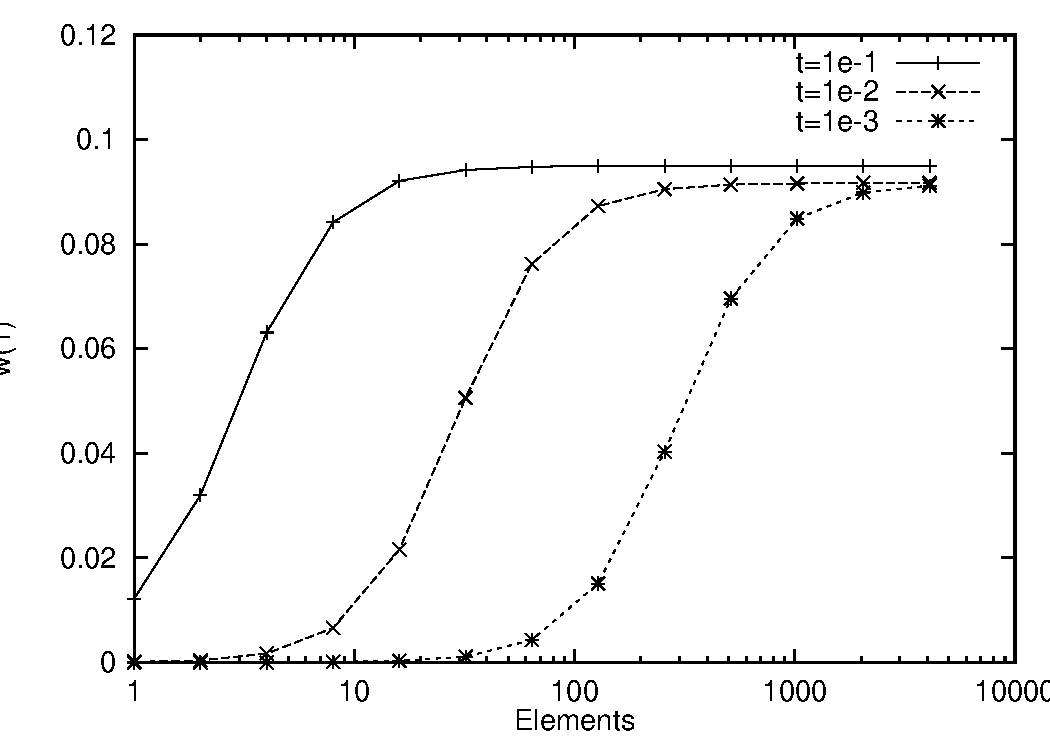
\includegraphics[width=5cm]{pictures/timowntbad}
\hspace{2cm}
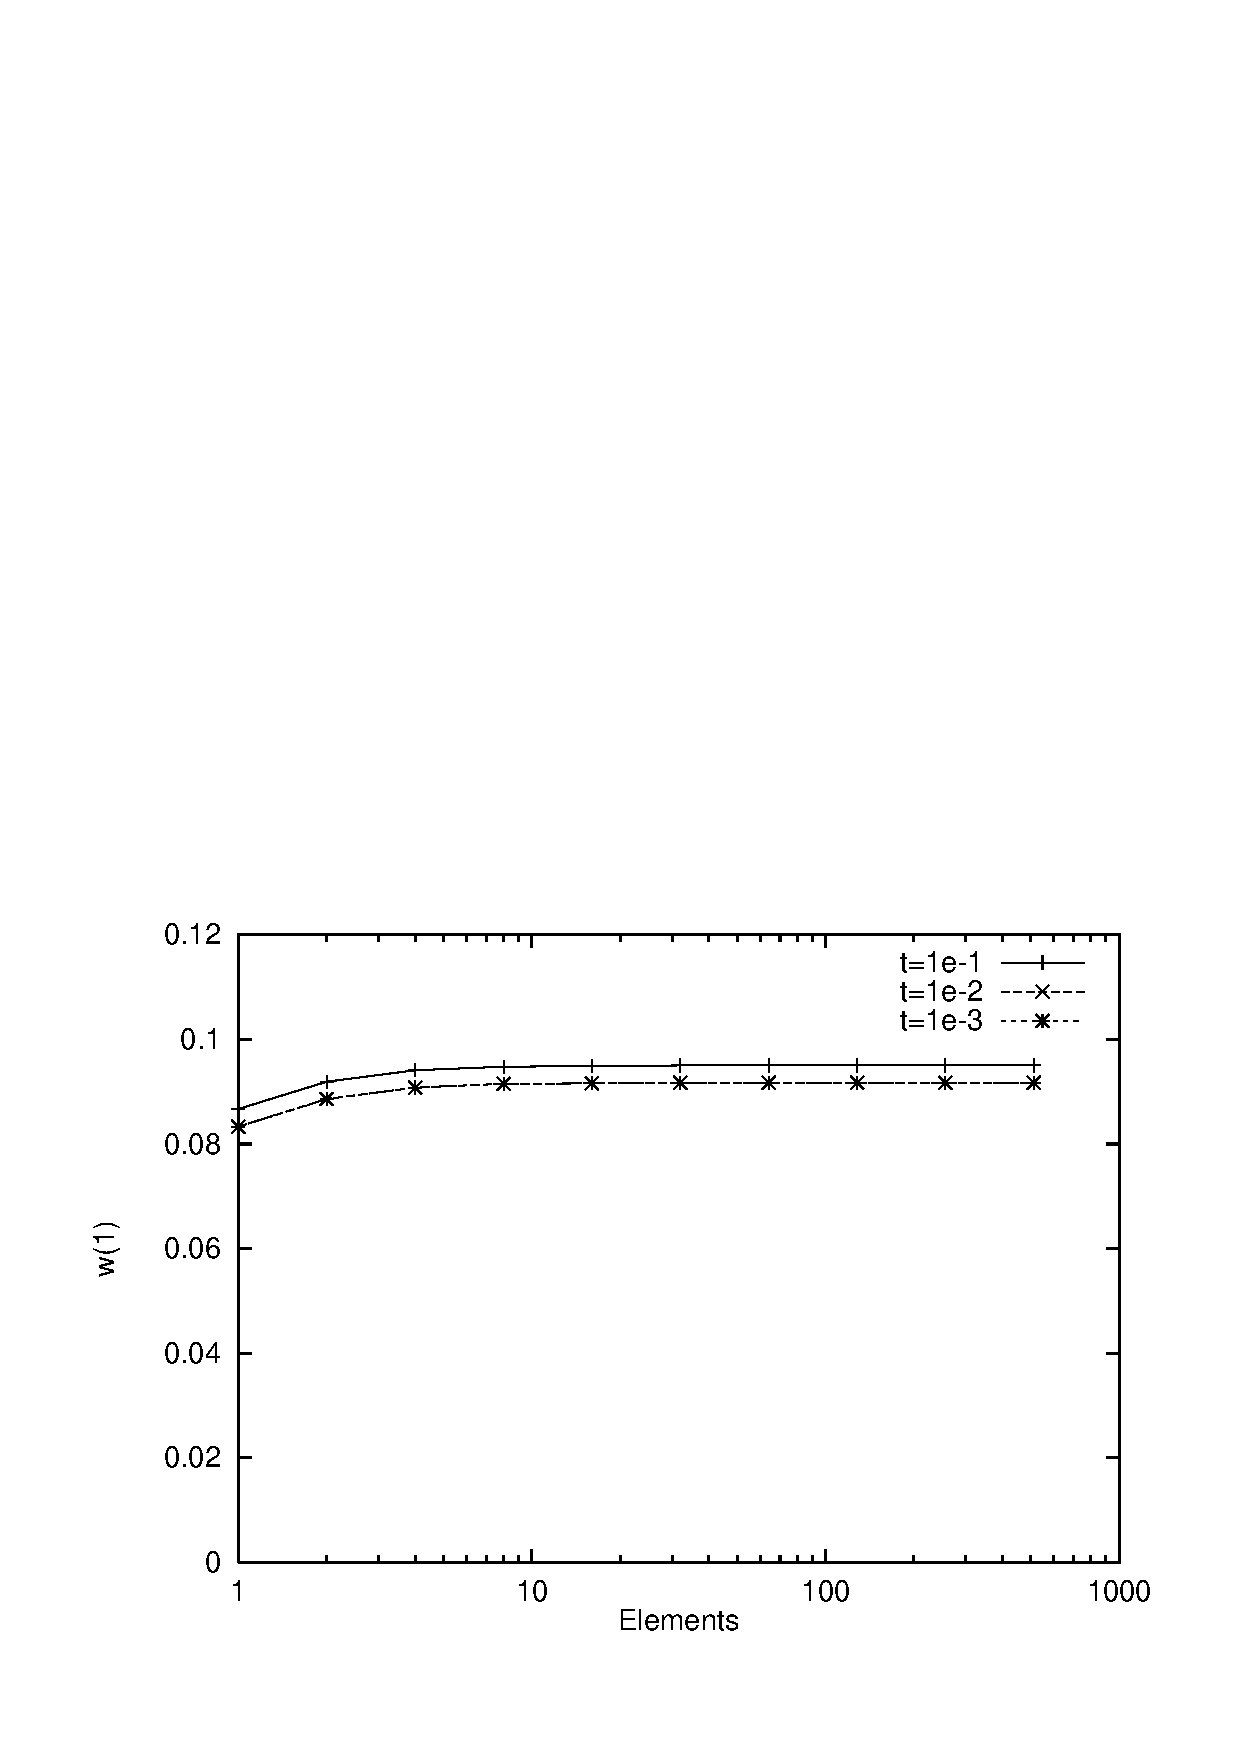
\includegraphics[width=5cm]{pictures/timowntgood}
\end{center}


\section{Maxwell equations}
%
Maxwell equations describe electro-magnetic fields. 
We consider the special case of stationary magnetic fields. 
Maxwell equations are three-dimensional.

A magnetic field is caused by an electric current. We suppose that a current density
$$
j \in [L_2(\Omega)]^3
$$
is given. (Stationary) currents do not have sources, i.e., $\opdiv \, j = 0$. 

The involved (unknown) fields are 
\begin{itemize}
\item
The magnetic flux $B$  (in German: Induktion). The flux is free of sources, i.e.,
$$
\opdiv \, B = 0.
$$
\item 
The magnetic field intensity $H$ (in German: magnetische Feldst\"arke). The field
is related to the current density by Henry's law: 
$$
\int_S j \cdot n \, ds = \int_{\partial S} H \cdot \tau \, ds  \qquad \forall \; \mbox{Surfaces } S
$$
\end{itemize}

By Stokes\'{} Theorem, one can derive Henry's law in differential form:
$$
\opcurl \, H = j
$$
The differential operator is  $\opcurl = \operatorname {rot} = \nabla \times$.
Both fields are related by a material law. The coefficient $\mu$ is called permeability:
$$
B = \mu H
$$

The coefficient $\mu$ is $10^3$ to $10^4$ times larger in iron (and other ferro-magnetic
metals) as in most other media (air). In a larger range, the function $B(H)$ is also highly
non-linear.

Collecting the equations we have
\begin{equation}
\label{equ_bhsystem}
\opdiv \, B = 0 \qquad B = \mu H \qquad \opcurl \, H = j
\end{equation}
In principle, Maxwell equations are valid in the whole $\setR^3$. For simulation, we have
to truncate the domain and have to introduce  artificial boundary conditions.

The picture below shows the magnetic field caused by a tangential current density in
a coil:
\begin{center}
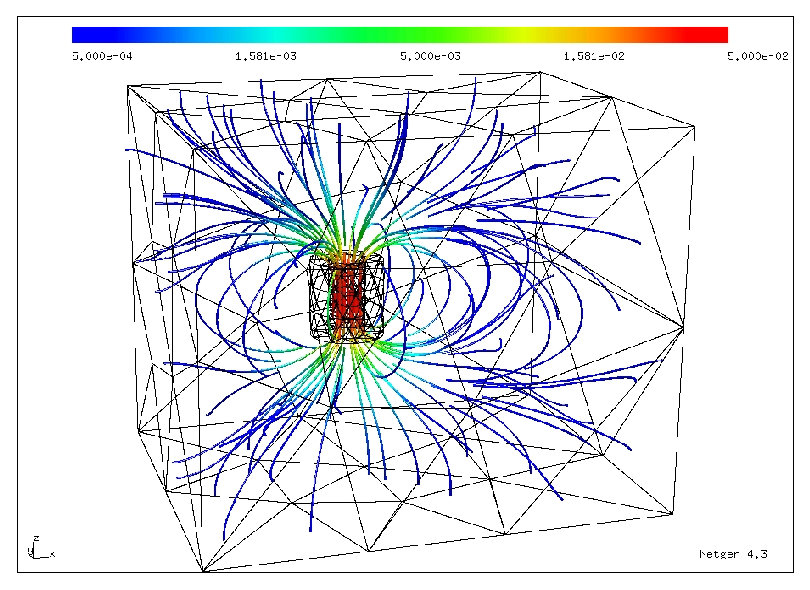
\includegraphics[width=10cm]{pictures/d7_fieldlines}
\end{center}


Compare these equations to the diffusion equation $-\opdiv \, a \nabla u = f$. Here,
we could introduce new unknowns $g = \nabla u$ and $\sigma = a g$. On simply connected
domains, $g$ is a gradient field if and only if $\opcurl g = 0$. We could reformulate
the equations as: Find vector fields $g$ and $\sigma$ such that
$$
\opcurl \, g = 0 \qquad \sigma = a g \qquad \opdiv \, \sigma = -f.
$$

The system of magnetostatic equations looks similar. Only, the right hand side data is
applied to the $\opcurl$-equation, instead of the $\opdiv$-equation. In a similar way as
$\opcurl \, g = 0$ allows to introduce a scalar field $u$ such that $g = \nabla u$,
$\opdiv \, B = 0$ allows to introduce a vector potential $A$ such that
$$
B = \opcurl \, A.
$$
Inserting the vector-potential into the equations (\ref{equ_bhsystem}), one obtains
the second order equation
\begin{equation}
\label{equ_vecpotstrong}
\opcurl \, \mu^{-1}  \opcurl A = j.
\end{equation}

The two original fields $B$ and $H$ can be obtained from the vector potential $A$.

The vector-potential $A$ is not uniquely defined by (\ref{equ_vecpotstrong}). One
may add a gradient field to $A$, and the equation is still true. To obtain a unique
solution, the so called Coloumb-Gauging can be applied:
\begin{equation}
\label{equ_divastrong}
\opdiv \, A = 0.
\end{equation}

As usual, we go over to the weak form. Equations (\ref{equ_vecpotstrong}) and
(\ref{equ_divastrong}) together become: Find $A$ such that
$$
\int_\Omega \mu^{-1} \opcurl A \, \opcurl v \, dx = \int_\Omega j \cdot v \, dx \qquad \forall \, v \in ?
$$
and
$$
\int_\Omega A \cdot \nabla \psi \, dx = 0.
$$

We want to choose the same space for $A$ and the according test functions $v$. But,
then we have more equations than unknowns. The system is still solvable, since we
have made the assumption $\opdiv \, j = 0$, and thus $j$ is in the range of the $\opcurl$-
operator. To obtain a symmetric system, we add a new scalar variable $\varphi$.
The problem is now: Find $A \in V = ?$ and $\varphi \in Q = H^1 / \setR$ such that
\begin{equation} \label{equ_vecpotmixed}
\begin{array}{ccccll}
\int \mu^{-1} \opcurl A \, \cdot \opcurl v \, dx & + & 
\int \nabla \varphi \cdot v \, dx & = & 
\int j \cdot v \, dx \qquad & \forall \, v \in V \\[0.5em]
\int A \cdot \nabla \psi \, dx & & & = & 0 & \forall \, \psi \in Q
\end{array}
\end{equation}

The proper space $V$ is the $H(\opcurl)$: 
$$
H(\opcurl) = \{ v \in [L_2(\Omega)]^3 : \opcurl \, v  \in [L_2(\Omega)]^3 \}
$$
Again, the differential operator $\opcurl$ is understood in the weak sense.
The canonical norm is
$$
\| v \|_{H(\opcurl)} = \left\{ \| v \|_{L_2}^2 + \| \opcurl \, v \|_{L_2}^2 \right\}^{1/2}.
$$

Similar to $H^1$ and $H(\opdiv)$, there exists a trace operator for $H(\opcurl)$. Now,
only the tangential components of the boundary values are well defined:

\begin{theorem} [Trace theorem] There exists a tangential trace operator $\optr_\tau v : H(\opcurl) \rightarrow W(\partial \Omega)$ such that
$$
\optr_\tau v = (v|_{\partial \Omega})_\tau
$$
for smooth functions $v \in [C(\overline \Omega)]^3$. 
\end{theorem}

\begin{theorem} Let $\Omega = \cup \Omega_i$. Assume that $u|_{\Omega_i} \in H(\opcurl,\Omega_i)$,
and the tangential traces are continuous across the interfaces $\gamma_{ij}$. Then $u \in H(\opcurl, \Omega)$.
\end{theorem}


The theorems are according to the ones we have proven for $H(\opdiv)$. But, the proofs (in $\setR^3$) are more involved.

\bigskip

The gradient operator $\nabla$ relates the space $H^1$ and $H(\opcurl)$:
$$
\nabla : H^1 \rightarrow H(\opcurl)
$$

Furthermore, the kernel space
$$
H^0(\opcurl) = \{ v \in H(\opcurl) : \opcurl \, v = 0 \}
$$
is exactly the range of the gradient:
$$
H^0(\opcurl) = \nabla \, H^1
$$



\begin{theorem} The mixed system (\ref{equ_vecpotmixed}) is a well posed problem
on $H(\opcurl) \times H^1/\setR$.
\end{theorem}
{\em Proof:} The bilinear-forms
$$
a(A,v) = \int \mu^{-1} \opcurl A \cdot \opcurl v \, dx
$$
and 
$$
b(v, \varphi) = \int v \cdot \nabla \varphi \, dx
$$
are continuous w.r.t. the norms of $V = H(\opcurl)$ and $Q = H^1/\setR$. 

The LBB-condition in this case is trivial. Choose $v = \nabla \varphi$:
$$
\sup_{v \in H(\opcurl)} \frac{ \int v \nabla \varphi \, dx } { \| v \|_{H(\opcurl)}}
\geq \frac{ \int \nabla \varphi \cdot \nabla \varphi \, dx } { \| \nabla \varphi \|_{H(\opcurl)}}
= \frac{ \| \nabla \varphi \|_{L_2}^2 } { \| \nabla \varphi \|_{L_2}} = \| \nabla \varphi \|_{L_2} \eqc \| \varphi \|_Q
$$

The difficult part is the kernel coercivity of $a(.,.)$. 
The norm involves also the $L_2$-norm, while the bilinear-form only involves the semi-norm
$\| \opcurl \, v \|_{L_2}$. Coercivity cannot hold on the whole $V$: Take a gradient function
$\nabla \psi$. On the kernel, the $L_2$-norm is bounded by the semi-norm:
$$
\| v \|_{L_2} \leqc \| \opcurl \, v \| \qquad \forall \, v \in V_0,
$$
where
$$
V_0 = \{ v \in H(\opcurl) :  \int v \nabla \varphi \, dx = 0 \; \; \forall \, \varphi \in H^1 \}
$$
This is a Friedrichs-like inequality.


\subsubsection{Finite elements in $H(\opcurl)$}
%
We construct finite elements in three dimensions.
The trace theorem implies that functions in $H(\opcurl)$ have continuous tangential 
components across element boundaries (=faces). 

\bigskip

We design tetrahedral finite elements.
The pragmatic approach is to choose the element space as $V_T = P^1$, and choose the 
degrees of freedom as the 
tangential component along the edges in the end-points of the edges. The dimension of
the space is $3 \times \mbox{dim} \{ P^1 \} = 3 \times 4 = 12$, the degrees of freedom
are 2 per edge, i.e., $2 \times 6 = 12$. They are also linearly independent. In each
face, the tangential component has 2 components, and is linear. Thus, the tangential
component has dimension 6. These 6 values are defined by the 6 degrees of freedom of the
3 edges in the face. Neighboring elements share this 6 degrees of freedom in the face,
and thus have the same tangential component.

\bigskip

There is a cheaper element, called N{\'e}d{\'e}lec, or edge-element. 
It has the same accuracy for the $\opcurl$-part (the $B$-field)  as the $P^1$-element. 
It is similar to the Raviart-Thomas element. It contains all constants, 
and some linear polynomials. All 3 components are defined in common. The element space is
$$
V_T = \{ a + b \times x : a, b \in \setR^3 \}.
$$
These are 6 coefficients. For each of the 6 edges of a tetrahedron, one chooses the
integral of the tangential component along the edge
$$
\psi_{E_i}(u) = \int_{E_i} u \cdot \tau_{E_i} \, ds.
$$
\begin{lemma} The basis function $\varphi_{E_i}$ associated with the edge $E_i$ is
$$
\varphi_{E_i} = \lambda_{E_i^1} \nabla \lambda_{E_i^2} - \nabla \lambda_{E_i^2} \lambda_{E_i^1},
$$
where $E_i^1$ and $E_i^2$ are the two vertex numbers of the edge, and $\lambda_1, \ldots \lambda_4$
are the vertex shape functions.
\end{lemma}
{\em Proof: } \begin{itemize}
\item These functions are in $V_T$
\item If $i \neq j$, then $\psi_{E_j}(\varphi_{E_i}) = 0$.
\item $\psi_{E_i}(\varphi_{E_i}) = 1$
\end{itemize}

Thus, edge elements belong to $H(\opcurl)$. Next, we will see that they have also very
interesting properties.

\subsubsection{The de'Rham complex}

The spaces $H^1$, $H(\opcurl)$, $H(\opdiv)$, and $L_2$ form a sequence:

$$
\begin{array}{ccccccc}
H^1             &      \stackrel{\nabla}{\longrightarrow}          &
H(\opcurl)      &      \stackrel{\opcurl}{\longrightarrow}   &
H(\opdiv)       &      \stackrel{\opdiv}{\longrightarrow}    & 
L^2                                                                                    
\end{array}
$$

Since $\nabla H^1 \subset [L_2]^3$, and $\opcurl \nabla = 0$, the gradients 
of $H^1$ functions belong to $H(\opcurl)$. 
Similar, since $\opcurl H(\opcurl) \subset [L_2]^3$, and $\opdiv \opcurl = 0$, 
the $\opcurl$s of $H(\opcurl)$ functions belong to $H(\opdiv)$.

The sequence is a {\em complete} sequence. This means that the kernel of the right
differential operator is exactly the range of the left one (on simply connected domains). 
We have used this property
already in the analysis of the mixed system.

The same property holds on the discrete level: Let \\
\begin{center}
\begin{tabular}{cl}
$W_h$ & be the nodal finite element sub-space  of $H^1$ \\
$V_h$ & be the N\'ed\'elec (edge) finite element sub-space of $H(\opcurl)$ \\
$Q_h$ & be the Raviart-Thomas (face) finite element sub-space of $H(\opdiv)$ \\
$S_h$ & be the piece-wise constant finite element sub-space of $L_2$
\end{tabular}
\end{center}

\begin{theorem}
The finite element spaces form a complete sequence
$$
\begin{array}{ccccccc}
W_h             &      \stackrel{\nabla}{\longrightarrow}          &
V_h             &      \stackrel{\opcurl}{\longrightarrow}   &
Q_h             &      \stackrel{\opdiv}{\longrightarrow}    & 
S_h                                                                                    
\end{array}
$$
\end{theorem}


Now, we discretize the mixed formulation (\ref{equ_vecpotmixed}) by choosing
edge-finite elements for $H(\opcurl)$, and nodal finite elements for $H^1$: Find
$A_h \in V_h$ and $\varphi_h \in W_h$ such that
\begin{equation} \label{equ_vecpotmixedh}
\begin{array}{ccccll}
\int \mu^{-1} \opcurl A_h \, \cdot \opcurl v_h \, dx & + & 
\int \nabla \varphi_h \cdot v_h \, dx & = & 
\int j \cdot v_h \, dx \qquad & \forall \, v_h \in V_h \\[0.5em]
\int A_h \cdot \nabla \psi_h \, dx & & & = & 0 & \forall \, \psi_h \in W_h
\end{array}
\end{equation}
The stability follows (roughly) from the discrete sequence property. The verification
of the LBB condition is the same as on the continuous level. The kernel of the $a(.,.)$-
form are the discrete gradients, the kernel of the $b(.,.)$-form is orthogonal to
the gradients. This implies solvability. The discrete kernel-coercivity (with $h$-independent
constants) is true (nontrivial).


\bigskip


The complete sequences on the continuous level and on the discrete level are connected
in the de'Rham complex: Choose the canonical interpolation operators 
(vertex-interpolation $I^W$, edge-interpolation $I^V$, face-interpolation $I^Q$, 
$L_2$-projection $I^S$). This relates the continuous level to the discrete level:

\begin{equation}
\begin{array}{ccccccc}
H^1             &      \stackrel{\nabla}{\longrightarrow}          &
H(\opcurl)      &      \stackrel{\opcurl}{\longrightarrow}   &
H(\opdiv)       &      \stackrel{\opdiv}{\longrightarrow}    & 
L^2                                                                                    \\[8pt]
\Big\downarrow  \vcenter{ \rlap{$I^W$}}  &                  &
\Big\downarrow  \vcenter{ \rlap{$I^V$}}  &                  &
\Big\downarrow  \vcenter{ \rlap{$I^Q$}}  &                  &
\Big\downarrow  \vcenter{ \rlap{$I^S$}}                             \\[8pt]
 W_h                   &      
\stackrel{\nabla}{\longrightarrow}          &
 V_h       &     
 \stackrel{\opcurl}{\longrightarrow}   &
 Q_h          &      
\stackrel{\opdiv}{\longrightarrow}    & 
S_h  \:.                                                                               \\[8pt]
\end{array}
\label{equ_derham}
\end{equation}

\begin{theorem}
The diagram (\ref{equ_derham}) {\em commutes}:
$$
I^V \nabla = \nabla I^W \qquad
I^Q \opcurl = \opcurl I^V \qquad
I^S \opdiv = \opdiv I^Q
$$
\end{theorem}
{\em Proof:} We prove the first part. Note that the ranges of both,
$\nabla I^W$ and $I^V \nabla$, are in $V_h$. Two functions in $V_h$ coincide if
and only if all functionals coincide. It remains to prove that
$$
\int_E (\nabla I^W w) \cdot \tau \, ds = \int_E (I^V \nabla w)\cdot \tau \, ds
$$
Per definition of the interpolation operator $I^V$ there holds
$$
\int_E (I^V \nabla w)\cdot \tau \, ds = \int_E \nabla w \cdot \tau \, ds
$$
Integrating the tangential derivative gives the difference
$$
\int_E \nabla w \cdot \tau \, ds = \int_E \frac{\partial w}{\partial \tau} \, ds = w(E^2) - w(E^1)
$$
Starting with the left term, and using the property of the nodal interpolation operator,
we obtain
$$
\int_E (\nabla I^W w) \cdot \tau \, ds = (I^W w)(E^2) - (I^W w)(E^1) = w(E^2) - w(E^1).
$$
We have already proven the commutativity of the $H(\opdiv)-L_2$ part of the diagram.
The middle one involves Stokes\'{} theorem.
\hfill $\Box$


This is the key for interpolation error estimates. E.g., in $H(\opcurl)$ there holds
\begin{eqnarray*}
\| u - I^V u \|_{H(\opcurl)}^2 
& = & \| u - I^V u \|_{L_2}^2 + \| \opcurl (I-I^V) u \|_{L_2}^2 \\
& = & \| u - I^V u \|_{L_2}^2 + \| (I-I^Q) \opcurl u \|_{L_2}^2 \\
& \leqc & h^2 \, \| u \|_{H^1}^2 + h^2 \| \opcurl u \|_{H^1}^2 
\end{eqnarray*}
Since the estimates for the $L_2$-term and the $\opcurl$-term are separate, one can
also scale each of them by an arbitrary coefficient.

\bigskip

The sequence is also compatible with transformations. Let $F : \widehat T \rightarrow T$
be an (element) transformation. Choose
\begin{eqnarray*}
w(F(x)) & = & \hat w(x) \\
v(F(x)) & = & (F^\prime)^{-T} \hat v(x) \qquad \qquad \quad \, \mbox{(covariant transformation)}\\
q(F(x)) & = & (\opdet{F^\prime})^{-1} (F^\prime) q(x) \qquad \mbox{(Piola-transformation)} \\
s(F(x)) & = & (\opdet{F^\prime})^{-1} \hat s(x)
\end{eqnarray*}
Then 
\begin{eqnarray*}
\hat v = \nabla \hat w & \Rightarrow & v = \nabla  \, w \\
\hat q = \opcurl \hat v & \Rightarrow & q = \opcurl \, v \\
\hat s = \opdiv \hat q & \Rightarrow & s = \opdiv \, q
\end{eqnarray*}
Using these transformation rules, the implementation of matrix assembling for 
$H(\opcurl)$-equations is very similar to the assembling for $H^1$ problems
(mapping to reference element).




\chapter{Parabolic partial differential equations}

PDEs involving first order derivatives in time, and an ellitpic differential operator
in space, are called parabolic PDEs. For example, time dependent heat flow is described
by a parabolic PDE.

Let $\Omega \subset \setR^d$, and $Q = \Omega \times (0,T)$. Consider the initial-boundary
value problem
$$
\frac{\partial u(x,t)}{\partial t} - \opdiv (a(x) \nabla_x u(x,t)) = f(x,t)  \qquad (x,t) \in Q,
$$
with boundary conditions
\begin{eqnarray*}
u(x,t) & = & u_D (x,t) \qquad (x,t) \in \Gamma_D \times (0,T), \\
a(x) \frac{\partial u}{\partial n} & = & g(x,t) \; \; \qquad (x,t) \in \Gamma_N \times (0,T),
\end{eqnarray*}
and initial conditions
$$
u(x,0) = u_0(x) \qquad x \in \Omega.
$$

\bigskip

Weak formulation in space: Find $u : [0,T] \rightarrow H_{0,D}^1(\Omega)$ such that
\begin{eqnarray*}
\int_\Omega \partial_t u (x,t) v(x) \, dx + 
\int_\Omega a \nabla u(x,t) \cdot \nabla v(x,t) \, dx & = &
\int_\Omega f(x,t) v(x,t) \, dx + \int_{\Gamma_N} g(x,t) v(x,t) \, dx \\[1em]
& &  \forall \, v \in H_{0,D}^1, \; t \in (0,T]
\end{eqnarray*}
In abstact form: Find $u : [0,T] \rightarrow V$ s.t.
$$
(u^\prime(t), v)_{L_2} + a(u(t), v) = \left< f(t), v \right> \qquad \forall \, v \in V, \, t \in (0,T]
$$
In operator form (with $\left<A u,v\right> = a(u,v)$):
$$
u^\prime (t) + A u(t) = f(t)  \qquad \in V^\ast
$$
\bigskip
Function spaces:
$$
X = L_2( (0,T), V) \qquad X^\ast = L_2((0,T), V^\ast)
$$
with norms
$$
\| v  \|_X = \left( \int_0^T \| v(t) \|_V^2 \, dt \right)^{1/2}
\qquad
\| v  \|_{X^\ast} = \left( \int_0^T \| v(t) \|_{V^\ast}^2 \, dt \right)^{1/2}
$$

\begin{definition} Let $u \in L_2( (0,T), V)$. It has a weak derivative 
$w \in L_2((0,T),V^\ast)$ if
$$
\int_0^T \varphi(t) \left< w, v \right>_{V^\ast \times V} \, dt = -\int_0^T \varphi^\prime (t) (u,v)_{L_2} \, dt 
\qquad \forall \, v \in V, \; \forall \, \varphi \in C_0^\infty (0,T)
$$
\end{definition}

\begin{definition} 
$$
H^1 ((0,T),V;L_2) = \{ v \in L_2((0,T),V) : v^\prime \in L_2((0,T),V^\ast) \}
$$
with norm
$$
\| v \|_{H^1}^2 = \| v \|_X^2 + \| v^\prime \|_{X^\ast}^2.
$$
\end{definition}

This space is a one-dimensional Sobolev space with range in a Hilbert space.

\begin{theorem}[Trace theorem]
Point evaluation is continuous:
$$
\max_{t \in [0,T]} \| v(t) \|_{L_2} \leqc \| v\|_{H^1}
$$
\end{theorem}
This allows the formulation of the initial value $u(0) = u_0$.

\begin{theorem} Assume that $a(.,.)$ is 
coercive
$$
a(u,u) \geq \mu_1 \| u \|_V^2 \quad \forall \, u \in V
$$
and continuous
$$
a(u,v) \leq \mu_2 \|u \|_V \, \| v\|_V \qquad \forall \, u,v \in V.
$$ 
Then, the parabolic problem has a unique solution depending continuously on the 
right hand side and the initial conditions:
\begin{eqnarray*}
 \| u \|_{H^1((0,T),V; L_2)} & \leqc & \| u_0 \|_{L_2} + \| f \|_{L_2((0,T),V^\ast}.
\end{eqnarray*}
\end{theorem}
We only prove stability: Choose test functions $v = u(t)$:
$$
(u^\prime(t), u(t))_{L_2} + a(u(t), u(t)) = \left< f(t), u(t) \right>
$$
Use that
$$
\frac{d}{dt} \| u(t) \|_{L_2}^2 = 2 (u^\prime(t), u(t))_{L_2},
$$
and integrate the equation over $(0,T)$:
\begin{eqnarray*}
\frac{1}{2} \left\{ \| u(T) \|_{L_2}^2 - \| u_0 \|_{L_2}^2 \right\}
& = & \int_0^T \left< f(s), u(s) \right> - a(u(s), u(s)) \, ds \\
& \leq &  \int_0^T \| f(s) \|_{V^\ast} \| u(s) \|_V - \mu_1 \| u(s) \|_V^2 \; ds \\
& \leq & \| f \|_{X^\ast} \| u \|_X - \mu_1 \| u \|_X^2
\end{eqnarray*}
Since $\| u(T) \| \geq 0$, one has
$$
\mu_1 \| u \|_X^2 - \| f \|_{X^\ast} \| u \|_X \leq \frac{1}{2} \, \| u_0 \|_{L_2}
$$
Solving the quadatic inequality, one obtains the bound
$$
\| u \|_X \leq \frac{1}{2\mu_1} \left\{ \| f \|_{X^\ast} + \sqrt{\| f \|_{X^\ast}^2 + 2 \mu_1 \| u_0 \|_{L_2}^2} \right\}
$$
The bound $\| u^\prime \|_{L_2((0,T),V^\ast)}$ follows from $u^\prime(t) = f(t) - A u(t)$.

\section{Semi-discretization}
We start with a discretization in space. Choose a (finite element) sub-space $V_h \subset V$.
The Galerkin discretiztaion is: Find $u : [0,T] \rightarrow V_h$ such that
$$
(u_h^\prime(t), v_h)_{L_2} + a(u_h(t), v_h) = \left<f(t), v_h\right> 
\qquad \forall \, v_h \in V_h, \; \forall \, t \in (0,T],
$$
and initial conditions
$$
(u_h(0), v_h)_{L_2} = (u_0, v_h)_{L_2} \qquad \forall \, v_h \in V_h.
$$
Choose a basis $\{ \varphi_1, \ldots \varphi_N \}$ of $V_h$. Expand the solution w.r.t. this
basis:
$$
u_h(x,t) = \sum_{i=1}^N u_i(t) \varphi_i(x),
$$
and choose test functions $v = \varphi_j$. With the matrices
$$
M = \left( (\varphi_j, \varphi_i)_{L_2} \right)_{i,j=1,\ldots, N} \qquad
A = \left( a(\varphi_j, \varphi_i) \right)_{i,j=1,\ldots, N},
$$
and the $t$-dependent vector
$$
f(t) = \left( \left<f(t), \varphi_j\right> \right)_{i=1,\ldots,N},
$$
one obtains the system of ordinary differential equations (ODEs)
$$
M u^\prime (t) + A u(t) = f(t), \qquad u(0) = u_0
$$

In general, the (mass) matrix $M$ is non-diagonal. In the case of the (inexact) 
vertex integration rules, or non-conforming $P_1$-elements, $M$ is a diagonal matrix.
Then, this ODE can be efficiently reduced to explicit form
$$
u^\prime(t) + M^{-1} A u(t) = f(t)
$$

\bigskip

\begin{theorem}
There holds the error estimate
$$
\| u - u_h \|_{H^1((0,T),V;L_2)} \leqc  \| (I-R_h) u \|_{H^1((0,T),V;L_2)},
$$
where $R_h$ is the Ritz projector
$$
R_h : V \rightarrow V_h : \qquad a(R_h u, v_h) = a(u,v_h) \qquad \forall \, u \in V, \forall \, v_h \in V_h.
$$
\end{theorem}
{\em Proof:} 
The error is split into two parts:
$$
u(t) - u_h(t) = \underbrace{u(t)-R_h u(t)}_{\rho(t)} + \underbrace{R_h u(t) - u_h(t)}_{\Theta_h}
$$
The first part, $u(t) - R_h u(t)$ is the elliptic discretization error, which can be bounded by
Cea's lemma. To bound the second term, we use the properties for the continuous and the
discrete formulation:
\begin{eqnarray*}
\left<f,v_h\right> & = & (u^\prime,v_h) + a(u, v_h) = (u^\prime,v_h) + a(R_h u, v_h) \\
& = & (u_h^\prime, v_h) + a(u_h, v_h),
\end{eqnarray*}
i.e.,
$$
(u^\prime - u_h^\prime, v_h) + a(R_h u - u_h, v_h) = 0,
$$
or
$$
(R_h u^\prime - u_h^\prime, v_h) + a(R_h u - u_h, v_h) = (R_h u^\prime - u^\prime, v_h).
$$
With the abbreviations from above we obtain the discrete parabolic equation for $\Theta_h$:
\begin{eqnarray*}
(\Theta_h^\prime, v_h) + a (\Theta_h, v_h) & = & (\rho^\prime, v_h)  \\
\Theta_h(0) & = & (I-R_h) u(0).
\end{eqnarray*}
The stability estimate, and the trace theorem bounds
\begin{eqnarray*}
\| \Theta_h \|_{H^1((0,T),V;L_2)}
 & \leqc &  \| (I-R_h) u(0) \|_{L_2(\Omega)} + \| \rho^\prime \|_{L_2((0,T),V^\ast)} \\
 & \leqc & \| (I-R_h) u \|_{H^1((0,T),V;L_2)}
\end{eqnarray*}
\hfill $\Box$

\section{Time integration methods}
Next, we discuss methods for solving the system of ODEs:
\begin{eqnarray}
M u^\prime(t) + A u(t) & = & f(t) \label{equ_ode} \\
u(0) & = & u_0  \nonumber
\end{eqnarray}
We focus on simple time integration rules and the specific properties arising from
the space-discretization of parabolic PDEs. Let 
$$
0 = t_0 < t_1 < t_m = T,
$$
a partitioning of the interval $[0,T]$. Define $\tau_j = t_{j+1}-t_j$.
Integrating (\ref{equ_ode}) over the intervalls leads to
$$
M \left\{ u(t_{j+1}) - u(t_j)  \right\} + \int_{t_j}^{t_{j+1}} A u(s) \, ds = \int_{t_j}^{t_{j+1}} f(s) \, ds.
$$

Next, we replace the integrals by numerical integration rules. The left-sided rectangle rule
leads to
$$
M \{ u(t_{j+1}) - u(t_j) \} + \tau_j A u(t_j) = \tau_j f(t_j)
$$
With the notation $u_j = u(t_j)$, this leads to the sequence of linear equations
$$
M u_{j+1} = M u_j + \tau_j (f_j - A u_j)
$$
In the case of a diagoal $M$-matrix, this is an explicit formulae for the new time step !

Using the right-sided rectangle rule leads to
$$
M \{ u_{j+1} - u_j \} + \tau_j A u_{j+1} = \tau_j f_{j+1},
$$
or
$$
(M + \tau_j A) u_{j+1} = M u_j + \tau_j f_{j+1}.
$$
In case of the right-side rule, a linear system must be solve in any case. Thus,
this method is called an implicit time integration method. These two special cases
are called the explicit Euler method, and the implicit Euler method. A third simple
choice is the trapezoidal rule leading to
$$
(M + \frac{\tau_j}{2} A) u_{j+1} = M u_j + \frac{\tau_j}{2} (f_j+f_{j+1} - A u_j)
$$
It is also an implcit method. Since the trapezoidal integration rule is more accurate,
we expect a more accurate method for approximating the ODE.



All single-step time integration methods can be written in the form
$$
u_{j+1} = G_j (u_j, f_j),
$$
where $G_j$ is linear in both arguments and shall be continuous with bounds
$$
\| G_j (u_j, f_j) \|_M \leq L \, \| u_j \|_M + \tau_j \, l \, \| f_j \|_{M^{-1}},
$$
with $L \geq 1$.
\begin{lemma}
The time integration method fulfills the stability estimate
\begin{equation}
\| u_j \|_M \leq L^j \, \| u_0 \|_M + l L^j \sum_{i=0}^{j-1} \tau_i \| f_i \|_{M^{-1}}
\end{equation}
\end{lemma}

The explicit Euler method is written as
$$
u_{j+1} = (I - \tau M^{-1} A) u + \tau M^{-1} f_j,
$$
and has bounds
\begin{eqnarray*}
L & = & \max \{ 1, \tau \lambda_{max} (M^{-1} A)-1 \} \eqc \max\{ 1, \frac{\tau}{h^2} \}\\
l & = & 1
\end{eqnarray*}

If $\tau > h^2$, the powers $L^j$ become very large. This means that the explicit Euler
method becomes instable. Thus, for the explicit Euler method, the time-step $\tau$
must not be greater than $c h^2$.

The implicit Euler method is written as
$$
u_{j+1} = (M + \tau A)^{-1} M u_j + \tau (M+\tau A)^{-1} f_j,
$$
and has the bounds
\begin{eqnarray*}
L & = & 1 \\
l & = & 1
\end{eqnarray*}
The method is stable for any time-step $\tau$. Such a method is called $A$-stable.

\begin{lemma} The time discretization error $e_j := u(t_j) - u_j$ of the
implicit Euler method satisfies the difference equation
$$
M \{ e_{j+1} - e_j \} + \tau A e_{j+1} = d_j,
$$
where the $d_j$ satisfy
$$
d_j = \int_{t_j}^{t_{j+1}} \{ f(s) - A u(s) \} \, ds - \tau_j \{ f(t_{j+1}) - A u(t_{j+1}) \}.
$$
\end{lemma}

\begin{lemma} The  error of the integration rule can be estimated by
$$
\| d_j \| \leqc \tau \, \| (f - A u)^\prime \|_{L_\infty} = \tau \, \| u^{\prime \prime} \|_{L_\infty}
$$
\end{lemma}

Convergence of the time-discretization method follows from stability plus 
approximation:
\begin{theorem} The error of the implicit Euler method satisfies
$$
\| u(t_j) - u_j \|_M \leq \sum_{i=0}^j \tau \| d_j \| \leqc \tau \, \| u^{\prime \prime} \|_{L_\infty(0,T)}
$$
\end{theorem}

\bigskip
The trapezoidal rule is $A$-stable, too. It is based on a more accurate integration
rule, and leads to second order convergence $O(\tau^2)$.
Convergence of higher order can be obtained by Runge-Kutta methods. 


% \documentclass[12pt]{article}
% \usepackage{amsmath,amsthm,amssymb,a4wide}
% \usepackage[german,english]{babel}
% \usepackage{epsfig}
% \usepackage{latexsym}
% \usepackage{amssymb}
% % \usepackage{theorem}
% \usepackage{amsthm}
% % \usepackage{showkeys}

% \newcommand{\setR}{ {\mathbb R} }
% \newcommand{\setN}{ {\mathbb N} }
% \newcommand{\setZ}{ {\mathbb Z} }
% \newcommand{\eps}{\varepsilon}

% \newcommand{\beq}{\begin{equation}}
% \newcommand{\eeq}{\end{equation}}

% \newcommand{\opdiv}{\operatorname{div}}
% \newcommand{\opcurl}{\operatorname{curl}}
% \newcommand{\opdet}{\operatorname{det}}
% \newcommand{\optr}{\operatorname{tr}}
% \newcommand{\optrn}{\operatorname{tr}_n}
% \newcommand{\sfrac}[2]{ { \textstyle \frac{#1}{#2} } }

% \newcommand{\Zh}{\mathrm{Z}_h}
% \newcommand{\Ih}{\mathrm{I}_l}

% \newcommand{\leqc}{\preceq} 
% \newcommand{\geqc}{\succeq} 
% \newcommand{\eqc}{\simeq} 
% \newcommand{\ul}{\underline}

% \newtheorem{theorem}{Theorem}
% \newtheorem{definition}[theorem]{Definition}
% \newtheorem{lemma}[theorem]{Lemma}
% \newtheorem{remark}[theorem]{Remark}
% \newtheorem{example}[theorem]{Example}

% %
% %
% \setlength{\unitlength}{1cm}
% \sloppy 
% %

% \title{Space-time formulation of Parabolic Equations}
% \author{Joachim Sch\"oberl}

% \begin{document}
% \maketitle
% \centerline{(supplement to lecture notes Chapter 9, draft version) } 

\section{Space-time formulation of Parabolic Equations}

In the previous section we have discretized in space to obtain an ordinary differential equation, which 
is solved by some time-stepping method. This approach is known as method of lines.
Now we formulate a space-time variational problem. This is discretized in time and space
by a (discontinuous) Galerkin method. We obtain time-slabs which are solved one after another.
This approach is more flexible, since it allows to use different meshes in space on different time-slabs.

\subsection{Solvability of the continuous problem}
%
Let $V \subset H$ be Hilbert spaces, typically $H = L_2(\Omega)$ and $V = H^1(\Omega)$. Duality is defined with respect to $H$.
For $t \in (0,T)$ we define the familiy $A(t) : V \rightarrow V^\ast$ of uniformely continuous and elliptic operators:
\begin{enumerate}
\item[(a)] $\left< A(t) u, u \right> \geq \alpha_1 \| u \|_V^2 $
\item[(b)] $\left< A(t) u, v \right> \leq \alpha_2 \| u \|_V  \, \| v \|_V$ 
\end{enumerate}
We assume that $\left< A(t) u, v \right>$ is integrable with respect to time. We do not assume that $A(t)$ is symmetric.
We consider the parabolic equation: Find $u : [0,T] \rightarrow V$ such that
\begin{eqnarray*}
u^\prime + A u & = & f  \quad \forall \, t \in (0,T) \\
u(0) & = & u_0
\end{eqnarray*}
We define $X = \{ v \in L_2(V) : v^\prime \in L_2(V^\ast) \} $ and $Y = L_2(V)$, with its dual $Y^\ast = L_2(V^\ast)$.
A variational formulation is: Find $u \in X$ such that
\begin{eqnarray} 
\label{equ_parabolic1}
\int_0^T \left< u^\prime + A u, v \right> & = & \int_0^T \left< f, v \right>   \qquad \forall \, v \in Y \\
\label{equ_parabolic2}
(u(0), v_0)_H & = & (u_0, v_0) \qquad \forall v_0 \in H
\end{eqnarray}

Adding up both equations leads to the variational problem $B(u,v) = f(v)$ with the bilinear-form
$B(.,.) : X \times (Y \times H) \rightarrow \setR$:
$$
B(u, (v,v_0)) = \int_0^T \left< u^\prime + A u, v \right> + (u(0), v_0)_H
$$
and the linear-form $f : Y \times H \rightarrow \setR$:
$$
f(v,v_0) = \int_0^T \left< f, v \right> + (u_0, v_0)_H
$$ 
We assume that $f \in Y^\ast$ and $u_0 \in H$

\begin{theorem}[Lions] \label{theo_continuous} Problem~(\ref{equ_parabolic1})-(\ref{equ_parabolic2}) is uniquely solvable.
\end{theorem}
\begin{proof}
We apply the theorem by Babu\v{s}ka-Aziz. We observe that all forms are continuous (trace-theorem). 
We have to verify both inf-sup conditions.

First, we show
\begin{equation}
\inf_{u \in X} \sup_{ (v,v_0) \in Y \times H} \frac{B(u,v)} {\| u \|_X  \| (v,v_0) \|_{Y \times H}}  \geq \beta > 0
\end{equation}
We fix some $u \in X$ and set (with $A^{-T}$ the inverse of the adjoint operator)
\begin{eqnarray*}
v &  := & A^{-T} u^\prime + u \\
v_0 & := & u(0)
\end{eqnarray*}
and obtain
\begin{eqnarray*}
B(u,v) & = & \int \left< u^\prime + A u, A^{-T} u^\prime + u \right> \, dt \; + (u(0), u(0))_H \\
& = & \int \left<A^{-1} u^\prime, u^\prime \right> + \left< A u, u \right> + \left< u^\prime, u \right> + \left< u, u^\prime \right> \, dt \;  + \| u_0 \|_H^2 \\
& = & \int \left<A^{-1} u^\prime, u^\prime \right> + \left< A u, u \right> + \frac{d}{dt} \| u \|_H^2  + \| u_0 \|_H^2 \\
& \geq & \alpha_2^{-1}  \| u^\prime \|^2_{L_2(V^\ast)} + \alpha_1 \| u \|^2_{L_2(V)} + \| u(T) \|_H^2 \\
& \geqc &  \| u \|_X^2
\end{eqnarray*}
Since $\| (v,v_0) \|_{Y \times H} \leqc \| u \|_X$ the first $\inf-\sup$-condition is proven.
For the other one, we show
\begin{equation}
\forall \, 0 \neq (v,v_0) \in Y \times H \; \; \exists \, u \in X  \;  : \;  B(u,v) > 0
\end{equation}
We fix some $v, v_0$. We define $u$ by solving the parabolic equation
$$
u^\prime + \gamma L u = A^T v, \qquad u(0) = v_0,
$$
where $L$ is a symmetric, constant-in-time, continuous and elliptic operator on $V$. 
The parameter~$\gamma > 0, \gamma = O(1)$ will be fixed later. The equation has a unique solution, which can be constructed by spectral theory.
If $(v,v_0) \neq 0$, then also $u \neq 0$.

\begin{eqnarray*}
B(u,v) & = & \int \left< u^\prime + A u, A^{-T} (u^\prime + \gamma L u) \right> + \| v_0\|_H^2 \\
& = & \int \left< u^\prime, A^{-T} u^\prime\right> + \left< u, u^ \prime\right> + \left< u^\prime, A^{-T } \gamma L u \right> + \gamma \left< u, L u \right> \, dt +  \| v_0 \|_H^2 \\
& \geq & \int \tfrac{1}{\alpha_2} \| u^\prime \|_{V^\ast}^2 + \tfrac{1}{2} \tfrac{d}{dt} \| u \|_H^2 - \| u^\prime \|_{V^\ast} \| A^{-T} \gamma L u \|_V + \gamma \left< u, L u \right> + \| v_0 \|_{H}^2
\end{eqnarray*}
The second term is integrated in time, and we apply Young's inequality for the negative term:
\begin{eqnarray*}
B(u,v) & \geq & \int \tfrac{1}{\alpha_2} \| u^\prime \|_{V^\ast}^2  - \tfrac{1}{2\alpha_2}\| u^\prime \|_{V^\ast}^2 - \tfrac{\alpha_2}{2} \| A^{-T} \gamma L u \|_V^2 + \gamma \left< u, L u \right> + \tfrac{1}{2} \| v_0 \|_{H}^2 + \tfrac{1}{2}  \| v(T) \|_H^2 \\
& \geq &  \int \tfrac{1}{2 \alpha_2} \| u^\prime \|_{V^\ast}^2  - \tfrac{\alpha_2 \gamma^2}{2} \| A^{-T} L \|_{V \rightarrow V}^2  \| u \|_V^2 + \gamma \left< u, L u \right> + \tfrac{1}{2} \| u(0) \|_{H}^2 
\end{eqnarray*}
We fix now $\gamma$ sufficiently small such that $\tfrac{\alpha_2 \gamma^2}{2} \| A^{-T} \gamma L \|_{V \rightarrow V}^2  \| u \|_V^2 \leq \gamma \left< u, L u \right>$ to obtain
$$
B(u,v) \geqc \| u^\prime \|_{L_2(V^\ast)}^2 + \| u_0 \|_H^2 > 0.
$$
\end{proof}
A similar proof of Lions's theorem is found in Ern + Guermond.
\subsection{A first time-discretization method}
We discretize in time, but keep the spatial function space infinit dimensional. 
A first reasonable attempt is to use $X_h = P^1(V)$, and $Y_h = P^{0,disc}(V)$. 
Evaluation of $B(.,.)$ leads to
\begin{eqnarray*}
B(u_h, v_h) & = & \sum_{j=1}^n \int_{t_{j-1}}^{t_j} \left< u_h^\prime + A u_h , v_h \right> + (u_h(0), v_h(0))  \\
& = & \sum_{j=1}^n \left< u_j - u_{j-1}, v_j \right> + \tfrac{\tau_j}{2} \left<A (u_{j-1} + u_j), v_j \right> + (u_0, v_0)
\end{eqnarray*}
Here, the time derivative evaluates to finite differences of point values in $t_j$. Since $u_j \in V$, the duality pairs
coincide with inner products in $H$. Thus, for every time-step we get the equation
$$
u_j - u_{j-1} + \frac{\tau}{2} A (u_j + u_{j-1}) = \tau f_j
$$
This is the trapezoidal method (Crank-Nicolson). From numerics for odes we remember it is A-stable, but not L-stable.
We cannot prove a discrete $\inf-\sup$ condition.

\subsection{Discontinuous Galerkin method}

We give an alternative, formally equivalent variational formulation for the parabolic equation by integration by parts in time
$$
\int - \left< u, v^\prime \right> + \left< A u, v \right> + (u(T),v(T))_H - (u(0), v(0))_H = \int  \left< f, v \right> 
$$ 
Now, we plug in the given initial condition $u(0) = u_0$:
$$
\int - \left< u, v^\prime \right> + \left< A u, v \right> + (u(T),v(T))_H = \int  \left< f, v \right> + (u_0, v(0))_H
$$
The higher $H^1$-regularity is now put onto the test-space, which validates point-evaluation at $t=0$ and $t=T$. The trial-space is now only $L_2$, which gives no meaning for $u(T)$. There are two possible remedies, either to introduce a new variable for $u(T)$, or, to restrict the test space:
\begin{enumerate}
\item Find $u \in L_2(V)$, $u_T \in H$ such that
\begin{equation}
\int - \left< u, v^\prime\right> + \left< A u, v\right>  + (u_T, v(T))_H = \int \left< f, v \right> + (u_0, v(0))_H \quad \forall \, v \in L_2(V) , v^\prime \in L_2(V^\ast)
\end{equation}
\item Find $u \in L_2(V)$ such that
\begin{equation}
\int - \left< u, v^\prime\right> + \left< A u, v\right>  = \int \left< f, v \right> + (u_0, v(0))_H \quad \forall \, v \in L_2(V) , v^\prime \in L_2(V^\ast), v(T) = 0
\end{equation}
\end{enumerate}
Both problems are well posed (continuity and $\inf-\sup$ conditions, exercise). Now, the initial condition was converted from an essential to a natural boundary condition. 

Next, we integrate back, but we do not substitute the initial condition back:
$$
\int \left< u^\prime + A u, v \right> + (u(0), v(0))_H = \int \left< f, v \right> + (u_0, v(0))
$$
The initial condition is again a part of the variational formulation. Note that this formulation is fulfilled for $u \in H^1$, and smooth enough test functions providing the trace $v(0)$.

This technique to formulate initial conditions is used in the Discontinuous Galerkin (DG) method. For every time-slab $(t_{j-1}, t_j)$ we define a parabolic equation, where the initial value is the end value of the previous time-slab.

Here, we first define a mesh $\mathcal T = \{t_0, t_1, \ldots t_n\}$, and then the mesh-dependent formulation:
$$
\int_{t_{j-1}}^{t_j} \left< u^\prime + A u , v \right>  + (u(t_{j-1}^+), v(t_{j-1}^+))_H = \int_{t_{j-1}}^{t_j}  \left< f, v \right> +  (u(t_{j-1}^-), v(t_{j-1}^+))_H  \qquad \forall \, j \in \{ 1, \ldots n\} 
$$
(with the notation $u(t_0^-) := u_0$).
By using left and right sided limits, we get the $u$ from the current time-slab, and the end-value from the previous time-slab, respectively.
The variational formulation is valid for the solution $u \in H^1$, and piece-wise regular test-functions on the time-intervals.

The bilinear-form is defined as
$$
B(u,v) = \sum_{j=1}^n \int_{t_{j-1}}^{t_j} \left< u^\prime + A u , v \right>  + ([u]_{t_{j-1}}, v(t_{j-1}^+))_H 
$$
where the jump is defined as $[u]_{t_j} = u(t_j^+)-u(t_j^-)$, and the special case $[u]_{t_0} = u(t_0^+)$. The solution satisfies
$$
B(u,v) =  \int \left< f, v \right> + (u_0, v(0)) \qquad \forall \, \text{p.w. smooth} \, v
$$

The bilinear-form is defined for discontinuous trial and discontinuous test functions. It allows to define 
$$
X_h = Y_h = P^{k,dc} (V)
$$
Let us elaborate the case of piece-wise constants in time:
$$
\tau \left< A u_j, v_j \right> + ( u_j - u_{j-1}, v_j) = \tau \left<f_j, v_j \right>
$$
which leads to the implicit Euler method
$$
\frac{u_j - u_{j-1}}{\tau} + A u_j = f_j
$$
The imlicit Euler method is $A$ and $L$-stable.

We define the mesh-dependent norms
\begin{eqnarray*}
\| u \|_{X_h}^2 &= &\sum_j \| u \|_{L_2(t_{j-1}, t_j, V)}^2 + \| u^\prime \|_{L_2(t_{j-1}, t_j, V^\ast)}^2 + \tfrac{1}{t_j - t_{j-1}} \| [u] _{t_{j-1}} \|_{V^*}^2 \\
\| v \|_{Y_h}^2 &= &\sum_j \| v \|_{L_2(t_{j-1}, t_j, V)}^2 
\end{eqnarray*}
Since $v|_{[t_{j-1}, t_j]}$ is a polynomial, we can bound
$$
\| v(t_{j-1}^+) \|_V^2 \leq \frac{c}{t_{j} - t_{j-1}} \| v \|^2_{L_2(t_{j-1}, t_j, V)}, 
$$
where the constant $c$ deteriors with the polynomial degree. Thus, the bilinear-form is well defined and continuous on $X_h \times Y_h$.

\begin{theorem}
The discrete problem is $\inf-\sup$ stable on $X_h \times Y_h$ 
\end{theorem}
\begin{proof} We mimic the first $\inf-\sup$ condition in Theorem~\ref{theo_continuous}, where we have set $v = u + A^{-T} u^\prime$. We give the proof for the lowest order case (k=0)
$$
v_h := u_h + \tfrac{\gamma}{t_j - t_{j-1}} A(t_{j-1})^{-1}  [u_h]_{j-1},
$$
with $\gamma = O(1)$ to be fixed later. Thanks to the discontinuous test-space, this is a valid test-function. 

In the following we skip the subsripts $h$, and set $\tau = t_{j} - t_{j-1}$. 
There holds
$$
\| v \|_{Y_h} \leqc \| u \|_{X_h}.
$$
\begin{eqnarray*}
B(u_h, v_h) & = & \sum_{j=1}^n \int_{t_{j-1}}^{t_j} \left< A u, u + \tfrac{\gamma}{\tau}  A_{j-1}^{-T} [u]_{j-1} \right> + 
\sum_j ([u]_{j-1}, u + \tfrac{\gamma}{\tau} A_{j-1}^{-1} [u]_{j-1})_H \\
& = & \int \left< A u, u \right> + \sum_j \int \left< A u, \tfrac{\gamma}{\tau} A^{-T} [u_j]  \right> +
 \sum_j ( u_j - u_{j-1}, u_j)_H + \sum_j \tfrac{\gamma}{\tau} \| [u]_{t_{j-1}}\|_{A^{-1}} 
\end{eqnarray*}
The second term is split by Young's inequality:
$$
\int_{t_{j-1}}{t_j} \left< A u, \tfrac{\gamma}{\tau}  A^{1}_{j-1} [u]_{j-1} \right> \leq \int \tfrac{1}{2} \left<A u, u \right> + \tfrac{\gamma^2}{2 \tau^2}  \int \| A^{-1} [u] \|_A 
$$
Thus, for sufficiently small $\gamma$ it can be absorbed into the first and last term.

We reorder the summation of the third term:
\begin{eqnarray*}
& & (u_1, u_1)^2 - (u_1, u_2) + (u_2, u_2)^2 - (u_2, u_3) + \ldots \\
& = &\tfrac{1}{2} \| u_1 \|_H^2 + \tfrac{1}{2}  \| u_1 - u_2 \|_H^2 + \ldots
\end{eqnarray*} 

Thus, we got (for piecewise  constants in time):
$$
B(u_h, v_h) \geq \| u \|_{L_2,V}^2 + \sum \| [u]_{t_j} \|_H^2 + \frac{1}{\tau} \| [u] \|_{V^\ast}^2 \geqc \| u_h \|_{X_h}^2 
$$
\end{proof}

By stability, we get for the discrete error
\begin{eqnarray*} 
\| I_h u - u_h \|_{X_h}  & \leqc & \sup_{v_h}  \frac{B_h(I_h u - u_h, v_h)} {\| v_h \|_{Y_h} )} \\
 & = & \sup_{v_h}  \frac{B_h(I_h u - u, v_h)} {\| v_h \|_{Y_h} )} \\
 & = & \sup_{v_h}  \frac{ \sum_j \int \left< u^\prime + A u - (I_h u)^\prime + A I_h u, v_h \right> + \sum_j ( [u]  - [I_h u] , v_h)_H }
{ \| v_h \|_{L_2(V)} }  \\
& \leqc & \ldots
\end{eqnarray*} 
where the convergence rate depends as usual on the regulariy of the exact solution 





% 
\chapter{Hyperbolic partial differential equations}

Wave phenomena are are described by PDEs involving second order time derivatives:
$$
\frac{\partial^2 u(x,t)}{\partial t^2} - \opdiv (a(x) \nabla u) = f
$$
They require two initial conditions 
\begin{eqnarray*}
u(x,0) & = & u_0(x), \\
\frac{\partial u(x,t)}{\partial t} & = & v_0(x).
\end{eqnarray*}

Space discretization is accoring to parablic problems, and lead to the second order
ODE
$$
M u^{\prime \prime}(t) + A u(t) = f,
$$
and initial conditions
$$
u(0) = u_0 \qquad u^\prime(0) = v_0.
$$
By introducing a new function $v = u^\prime$, the second order ODE can be reduced to
the first order system
\begin{eqnarray*}
u^\prime & = & v \\
M v^\prime & = & f - A u,
\end{eqnarray*}
and initial conditions
$$
u(0) = u_0 \qquad v(0) = v_0.
$$
Time integration methods for first order systems can be applied.

% \documentclass[12pt]{article}
% \usepackage{amsmath,amsthm,amssymb,a4wide}
% \usepackage[german,english]{babel}
% \usepackage{epsfig}
% \usepackage{latexsym}
% \usepackage{amssymb}
% % \usepackage{theorem}
% \usepackage{amsthm}
% % \usepackage{showkeys}

% \newcommand{\setR}{ {\mathbb R} }
% \newcommand{\setN}{ {\mathbb N} }
% \newcommand{\setZ}{ {\mathbb Z} }
% \newcommand{\eps}{\varepsilon}

% \newcommand{\beq}{\begin{equation}}
% \newcommand{\eeq}{\end{equation}}

% \newcommand{\opdiv}{\operatorname{div}}
% \newcommand{\opcurl}{\operatorname{curl}}
% \newcommand{\opdet}{\operatorname{det}}
% \newcommand{\optr}{\operatorname{tr}}
% \newcommand{\optrn}{\operatorname{tr}_n}
% \newcommand{\sfrac}[2]{ { \textstyle \frac{#1}{#2} } }

% \newcommand{\Zh}{\mathrm{Z}_h}
% \newcommand{\Ih}{\mathrm{I}_l}

% \newcommand{\leqc}{\preceq} 
% \newcommand{\geqc}{\succeq} 
% \newcommand{\eqc}{\simeq} 
% \newcommand{\ul}{\underline}

% \newtheorem{theorem}{Theorem}
% \newtheorem{definition}[theorem]{Definition}
% \newtheorem{lemma}[theorem]{Lemma}
% \newtheorem{remark}[theorem]{Remark}
% \newtheorem{example}[theorem]{Example}

% %
% %
% \setlength{\unitlength}{1cm}
% \sloppy 
% %

% \title{Time-stepping methods for wave equations}
% \author{Joachim Sch\"oberl}

% \begin{document}
% \maketitle

\chapter{Second order hyperbolic equations: wave equations}
We consider  equations second order in time
$$
\ddot u + A u = f
$$
with initial conditions
$$
u(0) = u_0 \qquad \text{and}  \quad \dot u(0) = v_0,
$$
with a symmetric, elliptic operator $A$. 

\section{Examples}
\begin{itemize}
\item scalar wave equation (acoustic waves)
$$
\frac{\partial^2 u}{\partial t^2} - \Delta u = f
$$
\item electromagnetic wave equation: 
\begin{eqnarray*}
\mu \frac{\partial H}{\partial t} & = & -\opcurl E \\
\varepsilon \frac{\partial E}{\partial t} & = & \opcurl H
\end{eqnarray*}
with the magnetic field $H$ and the electric field $E$, and material parameters permeability $\mu$ and permittivity $\varepsilon$. By differentiating the first equation in space, and the second on in time, we obtain
$$
\varepsilon \frac{\partial^2 E}{\partial t^2} + \opcurl \frac{1}{\mu} \opcurl E = 0
$$
\item elastic waves: We consider the hyperelastic elastic energy
$$
J(u) = \int_\Omega W(C(u)) - f u 
$$
A body is in equilibrium, if $J^\prime = 0$. If not, then $J^\prime \in V^\ast$ acts as an accelerating force. Newton's law is
$$
\rho \ddot u = - J^\prime (u),
$$
in variational form
$$
\int \rho \ddot u v + \left< J^\prime(u), v \right> = 0 \qquad  \forall \, v
$$
In non-linear elasticity we have $J^\prime(u) = \opdiv P - f$, where $P$ is the first Piola-Kirchhoff stress tensor. In linearized elasticity we obtain
$$
\int \rho \ddot u v + \int D \eps(u) : \eps(v) = \int f v 
$$
\end{itemize}

We observe conservation of energy in the following sense for elasticity, and similar for the other cases. We define
the kinetic energy as $\tfrac{1}{2} \| \dot u \|_\rho^2$ and the potential energy as $J(u)$. Then
$$
\frac{d}{dt} \left\{   \tfrac{1}{2} \| \dot u \|_\rho^2 + J(u) \right\} = (\dot u, \ddot u)_\rho + \left< J^\prime(u), \dot u\right> = 0
$$
For the linear equation set $J(u) = \tfrac{1}{2} \left< A u, u \right> - \left< f , u \right>$

\section{Time-stepping methods for wave equations}

We consider the method of lines, where we first discretize in space, and then apply some time-stepping method for the ODE.
In principal, one can reduce the second order ODE to a first order system, and apply some Runge-Kutta method for it. This will in general require the solution of linear systems of twice the size. In addition, the structure (symmetric and positive definite) may be lost, which makes it difficult to solve.  

We consider two approaches specially taylored for wave equations.
\begin{itemize}
\item[(a)] for the second order equation
\item[(b)] for first order systems
\end{itemize}

\subsection{The Newmark time-stepping method}
We consider the ordinary differential equation
$$
M \ddot u + K u = f
$$
We consider single-step methods: From given state $u_n \approx u(t_n)$ and velocity $\dot u_n \approx \dot u(t_n)$ we compute $u_{n+1}$ and $\dot u_{n+1}$. The acceleration $\ddot u_n = M^{-1} (f_n - K u_n)$ follows from the equation.

The Newmark method is based on a Taylor expansion for $u$ and $\dot u$, where second order derivatives are approximated from old and new accelerations. The real parameters $\beta$ and $\gamma$ will be fixed later, $\tau$ is the time-step:
\begin{eqnarray}
\label{equ_newstate}
u_{n+1} & = & u_n + \tau \dot u_n + \tau^2 \left[  (\tfrac{1}{2} - \beta) \ddot u_n + \beta \ddot u_{n+1}  \right] \\
\label{equ_newvel}
\dot u_{n+1} & = & \dot u_n + \tau \left[   (1-\gamma) \ddot u_n + \gamma \ddot u_{n+1} \right]
\end{eqnarray}
Inserting the formula for $u_{n+1}$ into $M \ddot u + K u = f$ at time
$t_{n+1}$ we obtain
$$
M \ddot u_{n+1} + K \left( u_n + \tau \dot u_n + \tau^2 \left[  (\tfrac{1}{2} - \beta) \ddot u_n + \beta \ddot u_{n+1}  \right] \right) = f_{n+1}
$$
Now we keep unknows left and put known variables to the right:
$$
\left[ M + \beta \tau^2 K \right] \ddot u_{n+1} = f_{n+1} - K \left( u_n + \tau \dot u_n + \tau^2 (\tfrac{1}{2} - \beta) \ddot u_n \right)
$$
The Newmark method requires to solve one linear system with the spd matrix $M + \tau^2 \beta K$, for which efficient direct or iterative methods are available. After computing the new acceleration, the new state $u_{n+1}$ and velocity $\dot u_{n+1}$ are computed from the explicit formulas (\ref{equ_newstate}) and (\ref{equ_newvel}).

\medskip

The Newmark method satisfies a discrete energy conservation. See [Steen Krenk: "Energy conservation in Newmark based time integration algorithms" in {\it Compute methods in applied mechanics and engineering}, 2006, pp 6110-6124] for the
calculations and various extensions:
$$
\left[ \tfrac{1}{2} \dot u M \dot u + \tfrac{1}{2} u^T K_{eq} u \right]_n^{n+1} = -(\gamma - \tfrac{1}{2})  (u_{n+1} - u_n) K_{eq} (u_{n+1} - u_n)
$$
where 
$$
K_{eq} = K + (\beta - \tfrac{1}{2} \gamma) \tau^2 K M^{-1} K,
$$
and the notation $[E ]_a^b := E(b) - E(a)$. Here, the right hand side $f$ is skipped. From this, we get the conservation of a modified energy with the so called {\it equivalent} stiffness matrix $K_{eq}$. Depending on the parameter $\gamma$ we get
\begin{itemize}
\item $\gamma = \tfrac{1}{2}$:  conservation 
\item $\gamma > \tfrac{1}{2}$:  damping
\item $\gamma < \tfrac{1}{2}$:  growth of energy (unstable)
\end{itemize}
If $K_{eq}$ is positive definite, then this conservation proves stability. This is unconditionally true if $\beta \geq \tfrac{1}{2} \gamma$ (the method is called unconditionally stable). If $\beta < \tfrac{1}{2} \gamma$, the allowed time step is limited by 
$$
\tau^2 \leq \lambda_{max}(M^{-1}K)^{-1} \frac{1}{\tfrac{1}{2} \gamma - \beta}.
$$
For second order problems we have $\lambda_{max}(M^{-1}K) \eqc h^{-2}$, and thus $\tau \leqc h$ which is a reasonable choice also for accuracy.

Choices for $\beta$ and $\gamma$ of particular interests are:
\begin{itemize}
\item
$\gamma = \tfrac{1}{2}, \beta = \tfrac{1}{4}$: unconditionally stable, conservation of original energy ($K_{eq} = K$)
\item
$\gamma = \tfrac{1}{2}, \beta = 0$: conditionally stable. We have to solve 
$$
M \ddot u_{n+1} = f_{n+1} - K (u_n + \tau_n \dot u_n + \tfrac{\tau^2}{2} \ddot u_n)
$$
which is explicit iff $M$ is cheaply invertible (mass lumping, DG).
\end{itemize}


\subsection{Methods for the first order system}
We reduce the wave equation
$$
\ddot u - \Delta u = f
$$
to a first order system of pdes. We introduce  $\sigma = \int_0^t \nabla u$. Then
\begin{eqnarray*}
\dot \sigma & = & \nabla u \\
\dot u - \opdiv \sigma & = & \tilde f
\end{eqnarray*}
with the integrated source $\tilde f = \int_0^t f$. In the following we skip the source $f$.

A mixed variational formulation in $H(\opdiv) \times L_2$, for
given initial conditions $u(0)$ and $\sigma(0)$, is:
\begin{eqnarray*}
(\dot \sigma, \tau) & = & - (u, \opdiv \tau) \qquad \forall \, \tau \\
(\dot u, v) & = & (v, \opdiv \sigma) \qquad \forall \, v
\end{eqnarray*}
After space discretization we obtain the ode system
$$
\left( \begin{array}{cc}
 M_\sigma  & 0 \\
0 & M_u 
\end{array} \right) 
\left( \begin{array}{c} \dot \sigma \\ \dot u \end{array} \right) = 
\left( \begin{array}{cc}
0 & -B^T \\
B & 0
\end{array} \right) 
\left( \begin{array}{c} \sigma \\ u \end{array} \right) 
$$
We get a similar struture from the Maxwell system:
\begin{eqnarray*}
(\mu \dot H, \tilde H) & = & (\opcurl E, \tilde H)  \qquad \forall \, \tilde H \\
(\eps \dot E, \tilde E) & = & -(\opcurl \tilde E, H) \qquad \forall \, \tilde E
\end{eqnarray*}

Conservation of energy is now seen from
\begin{eqnarray*}
% \lefteqn{ 
\frac{d}{dt} \left[  \tfrac{1}{2}  \sigma^T M_\sigma \sigma + \tfrac{1}{2} u^T M_u u \right] 
& = & \sigma^T M_\sigma \dot \sigma + u^T M_u \dot u = -\sigma^T B^T u + u^T B \sigma = 0
\end{eqnarray*}

A basis transformation with $M^{1/2}$ leads to the transformed system (the transformed $B$ is called $B$ again):
$$
\left( \begin{array}{c} \dot \sigma \\ \dot u \end{array} \right) = 
\left( \begin{array}{cc}
0 & -B^T \\
B & 0
\end{array} \right) 
\left( \begin{array}{c} \sigma \\ u \end{array} \right) 
$$
The matrix is skew-symmetric, and thus the eigenvalues are imaginary. They are contained in $i \left[ -\rho(B), \rho(B) \right]$, where the spectral radious $\rho(B) \eqc h^{-1}$ for the first order operator. Using Runge-Kutta methods, we need methods such that $i \left[ -\tau \rho(B), \tau \rho(B) \right]$ is in the stability region. For large systems, explicit methods ($M$ cheaply invertible !) are often preferred. While the stability region for the explicit Euler and improved Euler method do not included an interval on the imaginary axis, the RK4 method does.

Methods taylored for the skew-symmetric (Hamiltonian) structure are symplectic methods: The symplectic Euler method is
\begin{eqnarray*}
M_\sigma  \frac{\sigma_{n+1} - \sigma_n}{\tau} & =  & - B^T u_n \\
M_u \frac{u_{n+1} - u_n}{\tau} & = & B \sigma_{n+1}
\end{eqnarray*}
For updating the second variable, the new value of the first variable is used. For the analysis, we can reduce the large system to $2 \times 2$ systems, where $\beta$ are singular values of $M^{-1/2}_\sigma B M^{-1/2}_u$:
$$
\dot \sigma = -\beta u \qquad \dot u = \beta \sigma
$$
The symplectic Euler method can be written as
$$
\left( \begin{array}{c} \sigma_{n+1} \\ u_{n+1} \end{array} \right) = 
\underbrace{
\left( \begin{array}{cc} 1 & 0 \\ \tau \beta & 1 \end{array} \right) 
\left( \begin{array}{cc} 1 & -\tau \beta \\ 0 & 1 \end{array} \right) 
}_{T = \left( \begin{array}{cc} 1 & -\tau \beta \\ \tau \beta & 1 - (\tau \beta)^2  \end{array} \right) }
\left( \begin{array}{c} \sigma_{n} \\ u_{n} \end{array} \right) 
$$
The eigenvalues of $T$ satisfy $\lambda_1 \lambda_2 = \operatorname{det} (T) = 1$, and iff $\tau \beta \leq \sqrt{2}$ they are conjugate complex, and thus $|\lambda_1| = | \lambda_2 | = 1$. Thus, the discrete solution is oscillating without damping or growth.

Again, diagonal mass matrices $M_u$ and $M_{\sigma}$ render explicit methods efficient.


% \documentclass[12pt]{article}
% \usepackage{amsmath,amsthm,amssymb,a4wide}
% \usepackage[german,english]{babel}
% \usepackage{epsfig}
% \usepackage{latexsym}
% \usepackage{amssymb}
% % \usepackage{theorem}
% \usepackage{amsthm}
% % \usepackage{showkeys}

% \newcommand{\setR}{ {\mathbb R} }
% \newcommand{\setN}{ {\mathbb N} }
% \newcommand{\setZ}{ {\mathbb Z} }
% \newcommand{\eps}{\varepsilon}

% \newcommand{\beq}{\begin{equation}}
% \newcommand{\eeq}{\end{equation}}

% \newcommand{\opdiv}{\operatorname{div}}
% \newcommand{\opcurl}{\operatorname{curl}}
% \newcommand{\opdet}{\operatorname{det}}
% \newcommand{\optr}{\operatorname{tr}}
% \newcommand{\optrn}{\operatorname{tr}_n}
% \newcommand{\sfrac}[2]{ { \textstyle \frac{#1}{#2} } }

% \newcommand{\Zh}{\mathrm{Z}_h}
% \newcommand{\Ih}{\mathrm{I}_l}

% \newcommand{\leqc}{\preceq} 
% \newcommand{\geqc}{\succeq} 
% \newcommand{\eqc}{\simeq} 
% \newcommand{\ul}{\underline}

% \newtheorem{theorem}{Theorem}
% \newtheorem{definition}[theorem]{Definition}
% \newtheorem{lemma}[theorem]{Lemma}
% \newtheorem{remark}[theorem]{Remark}
% \newtheorem{example}[theorem]{Example}

% %
% %
% \setlength{\unitlength}{1cm}
% \sloppy 
% %

% \title{Hyperbolic Conservation Laws}
% \author{Joachim Sch\"oberl}

% \begin{document}
% \maketitle

\chapter{Hyperbolic Conservation Laws}


We consider the equation
$$
\frac{\partial u}{\partial t} + \opdiv f(u) = 0
$$
in space dimension $n$, with the state $u \in \setR^m$, and the 
flux $f : \setR^m \rightarrow \setR^{m \times n}$.  
We need initial conditions $u(x,0) = u_0(x)$, and proper boundary conditions.
\medskip 

\noindent
Examples:
\begin{itemize}
\item Transport equation $m = 1$, $n \in \{ 1, 2, 3, \ldots \}$. 
$$
f(u) = b^T u
$$
with $b \in \setR^n$ the given wind.

\item Burgers' equation $m = 1$, $n = 1$
$$
f(u) = \tfrac{1}{2} u^2
$$
Burgers' equation is a typical model problem to study effects of
non-linear conservation laws.

\item Wave equation in $\setR^n$:  $u = (p, v_1, \ldots v_n)$, here $m
  = n+1$:
$$
f(p,u) = \left( \begin{array}{ccc}
   u_1 & \cdots & u_n \\
  p & & \\
  & \ddots & \\
  & & p
  \end{array} \right)
$$

\item Euler equations (model for compressible flows) in $\setR^n$: $m
  = n+2$, state $u = (\rho, m_1, \ldots, m_n, E)$,
  with density $\rho$, momentum $m = \rho v$, and energy. The flux
  function is 
$$
f = \left( \begin{array}{c} \rho v \\  
   \rho v \otimes v + p I \\
   (E + p) v   \end{array} \right)
$$
with the internal energy $e = E/\rho - \tfrac{1}{2} |v|^2$
(proportional to temperature), and state equation $p = p(\rho,
e)$. Equations are conservation of mass, momentum and energy.
\end{itemize}


\section{A little theory}

Set $n = 1$, $m = 1$. We assume that $f$ is convex,
i.e. $f^\prime$ is strictly monotone increasing. For linear fluxes $f = b u$, the solution
is the traveling wave
$$
u(x,t) = u_0(x-bt).
$$
It is constant along the characteristic lines $x(t) = x_0 + bt$.

\medskip

For smooth fluxes $f$, the solution is constant along characteristic lines
$x(t) = x_0 + f^\prime (u_0(x_0)) t$:
$$
u(x(t), t) = u_0(x_0)
$$
proof:
$$
0 = \frac{d}{dt} u(x(t), t) = \frac{\partial u}{\partial t} +
        \frac{d x}{dt} \frac{\partial u}{\partial x} \\
 =  \frac{\partial u}{\partial t} + f^\prime(u) \frac{\partial
       u}{\partial x} 
= f_t + (f(u))_x
$$
The smooth solution exists as long as characteristic lines don't
intersect.

Example: Burgers equation. The velocity of the characteristic is
$f^\prime(u) = (\tfrac{1}{2} u^2)^\prime = u$, i.e. the solution itself.

\subsection{Weak solutions and the Rankine-Hugoniot relation}
%
If characteristic lines intersect, the solution forms a shock. the
Rankine-Hugoniot relation is a equation for the speed of the shock. 

We assume the solution is piecewise smooth.
To have meaningful discontinuous solutions, we have to consider weak
solutions in space-time:
$$
\int_{\Omega \times (0,T)} u \varphi_t + f(u) \nabla \varphi = 0 \qquad
\forall \varphi \in C_0^\infty 
$$
(initial condition is skipped here, easily covered by non-vanishing
test-functions for $t=0$).

The weak form states that for $F = (f, u)$ there holds 
$$
\opdiv_{x,t} F = 0 
$$
in weak senses. Thus, $F \in H(\opdiv)$.  This requires that $F \cdot
n$ is continuous across discontinuities. Let $s(t)$ the position
of the shock. The normal vector satisfies
$$
n \sim (1, -s^\prime)
$$
Thus, $[F \cdot n] = 0$ reads as
$$
f(u_l) - u_l s^\prime = f(u_r) - u_r s^\prime
$$
and we get the Rankine-Hugoniot relation
$$
s^\prime = \frac{f(u_l) - f(u_r)}{u_l - u_r} 
$$

Example Burgers: The speed of the shocks is
$$
s^\prime = \frac{ \tfrac{1}{2} u_l^2 - \tfrac{1}{2} u_r^2}  {u_l -
  u_r} = \frac{u_l + u_r}{2}
$$

\subsection{Expansion fans}
Assume $u(x+) > u(x-)$, then, due to convexity of the flux there is
also $f^\prime(u(x+)) > f^\prime(u(x-))$.
The speed on the right is higher than on the left. Here, all
monotone increasing functions (between $u(x-)$ and $u(x+)$), 
constant along lines $x + f^\prime(u) t$ are weak solutions.

Another conditions is necessary to pick the meaningful physical
solution. Two choices are

{\em Viscosity solutions}. Consider the regularized equation
$$
u_t^{\eps} + f(u^{\eps})_x - \eps u_{xx}^{\eps}= 0
$$
The limit (if existent)  $\lim_{\eps \rightarrow 0} u^\eps$ is called
viscosity solution.

{\em Entropy solutions}. We define some quantity $E(u)$ called
entropy, where, for physical reasons, the total amount should not
increase:
$$
\frac{d}{dt} \int_\Omega E(u) \leq 0 
$$
To localize it, we define the entropy flux $F$ such that
$$
F^\prime = E^\prime f^\prime
$$
If the solution is smooth, then
$$
E(u)_t + F(u)_x = E^\prime u_t + F^\prime u_x = E^\prime ( u_t +
f^\prime u_x) = 0
$$
Thus
$$
\frac{d}{dt} \int_{\Omega} E(u) = \int_\Omega E(u)_t = -\int_\Omega
F(u)_x = -\int_{\partial \Omega} F(u) \cdot n
$$
No entropy changes for smooth solutions with isolated boundary.  But,
this is not true for discontinuous solutions. 

We pose the entropy decrease $E(u)_t + F(u)_x \leq 0$ in weak sense:
$$
- \int_{\Omega \times (0,T)}  E(u) \varphi_t + F(u) \nabla \varphi \leq 0
\qquad \forall \, \varphi \in C_0^\infty, \varphi \geq 0
$$
Similar to the Rankine-Hugoniot relation we integrate back on smooth
regions in space-time
$$
\sum_{( \Omega\times (0,T))_i}  \int \big( \underbrace{E(u)_t + \opdiv
  F(u)}_{= 0} \big) \varphi - 
\int_\gamma \big(  [E(u)] s^\prime - [F(u)]  \big) \varphi \leq 0
\qquad \forall \, \varphi \geq 0
$$
Example Burgers:
Choose the entropy $E(u) = u^2$. Then 
$$
F(u) = \int E^\prime f^\prime = \int 2 u u = \frac{2}{3} u^3
$$
Calculating 
\begin{eqnarray*}
[E] s^\prime - [F] & = & (u_r^2 - u_l^2) \frac{u_r + u_l}{2} +
                         \frac{2}{3} (u_r^3 - u _l^3) = \ldots \\ 
& = & -(u_r - u_l) \frac{(u_r-u_l)^2}{6}
\end{eqnarray*}
Now, posing the non-negative condition for $[E] s^\prime - [F]$ we
allow jumps only for $u_r < u_l$. 

\section{Numerical Methods}

The natural methods for conservation laws are finite volume /
discontinuous Galerkin methods:
$$
\int_T \frac{\partial u}{\partial t}  v - f(u) \nabla v +
\int_{\partial T} g (u_l, u_r) v = 0 \qquad \forall \, T \; \forall \,
v \in P^k(T)
$$
Here, $g$ is the numerical flux on the element boundary, calculated
from left- and right sided states. For continuous $u = u_l = u_r$, it satisfies
$$
g(u, u) = f(u) n 
$$
Otherwise, up-wind like fluxes (many different choices !) are
used.

Finite volume methods can be designed such that entropy is
non-increasing, often the calculations are technical. They are also
used to prove the existence of solutions. 

Higher order methods do not satisfy the maximum principle, which may
lead to problems for non-linear equations (Euler: divide by
$\rho$). Here, {\em limiters} are used: If the solution produces
oscillations, it is smoothed (somehow). E.g., switch back to a finite
volume method.

\medskip

Recent development (by Guermond+Pasquetti+Popov) is the so-called
{\em entropy viscosity method}: If the entropy relation is violated,
artificial viscosity is switched on. Ideally, this happens only close
to shocks.

\medskip

Space-time methods include special mesh-generation related to the
finite speed of propagation (front tracking methods,  tent-pitching
methods). [Gopalakrishnan, Sch\"oberl, Wintersteiger 2016, master thesis Wintersteiger].

% \end{document}

\end{document}




\begin{itemize}
\section{Finite Volume methods (28.1.) }

Motivation, M matrices

\section{Discontinuous Galerkin methods (30.1.) }

ABCM paper

\section{Nonlinear problems  (4.2.) }

Monotone Newton

\section{Boundary element methods  (6.2.) }
integral equations, fast multipole expansion.

\section{Parabolic problems (11.2.), (13.2.)}

\section{Hyperbolic problems (18.2.), (20.2.) }

\end{document}





es fehlt noch:

Finite Volume method, DG

BEM

nonlinear

parabolic/hyperbolic


